\documentclass[xcolor={x11names}]{beamer}
\input{flat-blue-theme.inc}
\input{footnotes.inc}

\usepackage[T1]{fontenc}
\usepackage[utf8]{inputenc}
\usepackage[ngerman,english]{babel}
\usepackage[english]{datetime2}
\usepackage{microtype}
\usepackage{csquotes}
\usepackage{appendixnumberbeamer}
\usepackage{caption}

%
% Tables
%
\usepackage{tabularx}
\usepackage{booktabs}

% Make spacing in tables slightly larger
%\renewcommand{\arraystretch}{1.15}
\newcolumntype{R}{>{\raggedleft\arraybackslash}X}

%
% TikZ
%
\usepackage{tikz}
\usetikzlibrary{
	arrows,
	arrows.meta,
	calc,
%	external,
	fadings,
	intersections,
	patterns,
	positioning,
	snakes
}
%\tikzexternalize[prefix=tikz-cache/]

\tikzset{every path/.append style={line width=0.5pt}}
\tikzset{every path/.append style={>=stealth'}}
\tikzset{
	between/.style args={#1 and #2}{
		at = ($(#1)!0.5!(#2)$)
	}
}
\tikzset{
	dot/.style={circle,fill,inner sep=0.4mm,outer sep=0.25mm}
}
% [params] pos id
\newcommand{\tikzDot}[3][]{\node (#3) at #2 [dot,#1]{};}

%
% BibTex
%

% Must be placed here before BibTeX and URL/ref related packages:
\PassOptionsToPackage{obeyspaces}{url} % Allow spaces in URLs
\PassOptionsToPackage{spaces}{url}     % Enable line breaks in URLs

\usepackage[toc, page]{appendix}
\usepackage[
	backend=bibtex8,
	style=numeric,
	sorting=none,
	urldate=long,
	backref
]{biblatex}
\usepackage{hyperref}
\usepackage[noabbrev]{cleveref}

\addbibresource{sources.bib}
\let\oldCite\cite
\renewcommand{\cite}[2][]{ \oldCite[#1]{#2}} % Add space before citation

\NewBibliographyString{diplomathesis}
\DefineBibliographyStrings{english}{
	diplomathesis = {diploma thesis},
}

%
% Commands
%

\newcommand{\bigo}[1]{\mathcal{O}(#1)}
\renewcommand{\n}{\hfill\\[0.5ex]}
\newcommand{\nn}{\hfill\\[2ex]}

% Environment to center content of a figure without adding extra spacing before the caption
\newenvironment{figcenter}
{%
	\parskip=0pt%
	\par%
	\nopagebreak%
	\centering%
}%
{%
	\par%
	\noindent%
	\ignorespacesafterend%
}

%
% Styling, Layout
%

\setbeamercovered{invisible}
\beamertemplatenavigationsymbolsempty
\condensedToc

% Remove subsection bar
\defbeamertemplate*{headline}{miniframes theme no subsection}
{%
	\begin{beamercolorbox}[colsep=1.5pt]{upper separation line head}
	\end{beamercolorbox}
	\begin{beamercolorbox}{section in head/foot}
		\vskip-5pt\insertnavigation{\paperwidth}\vskip5pt
	\end{beamercolorbox}%
	\begin{beamercolorbox}[colsep=1.5pt]{lower separation line head}
	\end{beamercolorbox}
}

\defbeamertemplate{description item}{align left}{\insertdescriptionitem\hfill}

%
% For appendix
%

\newcommand{\startBackupSlides}
{
	\appendix
	\renewcommand*\insertshorttitle
	{
		\makebox[0.94\textwidth]{\oldmacro\hfill Appendix -- (\insertframenumber)\,/\,\inserttotalframenumber}
	}
}

%
% Metadata
%

\title[Master's thesis -- Colloquium]{A Hybrid Algorithm for Finding Shortest Paths Between Arbitrary Coordinates using a Combination of Network and Geometric Routing}
\author{Hauke Stieler}
\institute[Universität Hamburg -- Databases and Information Systems]{
	Universität Hamburg\\
	Faculty of Mathematics, Informatics and Natural Sciences\\
	Department of Informatics\\
	Databases and Information Systems
}
\date{\today}
\titlegraphic{
\includegraphics[width=0.3\textwidth]{../thesis/images/UHH-Logo_2010_Farbe_CMYK.pdf}}

\begin{document}
	{
		\setbeamertemplate{headline}{}
		\setbeamertemplate{footline}{}
		\vspace*{-0.65cm}
		\maketitle
		\addtocounter{page}{-1}
	}
	
	\begin{frame}[t]{Outline}
		\n
		\tableofcontents[hidesubsections]
	\end{frame}
	
	\section{Motivation}
	
		\begin{frame}{Pedestrian routing applications}
			Realistic routes beneficial for\n
			\begin{itemize}
				\item real-world end-user applications
				\begin{itemize}
					\item[\textrightarrow] indoor \& campus navigation apps
				\end{itemize}
				\pause
				\item higher level applications
				\begin{itemize}
					\item[\textrightarrow] isochrones, walkability analysis
				\end{itemize}
				\pause
				\item \textbf{agent-based simulations}
				\begin{itemize}
					\item[\textrightarrow] crowd behavior in evacuation scenario
				\end{itemize}
			\end{itemize}
		\end{frame}
	
		\begin{frame}{Routing techniques}
			Graph-based:\n
			\begin{itemize}
				\item abstraction of real world: edges represent roads / ways
				\item Dijkstra, A*, speedup techniques
				\item often detailed attributes in edges
				\pause
				\item only locations on graph are reachable\ \textrightarrow\ unable to traverse open spaces
			\end{itemize}
			\nn
			\pause
			Geometric routing:\n
			\begin{itemize}
				\item shortest path in presence of obstacles (i.e. lines and polygons)
				\item two strategies:
				\begin{itemize}
					\item graph generation (e.g. visibility graphs) + graph-based routing
					\item continuous Dijkstra paradigm
				\end{itemize}
				\pause
				\item not always realistic (insufficient data quality)
			\end{itemize}
		\end{frame}
	
		\begin{frame}{Example: Graph-based and geometric routing}
			\begin{figure}[t]
				\begin{figcenter}
					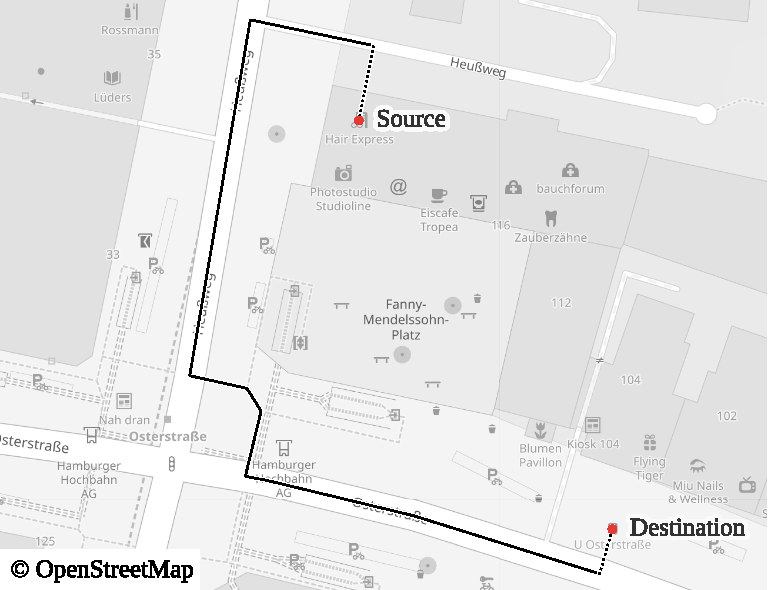
\includegraphics[width=0.65\textwidth]{images/qgis-routing-osterstrasse_routing.pdf}
				\end{figcenter}
				\caption{Graph-based routing result using the routing engine \href{https://www.osm.org/directions?engine=graphhopper\_foot\&route=53.57657,9.95210;53.57601,9.95268}{\emph{GraphHopper}}.}
			\end{figure}
		\end{frame}
	
		\begin{frame}[noframenumbering]{Example: Graph-based and geometric routing}
			\begin{figure}[t]
				\begin{figcenter}
					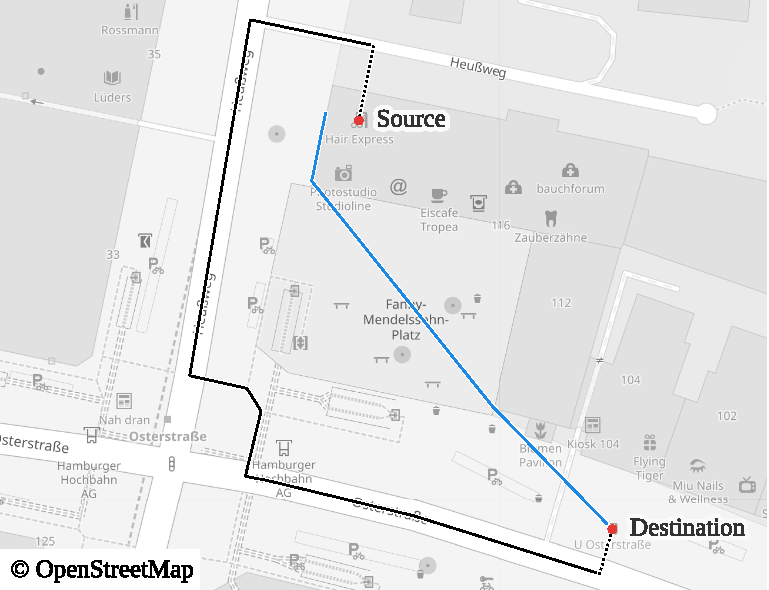
\includegraphics[width=0.65\textwidth]{images/qgis-routing-osterstrasse_routing-actual.pdf}
				\end{figcenter}
				\caption{Graph-based route (red) compared to the purely geometric route (blue).}
			\end{figure}
		\end{frame}
	
		\begin{frame}[noframenumbering]{Example: Graph-based and geometric routing}
			\begin{figure}[t]
				\begin{figcenter}
					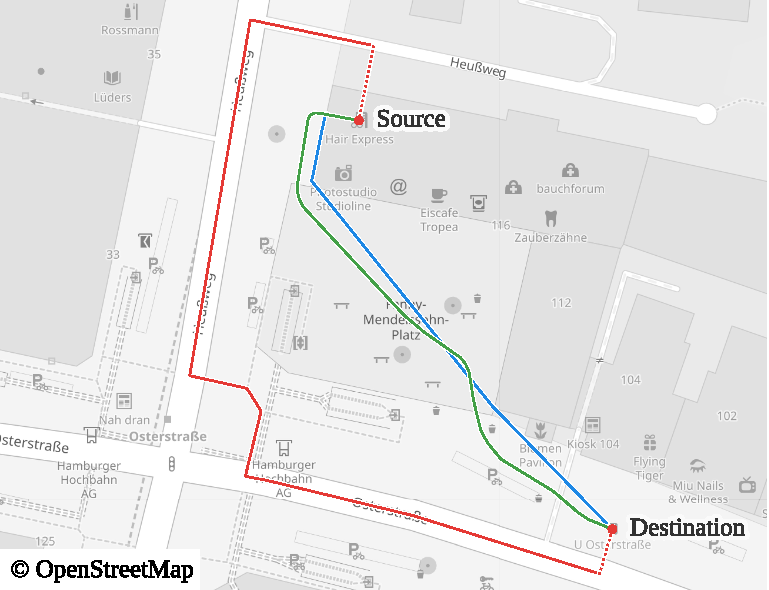
\includegraphics[width=0.65\textwidth]{images/qgis-routing-osterstrasse_routing-actual-expected.pdf}
				\end{figcenter}
				\caption{Graph-based (red), purely geometric (blue) and expected real-world route (green).}
			\end{figure}
		\end{frame}
		
		\begin{frame}{Value of graph data}
			Graph data is still valuable:\n
			\begin{itemize}
				\item detailed information
				\begin{itemize}
					\item e.g. surface conditions or access restrictions
				\end{itemize}
				\item definitely walkable
				\begin{itemize}
					\item bridges, tunnels, building passages
				\end{itemize}
			\end{itemize}
		\end{frame}
	
	\section{Design}
	
		\begin{frame}{Wanted routing algorithm}
			Should be able to\n
			\begin{itemize}
				\item use roads and ways
				\item traverse open spaces\ \textrightarrow\ reach arbitrary locations
				\item create realistic routes
			\end{itemize}
			\nn
			\pause
			Based on C\# / .NET, MARS (Multi-Agent Research and Simulation) and NTS (NetTopologySuite)
		\end{frame}
		
		\begin{frame}{Design decisions}
			Decisions of implemented algorithm:\n
			\begin{itemize}
				\item visibility graph generation
				\begin{itemize}
					\item custom algorithm
					\item algorithms from literature would have required additional adjustments
				\end{itemize}
				\item merge with existing road network
				\item connect source / destination with visibility edges
				\item usage of graph-based routing
			\end{itemize}
		\end{frame}
		
		\begin{frame}{Components}
			\begin{figure}[t]
				\begin{figcenter}
					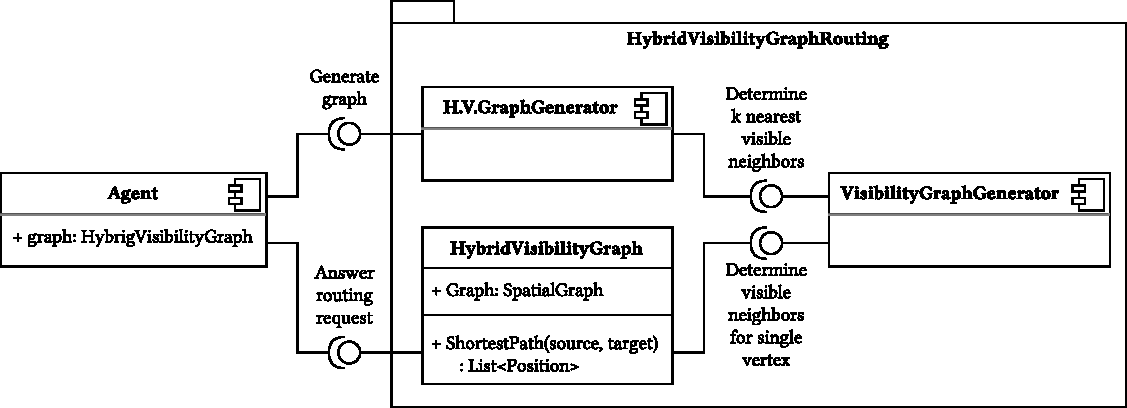
\includegraphics[width=0.95\textwidth]{images/components.pdf}
				\end{figcenter}
				\caption{Components of the implemented hybrid routing algorithm.}
			\end{figure}
		\end{frame}
	
	\section{Implementation}
	
		\begin{frame}{Considerations and terminology}
			Key considerations:\n
			\begin{itemize}
				\item implementation has to support
				\begin{itemize}
					\item collinear vertices
					\item arbitrary obstacle geometries (especially lines and polygons)
					\item intersecting obstacles
					\item arbitrary positions and non-unique coordinates
					\item[\textrightarrow] custom implementation instead of algorithm from the literature
				\end{itemize}
				\item generate and connect nodes suitable for routing
			\end{itemize}
			\nn
			\pause
			Terminology:\n
			\begin{description}[visibility neighbor]
				\item[obstacle neighbor] neighbor of $v$ on same or touching obstacle
				\item[visibility neighbor] visible neighbor of $v$ across open space
				\item[input vertex] vertex / coordinate in the input dataset
				\item[output vertex] generated vertex in the visibility graph
			\end{description}
		\end{frame}
		
		\begin{frame}{Hybrid visibility graph creation -- Overview}
			\begin{figure}[t]
				\begin{figcenter}
					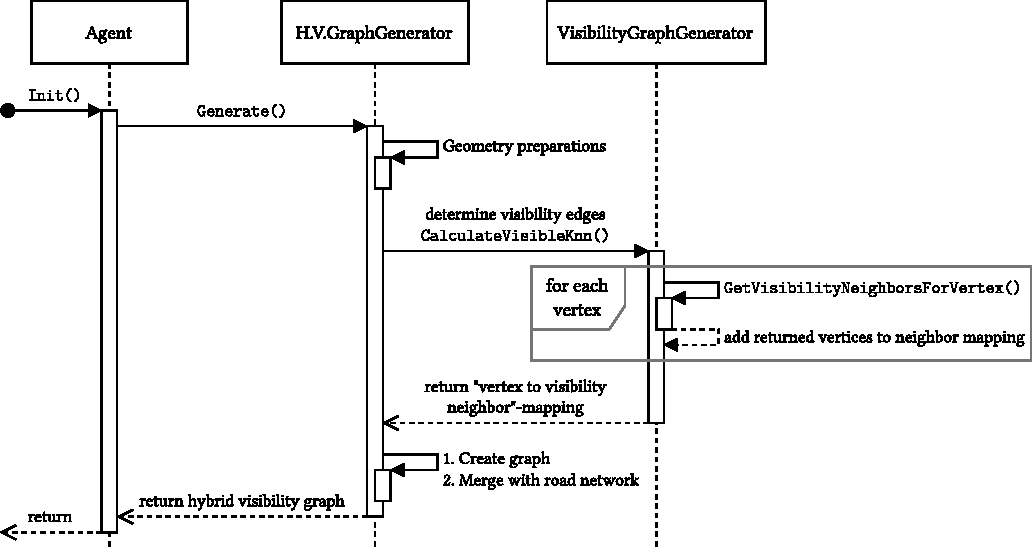
\includegraphics[width=0.98\textwidth]{images/components-sequence-generation-short.pdf}
				\end{figcenter}
				\caption{Separate steps of the graph generation.}
			\end{figure}
		\end{frame}
		
		\begin{frame}{Hybrid visibility graph creation -- Overview}
			\begin{enumerate}
				\item get and prepare obstacle geometries
				\begin{itemize}
					\item unwrap multi-geometries
					\item triangulate polygonal obstacles
					\begin{itemize}
						\item[\textrightarrow] performance optimization
					\end{itemize}
				\end{itemize}
				\item obtain data for visibility graph
				\begin{enumerate}
					\item for each vertex: determine its visibility neighbors
					\item group visibility neighbors based on obstacle neighbors
				\end{enumerate}
				\item generate routable visibility graph
				\item merge road edges
			\end{enumerate}
		\end{frame}
		
		\begin{frame}{Visibility graph creation}
			Naive approach:
			\begin{itemize}
				\item one vertex per input coordinate
				\item routing through line-based obstacles possible
			\end{itemize}
			\nn
			\pause
			My implementation:
			\begin{itemize}
				\item one vertex between adjacent obstacle neighbors
				\item multiple vertices at same location
				\item vertices are not connected
				\item routing through obstacle not possible
			\end{itemize}
		\end{frame}
	
		\begin{frame}{Visibility graph creation}
			\vspace{0.35cm}
			\begin{figure}
				\begin{figcenter}
					\scalebox{0.7}
					{
						\begin{tikzpicture}
	\tikzDot{(2,0)}{vo0};
	\tikzDot[label={[label distance=-1.25mm]above right:$v $}]{(2,1)}{vo1};
	\tikzDot{(2,2)}{vo2};
	
	\draw (vo0) -- (vo1);
	\draw (vo1) -- (vo2);
	
	\tikzDot[label=left:$n_a$,outer sep=0.5mm]{(0.5,1.3)}{n1};
	\tikzDot[label=right:$n_b$,outer sep=0.5mm]{(3.5,1)}{n2};
	
	\draw[dotted] (n1) -- (vo1);
	\draw[dotted] (vo1) -- (n2);
	
	\draw[dotted] (n1) -- (vo0);
	\draw[dotted] (n1) -- (vo2);
	\draw[dotted] (n2) -- (vo0);
	\draw[dotted] (n2) -- (vo2);
\end{tikzpicture}
					}
					\hspace{0.75cm}
					\scalebox{0.7}
					{
						\begin{tikzpicture}
	\def\r{0.85mm}
	\def\rMargin{1.1mm} % = r + 0.25mm
	\def\gap{0.1875mm}
	
	\tikzDot{(2,0)}{vo0};
	\node (vo1) at (2,1) {};
	\node[label={[label distance=-1.25mm]above left:$v_a$}] at (vo1) {};
	\node[label={[label distance=-1.25mm]above right:$v_b$}] at (vo1) {};
	\coordinate (vo11) at ($(vo1)+(180:\rMargin)$);
	\coordinate (vo12) at ($(vo1)+(0:\rMargin)$);
	\tikzDot{(2,2)}{vo2};
	
	\filldraw (vo1)++(-\gap,0)++(90:\r) arc (90:270:\r);
	\filldraw (vo1)++( \gap,0)++(90:\r) arc (90:-90:\r);
	
	\draw ($(vo1)+(270:\r)+(-0.275mm,0)$) -- ($(vo0)+(-0.275mm,2mm)$) -- (vo0.north);
	\draw ($(vo1)+(270:\r)+( 0.275mm,0)$) -- ($(vo0)+( 0.275mm,2mm)$) -- (vo0.north);
	
	\draw ($(vo1)+(90:\r)+(-0.275mm,0)$) -- ($(vo2)+(-0.275mm,-2mm)$) -- (vo2.south);
	\draw ($(vo1)+(90:\r)+( 0.275mm,0)$) -- ($(vo2)+( 0.275mm,-2mm)$) -- (vo2.south);
	
	\tikzDot[label=left:$n_a$,outer sep=0.5mm]{(0.5,1.3)}{n1};
	\tikzDot[label=right:$n_b$,outer sep=0.5mm]{(3.5,1)}{n2};
	
	\draw[dotted] (n1) -- (vo11);
	\draw[dotted] (vo12) -- (n2);
	
	\draw[dotted] (n1) -- (vo0);
	\draw[dotted] (n1) -- (vo2);
	\draw[dotted] (n2) -- (vo0);
	\draw[dotted] (n2) -- (vo2);
\end{tikzpicture}
					}
				\end{figcenter}
				\caption{Naive (left) and the implemented (right) vertex creation and connection.}
			\end{figure}
			\vspace{-0.3cm}
			\pause
			\begin{figure}
				\begin{figcenter}
					\scalebox{0.7}
					{
						\begin{tikzpicture}
	\def\d{0.03}
	
	\tikzDot[label=below:$v$]{(0,0)}{v}
	
	\tikzDot[label=left:$n_1$]{(-2.25,0)}{n1}
	\tikzDot[label=above:$n_2$]{(0,2)}{n2}
	\tikzDot[label=right:$n_3$]{(2.25,0)}{n3}
	
	\draw[lightgray] (v) -- (n1);
	\draw[lightgray] (v) -- (n3);
	\draw[lightgray] (v) -- (n2);
	
	% Visibility edges to n1
	\tikzDot[DodgerBlue3]{(-1.1,-0.25)}{vn1}
	\tikzDot[DodgerBlue3]{(-1.6,-0.9)}{vn2}
	\tikzDot[DodgerBlue3]{(1.6,-0.5)}{vn3}
	\draw[DodgerBlue3,densely dashed,->] (v) -- (vn1);
	\draw[DodgerBlue3,densely dashed,->] (v) -- (vn2);
	\draw[DodgerBlue3,densely dashed,->] (v) -- (vn3);
	
	% Visibility edges to n3
	\tikzDot[Red2]{(0.7,1.4)}{vn4}
	\tikzDot[Red2]{(2,1)}{vn5}
	\draw[Red2,densely dotted,->] (v) -- (vn4);
	\draw[Red2,densely dotted,->] (v) -- (vn5);
	
	% Visibility edges to n2
	\tikzDot[Green4]{(-2,1.3)}{vn6}
	\draw[Green4,dashdotted,->] (v) -- (vn6);
\end{tikzpicture}
					}
				\end{figcenter}
				\caption{Sorting visibility neighbors into bins, based on the obstacle neighbors of $v$.}
			\end{figure}
		\end{frame}
		
		\begin{frame}{Merging the road network}
			\begin{enumerate}
				\item create vertices at intersection points
				\item connect new vertex
				\item remove old edges
			\end{enumerate}
			\n
			\begin{figure}
				\begin{figcenter}
					\scalebox{0.7}
					{
						\begin{tikzpicture}
	\tikzDot{(0,-0.75)}{v1n1}
	\tikzDot{(4,-0.6)}{v1n2}
	
	\tikzDot{(0,0.8)}{v2n1}
	\tikzDot{(4.2,0.6)}{v2n2}
	
	\tikzDot{(1.5,-1.65)}{rn1}
	\tikzDot{(1.8,1.65)}{rn2}
	
	\draw[<->,dashed] (v1n1) -- node[above right=0cm and 0.4cm] {$v$} (v1n2);
	\draw[<->,dashed] (v2n1) -- node[above right=0cm and 0.4cm] {$u$} (v2n2);
	
	\draw[<->] (rn1) -- node[left] {$r$} (rn2);
\end{tikzpicture}
					}
					\hspace{0.75cm}
					\scalebox{0.7}
					{
						\begin{tikzpicture}
	\tikzDot{(0,-0.75)}{v1n1}
	\tikzDot{(4,-0.6)}{v1n2}
	
	\tikzDot{(0,0.8)}{v2n1}
	\tikzDot{(4.2,0.6)}{v2n2}
	
	\tikzDot{(1.5,-1.65)}{rn1}
	\tikzDot{(1.8,1.65)}{rn2}
	
	\tikzDot{(intersection of v1n1--v1n2 and rn1--rn2)}{i1}
	\tikzDot{(intersection of v2n1--v2n2 and rn1--rn2)}{i2}
	
	\draw[<->,dashed] (v1n1) -- node[above] {$v_1$} (i1);
	\draw[<->,dashed] (i1)   -- node[above] {$v_2$} (v1n2);
	\draw[<->,dashed] (v2n1) -- node[above] {$u_1$} (i2);
	\draw[<->,dashed] (i2)   -- node[above] {$u_2$} (v2n2);
	
	\draw[<->] (rn1) -- node[right] {$r_1$} (i1);
	\draw[<->] (i1)  -- node[right] {$r_2$} (i2);
	\draw[<->] (i2)  -- node[right] {$r_3$} (rn2);
\end{tikzpicture}
					}
				\end{figcenter}
				\caption{Merge of road network and visibility edges.}
			\end{figure}
		\end{frame}
		
		\begin{frame}{Answering routing queries}
			\begin{figure}[t]
				\begin{figcenter}
					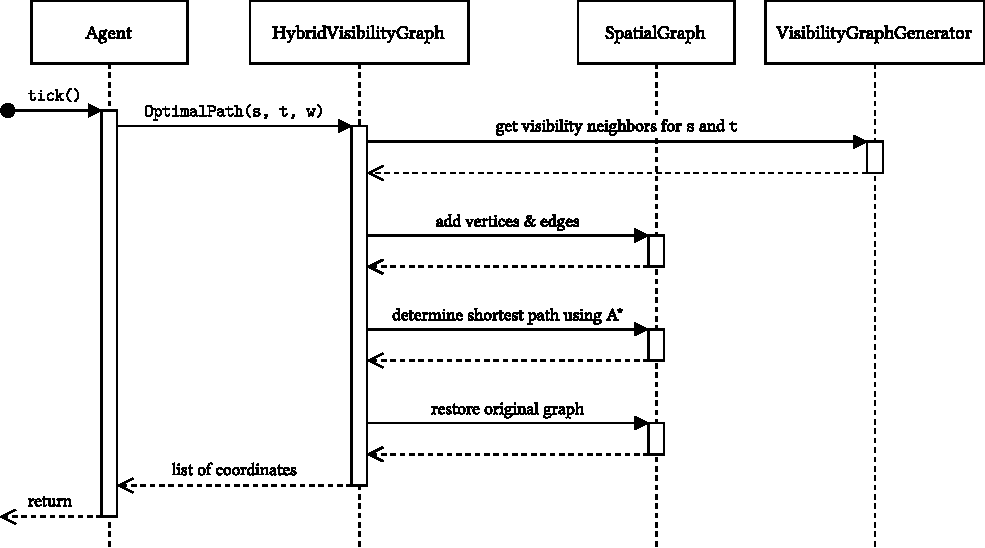
\includegraphics[width=0.95\textwidth]{images/components-sequence-routing-short.pdf}
				\end{figcenter}
				\caption{Separate steps of answering a routing request.}
			\end{figure}
		\end{frame}
		
		\begin{frame}{Performance optimizations -- Shadow areas}
			Exclude vertices in \enquote{shadow} of obstacles:\n
			\begin{itemize}
				\item consider vertex $v$ and think of it as light bulb
				\item obstacles cast shadow outwards, hiding vertices
			\end{itemize}
			\begin{figure}[b]
				\begin{figcenter}
					\scalebox{0.7}
					{
						\begin{tikzpicture}
	\def\angle{20}
	\def\boundingVertexDistance{3}
	
	\tikzDot[label=$v$]{(0,1.5)}{v}
	\coordinate (shadow-arc-top)				at ($(v) +( \angle:\boundingVertexDistance)$);
	\coordinate (shadow-arc-bottom)				at ($(v) +(-\angle:\boundingVertexDistance)$);
	\coordinate (shadow-arc-top-end)			at ($(v) +( \angle:5.75)$);
	\coordinate (shadow-arc-bottom-end)			at ($(v) +(-\angle:5.75)$);
	\coordinate (shadow-arc-top-faded-end)		at ($(v) +( \angle:6.5)$);
	\coordinate (shadow-arc-bottom-faded-end)	at ($(v) +(-\angle:6.5)$);
	
	% Gray area
	\filldraw[lightgray] 
	(shadow-arc-bottom) arc [start angle=-\angle, delta angle=2*\angle, radius=\boundingVertexDistance] --
	(shadow-arc-top-end) --
	(shadow-arc-bottom-end) --
	cycle;
	\draw[gray]
	(shadow-arc-bottom-end) --
	(shadow-arc-bottom) arc [start angle=-\angle, delta angle=2*\angle, radius=\boundingVertexDistance] --
	(shadow-arc-top-end);
	
	\draw[dotted] (v) -- (shadow-arc-top);
	\draw[dotted] (v) -- (shadow-arc-bottom);
	
	% Faded gray area
	\filldraw[draw=none,lightgray,path fading=east]
	(shadow-arc-top-faded-end) --
	(shadow-arc-top-end) --
	(shadow-arc-bottom-end) --
	(shadow-arc-bottom-faded-end) --
	cycle;
	\draw[gray,path fading=east] (shadow-arc-top-end) -- (shadow-arc-top-faded-end);
	\draw[gray,path fading=east] (shadow-arc-bottom-end) -- (shadow-arc-bottom-faded-end);
	
	% Obstacle
	\tikzDot[Red2]{(shadow-arc-top)}{o0}
	\tikzDot{(3.8,2)}{o1}
	\tikzDot[Red2]{($(v) +(-\angle:1.2)$)}{o2}
	\node[above right = 0.5 and 1.15 of o2] {$o$};
	
	% v' and v''
	\tikzDot[label=right:$v'$]{(2.1,1.1)}{v'}
	\tikzDot[label=right:$v''$]{(3.4,1.3)}{v''}
	
	\node[darkgray] at (4.7,1.5) {\huge$S$};
	
	\draw (o0) -- (o1) -- (o2) -- (o0);
\end{tikzpicture}

					}
				\end{figcenter}
				\caption{Shadow area $S$ cast by obstacle $o$.}
			\end{figure}
		\end{frame}
		
		\begin{frame}{Performance optimizations}
			Additional optimizations:
			\begin{itemize}
				\item usage of spatial indices
				\item custom intersection checks
				\item limiting number of visibility neighbors (kNN search)
				\item considering only vertices on convex hulls
				\item vertex filtering by irrelevant angular ranges
			\end{itemize}
		\end{frame}
	
	\section{Evaluation}
	
		\begin{frame}{Impact of optimizations}
			\begin{table}
				\begin{tabularx}{0.8\textwidth}{p{4.25cm}RR}
\toprule
\textbf{Enabled optimization}	& \textbf{Time}	& \textbf{Speedup}	\\
\midrule
Shadow areas					&  22.2 s		& 35.56				\\
kNN filtering					& 751.7 s		&  1.05				\\
Vertices on convex hull			& 287.9 s		&  2.74				\\
Valid angle areas				& 322.5 s		&  2.44				\\
Custom collision detection		& 769.3 s		&  1.02				\\
\midrule
No active optimization			& 788.5 s		&  1.00				\\
All optimizations active		&  11.1 s		& 71.13				\\
\bottomrule
				\end{tabularx}
				\caption{Impact of optimizations on the graph generation using the 0.5 km\textsuperscript{2} \enquote{OSM city} dataset.}
				\label{table:optimization-impact}
			\end{table}
		\end{frame}
		
		\begin{frame}{Real-world datasets}
			\begin{figure}
				\begin{figcenter}
					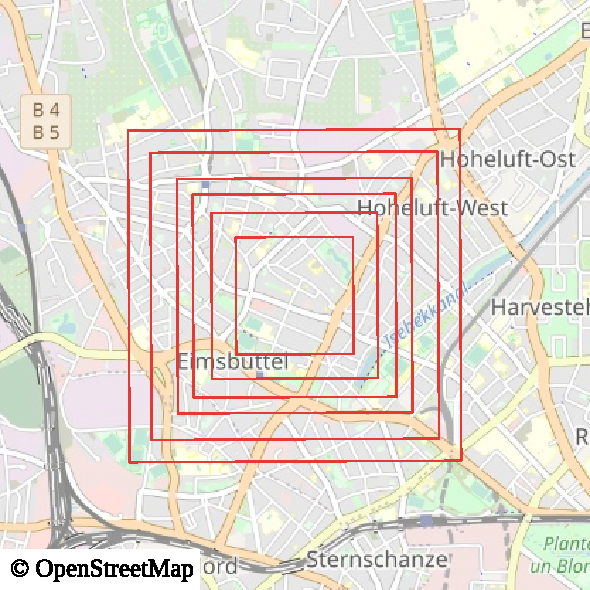
\includegraphics[width=0.45\textwidth]{images/qgis-overview-city.pdf}
					\hspace{0.5cm}
					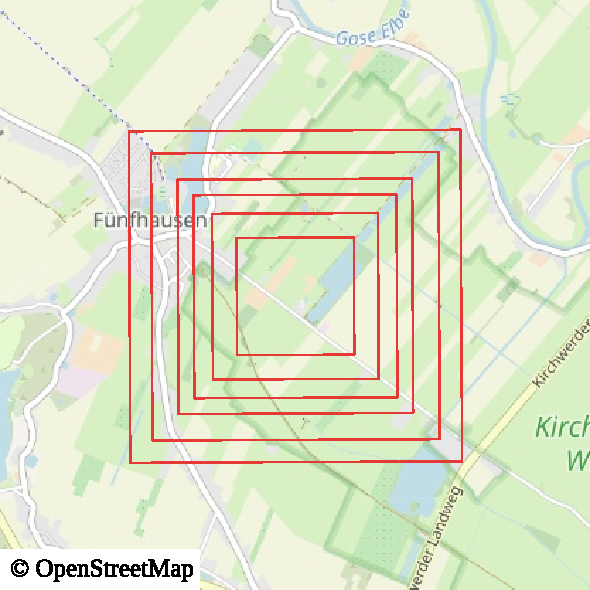
\includegraphics[width=0.45\textwidth]{images/qgis-overview-rural.pdf}
				\end{figcenter}
				\caption{Real-world datasets from the OpenStreetMap database used in the evaluation.}
			\end{figure}
		\end{frame}
		
		\begin{frame}{Graph generation task performance}
			\begin{figure}
				\begin{figcenter}
					\hspace*{-0.35cm}
					\scalebox{0.7}
					{
						%% Creator: Matplotlib, PGF backend
%%
%% To include the figure in your LaTeX document, write
%%   \input{<filename>.pgf}
%%
%% Make sure the required packages are loaded in your preamble
%%   \usepackage{pgf}
%%
%% Also ensure that all the required font packages are loaded; for instance,
%% the lmodern package is sometimes necessary when using math font.
%%   \usepackage{lmodern}
%%
%% Figures using additional raster images can only be included by \input if
%% they are in the same directory as the main LaTeX file. For loading figures
%% from other directories you can use the `import` package
%%   \usepackage{import}
%%
%% and then include the figures with
%%   \import{<path to file>}{<filename>.pgf}
%%
%% Matplotlib used the following preamble
%%   
%%   \usepackage{fontspec}
%%   \setmainfont{DejaVuSerif.ttf}[Path=\detokenize{/home/hauke/.local/lib/python3.11/site-packages/matplotlib/mpl-data/fonts/ttf/}]
%%   \setsansfont{DroidSans.ttf}[Path=\detokenize{/usr/share/fonts/droid/}]
%%   \setmonofont{DejaVuSansMono.ttf}[Path=\detokenize{/home/hauke/.local/lib/python3.11/site-packages/matplotlib/mpl-data/fonts/ttf/}]
%%   \makeatletter\@ifpackageloaded{underscore}{}{\usepackage[strings]{underscore}}\makeatother
%%
\begingroup%
\makeatletter%
\begin{pgfpicture}%
\pgfpathrectangle{\pgfpointorigin}{\pgfqpoint{6.101690in}{1.716449in}}%
\pgfusepath{use as bounding box, clip}%
\begin{pgfscope}%
\pgfsetbuttcap%
\pgfsetmiterjoin%
\definecolor{currentfill}{rgb}{1.000000,1.000000,1.000000}%
\pgfsetfillcolor{currentfill}%
\pgfsetlinewidth{0.000000pt}%
\definecolor{currentstroke}{rgb}{1.000000,1.000000,1.000000}%
\pgfsetstrokecolor{currentstroke}%
\pgfsetdash{}{0pt}%
\pgfpathmoveto{\pgfqpoint{0.000000in}{0.000000in}}%
\pgfpathlineto{\pgfqpoint{6.101690in}{0.000000in}}%
\pgfpathlineto{\pgfqpoint{6.101690in}{1.716449in}}%
\pgfpathlineto{\pgfqpoint{0.000000in}{1.716449in}}%
\pgfpathlineto{\pgfqpoint{0.000000in}{0.000000in}}%
\pgfpathclose%
\pgfusepath{fill}%
\end{pgfscope}%
\begin{pgfscope}%
\pgfsetbuttcap%
\pgfsetmiterjoin%
\definecolor{currentfill}{rgb}{1.000000,1.000000,1.000000}%
\pgfsetfillcolor{currentfill}%
\pgfsetlinewidth{0.000000pt}%
\definecolor{currentstroke}{rgb}{0.000000,0.000000,0.000000}%
\pgfsetstrokecolor{currentstroke}%
\pgfsetstrokeopacity{0.000000}%
\pgfsetdash{}{0pt}%
\pgfpathmoveto{\pgfqpoint{0.592976in}{0.400938in}}%
\pgfpathlineto{\pgfqpoint{4.765159in}{0.400938in}}%
\pgfpathlineto{\pgfqpoint{4.765159in}{1.716449in}}%
\pgfpathlineto{\pgfqpoint{0.592976in}{1.716449in}}%
\pgfpathlineto{\pgfqpoint{0.592976in}{0.400938in}}%
\pgfpathclose%
\pgfusepath{fill}%
\end{pgfscope}%
\begin{pgfscope}%
\definecolor{textcolor}{rgb}{0.150000,0.150000,0.150000}%
\pgfsetstrokecolor{textcolor}%
\pgfsetfillcolor{textcolor}%
\pgftext[x=0.940658in,y=0.268994in,,top]{\color{textcolor}\sffamily\fontsize{9.000000}{10.800000}\selectfont Total time}%
\end{pgfscope}%
\begin{pgfscope}%
\definecolor{textcolor}{rgb}{0.150000,0.150000,0.150000}%
\pgfsetstrokecolor{textcolor}%
\pgfsetfillcolor{textcolor}%
\pgftext[x=1.636022in,y=0.268994in,,top]{\color{textcolor}\sffamily\fontsize{9.000000}{10.800000}\selectfont kNN search}%
\end{pgfscope}%
\begin{pgfscope}%
\definecolor{textcolor}{rgb}{0.150000,0.150000,0.150000}%
\pgfsetstrokecolor{textcolor}%
\pgfsetfillcolor{textcolor}%
\pgftext[x=2.147517in, y=0.174023in, left, base]{\color{textcolor}\sffamily\fontsize{9.000000}{10.800000}\selectfont Create}%
\end{pgfscope}%
\begin{pgfscope}%
\definecolor{textcolor}{rgb}{0.150000,0.150000,0.150000}%
\pgfsetstrokecolor{textcolor}%
\pgfsetfillcolor{textcolor}%
\pgftext[x=2.168086in, y=0.030029in, left, base]{\color{textcolor}\sffamily\fontsize{9.000000}{10.800000}\selectfont graph}%
\end{pgfscope}%
\begin{pgfscope}%
\definecolor{textcolor}{rgb}{0.150000,0.150000,0.150000}%
\pgfsetstrokecolor{textcolor}%
\pgfsetfillcolor{textcolor}%
\pgftext[x=2.929002in, y=0.174023in, left, base]{\color{textcolor}\sffamily\fontsize{9.000000}{10.800000}\selectfont Get}%
\end{pgfscope}%
\begin{pgfscope}%
\definecolor{textcolor}{rgb}{0.150000,0.150000,0.150000}%
\pgfsetstrokecolor{textcolor}%
\pgfsetfillcolor{textcolor}%
\pgftext[x=2.764756in, y=0.030029in, left, base]{\color{textcolor}\sffamily\fontsize{9.000000}{10.800000}\selectfont obstacles}%
\end{pgfscope}%
\begin{pgfscope}%
\definecolor{textcolor}{rgb}{0.150000,0.150000,0.150000}%
\pgfsetstrokecolor{textcolor}%
\pgfsetfillcolor{textcolor}%
\pgftext[x=3.397101in, y=0.174023in, left, base]{\color{textcolor}\sffamily\fontsize{9.000000}{10.800000}\selectfont Merge road}%
\end{pgfscope}%
\begin{pgfscope}%
\definecolor{textcolor}{rgb}{0.150000,0.150000,0.150000}%
\pgfsetstrokecolor{textcolor}%
\pgfsetfillcolor{textcolor}%
\pgftext[x=3.558020in, y=0.030029in, left, base]{\color{textcolor}\sffamily\fontsize{9.000000}{10.800000}\selectfont edges}%
\end{pgfscope}%
\begin{pgfscope}%
\definecolor{textcolor}{rgb}{0.150000,0.150000,0.150000}%
\pgfsetstrokecolor{textcolor}%
\pgfsetfillcolor{textcolor}%
\pgftext[x=4.187039in, y=0.174023in, left, base]{\color{textcolor}\sffamily\fontsize{9.000000}{10.800000}\selectfont Add POI}%
\end{pgfscope}%
\begin{pgfscope}%
\definecolor{textcolor}{rgb}{0.150000,0.150000,0.150000}%
\pgfsetstrokecolor{textcolor}%
\pgfsetfillcolor{textcolor}%
\pgftext[x=4.143979in, y=0.030029in, left, base]{\color{textcolor}\sffamily\fontsize{9.000000}{10.800000}\selectfont attributes}%
\end{pgfscope}%
\begin{pgfscope}%
\pgfpathrectangle{\pgfqpoint{0.592976in}{0.400938in}}{\pgfqpoint{4.172183in}{1.315510in}}%
\pgfusepath{clip}%
\pgfsetroundcap%
\pgfsetroundjoin%
\pgfsetlinewidth{1.003750pt}%
\definecolor{currentstroke}{rgb}{0.800000,0.800000,0.800000}%
\pgfsetstrokecolor{currentstroke}%
\pgfsetdash{}{0pt}%
\pgfpathmoveto{\pgfqpoint{0.592976in}{0.628876in}}%
\pgfpathlineto{\pgfqpoint{4.765159in}{0.628876in}}%
\pgfusepath{stroke}%
\end{pgfscope}%
\begin{pgfscope}%
\definecolor{textcolor}{rgb}{0.150000,0.150000,0.150000}%
\pgfsetstrokecolor{textcolor}%
\pgfsetfillcolor{textcolor}%
\pgftext[x=0.194444in, y=0.581391in, left, base]{\color{textcolor}\sffamily\fontsize{9.000000}{10.800000}\selectfont \(\displaystyle {10^{-4}}\)}%
\end{pgfscope}%
\begin{pgfscope}%
\pgfpathrectangle{\pgfqpoint{0.592976in}{0.400938in}}{\pgfqpoint{4.172183in}{1.315510in}}%
\pgfusepath{clip}%
\pgfsetroundcap%
\pgfsetroundjoin%
\pgfsetlinewidth{1.003750pt}%
\definecolor{currentstroke}{rgb}{0.800000,0.800000,0.800000}%
\pgfsetstrokecolor{currentstroke}%
\pgfsetdash{}{0pt}%
\pgfpathmoveto{\pgfqpoint{0.592976in}{1.014126in}}%
\pgfpathlineto{\pgfqpoint{4.765159in}{1.014126in}}%
\pgfusepath{stroke}%
\end{pgfscope}%
\begin{pgfscope}%
\definecolor{textcolor}{rgb}{0.150000,0.150000,0.150000}%
\pgfsetstrokecolor{textcolor}%
\pgfsetfillcolor{textcolor}%
\pgftext[x=0.194444in, y=0.966641in, left, base]{\color{textcolor}\sffamily\fontsize{9.000000}{10.800000}\selectfont \(\displaystyle {10^{-2}}\)}%
\end{pgfscope}%
\begin{pgfscope}%
\pgfpathrectangle{\pgfqpoint{0.592976in}{0.400938in}}{\pgfqpoint{4.172183in}{1.315510in}}%
\pgfusepath{clip}%
\pgfsetroundcap%
\pgfsetroundjoin%
\pgfsetlinewidth{1.003750pt}%
\definecolor{currentstroke}{rgb}{0.800000,0.800000,0.800000}%
\pgfsetstrokecolor{currentstroke}%
\pgfsetdash{}{0pt}%
\pgfpathmoveto{\pgfqpoint{0.592976in}{1.399377in}}%
\pgfpathlineto{\pgfqpoint{4.765159in}{1.399377in}}%
\pgfusepath{stroke}%
\end{pgfscope}%
\begin{pgfscope}%
\definecolor{textcolor}{rgb}{0.150000,0.150000,0.150000}%
\pgfsetstrokecolor{textcolor}%
\pgfsetfillcolor{textcolor}%
\pgftext[x=0.274690in, y=1.351892in, left, base]{\color{textcolor}\sffamily\fontsize{9.000000}{10.800000}\selectfont \(\displaystyle {10^{0}}\)}%
\end{pgfscope}%
\begin{pgfscope}%
\definecolor{textcolor}{rgb}{0.150000,0.150000,0.150000}%
\pgfsetstrokecolor{textcolor}%
\pgfsetfillcolor{textcolor}%
\pgftext[x=0.125000in,y=1.058693in,,bottom,rotate=90.000000]{\color{textcolor}\sffamily\fontsize{9.000000}{10.800000}\selectfont Time in s}%
\end{pgfscope}%
\begin{pgfscope}%
\pgfpathrectangle{\pgfqpoint{0.592976in}{0.400938in}}{\pgfqpoint{4.172183in}{1.315510in}}%
\pgfusepath{clip}%
\pgfsetbuttcap%
\pgfsetmiterjoin%
\definecolor{currentfill}{rgb}{0.349020,0.490196,0.749020}%
\pgfsetfillcolor{currentfill}%
\pgfsetlinewidth{1.003750pt}%
\definecolor{currentstroke}{rgb}{1.000000,1.000000,1.000000}%
\pgfsetstrokecolor{currentstroke}%
\pgfsetdash{}{0pt}%
\pgfpathmoveto{\pgfqpoint{0.662512in}{-191.225881in}}%
\pgfpathlineto{\pgfqpoint{0.847943in}{-191.225881in}}%
\pgfpathlineto{\pgfqpoint{0.847943in}{1.656653in}}%
\pgfpathlineto{\pgfqpoint{0.662512in}{1.656653in}}%
\pgfpathlineto{\pgfqpoint{0.662512in}{-191.225881in}}%
\pgfpathclose%
\pgfusepath{stroke,fill}%
\end{pgfscope}%
\begin{pgfscope}%
\pgfpathrectangle{\pgfqpoint{0.592976in}{0.400938in}}{\pgfqpoint{4.172183in}{1.315510in}}%
\pgfusepath{clip}%
\pgfsetbuttcap%
\pgfsetmiterjoin%
\definecolor{currentfill}{rgb}{0.349020,0.490196,0.749020}%
\pgfsetfillcolor{currentfill}%
\pgfsetlinewidth{1.003750pt}%
\definecolor{currentstroke}{rgb}{1.000000,1.000000,1.000000}%
\pgfsetstrokecolor{currentstroke}%
\pgfsetdash{}{0pt}%
\pgfpathmoveto{\pgfqpoint{1.357876in}{-191.225881in}}%
\pgfpathlineto{\pgfqpoint{1.543307in}{-191.225881in}}%
\pgfpathlineto{\pgfqpoint{1.543307in}{1.577437in}}%
\pgfpathlineto{\pgfqpoint{1.357876in}{1.577437in}}%
\pgfpathlineto{\pgfqpoint{1.357876in}{-191.225881in}}%
\pgfpathclose%
\pgfusepath{stroke,fill}%
\end{pgfscope}%
\begin{pgfscope}%
\pgfpathrectangle{\pgfqpoint{0.592976in}{0.400938in}}{\pgfqpoint{4.172183in}{1.315510in}}%
\pgfusepath{clip}%
\pgfsetbuttcap%
\pgfsetmiterjoin%
\definecolor{currentfill}{rgb}{0.349020,0.490196,0.749020}%
\pgfsetfillcolor{currentfill}%
\pgfsetlinewidth{1.003750pt}%
\definecolor{currentstroke}{rgb}{1.000000,1.000000,1.000000}%
\pgfsetstrokecolor{currentstroke}%
\pgfsetdash{}{0pt}%
\pgfpathmoveto{\pgfqpoint{2.053240in}{-191.225881in}}%
\pgfpathlineto{\pgfqpoint{2.238670in}{-191.225881in}}%
\pgfpathlineto{\pgfqpoint{2.238670in}{1.271553in}}%
\pgfpathlineto{\pgfqpoint{2.053240in}{1.271553in}}%
\pgfpathlineto{\pgfqpoint{2.053240in}{-191.225881in}}%
\pgfpathclose%
\pgfusepath{stroke,fill}%
\end{pgfscope}%
\begin{pgfscope}%
\pgfpathrectangle{\pgfqpoint{0.592976in}{0.400938in}}{\pgfqpoint{4.172183in}{1.315510in}}%
\pgfusepath{clip}%
\pgfsetbuttcap%
\pgfsetmiterjoin%
\definecolor{currentfill}{rgb}{0.349020,0.490196,0.749020}%
\pgfsetfillcolor{currentfill}%
\pgfsetlinewidth{1.003750pt}%
\definecolor{currentstroke}{rgb}{1.000000,1.000000,1.000000}%
\pgfsetstrokecolor{currentstroke}%
\pgfsetdash{}{0pt}%
\pgfpathmoveto{\pgfqpoint{2.748604in}{-191.225881in}}%
\pgfpathlineto{\pgfqpoint{2.934034in}{-191.225881in}}%
\pgfpathlineto{\pgfqpoint{2.934034in}{1.085627in}}%
\pgfpathlineto{\pgfqpoint{2.748604in}{1.085627in}}%
\pgfpathlineto{\pgfqpoint{2.748604in}{-191.225881in}}%
\pgfpathclose%
\pgfusepath{stroke,fill}%
\end{pgfscope}%
\begin{pgfscope}%
\pgfpathrectangle{\pgfqpoint{0.592976in}{0.400938in}}{\pgfqpoint{4.172183in}{1.315510in}}%
\pgfusepath{clip}%
\pgfsetbuttcap%
\pgfsetmiterjoin%
\definecolor{currentfill}{rgb}{0.349020,0.490196,0.749020}%
\pgfsetfillcolor{currentfill}%
\pgfsetlinewidth{1.003750pt}%
\definecolor{currentstroke}{rgb}{1.000000,1.000000,1.000000}%
\pgfsetstrokecolor{currentstroke}%
\pgfsetdash{}{0pt}%
\pgfpathmoveto{\pgfqpoint{3.443968in}{-191.225881in}}%
\pgfpathlineto{\pgfqpoint{3.629398in}{-191.225881in}}%
\pgfpathlineto{\pgfqpoint{3.629398in}{1.613652in}}%
\pgfpathlineto{\pgfqpoint{3.443968in}{1.613652in}}%
\pgfpathlineto{\pgfqpoint{3.443968in}{-191.225881in}}%
\pgfpathclose%
\pgfusepath{stroke,fill}%
\end{pgfscope}%
\begin{pgfscope}%
\pgfpathrectangle{\pgfqpoint{0.592976in}{0.400938in}}{\pgfqpoint{4.172183in}{1.315510in}}%
\pgfusepath{clip}%
\pgfsetbuttcap%
\pgfsetmiterjoin%
\definecolor{currentfill}{rgb}{0.349020,0.490196,0.749020}%
\pgfsetfillcolor{currentfill}%
\pgfsetlinewidth{1.003750pt}%
\definecolor{currentstroke}{rgb}{1.000000,1.000000,1.000000}%
\pgfsetstrokecolor{currentstroke}%
\pgfsetdash{}{0pt}%
\pgfpathmoveto{\pgfqpoint{4.139332in}{-191.225881in}}%
\pgfpathlineto{\pgfqpoint{4.324762in}{-191.225881in}}%
\pgfpathlineto{\pgfqpoint{4.324762in}{0.865980in}}%
\pgfpathlineto{\pgfqpoint{4.139332in}{0.865980in}}%
\pgfpathlineto{\pgfqpoint{4.139332in}{-191.225881in}}%
\pgfpathclose%
\pgfusepath{stroke,fill}%
\end{pgfscope}%
\begin{pgfscope}%
\pgfpathrectangle{\pgfqpoint{0.592976in}{0.400938in}}{\pgfqpoint{4.172183in}{1.315510in}}%
\pgfusepath{clip}%
\pgfsetbuttcap%
\pgfsetmiterjoin%
\definecolor{currentfill}{rgb}{0.852941,0.544118,0.370588}%
\pgfsetfillcolor{currentfill}%
\pgfsetlinewidth{1.003750pt}%
\definecolor{currentstroke}{rgb}{1.000000,1.000000,1.000000}%
\pgfsetstrokecolor{currentstroke}%
\pgfsetdash{}{0pt}%
\pgfpathmoveto{\pgfqpoint{0.847943in}{-191.225881in}}%
\pgfpathlineto{\pgfqpoint{1.033373in}{-191.225881in}}%
\pgfpathlineto{\pgfqpoint{1.033373in}{1.580440in}}%
\pgfpathlineto{\pgfqpoint{0.847943in}{1.580440in}}%
\pgfpathlineto{\pgfqpoint{0.847943in}{-191.225881in}}%
\pgfpathclose%
\pgfusepath{stroke,fill}%
\end{pgfscope}%
\begin{pgfscope}%
\pgfpathrectangle{\pgfqpoint{0.592976in}{0.400938in}}{\pgfqpoint{4.172183in}{1.315510in}}%
\pgfusepath{clip}%
\pgfsetbuttcap%
\pgfsetmiterjoin%
\definecolor{currentfill}{rgb}{0.852941,0.544118,0.370588}%
\pgfsetfillcolor{currentfill}%
\pgfsetlinewidth{1.003750pt}%
\definecolor{currentstroke}{rgb}{1.000000,1.000000,1.000000}%
\pgfsetstrokecolor{currentstroke}%
\pgfsetdash{}{0pt}%
\pgfpathmoveto{\pgfqpoint{1.543307in}{-191.225881in}}%
\pgfpathlineto{\pgfqpoint{1.728737in}{-191.225881in}}%
\pgfpathlineto{\pgfqpoint{1.728737in}{1.577701in}}%
\pgfpathlineto{\pgfqpoint{1.543307in}{1.577701in}}%
\pgfpathlineto{\pgfqpoint{1.543307in}{-191.225881in}}%
\pgfpathclose%
\pgfusepath{stroke,fill}%
\end{pgfscope}%
\begin{pgfscope}%
\pgfpathrectangle{\pgfqpoint{0.592976in}{0.400938in}}{\pgfqpoint{4.172183in}{1.315510in}}%
\pgfusepath{clip}%
\pgfsetbuttcap%
\pgfsetmiterjoin%
\definecolor{currentfill}{rgb}{0.852941,0.544118,0.370588}%
\pgfsetfillcolor{currentfill}%
\pgfsetlinewidth{1.003750pt}%
\definecolor{currentstroke}{rgb}{1.000000,1.000000,1.000000}%
\pgfsetstrokecolor{currentstroke}%
\pgfsetdash{}{0pt}%
\pgfpathmoveto{\pgfqpoint{2.238670in}{-191.225881in}}%
\pgfpathlineto{\pgfqpoint{2.424101in}{-191.225881in}}%
\pgfpathlineto{\pgfqpoint{2.424101in}{1.276982in}}%
\pgfpathlineto{\pgfqpoint{2.238670in}{1.276982in}}%
\pgfpathlineto{\pgfqpoint{2.238670in}{-191.225881in}}%
\pgfpathclose%
\pgfusepath{stroke,fill}%
\end{pgfscope}%
\begin{pgfscope}%
\pgfpathrectangle{\pgfqpoint{0.592976in}{0.400938in}}{\pgfqpoint{4.172183in}{1.315510in}}%
\pgfusepath{clip}%
\pgfsetbuttcap%
\pgfsetmiterjoin%
\definecolor{currentfill}{rgb}{0.852941,0.544118,0.370588}%
\pgfsetfillcolor{currentfill}%
\pgfsetlinewidth{1.003750pt}%
\definecolor{currentstroke}{rgb}{1.000000,1.000000,1.000000}%
\pgfsetstrokecolor{currentstroke}%
\pgfsetdash{}{0pt}%
\pgfpathmoveto{\pgfqpoint{2.934034in}{-191.225881in}}%
\pgfpathlineto{\pgfqpoint{3.119465in}{-191.225881in}}%
\pgfpathlineto{\pgfqpoint{3.119465in}{1.088930in}}%
\pgfpathlineto{\pgfqpoint{2.934034in}{1.088930in}}%
\pgfpathlineto{\pgfqpoint{2.934034in}{-191.225881in}}%
\pgfpathclose%
\pgfusepath{stroke,fill}%
\end{pgfscope}%
\begin{pgfscope}%
\pgfpathrectangle{\pgfqpoint{0.592976in}{0.400938in}}{\pgfqpoint{4.172183in}{1.315510in}}%
\pgfusepath{clip}%
\pgfsetbuttcap%
\pgfsetmiterjoin%
\definecolor{currentfill}{rgb}{0.852941,0.544118,0.370588}%
\pgfsetfillcolor{currentfill}%
\pgfsetlinewidth{1.003750pt}%
\definecolor{currentstroke}{rgb}{1.000000,1.000000,1.000000}%
\pgfsetstrokecolor{currentstroke}%
\pgfsetdash{}{0pt}%
\pgfpathmoveto{\pgfqpoint{3.629398in}{-191.225881in}}%
\pgfpathlineto{\pgfqpoint{3.814829in}{-191.225881in}}%
\pgfpathlineto{\pgfqpoint{3.814829in}{0.853958in}}%
\pgfpathlineto{\pgfqpoint{3.629398in}{0.853958in}}%
\pgfpathlineto{\pgfqpoint{3.629398in}{-191.225881in}}%
\pgfpathclose%
\pgfusepath{stroke,fill}%
\end{pgfscope}%
\begin{pgfscope}%
\pgfpathrectangle{\pgfqpoint{0.592976in}{0.400938in}}{\pgfqpoint{4.172183in}{1.315510in}}%
\pgfusepath{clip}%
\pgfsetbuttcap%
\pgfsetmiterjoin%
\definecolor{currentfill}{rgb}{0.852941,0.544118,0.370588}%
\pgfsetfillcolor{currentfill}%
\pgfsetlinewidth{1.003750pt}%
\definecolor{currentstroke}{rgb}{1.000000,1.000000,1.000000}%
\pgfsetstrokecolor{currentstroke}%
\pgfsetdash{}{0pt}%
\pgfpathmoveto{\pgfqpoint{4.324762in}{-191.225881in}}%
\pgfpathlineto{\pgfqpoint{4.510193in}{-191.225881in}}%
\pgfpathlineto{\pgfqpoint{4.510193in}{0.852688in}}%
\pgfpathlineto{\pgfqpoint{4.324762in}{0.852688in}}%
\pgfpathlineto{\pgfqpoint{4.324762in}{-191.225881in}}%
\pgfpathclose%
\pgfusepath{stroke,fill}%
\end{pgfscope}%
\begin{pgfscope}%
\pgfpathrectangle{\pgfqpoint{0.592976in}{0.400938in}}{\pgfqpoint{4.172183in}{1.315510in}}%
\pgfusepath{clip}%
\pgfsetbuttcap%
\pgfsetmiterjoin%
\definecolor{currentfill}{rgb}{0.460784,0.749020,0.443137}%
\pgfsetfillcolor{currentfill}%
\pgfsetlinewidth{1.003750pt}%
\definecolor{currentstroke}{rgb}{1.000000,1.000000,1.000000}%
\pgfsetstrokecolor{currentstroke}%
\pgfsetdash{}{0pt}%
\pgfpathmoveto{\pgfqpoint{1.033373in}{-191.225881in}}%
\pgfpathlineto{\pgfqpoint{1.218803in}{-191.225881in}}%
\pgfpathlineto{\pgfqpoint{1.218803in}{1.129470in}}%
\pgfpathlineto{\pgfqpoint{1.033373in}{1.129470in}}%
\pgfpathlineto{\pgfqpoint{1.033373in}{-191.225881in}}%
\pgfpathclose%
\pgfusepath{stroke,fill}%
\end{pgfscope}%
\begin{pgfscope}%
\pgfpathrectangle{\pgfqpoint{0.592976in}{0.400938in}}{\pgfqpoint{4.172183in}{1.315510in}}%
\pgfusepath{clip}%
\pgfsetbuttcap%
\pgfsetmiterjoin%
\definecolor{currentfill}{rgb}{0.460784,0.749020,0.443137}%
\pgfsetfillcolor{currentfill}%
\pgfsetlinewidth{1.003750pt}%
\definecolor{currentstroke}{rgb}{1.000000,1.000000,1.000000}%
\pgfsetstrokecolor{currentstroke}%
\pgfsetdash{}{0pt}%
\pgfpathmoveto{\pgfqpoint{1.728737in}{-191.225881in}}%
\pgfpathlineto{\pgfqpoint{1.914167in}{-191.225881in}}%
\pgfpathlineto{\pgfqpoint{1.914167in}{0.460734in}}%
\pgfpathlineto{\pgfqpoint{1.728737in}{0.460734in}}%
\pgfpathlineto{\pgfqpoint{1.728737in}{-191.225881in}}%
\pgfpathclose%
\pgfusepath{stroke,fill}%
\end{pgfscope}%
\begin{pgfscope}%
\pgfpathrectangle{\pgfqpoint{0.592976in}{0.400938in}}{\pgfqpoint{4.172183in}{1.315510in}}%
\pgfusepath{clip}%
\pgfsetbuttcap%
\pgfsetmiterjoin%
\definecolor{currentfill}{rgb}{0.460784,0.749020,0.443137}%
\pgfsetfillcolor{currentfill}%
\pgfsetlinewidth{1.003750pt}%
\definecolor{currentstroke}{rgb}{1.000000,1.000000,1.000000}%
\pgfsetstrokecolor{currentstroke}%
\pgfsetdash{}{0pt}%
\pgfpathmoveto{\pgfqpoint{2.424101in}{-191.225881in}}%
\pgfpathlineto{\pgfqpoint{2.609531in}{-191.225881in}}%
\pgfpathlineto{\pgfqpoint{2.609531in}{0.460734in}}%
\pgfpathlineto{\pgfqpoint{2.424101in}{0.460734in}}%
\pgfpathlineto{\pgfqpoint{2.424101in}{-191.225881in}}%
\pgfpathclose%
\pgfusepath{stroke,fill}%
\end{pgfscope}%
\begin{pgfscope}%
\pgfpathrectangle{\pgfqpoint{0.592976in}{0.400938in}}{\pgfqpoint{4.172183in}{1.315510in}}%
\pgfusepath{clip}%
\pgfsetbuttcap%
\pgfsetmiterjoin%
\definecolor{currentfill}{rgb}{0.460784,0.749020,0.443137}%
\pgfsetfillcolor{currentfill}%
\pgfsetlinewidth{1.003750pt}%
\definecolor{currentstroke}{rgb}{1.000000,1.000000,1.000000}%
\pgfsetstrokecolor{currentstroke}%
\pgfsetdash{}{0pt}%
\pgfpathmoveto{\pgfqpoint{3.119465in}{-191.225881in}}%
\pgfpathlineto{\pgfqpoint{3.304895in}{-191.225881in}}%
\pgfpathlineto{\pgfqpoint{3.304895in}{0.795676in}}%
\pgfpathlineto{\pgfqpoint{3.119465in}{0.795676in}}%
\pgfpathlineto{\pgfqpoint{3.119465in}{-191.225881in}}%
\pgfpathclose%
\pgfusepath{stroke,fill}%
\end{pgfscope}%
\begin{pgfscope}%
\pgfpathrectangle{\pgfqpoint{0.592976in}{0.400938in}}{\pgfqpoint{4.172183in}{1.315510in}}%
\pgfusepath{clip}%
\pgfsetbuttcap%
\pgfsetmiterjoin%
\definecolor{currentfill}{rgb}{0.460784,0.749020,0.443137}%
\pgfsetfillcolor{currentfill}%
\pgfsetlinewidth{1.003750pt}%
\definecolor{currentstroke}{rgb}{1.000000,1.000000,1.000000}%
\pgfsetstrokecolor{currentstroke}%
\pgfsetdash{}{0pt}%
\pgfpathmoveto{\pgfqpoint{3.814829in}{-191.225881in}}%
\pgfpathlineto{\pgfqpoint{4.000259in}{-191.225881in}}%
\pgfpathlineto{\pgfqpoint{4.000259in}{1.120340in}}%
\pgfpathlineto{\pgfqpoint{3.814829in}{1.120340in}}%
\pgfpathlineto{\pgfqpoint{3.814829in}{-191.225881in}}%
\pgfpathclose%
\pgfusepath{stroke,fill}%
\end{pgfscope}%
\begin{pgfscope}%
\pgfpathrectangle{\pgfqpoint{0.592976in}{0.400938in}}{\pgfqpoint{4.172183in}{1.315510in}}%
\pgfusepath{clip}%
\pgfsetbuttcap%
\pgfsetmiterjoin%
\definecolor{currentfill}{rgb}{0.460784,0.749020,0.443137}%
\pgfsetfillcolor{currentfill}%
\pgfsetlinewidth{1.003750pt}%
\definecolor{currentstroke}{rgb}{1.000000,1.000000,1.000000}%
\pgfsetstrokecolor{currentstroke}%
\pgfsetdash{}{0pt}%
\pgfpathmoveto{\pgfqpoint{4.510193in}{-191.225881in}}%
\pgfpathlineto{\pgfqpoint{4.695623in}{-191.225881in}}%
\pgfpathlineto{\pgfqpoint{4.695623in}{0.746709in}}%
\pgfpathlineto{\pgfqpoint{4.510193in}{0.746709in}}%
\pgfpathlineto{\pgfqpoint{4.510193in}{-191.225881in}}%
\pgfpathclose%
\pgfusepath{stroke,fill}%
\end{pgfscope}%
\begin{pgfscope}%
\pgfsetrectcap%
\pgfsetmiterjoin%
\pgfsetlinewidth{1.254687pt}%
\definecolor{currentstroke}{rgb}{0.800000,0.800000,0.800000}%
\pgfsetstrokecolor{currentstroke}%
\pgfsetdash{}{0pt}%
\pgfpathmoveto{\pgfqpoint{0.592976in}{0.400938in}}%
\pgfpathlineto{\pgfqpoint{0.592976in}{1.716449in}}%
\pgfusepath{stroke}%
\end{pgfscope}%
\begin{pgfscope}%
\pgfsetrectcap%
\pgfsetmiterjoin%
\pgfsetlinewidth{1.254687pt}%
\definecolor{currentstroke}{rgb}{0.800000,0.800000,0.800000}%
\pgfsetstrokecolor{currentstroke}%
\pgfsetdash{}{0pt}%
\pgfpathmoveto{\pgfqpoint{4.765159in}{0.400938in}}%
\pgfpathlineto{\pgfqpoint{4.765159in}{1.716449in}}%
\pgfusepath{stroke}%
\end{pgfscope}%
\begin{pgfscope}%
\pgfsetrectcap%
\pgfsetmiterjoin%
\pgfsetlinewidth{1.254687pt}%
\definecolor{currentstroke}{rgb}{0.800000,0.800000,0.800000}%
\pgfsetstrokecolor{currentstroke}%
\pgfsetdash{}{0pt}%
\pgfpathmoveto{\pgfqpoint{0.592976in}{0.400938in}}%
\pgfpathlineto{\pgfqpoint{4.765159in}{0.400938in}}%
\pgfusepath{stroke}%
\end{pgfscope}%
\begin{pgfscope}%
\pgfsetrectcap%
\pgfsetmiterjoin%
\pgfsetlinewidth{1.254687pt}%
\definecolor{currentstroke}{rgb}{0.800000,0.800000,0.800000}%
\pgfsetstrokecolor{currentstroke}%
\pgfsetdash{}{0pt}%
\pgfpathmoveto{\pgfqpoint{0.592976in}{1.716449in}}%
\pgfpathlineto{\pgfqpoint{4.765159in}{1.716449in}}%
\pgfusepath{stroke}%
\end{pgfscope}%
\begin{pgfscope}%
\pgfsetbuttcap%
\pgfsetmiterjoin%
\definecolor{currentfill}{rgb}{1.000000,1.000000,1.000000}%
\pgfsetfillcolor{currentfill}%
\pgfsetfillopacity{0.800000}%
\pgfsetlinewidth{1.003750pt}%
\definecolor{currentstroke}{rgb}{0.800000,0.800000,0.800000}%
\pgfsetstrokecolor{currentstroke}%
\pgfsetstrokeopacity{0.800000}%
\pgfsetdash{}{0pt}%
\pgfpathmoveto{\pgfqpoint{4.956964in}{0.664944in}}%
\pgfpathlineto{\pgfqpoint{6.076690in}{0.664944in}}%
\pgfpathquadraticcurveto{\pgfqpoint{6.101690in}{0.664944in}}{\pgfqpoint{6.101690in}{0.689944in}}%
\pgfpathlineto{\pgfqpoint{6.101690in}{1.427443in}}%
\pgfpathquadraticcurveto{\pgfqpoint{6.101690in}{1.452443in}}{\pgfqpoint{6.076690in}{1.452443in}}%
\pgfpathlineto{\pgfqpoint{4.956964in}{1.452443in}}%
\pgfpathquadraticcurveto{\pgfqpoint{4.931964in}{1.452443in}}{\pgfqpoint{4.931964in}{1.427443in}}%
\pgfpathlineto{\pgfqpoint{4.931964in}{0.689944in}}%
\pgfpathquadraticcurveto{\pgfqpoint{4.931964in}{0.664944in}}{\pgfqpoint{4.956964in}{0.664944in}}%
\pgfpathlineto{\pgfqpoint{4.956964in}{0.664944in}}%
\pgfpathclose%
\pgfusepath{stroke,fill}%
\end{pgfscope}%
\begin{pgfscope}%
\definecolor{textcolor}{rgb}{0.150000,0.150000,0.150000}%
\pgfsetstrokecolor{textcolor}%
\pgfsetfillcolor{textcolor}%
\pgftext[x=5.303723in,y=1.307472in,left,base]{\color{textcolor}\sffamily\fontsize{9.000000}{10.800000}\selectfont Dataset}%
\end{pgfscope}%
\begin{pgfscope}%
\pgfsetbuttcap%
\pgfsetmiterjoin%
\definecolor{currentfill}{rgb}{0.349020,0.490196,0.749020}%
\pgfsetfillcolor{currentfill}%
\pgfsetlinewidth{1.003750pt}%
\definecolor{currentstroke}{rgb}{1.000000,1.000000,1.000000}%
\pgfsetstrokecolor{currentstroke}%
\pgfsetdash{}{0pt}%
\pgfpathmoveto{\pgfqpoint{4.981964in}{1.119973in}}%
\pgfpathlineto{\pgfqpoint{5.231964in}{1.119973in}}%
\pgfpathlineto{\pgfqpoint{5.231964in}{1.207473in}}%
\pgfpathlineto{\pgfqpoint{4.981964in}{1.207473in}}%
\pgfpathlineto{\pgfqpoint{4.981964in}{1.119973in}}%
\pgfpathclose%
\pgfusepath{stroke,fill}%
\end{pgfscope}%
\begin{pgfscope}%
\definecolor{textcolor}{rgb}{0.150000,0.150000,0.150000}%
\pgfsetstrokecolor{textcolor}%
\pgfsetfillcolor{textcolor}%
\pgftext[x=5.331964in,y=1.119973in,left,base]{\color{textcolor}\sffamily\fontsize{9.000000}{10.800000}\selectfont Normal}%
\end{pgfscope}%
\begin{pgfscope}%
\pgfsetbuttcap%
\pgfsetmiterjoin%
\definecolor{currentfill}{rgb}{0.852941,0.544118,0.370588}%
\pgfsetfillcolor{currentfill}%
\pgfsetlinewidth{1.003750pt}%
\definecolor{currentstroke}{rgb}{1.000000,1.000000,1.000000}%
\pgfsetstrokecolor{currentstroke}%
\pgfsetdash{}{0pt}%
\pgfpathmoveto{\pgfqpoint{4.981964in}{0.932473in}}%
\pgfpathlineto{\pgfqpoint{5.231964in}{0.932473in}}%
\pgfpathlineto{\pgfqpoint{5.231964in}{1.019973in}}%
\pgfpathlineto{\pgfqpoint{4.981964in}{1.019973in}}%
\pgfpathlineto{\pgfqpoint{4.981964in}{0.932473in}}%
\pgfpathclose%
\pgfusepath{stroke,fill}%
\end{pgfscope}%
\begin{pgfscope}%
\definecolor{textcolor}{rgb}{0.150000,0.150000,0.150000}%
\pgfsetstrokecolor{textcolor}%
\pgfsetfillcolor{textcolor}%
\pgftext[x=5.331964in,y=0.932473in,left,base]{\color{textcolor}\sffamily\fontsize{9.000000}{10.800000}\selectfont No roads}%
\end{pgfscope}%
\begin{pgfscope}%
\pgfsetbuttcap%
\pgfsetmiterjoin%
\definecolor{currentfill}{rgb}{0.460784,0.749020,0.443137}%
\pgfsetfillcolor{currentfill}%
\pgfsetlinewidth{1.003750pt}%
\definecolor{currentstroke}{rgb}{1.000000,1.000000,1.000000}%
\pgfsetstrokecolor{currentstroke}%
\pgfsetdash{}{0pt}%
\pgfpathmoveto{\pgfqpoint{4.981964in}{0.744973in}}%
\pgfpathlineto{\pgfqpoint{5.231964in}{0.744973in}}%
\pgfpathlineto{\pgfqpoint{5.231964in}{0.832473in}}%
\pgfpathlineto{\pgfqpoint{4.981964in}{0.832473in}}%
\pgfpathlineto{\pgfqpoint{4.981964in}{0.744973in}}%
\pgfpathclose%
\pgfusepath{stroke,fill}%
\end{pgfscope}%
\begin{pgfscope}%
\definecolor{textcolor}{rgb}{0.150000,0.150000,0.150000}%
\pgfsetstrokecolor{textcolor}%
\pgfsetfillcolor{textcolor}%
\pgftext[x=5.331964in,y=0.744973in,left,base]{\color{textcolor}\sffamily\fontsize{9.000000}{10.800000}\selectfont No obstacles}%
\end{pgfscope}%
\end{pgfpicture}%
\makeatother%
\endgroup%

					}
				\end{figcenter}
				\caption{Time of graph generation tasks on different variants of the 4 km\textsuperscript{2} \enquote{OSM city} dataset.}
			\end{figure}
		\end{frame}
		
		\begin{frame}{Graph generation task performance}
			\begin{figure}
				\begin{figcenter}
					\hspace*{-0.35cm}
					\scalebox{0.7}
					{
						\begingroup%
\makeatletter%
\begin{pgfpicture}%
\pgfpathrectangle{\pgfpointorigin}{\pgfqpoint{6.057453in}{2.407638in}}%
\pgfusepath{use as bounding box}%
\begin{pgfscope}%
\pgfsetbuttcap%
\pgfsetmiterjoin%
\definecolor{currentfill}{rgb}{1.000000,1.000000,1.000000}%
\pgfsetfillcolor{currentfill}%
\pgfsetlinewidth{0.000000pt}%
\definecolor{currentstroke}{rgb}{1.000000,1.000000,1.000000}%
\pgfsetstrokecolor{currentstroke}%
\pgfsetdash{}{0pt}%
\pgfpathmoveto{\pgfqpoint{0.000000in}{0.000000in}}%
\pgfpathlineto{\pgfqpoint{6.057453in}{0.000000in}}%
\pgfpathlineto{\pgfqpoint{6.057453in}{2.407638in}}%
\pgfpathlineto{\pgfqpoint{0.000000in}{2.407638in}}%
\pgfpathlineto{\pgfqpoint{0.000000in}{0.000000in}}%
\pgfpathclose%
\pgfusepath{fill}%
\end{pgfscope}%
\begin{pgfscope}%
\pgfsetbuttcap%
\pgfsetmiterjoin%
\definecolor{currentfill}{rgb}{1.000000,1.000000,1.000000}%
\pgfsetfillcolor{currentfill}%
\pgfsetlinewidth{0.000000pt}%
\definecolor{currentstroke}{rgb}{0.000000,0.000000,0.000000}%
\pgfsetstrokecolor{currentstroke}%
\pgfsetstrokeopacity{0.000000}%
\pgfsetdash{}{0pt}%
\pgfpathmoveto{\pgfqpoint{0.592976in}{0.451389in}}%
\pgfpathlineto{\pgfqpoint{4.648997in}{0.451389in}}%
\pgfpathlineto{\pgfqpoint{4.648997in}{2.407638in}}%
\pgfpathlineto{\pgfqpoint{0.592976in}{2.407638in}}%
\pgfpathlineto{\pgfqpoint{0.592976in}{0.451389in}}%
\pgfpathclose%
\pgfusepath{fill}%
\end{pgfscope}%
\begin{pgfscope}%
\pgfpathrectangle{\pgfqpoint{0.592976in}{0.451389in}}{\pgfqpoint{4.056021in}{1.956249in}}%
\pgfusepath{clip}%
\pgfsetroundcap%
\pgfsetroundjoin%
\pgfsetlinewidth{1.003750pt}%
\definecolor{currentstroke}{rgb}{0.800000,0.800000,0.800000}%
\pgfsetstrokecolor{currentstroke}%
\pgfsetdash{}{0pt}%
\pgfpathmoveto{\pgfqpoint{1.059707in}{0.451389in}}%
\pgfpathlineto{\pgfqpoint{1.059707in}{2.407638in}}%
\pgfusepath{stroke}%
\end{pgfscope}%
\begin{pgfscope}%
\definecolor{textcolor}{rgb}{0.150000,0.150000,0.150000}%
\pgfsetstrokecolor{textcolor}%
\pgfsetfillcolor{textcolor}%
\pgftext[x=1.059707in,y=0.319444in,,top]{\color{textcolor}\sffamily\fontsize{9.000000}{10.800000}\selectfont 10000}%
\end{pgfscope}%
\begin{pgfscope}%
\pgfpathrectangle{\pgfqpoint{0.592976in}{0.451389in}}{\pgfqpoint{4.056021in}{1.956249in}}%
\pgfusepath{clip}%
\pgfsetroundcap%
\pgfsetroundjoin%
\pgfsetlinewidth{1.003750pt}%
\definecolor{currentstroke}{rgb}{0.800000,0.800000,0.800000}%
\pgfsetstrokecolor{currentstroke}%
\pgfsetdash{}{0pt}%
\pgfpathmoveto{\pgfqpoint{1.545875in}{0.451389in}}%
\pgfpathlineto{\pgfqpoint{1.545875in}{2.407638in}}%
\pgfusepath{stroke}%
\end{pgfscope}%
\begin{pgfscope}%
\definecolor{textcolor}{rgb}{0.150000,0.150000,0.150000}%
\pgfsetstrokecolor{textcolor}%
\pgfsetfillcolor{textcolor}%
\pgftext[x=1.545875in,y=0.319444in,,top]{\color{textcolor}\sffamily\fontsize{9.000000}{10.800000}\selectfont 15000}%
\end{pgfscope}%
\begin{pgfscope}%
\pgfpathrectangle{\pgfqpoint{0.592976in}{0.451389in}}{\pgfqpoint{4.056021in}{1.956249in}}%
\pgfusepath{clip}%
\pgfsetroundcap%
\pgfsetroundjoin%
\pgfsetlinewidth{1.003750pt}%
\definecolor{currentstroke}{rgb}{0.800000,0.800000,0.800000}%
\pgfsetstrokecolor{currentstroke}%
\pgfsetdash{}{0pt}%
\pgfpathmoveto{\pgfqpoint{2.032043in}{0.451389in}}%
\pgfpathlineto{\pgfqpoint{2.032043in}{2.407638in}}%
\pgfusepath{stroke}%
\end{pgfscope}%
\begin{pgfscope}%
\definecolor{textcolor}{rgb}{0.150000,0.150000,0.150000}%
\pgfsetstrokecolor{textcolor}%
\pgfsetfillcolor{textcolor}%
\pgftext[x=2.032043in,y=0.319444in,,top]{\color{textcolor}\sffamily\fontsize{9.000000}{10.800000}\selectfont 20000}%
\end{pgfscope}%
\begin{pgfscope}%
\pgfpathrectangle{\pgfqpoint{0.592976in}{0.451389in}}{\pgfqpoint{4.056021in}{1.956249in}}%
\pgfusepath{clip}%
\pgfsetroundcap%
\pgfsetroundjoin%
\pgfsetlinewidth{1.003750pt}%
\definecolor{currentstroke}{rgb}{0.800000,0.800000,0.800000}%
\pgfsetstrokecolor{currentstroke}%
\pgfsetdash{}{0pt}%
\pgfpathmoveto{\pgfqpoint{2.518211in}{0.451389in}}%
\pgfpathlineto{\pgfqpoint{2.518211in}{2.407638in}}%
\pgfusepath{stroke}%
\end{pgfscope}%
\begin{pgfscope}%
\definecolor{textcolor}{rgb}{0.150000,0.150000,0.150000}%
\pgfsetstrokecolor{textcolor}%
\pgfsetfillcolor{textcolor}%
\pgftext[x=2.518211in,y=0.319444in,,top]{\color{textcolor}\sffamily\fontsize{9.000000}{10.800000}\selectfont 25000}%
\end{pgfscope}%
\begin{pgfscope}%
\pgfpathrectangle{\pgfqpoint{0.592976in}{0.451389in}}{\pgfqpoint{4.056021in}{1.956249in}}%
\pgfusepath{clip}%
\pgfsetroundcap%
\pgfsetroundjoin%
\pgfsetlinewidth{1.003750pt}%
\definecolor{currentstroke}{rgb}{0.800000,0.800000,0.800000}%
\pgfsetstrokecolor{currentstroke}%
\pgfsetdash{}{0pt}%
\pgfpathmoveto{\pgfqpoint{3.004379in}{0.451389in}}%
\pgfpathlineto{\pgfqpoint{3.004379in}{2.407638in}}%
\pgfusepath{stroke}%
\end{pgfscope}%
\begin{pgfscope}%
\definecolor{textcolor}{rgb}{0.150000,0.150000,0.150000}%
\pgfsetstrokecolor{textcolor}%
\pgfsetfillcolor{textcolor}%
\pgftext[x=3.004379in,y=0.319444in,,top]{\color{textcolor}\sffamily\fontsize{9.000000}{10.800000}\selectfont 30000}%
\end{pgfscope}%
\begin{pgfscope}%
\pgfpathrectangle{\pgfqpoint{0.592976in}{0.451389in}}{\pgfqpoint{4.056021in}{1.956249in}}%
\pgfusepath{clip}%
\pgfsetroundcap%
\pgfsetroundjoin%
\pgfsetlinewidth{1.003750pt}%
\definecolor{currentstroke}{rgb}{0.800000,0.800000,0.800000}%
\pgfsetstrokecolor{currentstroke}%
\pgfsetdash{}{0pt}%
\pgfpathmoveto{\pgfqpoint{3.490547in}{0.451389in}}%
\pgfpathlineto{\pgfqpoint{3.490547in}{2.407638in}}%
\pgfusepath{stroke}%
\end{pgfscope}%
\begin{pgfscope}%
\definecolor{textcolor}{rgb}{0.150000,0.150000,0.150000}%
\pgfsetstrokecolor{textcolor}%
\pgfsetfillcolor{textcolor}%
\pgftext[x=3.490547in,y=0.319444in,,top]{\color{textcolor}\sffamily\fontsize{9.000000}{10.800000}\selectfont 35000}%
\end{pgfscope}%
\begin{pgfscope}%
\pgfpathrectangle{\pgfqpoint{0.592976in}{0.451389in}}{\pgfqpoint{4.056021in}{1.956249in}}%
\pgfusepath{clip}%
\pgfsetroundcap%
\pgfsetroundjoin%
\pgfsetlinewidth{1.003750pt}%
\definecolor{currentstroke}{rgb}{0.800000,0.800000,0.800000}%
\pgfsetstrokecolor{currentstroke}%
\pgfsetdash{}{0pt}%
\pgfpathmoveto{\pgfqpoint{3.976714in}{0.451389in}}%
\pgfpathlineto{\pgfqpoint{3.976714in}{2.407638in}}%
\pgfusepath{stroke}%
\end{pgfscope}%
\begin{pgfscope}%
\definecolor{textcolor}{rgb}{0.150000,0.150000,0.150000}%
\pgfsetstrokecolor{textcolor}%
\pgfsetfillcolor{textcolor}%
\pgftext[x=3.976714in,y=0.319444in,,top]{\color{textcolor}\sffamily\fontsize{9.000000}{10.800000}\selectfont 40000}%
\end{pgfscope}%
\begin{pgfscope}%
\pgfpathrectangle{\pgfqpoint{0.592976in}{0.451389in}}{\pgfqpoint{4.056021in}{1.956249in}}%
\pgfusepath{clip}%
\pgfsetroundcap%
\pgfsetroundjoin%
\pgfsetlinewidth{1.003750pt}%
\definecolor{currentstroke}{rgb}{0.800000,0.800000,0.800000}%
\pgfsetstrokecolor{currentstroke}%
\pgfsetdash{}{0pt}%
\pgfpathmoveto{\pgfqpoint{4.462882in}{0.451389in}}%
\pgfpathlineto{\pgfqpoint{4.462882in}{2.407638in}}%
\pgfusepath{stroke}%
\end{pgfscope}%
\begin{pgfscope}%
\definecolor{textcolor}{rgb}{0.150000,0.150000,0.150000}%
\pgfsetstrokecolor{textcolor}%
\pgfsetfillcolor{textcolor}%
\pgftext[x=4.462882in,y=0.319444in,,top]{\color{textcolor}\sffamily\fontsize{9.000000}{10.800000}\selectfont 45000}%
\end{pgfscope}%
\begin{pgfscope}%
\definecolor{textcolor}{rgb}{0.150000,0.150000,0.150000}%
\pgfsetstrokecolor{textcolor}%
\pgfsetfillcolor{textcolor}%
\pgftext[x=2.620987in,y=0.125000in,,top]{\color{textcolor}\sffamily\fontsize{9.000000}{10.800000}\selectfont Input obstacle vertices}%
\end{pgfscope}%
\begin{pgfscope}%
\pgfpathrectangle{\pgfqpoint{0.592976in}{0.451389in}}{\pgfqpoint{4.056021in}{1.956249in}}%
\pgfusepath{clip}%
\pgfsetroundcap%
\pgfsetroundjoin%
\pgfsetlinewidth{1.003750pt}%
\definecolor{currentstroke}{rgb}{0.800000,0.800000,0.800000}%
\pgfsetstrokecolor{currentstroke}%
\pgfsetdash{}{0pt}%
\pgfpathmoveto{\pgfqpoint{0.592976in}{0.648603in}}%
\pgfpathlineto{\pgfqpoint{4.648997in}{0.648603in}}%
\pgfusepath{stroke}%
\end{pgfscope}%
\begin{pgfscope}%
\definecolor{textcolor}{rgb}{0.150000,0.150000,0.150000}%
\pgfsetstrokecolor{textcolor}%
\pgfsetfillcolor{textcolor}%
\pgftext[x=0.194444in, y=0.601118in, left, base]{\color{textcolor}\sffamily\fontsize{9.000000}{10.800000}\selectfont \(\displaystyle {10^{-2}}\)}%
\end{pgfscope}%
\begin{pgfscope}%
\pgfpathrectangle{\pgfqpoint{0.592976in}{0.451389in}}{\pgfqpoint{4.056021in}{1.956249in}}%
\pgfusepath{clip}%
\pgfsetroundcap%
\pgfsetroundjoin%
\pgfsetlinewidth{1.003750pt}%
\definecolor{currentstroke}{rgb}{0.800000,0.800000,0.800000}%
\pgfsetstrokecolor{currentstroke}%
\pgfsetdash{}{0pt}%
\pgfpathmoveto{\pgfqpoint{0.592976in}{1.007582in}}%
\pgfpathlineto{\pgfqpoint{4.648997in}{1.007582in}}%
\pgfusepath{stroke}%
\end{pgfscope}%
\begin{pgfscope}%
\definecolor{textcolor}{rgb}{0.150000,0.150000,0.150000}%
\pgfsetstrokecolor{textcolor}%
\pgfsetfillcolor{textcolor}%
\pgftext[x=0.194444in, y=0.960097in, left, base]{\color{textcolor}\sffamily\fontsize{9.000000}{10.800000}\selectfont \(\displaystyle {10^{-1}}\)}%
\end{pgfscope}%
\begin{pgfscope}%
\pgfpathrectangle{\pgfqpoint{0.592976in}{0.451389in}}{\pgfqpoint{4.056021in}{1.956249in}}%
\pgfusepath{clip}%
\pgfsetroundcap%
\pgfsetroundjoin%
\pgfsetlinewidth{1.003750pt}%
\definecolor{currentstroke}{rgb}{0.800000,0.800000,0.800000}%
\pgfsetstrokecolor{currentstroke}%
\pgfsetdash{}{0pt}%
\pgfpathmoveto{\pgfqpoint{0.592976in}{1.366561in}}%
\pgfpathlineto{\pgfqpoint{4.648997in}{1.366561in}}%
\pgfusepath{stroke}%
\end{pgfscope}%
\begin{pgfscope}%
\definecolor{textcolor}{rgb}{0.150000,0.150000,0.150000}%
\pgfsetstrokecolor{textcolor}%
\pgfsetfillcolor{textcolor}%
\pgftext[x=0.274690in, y=1.319076in, left, base]{\color{textcolor}\sffamily\fontsize{9.000000}{10.800000}\selectfont \(\displaystyle {10^{0}}\)}%
\end{pgfscope}%
\begin{pgfscope}%
\pgfpathrectangle{\pgfqpoint{0.592976in}{0.451389in}}{\pgfqpoint{4.056021in}{1.956249in}}%
\pgfusepath{clip}%
\pgfsetroundcap%
\pgfsetroundjoin%
\pgfsetlinewidth{1.003750pt}%
\definecolor{currentstroke}{rgb}{0.800000,0.800000,0.800000}%
\pgfsetstrokecolor{currentstroke}%
\pgfsetdash{}{0pt}%
\pgfpathmoveto{\pgfqpoint{0.592976in}{1.725540in}}%
\pgfpathlineto{\pgfqpoint{4.648997in}{1.725540in}}%
\pgfusepath{stroke}%
\end{pgfscope}%
\begin{pgfscope}%
\definecolor{textcolor}{rgb}{0.150000,0.150000,0.150000}%
\pgfsetstrokecolor{textcolor}%
\pgfsetfillcolor{textcolor}%
\pgftext[x=0.274690in, y=1.678054in, left, base]{\color{textcolor}\sffamily\fontsize{9.000000}{10.800000}\selectfont \(\displaystyle {10^{1}}\)}%
\end{pgfscope}%
\begin{pgfscope}%
\pgfpathrectangle{\pgfqpoint{0.592976in}{0.451389in}}{\pgfqpoint{4.056021in}{1.956249in}}%
\pgfusepath{clip}%
\pgfsetroundcap%
\pgfsetroundjoin%
\pgfsetlinewidth{1.003750pt}%
\definecolor{currentstroke}{rgb}{0.800000,0.800000,0.800000}%
\pgfsetstrokecolor{currentstroke}%
\pgfsetdash{}{0pt}%
\pgfpathmoveto{\pgfqpoint{0.592976in}{2.084519in}}%
\pgfpathlineto{\pgfqpoint{4.648997in}{2.084519in}}%
\pgfusepath{stroke}%
\end{pgfscope}%
\begin{pgfscope}%
\definecolor{textcolor}{rgb}{0.150000,0.150000,0.150000}%
\pgfsetstrokecolor{textcolor}%
\pgfsetfillcolor{textcolor}%
\pgftext[x=0.274690in, y=2.037033in, left, base]{\color{textcolor}\sffamily\fontsize{9.000000}{10.800000}\selectfont \(\displaystyle {10^{2}}\)}%
\end{pgfscope}%
\begin{pgfscope}%
\definecolor{textcolor}{rgb}{0.150000,0.150000,0.150000}%
\pgfsetstrokecolor{textcolor}%
\pgfsetfillcolor{textcolor}%
\pgftext[x=0.125000in,y=1.429513in,,bottom,rotate=90.000000]{\color{textcolor}\sffamily\fontsize{9.000000}{10.800000}\selectfont Time in s}%
\end{pgfscope}%
\begin{pgfscope}%
\pgfpathrectangle{\pgfqpoint{0.592976in}{0.451389in}}{\pgfqpoint{4.056021in}{1.956249in}}%
\pgfusepath{clip}%
\pgfsetbuttcap%
\pgfsetroundjoin%
\definecolor{currentfill}{rgb}{0.003922,0.450980,0.698039}%
\pgfsetfillcolor{currentfill}%
\pgfsetfillopacity{0.200000}%
\pgfsetlinewidth{1.003750pt}%
\definecolor{currentstroke}{rgb}{0.003922,0.450980,0.698039}%
\pgfsetstrokecolor{currentstroke}%
\pgfsetstrokeopacity{0.200000}%
\pgfsetdash{}{0pt}%
\pgfsys@defobject{currentmarker}{\pgfqpoint{0.777340in}{1.720200in}}{\pgfqpoint{4.464633in}{2.318717in}}{%
\pgfpathmoveto{\pgfqpoint{0.777340in}{1.725664in}}%
\pgfpathlineto{\pgfqpoint{0.777340in}{1.720200in}}%
\pgfpathlineto{\pgfqpoint{1.337600in}{1.889149in}}%
\pgfpathlineto{\pgfqpoint{1.827269in}{1.987144in}}%
\pgfpathlineto{\pgfqpoint{2.304394in}{2.068186in}}%
\pgfpathlineto{\pgfqpoint{3.414121in}{2.204906in}}%
\pgfpathlineto{\pgfqpoint{4.464633in}{2.310743in}}%
\pgfpathlineto{\pgfqpoint{4.464633in}{2.318717in}}%
\pgfpathlineto{\pgfqpoint{4.464633in}{2.318717in}}%
\pgfpathlineto{\pgfqpoint{3.414121in}{2.206919in}}%
\pgfpathlineto{\pgfqpoint{2.304394in}{2.071635in}}%
\pgfpathlineto{\pgfqpoint{1.827269in}{1.990632in}}%
\pgfpathlineto{\pgfqpoint{1.337600in}{1.894126in}}%
\pgfpathlineto{\pgfqpoint{0.777340in}{1.725664in}}%
\pgfpathlineto{\pgfqpoint{0.777340in}{1.725664in}}%
\pgfpathclose%
\pgfusepath{stroke,fill}%
}%
\begin{pgfscope}%
\pgfsys@transformshift{0.000000in}{0.000000in}%
\pgfsys@useobject{currentmarker}{}%
\end{pgfscope}%
\end{pgfscope}%
\begin{pgfscope}%
\pgfpathrectangle{\pgfqpoint{0.592976in}{0.451389in}}{\pgfqpoint{4.056021in}{1.956249in}}%
\pgfusepath{clip}%
\pgfsetbuttcap%
\pgfsetroundjoin%
\definecolor{currentfill}{rgb}{0.870588,0.560784,0.019608}%
\pgfsetfillcolor{currentfill}%
\pgfsetfillopacity{0.200000}%
\pgfsetlinewidth{1.003750pt}%
\definecolor{currentstroke}{rgb}{0.870588,0.560784,0.019608}%
\pgfsetstrokecolor{currentstroke}%
\pgfsetstrokeopacity{0.200000}%
\pgfsetdash{}{0pt}%
\pgfsys@defobject{currentmarker}{\pgfqpoint{0.777340in}{1.650632in}}{\pgfqpoint{4.464633in}{2.268865in}}{%
\pgfpathmoveto{\pgfqpoint{0.777340in}{1.653871in}}%
\pgfpathlineto{\pgfqpoint{0.777340in}{1.650632in}}%
\pgfpathlineto{\pgfqpoint{1.337600in}{1.818343in}}%
\pgfpathlineto{\pgfqpoint{1.827269in}{1.912511in}}%
\pgfpathlineto{\pgfqpoint{2.304394in}{1.993950in}}%
\pgfpathlineto{\pgfqpoint{3.414121in}{2.141531in}}%
\pgfpathlineto{\pgfqpoint{4.464633in}{2.258751in}}%
\pgfpathlineto{\pgfqpoint{4.464633in}{2.268865in}}%
\pgfpathlineto{\pgfqpoint{4.464633in}{2.268865in}}%
\pgfpathlineto{\pgfqpoint{3.414121in}{2.144909in}}%
\pgfpathlineto{\pgfqpoint{2.304394in}{1.998621in}}%
\pgfpathlineto{\pgfqpoint{1.827269in}{1.917732in}}%
\pgfpathlineto{\pgfqpoint{1.337600in}{1.823619in}}%
\pgfpathlineto{\pgfqpoint{0.777340in}{1.653871in}}%
\pgfpathlineto{\pgfqpoint{0.777340in}{1.653871in}}%
\pgfpathclose%
\pgfusepath{stroke,fill}%
}%
\begin{pgfscope}%
\pgfsys@transformshift{0.000000in}{0.000000in}%
\pgfsys@useobject{currentmarker}{}%
\end{pgfscope}%
\end{pgfscope}%
\begin{pgfscope}%
\pgfpathrectangle{\pgfqpoint{0.592976in}{0.451389in}}{\pgfqpoint{4.056021in}{1.956249in}}%
\pgfusepath{clip}%
\pgfsetbuttcap%
\pgfsetroundjoin%
\definecolor{currentfill}{rgb}{0.007843,0.619608,0.450980}%
\pgfsetfillcolor{currentfill}%
\pgfsetfillopacity{0.200000}%
\pgfsetlinewidth{1.003750pt}%
\definecolor{currentstroke}{rgb}{0.007843,0.619608,0.450980}%
\pgfsetstrokecolor{currentstroke}%
\pgfsetstrokeopacity{0.200000}%
\pgfsetdash{}{0pt}%
\pgfsys@defobject{currentmarker}{\pgfqpoint{0.777340in}{0.978167in}}{\pgfqpoint{4.464633in}{1.312791in}}{%
\pgfpathmoveto{\pgfqpoint{0.777340in}{0.990726in}}%
\pgfpathlineto{\pgfqpoint{0.777340in}{0.978167in}}%
\pgfpathlineto{\pgfqpoint{1.337600in}{1.087458in}}%
\pgfpathlineto{\pgfqpoint{1.827269in}{1.142587in}}%
\pgfpathlineto{\pgfqpoint{2.304394in}{1.187843in}}%
\pgfpathlineto{\pgfqpoint{3.414121in}{1.259168in}}%
\pgfpathlineto{\pgfqpoint{4.464633in}{1.304348in}}%
\pgfpathlineto{\pgfqpoint{4.464633in}{1.312791in}}%
\pgfpathlineto{\pgfqpoint{4.464633in}{1.312791in}}%
\pgfpathlineto{\pgfqpoint{3.414121in}{1.264383in}}%
\pgfpathlineto{\pgfqpoint{2.304394in}{1.251182in}}%
\pgfpathlineto{\pgfqpoint{1.827269in}{1.145760in}}%
\pgfpathlineto{\pgfqpoint{1.337600in}{1.094224in}}%
\pgfpathlineto{\pgfqpoint{0.777340in}{0.990726in}}%
\pgfpathlineto{\pgfqpoint{0.777340in}{0.990726in}}%
\pgfpathclose%
\pgfusepath{stroke,fill}%
}%
\begin{pgfscope}%
\pgfsys@transformshift{0.000000in}{0.000000in}%
\pgfsys@useobject{currentmarker}{}%
\end{pgfscope}%
\end{pgfscope}%
\begin{pgfscope}%
\pgfpathrectangle{\pgfqpoint{0.592976in}{0.451389in}}{\pgfqpoint{4.056021in}{1.956249in}}%
\pgfusepath{clip}%
\pgfsetbuttcap%
\pgfsetroundjoin%
\definecolor{currentfill}{rgb}{0.835294,0.368627,0.000000}%
\pgfsetfillcolor{currentfill}%
\pgfsetfillopacity{0.200000}%
\pgfsetlinewidth{1.003750pt}%
\definecolor{currentstroke}{rgb}{0.835294,0.368627,0.000000}%
\pgfsetstrokecolor{currentstroke}%
\pgfsetstrokeopacity{0.200000}%
\pgfsetdash{}{0pt}%
\pgfsys@defobject{currentmarker}{\pgfqpoint{0.777340in}{0.881410in}}{\pgfqpoint{4.464633in}{1.185645in}}{%
\pgfpathmoveto{\pgfqpoint{0.777340in}{0.947083in}}%
\pgfpathlineto{\pgfqpoint{0.777340in}{0.881410in}}%
\pgfpathlineto{\pgfqpoint{1.337600in}{0.970934in}}%
\pgfpathlineto{\pgfqpoint{1.827269in}{1.029129in}}%
\pgfpathlineto{\pgfqpoint{2.304394in}{1.066542in}}%
\pgfpathlineto{\pgfqpoint{3.414121in}{1.130988in}}%
\pgfpathlineto{\pgfqpoint{4.464633in}{1.173527in}}%
\pgfpathlineto{\pgfqpoint{4.464633in}{1.185645in}}%
\pgfpathlineto{\pgfqpoint{4.464633in}{1.185645in}}%
\pgfpathlineto{\pgfqpoint{3.414121in}{1.141970in}}%
\pgfpathlineto{\pgfqpoint{2.304394in}{1.077473in}}%
\pgfpathlineto{\pgfqpoint{1.827269in}{1.043829in}}%
\pgfpathlineto{\pgfqpoint{1.337600in}{0.999277in}}%
\pgfpathlineto{\pgfqpoint{0.777340in}{0.947083in}}%
\pgfpathlineto{\pgfqpoint{0.777340in}{0.947083in}}%
\pgfpathclose%
\pgfusepath{stroke,fill}%
}%
\begin{pgfscope}%
\pgfsys@transformshift{0.000000in}{0.000000in}%
\pgfsys@useobject{currentmarker}{}%
\end{pgfscope}%
\end{pgfscope}%
\begin{pgfscope}%
\pgfpathrectangle{\pgfqpoint{0.592976in}{0.451389in}}{\pgfqpoint{4.056021in}{1.956249in}}%
\pgfusepath{clip}%
\pgfsetbuttcap%
\pgfsetroundjoin%
\definecolor{currentfill}{rgb}{0.800000,0.470588,0.737255}%
\pgfsetfillcolor{currentfill}%
\pgfsetfillopacity{0.200000}%
\pgfsetlinewidth{1.003750pt}%
\definecolor{currentstroke}{rgb}{0.800000,0.470588,0.737255}%
\pgfsetstrokecolor{currentstroke}%
\pgfsetstrokeopacity{0.200000}%
\pgfsetdash{}{0pt}%
\pgfsys@defobject{currentmarker}{\pgfqpoint{0.777340in}{1.551758in}}{\pgfqpoint{4.464633in}{2.114967in}}{%
\pgfpathmoveto{\pgfqpoint{0.777340in}{1.562862in}}%
\pgfpathlineto{\pgfqpoint{0.777340in}{1.551758in}}%
\pgfpathlineto{\pgfqpoint{1.337600in}{1.726938in}}%
\pgfpathlineto{\pgfqpoint{1.827269in}{1.830481in}}%
\pgfpathlineto{\pgfqpoint{2.304394in}{1.912481in}}%
\pgfpathlineto{\pgfqpoint{3.414121in}{2.030388in}}%
\pgfpathlineto{\pgfqpoint{4.464633in}{2.111460in}}%
\pgfpathlineto{\pgfqpoint{4.464633in}{2.114967in}}%
\pgfpathlineto{\pgfqpoint{4.464633in}{2.114967in}}%
\pgfpathlineto{\pgfqpoint{3.414121in}{2.031792in}}%
\pgfpathlineto{\pgfqpoint{2.304394in}{1.915794in}}%
\pgfpathlineto{\pgfqpoint{1.827269in}{1.833817in}}%
\pgfpathlineto{\pgfqpoint{1.337600in}{1.731696in}}%
\pgfpathlineto{\pgfqpoint{0.777340in}{1.562862in}}%
\pgfpathlineto{\pgfqpoint{0.777340in}{1.562862in}}%
\pgfpathclose%
\pgfusepath{stroke,fill}%
}%
\begin{pgfscope}%
\pgfsys@transformshift{0.000000in}{0.000000in}%
\pgfsys@useobject{currentmarker}{}%
\end{pgfscope}%
\end{pgfscope}%
\begin{pgfscope}%
\pgfpathrectangle{\pgfqpoint{0.592976in}{0.451389in}}{\pgfqpoint{4.056021in}{1.956249in}}%
\pgfusepath{clip}%
\pgfsetbuttcap%
\pgfsetroundjoin%
\definecolor{currentfill}{rgb}{0.792157,0.568627,0.380392}%
\pgfsetfillcolor{currentfill}%
\pgfsetfillopacity{0.200000}%
\pgfsetlinewidth{1.003750pt}%
\definecolor{currentstroke}{rgb}{0.792157,0.568627,0.380392}%
\pgfsetstrokecolor{currentstroke}%
\pgfsetstrokeopacity{0.200000}%
\pgfsetdash{}{0pt}%
\pgfsys@defobject{currentmarker}{\pgfqpoint{0.777340in}{0.540309in}}{\pgfqpoint{4.464633in}{0.933396in}}{%
\pgfpathmoveto{\pgfqpoint{0.777340in}{0.559141in}}%
\pgfpathlineto{\pgfqpoint{0.777340in}{0.540309in}}%
\pgfpathlineto{\pgfqpoint{1.337600in}{0.658037in}}%
\pgfpathlineto{\pgfqpoint{1.827269in}{0.734781in}}%
\pgfpathlineto{\pgfqpoint{2.304394in}{0.763718in}}%
\pgfpathlineto{\pgfqpoint{3.414121in}{0.803434in}}%
\pgfpathlineto{\pgfqpoint{4.464633in}{0.851858in}}%
\pgfpathlineto{\pgfqpoint{4.464633in}{0.933396in}}%
\pgfpathlineto{\pgfqpoint{4.464633in}{0.933396in}}%
\pgfpathlineto{\pgfqpoint{3.414121in}{0.812256in}}%
\pgfpathlineto{\pgfqpoint{2.304394in}{0.785580in}}%
\pgfpathlineto{\pgfqpoint{1.827269in}{0.759803in}}%
\pgfpathlineto{\pgfqpoint{1.337600in}{0.701209in}}%
\pgfpathlineto{\pgfqpoint{0.777340in}{0.559141in}}%
\pgfpathlineto{\pgfqpoint{0.777340in}{0.559141in}}%
\pgfpathclose%
\pgfusepath{stroke,fill}%
}%
\begin{pgfscope}%
\pgfsys@transformshift{0.000000in}{0.000000in}%
\pgfsys@useobject{currentmarker}{}%
\end{pgfscope}%
\end{pgfscope}%
\begin{pgfscope}%
\pgfsetrectcap%
\pgfsetmiterjoin%
\pgfsetlinewidth{1.254687pt}%
\definecolor{currentstroke}{rgb}{0.800000,0.800000,0.800000}%
\pgfsetstrokecolor{currentstroke}%
\pgfsetdash{}{0pt}%
\pgfpathmoveto{\pgfqpoint{0.592976in}{0.451389in}}%
\pgfpathlineto{\pgfqpoint{0.592976in}{2.407638in}}%
\pgfusepath{stroke}%
\end{pgfscope}%
\begin{pgfscope}%
\pgfsetrectcap%
\pgfsetmiterjoin%
\pgfsetlinewidth{1.254687pt}%
\definecolor{currentstroke}{rgb}{0.800000,0.800000,0.800000}%
\pgfsetstrokecolor{currentstroke}%
\pgfsetdash{}{0pt}%
\pgfpathmoveto{\pgfqpoint{4.648997in}{0.451389in}}%
\pgfpathlineto{\pgfqpoint{4.648997in}{2.407638in}}%
\pgfusepath{stroke}%
\end{pgfscope}%
\begin{pgfscope}%
\pgfsetrectcap%
\pgfsetmiterjoin%
\pgfsetlinewidth{1.254687pt}%
\definecolor{currentstroke}{rgb}{0.800000,0.800000,0.800000}%
\pgfsetstrokecolor{currentstroke}%
\pgfsetdash{}{0pt}%
\pgfpathmoveto{\pgfqpoint{0.592976in}{0.451389in}}%
\pgfpathlineto{\pgfqpoint{4.648997in}{0.451389in}}%
\pgfusepath{stroke}%
\end{pgfscope}%
\begin{pgfscope}%
\pgfsetrectcap%
\pgfsetmiterjoin%
\pgfsetlinewidth{1.254687pt}%
\definecolor{currentstroke}{rgb}{0.800000,0.800000,0.800000}%
\pgfsetstrokecolor{currentstroke}%
\pgfsetdash{}{0pt}%
\pgfpathmoveto{\pgfqpoint{0.592976in}{2.407638in}}%
\pgfpathlineto{\pgfqpoint{4.648997in}{2.407638in}}%
\pgfusepath{stroke}%
\end{pgfscope}%
\begin{pgfscope}%
\pgfsetbuttcap%
\pgfsetmiterjoin%
\definecolor{currentfill}{rgb}{1.000000,1.000000,1.000000}%
\pgfsetfillcolor{currentfill}%
\pgfsetfillopacity{0.800000}%
\pgfsetlinewidth{1.003750pt}%
\definecolor{currentstroke}{rgb}{0.800000,0.800000,0.800000}%
\pgfsetstrokecolor{currentstroke}%
\pgfsetstrokeopacity{0.800000}%
\pgfsetdash{}{0pt}%
\pgfpathmoveto{\pgfqpoint{4.837898in}{0.538523in}}%
\pgfpathlineto{\pgfqpoint{6.032453in}{0.538523in}}%
\pgfpathquadraticcurveto{\pgfqpoint{6.057453in}{0.538523in}}{\pgfqpoint{6.057453in}{0.563523in}}%
\pgfpathlineto{\pgfqpoint{6.057453in}{2.295504in}}%
\pgfpathquadraticcurveto{\pgfqpoint{6.057453in}{2.320504in}}{\pgfqpoint{6.032453in}{2.320504in}}%
\pgfpathlineto{\pgfqpoint{4.837898in}{2.320504in}}%
\pgfpathquadraticcurveto{\pgfqpoint{4.812898in}{2.320504in}}{\pgfqpoint{4.812898in}{2.295504in}}%
\pgfpathlineto{\pgfqpoint{4.812898in}{0.563523in}}%
\pgfpathquadraticcurveto{\pgfqpoint{4.812898in}{0.538523in}}{\pgfqpoint{4.837898in}{0.538523in}}%
\pgfpathlineto{\pgfqpoint{4.837898in}{0.538523in}}%
\pgfpathclose%
\pgfusepath{stroke,fill}%
\end{pgfscope}%
\begin{pgfscope}%
\definecolor{textcolor}{rgb}{0.150000,0.150000,0.150000}%
\pgfsetstrokecolor{textcolor}%
\pgfsetfillcolor{textcolor}%
\pgftext[x=5.231776in,y=2.175533in,left,base]{\color{textcolor}\sffamily\fontsize{9.000000}{10.800000}\selectfont Legend}%
\end{pgfscope}%
\begin{pgfscope}%
\pgfsetroundcap%
\pgfsetroundjoin%
\pgfsetlinewidth{1.505625pt}%
\definecolor{currentstroke}{rgb}{0.003922,0.450980,0.698039}%
\pgfsetstrokecolor{currentstroke}%
\pgfsetdash{}{0pt}%
\pgfpathmoveto{\pgfqpoint{4.862898in}{2.031783in}}%
\pgfpathlineto{\pgfqpoint{4.987898in}{2.031783in}}%
\pgfpathlineto{\pgfqpoint{5.112898in}{2.031783in}}%
\pgfusepath{stroke}%
\end{pgfscope}%
\begin{pgfscope}%
\definecolor{textcolor}{rgb}{0.150000,0.150000,0.150000}%
\pgfsetstrokecolor{textcolor}%
\pgfsetfillcolor{textcolor}%
\pgftext[x=5.212898in,y=1.988033in,left,base]{\color{textcolor}\sffamily\fontsize{9.000000}{10.800000}\selectfont Total time}%
\end{pgfscope}%
\begin{pgfscope}%
\pgfsetroundcap%
\pgfsetroundjoin%
\pgfsetlinewidth{1.505625pt}%
\definecolor{currentstroke}{rgb}{0.870588,0.560784,0.019608}%
\pgfsetstrokecolor{currentstroke}%
\pgfsetdash{}{0pt}%
\pgfpathmoveto{\pgfqpoint{4.862898in}{1.844283in}}%
\pgfpathlineto{\pgfqpoint{4.987898in}{1.844283in}}%
\pgfpathlineto{\pgfqpoint{5.112898in}{1.844283in}}%
\pgfusepath{stroke}%
\end{pgfscope}%
\begin{pgfscope}%
\definecolor{textcolor}{rgb}{0.150000,0.150000,0.150000}%
\pgfsetstrokecolor{textcolor}%
\pgfsetfillcolor{textcolor}%
\pgftext[x=5.212898in,y=1.800533in,left,base]{\color{textcolor}\sffamily\fontsize{9.000000}{10.800000}\selectfont kNN search}%
\end{pgfscope}%
\begin{pgfscope}%
\pgfsetroundcap%
\pgfsetroundjoin%
\pgfsetlinewidth{1.505625pt}%
\definecolor{currentstroke}{rgb}{0.007843,0.619608,0.450980}%
\pgfsetstrokecolor{currentstroke}%
\pgfsetdash{}{0pt}%
\pgfpathmoveto{\pgfqpoint{4.862898in}{1.656783in}}%
\pgfpathlineto{\pgfqpoint{4.987898in}{1.656783in}}%
\pgfpathlineto{\pgfqpoint{5.112898in}{1.656783in}}%
\pgfusepath{stroke}%
\end{pgfscope}%
\begin{pgfscope}%
\definecolor{textcolor}{rgb}{0.150000,0.150000,0.150000}%
\pgfsetstrokecolor{textcolor}%
\pgfsetfillcolor{textcolor}%
\pgftext[x=5.212898in,y=1.613033in,left,base]{\color{textcolor}\sffamily\fontsize{9.000000}{10.800000}\selectfont Create graph}%
\end{pgfscope}%
\begin{pgfscope}%
\pgfsetroundcap%
\pgfsetroundjoin%
\pgfsetlinewidth{1.505625pt}%
\definecolor{currentstroke}{rgb}{0.835294,0.368627,0.000000}%
\pgfsetstrokecolor{currentstroke}%
\pgfsetdash{}{0pt}%
\pgfpathmoveto{\pgfqpoint{4.862898in}{1.382272in}}%
\pgfpathlineto{\pgfqpoint{4.987898in}{1.382272in}}%
\pgfpathlineto{\pgfqpoint{5.112898in}{1.382272in}}%
\pgfusepath{stroke}%
\end{pgfscope}%
\begin{pgfscope}%
\definecolor{textcolor}{rgb}{0.150000,0.150000,0.150000}%
\pgfsetstrokecolor{textcolor}%
\pgfsetfillcolor{textcolor}%
\pgftext[x=5.212898in, y=1.425534in, left, base]{\color{textcolor}\sffamily\fontsize{9.000000}{10.800000}\selectfont Get \& prepare}%
\end{pgfscope}%
\begin{pgfscope}%
\definecolor{textcolor}{rgb}{0.150000,0.150000,0.150000}%
\pgfsetstrokecolor{textcolor}%
\pgfsetfillcolor{textcolor}%
\pgftext[x=5.212898in, y=1.281540in, left, base]{\color{textcolor}\sffamily\fontsize{9.000000}{10.800000}\selectfont obstacles}%
\end{pgfscope}%
\begin{pgfscope}%
\pgfsetroundcap%
\pgfsetroundjoin%
\pgfsetlinewidth{1.505625pt}%
\definecolor{currentstroke}{rgb}{0.800000,0.470588,0.737255}%
\pgfsetstrokecolor{currentstroke}%
\pgfsetdash{}{0pt}%
\pgfpathmoveto{\pgfqpoint{4.862898in}{1.050778in}}%
\pgfpathlineto{\pgfqpoint{4.987898in}{1.050778in}}%
\pgfpathlineto{\pgfqpoint{5.112898in}{1.050778in}}%
\pgfusepath{stroke}%
\end{pgfscope}%
\begin{pgfscope}%
\definecolor{textcolor}{rgb}{0.150000,0.150000,0.150000}%
\pgfsetstrokecolor{textcolor}%
\pgfsetfillcolor{textcolor}%
\pgftext[x=5.212898in, y=1.094040in, left, base]{\color{textcolor}\sffamily\fontsize{9.000000}{10.800000}\selectfont Merge road}%
\end{pgfscope}%
\begin{pgfscope}%
\definecolor{textcolor}{rgb}{0.150000,0.150000,0.150000}%
\pgfsetstrokecolor{textcolor}%
\pgfsetfillcolor{textcolor}%
\pgftext[x=5.212898in, y=0.950046in, left, base]{\color{textcolor}\sffamily\fontsize{9.000000}{10.800000}\selectfont edges}%
\end{pgfscope}%
\begin{pgfscope}%
\pgfsetroundcap%
\pgfsetroundjoin%
\pgfsetlinewidth{1.505625pt}%
\definecolor{currentstroke}{rgb}{0.792157,0.568627,0.380392}%
\pgfsetstrokecolor{currentstroke}%
\pgfsetdash{}{0pt}%
\pgfpathmoveto{\pgfqpoint{4.862898in}{0.719284in}}%
\pgfpathlineto{\pgfqpoint{4.987898in}{0.719284in}}%
\pgfpathlineto{\pgfqpoint{5.112898in}{0.719284in}}%
\pgfusepath{stroke}%
\end{pgfscope}%
\begin{pgfscope}%
\definecolor{textcolor}{rgb}{0.150000,0.150000,0.150000}%
\pgfsetstrokecolor{textcolor}%
\pgfsetfillcolor{textcolor}%
\pgftext[x=5.212898in, y=0.762546in, left, base]{\color{textcolor}\sffamily\fontsize{9.000000}{10.800000}\selectfont Add POI}%
\end{pgfscope}%
\begin{pgfscope}%
\definecolor{textcolor}{rgb}{0.150000,0.150000,0.150000}%
\pgfsetstrokecolor{textcolor}%
\pgfsetfillcolor{textcolor}%
\pgftext[x=5.212898in, y=0.618552in, left, base]{\color{textcolor}\sffamily\fontsize{9.000000}{10.800000}\selectfont attributes}%
\end{pgfscope}%
\begin{pgfscope}%
\pgfsetroundcap%
\pgfsetroundjoin%
\pgfsetlinewidth{1.003750pt}%
\definecolor{currentstroke}{rgb}{0.003922,0.450980,0.698039}%
\pgfsetstrokecolor{currentstroke}%
\pgfsetdash{}{0pt}%
\pgfpathmoveto{\pgfqpoint{0.777340in}{1.722516in}}%
\pgfpathlineto{\pgfqpoint{1.337600in}{1.891962in}}%
\pgfpathlineto{\pgfqpoint{1.827269in}{1.989161in}}%
\pgfpathlineto{\pgfqpoint{2.304394in}{2.070335in}}%
\pgfpathlineto{\pgfqpoint{3.414121in}{2.205883in}}%
\pgfpathlineto{\pgfqpoint{4.464633in}{2.314560in}}%
\pgfusepath{stroke}%
\end{pgfscope}%
\begin{pgfscope}%
\pgfsetbuttcap%
\pgfsetroundjoin%
\definecolor{currentfill}{rgb}{0.003922,0.450980,0.698039}%
\pgfsetfillcolor{currentfill}%
\pgfsetlinewidth{0.752812pt}%
\definecolor{currentstroke}{rgb}{1.000000,1.000000,1.000000}%
\pgfsetstrokecolor{currentstroke}%
\pgfsetdash{}{0pt}%
\pgfsys@defobject{currentmarker}{\pgfqpoint{-0.034722in}{-0.034722in}}{\pgfqpoint{0.034722in}{0.034722in}}{%
\pgfpathmoveto{\pgfqpoint{0.000000in}{-0.034722in}}%
\pgfpathcurveto{\pgfqpoint{0.009208in}{-0.034722in}}{\pgfqpoint{0.018041in}{-0.031064in}}{\pgfqpoint{0.024552in}{-0.024552in}}%
\pgfpathcurveto{\pgfqpoint{0.031064in}{-0.018041in}}{\pgfqpoint{0.034722in}{-0.009208in}}{\pgfqpoint{0.034722in}{0.000000in}}%
\pgfpathcurveto{\pgfqpoint{0.034722in}{0.009208in}}{\pgfqpoint{0.031064in}{0.018041in}}{\pgfqpoint{0.024552in}{0.024552in}}%
\pgfpathcurveto{\pgfqpoint{0.018041in}{0.031064in}}{\pgfqpoint{0.009208in}{0.034722in}}{\pgfqpoint{0.000000in}{0.034722in}}%
\pgfpathcurveto{\pgfqpoint{-0.009208in}{0.034722in}}{\pgfqpoint{-0.018041in}{0.031064in}}{\pgfqpoint{-0.024552in}{0.024552in}}%
\pgfpathcurveto{\pgfqpoint{-0.031064in}{0.018041in}}{\pgfqpoint{-0.034722in}{0.009208in}}{\pgfqpoint{-0.034722in}{0.000000in}}%
\pgfpathcurveto{\pgfqpoint{-0.034722in}{-0.009208in}}{\pgfqpoint{-0.031064in}{-0.018041in}}{\pgfqpoint{-0.024552in}{-0.024552in}}%
\pgfpathcurveto{\pgfqpoint{-0.018041in}{-0.031064in}}{\pgfqpoint{-0.009208in}{-0.034722in}}{\pgfqpoint{0.000000in}{-0.034722in}}%
\pgfpathlineto{\pgfqpoint{0.000000in}{-0.034722in}}%
\pgfpathclose%
\pgfusepath{stroke,fill}%
}%
\begin{pgfscope}%
\pgfsys@transformshift{0.777340in}{1.722516in}%
\pgfsys@useobject{currentmarker}{}%
\end{pgfscope}%
\begin{pgfscope}%
\pgfsys@transformshift{1.337600in}{1.891962in}%
\pgfsys@useobject{currentmarker}{}%
\end{pgfscope}%
\begin{pgfscope}%
\pgfsys@transformshift{1.827269in}{1.989161in}%
\pgfsys@useobject{currentmarker}{}%
\end{pgfscope}%
\begin{pgfscope}%
\pgfsys@transformshift{2.304394in}{2.070335in}%
\pgfsys@useobject{currentmarker}{}%
\end{pgfscope}%
\begin{pgfscope}%
\pgfsys@transformshift{3.414121in}{2.205883in}%
\pgfsys@useobject{currentmarker}{}%
\end{pgfscope}%
\begin{pgfscope}%
\pgfsys@transformshift{4.464633in}{2.314560in}%
\pgfsys@useobject{currentmarker}{}%
\end{pgfscope}%
\end{pgfscope}%
\begin{pgfscope}%
\pgfsetroundcap%
\pgfsetroundjoin%
\pgfsetlinewidth{1.003750pt}%
\definecolor{currentstroke}{rgb}{0.870588,0.560784,0.019608}%
\pgfsetstrokecolor{currentstroke}%
\pgfsetdash{}{0pt}%
\pgfpathmoveto{\pgfqpoint{0.777340in}{1.652761in}}%
\pgfpathlineto{\pgfqpoint{1.337600in}{1.821354in}}%
\pgfpathlineto{\pgfqpoint{1.827269in}{1.915976in}}%
\pgfpathlineto{\pgfqpoint{2.304394in}{1.997217in}}%
\pgfpathlineto{\pgfqpoint{3.414121in}{2.143281in}}%
\pgfpathlineto{\pgfqpoint{4.464633in}{2.263826in}}%
\pgfusepath{stroke}%
\end{pgfscope}%
\begin{pgfscope}%
\pgfsetbuttcap%
\pgfsetroundjoin%
\definecolor{currentfill}{rgb}{0.870588,0.560784,0.019608}%
\pgfsetfillcolor{currentfill}%
\pgfsetlinewidth{0.752812pt}%
\definecolor{currentstroke}{rgb}{1.000000,1.000000,1.000000}%
\pgfsetstrokecolor{currentstroke}%
\pgfsetdash{}{0pt}%
\pgfsys@defobject{currentmarker}{\pgfqpoint{-0.034722in}{-0.034722in}}{\pgfqpoint{0.034722in}{0.034722in}}{%
\pgfpathmoveto{\pgfqpoint{0.000000in}{-0.034722in}}%
\pgfpathcurveto{\pgfqpoint{0.009208in}{-0.034722in}}{\pgfqpoint{0.018041in}{-0.031064in}}{\pgfqpoint{0.024552in}{-0.024552in}}%
\pgfpathcurveto{\pgfqpoint{0.031064in}{-0.018041in}}{\pgfqpoint{0.034722in}{-0.009208in}}{\pgfqpoint{0.034722in}{0.000000in}}%
\pgfpathcurveto{\pgfqpoint{0.034722in}{0.009208in}}{\pgfqpoint{0.031064in}{0.018041in}}{\pgfqpoint{0.024552in}{0.024552in}}%
\pgfpathcurveto{\pgfqpoint{0.018041in}{0.031064in}}{\pgfqpoint{0.009208in}{0.034722in}}{\pgfqpoint{0.000000in}{0.034722in}}%
\pgfpathcurveto{\pgfqpoint{-0.009208in}{0.034722in}}{\pgfqpoint{-0.018041in}{0.031064in}}{\pgfqpoint{-0.024552in}{0.024552in}}%
\pgfpathcurveto{\pgfqpoint{-0.031064in}{0.018041in}}{\pgfqpoint{-0.034722in}{0.009208in}}{\pgfqpoint{-0.034722in}{0.000000in}}%
\pgfpathcurveto{\pgfqpoint{-0.034722in}{-0.009208in}}{\pgfqpoint{-0.031064in}{-0.018041in}}{\pgfqpoint{-0.024552in}{-0.024552in}}%
\pgfpathcurveto{\pgfqpoint{-0.018041in}{-0.031064in}}{\pgfqpoint{-0.009208in}{-0.034722in}}{\pgfqpoint{0.000000in}{-0.034722in}}%
\pgfpathlineto{\pgfqpoint{0.000000in}{-0.034722in}}%
\pgfpathclose%
\pgfusepath{stroke,fill}%
}%
\begin{pgfscope}%
\pgfsys@transformshift{0.777340in}{1.652761in}%
\pgfsys@useobject{currentmarker}{}%
\end{pgfscope}%
\begin{pgfscope}%
\pgfsys@transformshift{1.337600in}{1.821354in}%
\pgfsys@useobject{currentmarker}{}%
\end{pgfscope}%
\begin{pgfscope}%
\pgfsys@transformshift{1.827269in}{1.915976in}%
\pgfsys@useobject{currentmarker}{}%
\end{pgfscope}%
\begin{pgfscope}%
\pgfsys@transformshift{2.304394in}{1.997217in}%
\pgfsys@useobject{currentmarker}{}%
\end{pgfscope}%
\begin{pgfscope}%
\pgfsys@transformshift{3.414121in}{2.143281in}%
\pgfsys@useobject{currentmarker}{}%
\end{pgfscope}%
\begin{pgfscope}%
\pgfsys@transformshift{4.464633in}{2.263826in}%
\pgfsys@useobject{currentmarker}{}%
\end{pgfscope}%
\end{pgfscope}%
\begin{pgfscope}%
\pgfsetroundcap%
\pgfsetroundjoin%
\pgfsetlinewidth{1.003750pt}%
\definecolor{currentstroke}{rgb}{0.007843,0.619608,0.450980}%
\pgfsetstrokecolor{currentstroke}%
\pgfsetdash{}{0pt}%
\pgfpathmoveto{\pgfqpoint{0.777340in}{0.985102in}}%
\pgfpathlineto{\pgfqpoint{1.337600in}{1.090874in}}%
\pgfpathlineto{\pgfqpoint{1.827269in}{1.144165in}}%
\pgfpathlineto{\pgfqpoint{2.304394in}{1.216823in}}%
\pgfpathlineto{\pgfqpoint{3.414121in}{1.261581in}}%
\pgfpathlineto{\pgfqpoint{4.464633in}{1.308052in}}%
\pgfusepath{stroke}%
\end{pgfscope}%
\begin{pgfscope}%
\pgfsetbuttcap%
\pgfsetroundjoin%
\definecolor{currentfill}{rgb}{0.007843,0.619608,0.450980}%
\pgfsetfillcolor{currentfill}%
\pgfsetlinewidth{0.752812pt}%
\definecolor{currentstroke}{rgb}{1.000000,1.000000,1.000000}%
\pgfsetstrokecolor{currentstroke}%
\pgfsetdash{}{0pt}%
\pgfsys@defobject{currentmarker}{\pgfqpoint{-0.034722in}{-0.034722in}}{\pgfqpoint{0.034722in}{0.034722in}}{%
\pgfpathmoveto{\pgfqpoint{0.000000in}{-0.034722in}}%
\pgfpathcurveto{\pgfqpoint{0.009208in}{-0.034722in}}{\pgfqpoint{0.018041in}{-0.031064in}}{\pgfqpoint{0.024552in}{-0.024552in}}%
\pgfpathcurveto{\pgfqpoint{0.031064in}{-0.018041in}}{\pgfqpoint{0.034722in}{-0.009208in}}{\pgfqpoint{0.034722in}{0.000000in}}%
\pgfpathcurveto{\pgfqpoint{0.034722in}{0.009208in}}{\pgfqpoint{0.031064in}{0.018041in}}{\pgfqpoint{0.024552in}{0.024552in}}%
\pgfpathcurveto{\pgfqpoint{0.018041in}{0.031064in}}{\pgfqpoint{0.009208in}{0.034722in}}{\pgfqpoint{0.000000in}{0.034722in}}%
\pgfpathcurveto{\pgfqpoint{-0.009208in}{0.034722in}}{\pgfqpoint{-0.018041in}{0.031064in}}{\pgfqpoint{-0.024552in}{0.024552in}}%
\pgfpathcurveto{\pgfqpoint{-0.031064in}{0.018041in}}{\pgfqpoint{-0.034722in}{0.009208in}}{\pgfqpoint{-0.034722in}{0.000000in}}%
\pgfpathcurveto{\pgfqpoint{-0.034722in}{-0.009208in}}{\pgfqpoint{-0.031064in}{-0.018041in}}{\pgfqpoint{-0.024552in}{-0.024552in}}%
\pgfpathcurveto{\pgfqpoint{-0.018041in}{-0.031064in}}{\pgfqpoint{-0.009208in}{-0.034722in}}{\pgfqpoint{0.000000in}{-0.034722in}}%
\pgfpathlineto{\pgfqpoint{0.000000in}{-0.034722in}}%
\pgfpathclose%
\pgfusepath{stroke,fill}%
}%
\begin{pgfscope}%
\pgfsys@transformshift{0.777340in}{0.985102in}%
\pgfsys@useobject{currentmarker}{}%
\end{pgfscope}%
\begin{pgfscope}%
\pgfsys@transformshift{1.337600in}{1.090874in}%
\pgfsys@useobject{currentmarker}{}%
\end{pgfscope}%
\begin{pgfscope}%
\pgfsys@transformshift{1.827269in}{1.144165in}%
\pgfsys@useobject{currentmarker}{}%
\end{pgfscope}%
\begin{pgfscope}%
\pgfsys@transformshift{2.304394in}{1.216823in}%
\pgfsys@useobject{currentmarker}{}%
\end{pgfscope}%
\begin{pgfscope}%
\pgfsys@transformshift{3.414121in}{1.261581in}%
\pgfsys@useobject{currentmarker}{}%
\end{pgfscope}%
\begin{pgfscope}%
\pgfsys@transformshift{4.464633in}{1.308052in}%
\pgfsys@useobject{currentmarker}{}%
\end{pgfscope}%
\end{pgfscope}%
\begin{pgfscope}%
\pgfsetroundcap%
\pgfsetroundjoin%
\pgfsetlinewidth{1.003750pt}%
\definecolor{currentstroke}{rgb}{0.835294,0.368627,0.000000}%
\pgfsetstrokecolor{currentstroke}%
\pgfsetdash{}{0pt}%
\pgfpathmoveto{\pgfqpoint{0.777340in}{0.909094in}}%
\pgfpathlineto{\pgfqpoint{1.337600in}{0.981651in}}%
\pgfpathlineto{\pgfqpoint{1.827269in}{1.034167in}}%
\pgfpathlineto{\pgfqpoint{2.304394in}{1.070013in}}%
\pgfpathlineto{\pgfqpoint{3.414121in}{1.135601in}}%
\pgfpathlineto{\pgfqpoint{4.464633in}{1.178962in}}%
\pgfusepath{stroke}%
\end{pgfscope}%
\begin{pgfscope}%
\pgfsetbuttcap%
\pgfsetroundjoin%
\definecolor{currentfill}{rgb}{0.835294,0.368627,0.000000}%
\pgfsetfillcolor{currentfill}%
\pgfsetlinewidth{0.752812pt}%
\definecolor{currentstroke}{rgb}{1.000000,1.000000,1.000000}%
\pgfsetstrokecolor{currentstroke}%
\pgfsetdash{}{0pt}%
\pgfsys@defobject{currentmarker}{\pgfqpoint{-0.034722in}{-0.034722in}}{\pgfqpoint{0.034722in}{0.034722in}}{%
\pgfpathmoveto{\pgfqpoint{0.000000in}{-0.034722in}}%
\pgfpathcurveto{\pgfqpoint{0.009208in}{-0.034722in}}{\pgfqpoint{0.018041in}{-0.031064in}}{\pgfqpoint{0.024552in}{-0.024552in}}%
\pgfpathcurveto{\pgfqpoint{0.031064in}{-0.018041in}}{\pgfqpoint{0.034722in}{-0.009208in}}{\pgfqpoint{0.034722in}{0.000000in}}%
\pgfpathcurveto{\pgfqpoint{0.034722in}{0.009208in}}{\pgfqpoint{0.031064in}{0.018041in}}{\pgfqpoint{0.024552in}{0.024552in}}%
\pgfpathcurveto{\pgfqpoint{0.018041in}{0.031064in}}{\pgfqpoint{0.009208in}{0.034722in}}{\pgfqpoint{0.000000in}{0.034722in}}%
\pgfpathcurveto{\pgfqpoint{-0.009208in}{0.034722in}}{\pgfqpoint{-0.018041in}{0.031064in}}{\pgfqpoint{-0.024552in}{0.024552in}}%
\pgfpathcurveto{\pgfqpoint{-0.031064in}{0.018041in}}{\pgfqpoint{-0.034722in}{0.009208in}}{\pgfqpoint{-0.034722in}{0.000000in}}%
\pgfpathcurveto{\pgfqpoint{-0.034722in}{-0.009208in}}{\pgfqpoint{-0.031064in}{-0.018041in}}{\pgfqpoint{-0.024552in}{-0.024552in}}%
\pgfpathcurveto{\pgfqpoint{-0.018041in}{-0.031064in}}{\pgfqpoint{-0.009208in}{-0.034722in}}{\pgfqpoint{0.000000in}{-0.034722in}}%
\pgfpathlineto{\pgfqpoint{0.000000in}{-0.034722in}}%
\pgfpathclose%
\pgfusepath{stroke,fill}%
}%
\begin{pgfscope}%
\pgfsys@transformshift{0.777340in}{0.909094in}%
\pgfsys@useobject{currentmarker}{}%
\end{pgfscope}%
\begin{pgfscope}%
\pgfsys@transformshift{1.337600in}{0.981651in}%
\pgfsys@useobject{currentmarker}{}%
\end{pgfscope}%
\begin{pgfscope}%
\pgfsys@transformshift{1.827269in}{1.034167in}%
\pgfsys@useobject{currentmarker}{}%
\end{pgfscope}%
\begin{pgfscope}%
\pgfsys@transformshift{2.304394in}{1.070013in}%
\pgfsys@useobject{currentmarker}{}%
\end{pgfscope}%
\begin{pgfscope}%
\pgfsys@transformshift{3.414121in}{1.135601in}%
\pgfsys@useobject{currentmarker}{}%
\end{pgfscope}%
\begin{pgfscope}%
\pgfsys@transformshift{4.464633in}{1.178962in}%
\pgfsys@useobject{currentmarker}{}%
\end{pgfscope}%
\end{pgfscope}%
\begin{pgfscope}%
\pgfsetroundcap%
\pgfsetroundjoin%
\pgfsetlinewidth{1.003750pt}%
\definecolor{currentstroke}{rgb}{0.800000,0.470588,0.737255}%
\pgfsetstrokecolor{currentstroke}%
\pgfsetdash{}{0pt}%
\pgfpathmoveto{\pgfqpoint{0.777340in}{1.555252in}}%
\pgfpathlineto{\pgfqpoint{1.337600in}{1.729324in}}%
\pgfpathlineto{\pgfqpoint{1.827269in}{1.832217in}}%
\pgfpathlineto{\pgfqpoint{2.304394in}{1.913857in}}%
\pgfpathlineto{\pgfqpoint{3.414121in}{2.031182in}}%
\pgfpathlineto{\pgfqpoint{4.464633in}{2.113106in}}%
\pgfusepath{stroke}%
\end{pgfscope}%
\begin{pgfscope}%
\pgfsetbuttcap%
\pgfsetroundjoin%
\definecolor{currentfill}{rgb}{0.800000,0.470588,0.737255}%
\pgfsetfillcolor{currentfill}%
\pgfsetlinewidth{0.752812pt}%
\definecolor{currentstroke}{rgb}{1.000000,1.000000,1.000000}%
\pgfsetstrokecolor{currentstroke}%
\pgfsetdash{}{0pt}%
\pgfsys@defobject{currentmarker}{\pgfqpoint{-0.034722in}{-0.034722in}}{\pgfqpoint{0.034722in}{0.034722in}}{%
\pgfpathmoveto{\pgfqpoint{0.000000in}{-0.034722in}}%
\pgfpathcurveto{\pgfqpoint{0.009208in}{-0.034722in}}{\pgfqpoint{0.018041in}{-0.031064in}}{\pgfqpoint{0.024552in}{-0.024552in}}%
\pgfpathcurveto{\pgfqpoint{0.031064in}{-0.018041in}}{\pgfqpoint{0.034722in}{-0.009208in}}{\pgfqpoint{0.034722in}{0.000000in}}%
\pgfpathcurveto{\pgfqpoint{0.034722in}{0.009208in}}{\pgfqpoint{0.031064in}{0.018041in}}{\pgfqpoint{0.024552in}{0.024552in}}%
\pgfpathcurveto{\pgfqpoint{0.018041in}{0.031064in}}{\pgfqpoint{0.009208in}{0.034722in}}{\pgfqpoint{0.000000in}{0.034722in}}%
\pgfpathcurveto{\pgfqpoint{-0.009208in}{0.034722in}}{\pgfqpoint{-0.018041in}{0.031064in}}{\pgfqpoint{-0.024552in}{0.024552in}}%
\pgfpathcurveto{\pgfqpoint{-0.031064in}{0.018041in}}{\pgfqpoint{-0.034722in}{0.009208in}}{\pgfqpoint{-0.034722in}{0.000000in}}%
\pgfpathcurveto{\pgfqpoint{-0.034722in}{-0.009208in}}{\pgfqpoint{-0.031064in}{-0.018041in}}{\pgfqpoint{-0.024552in}{-0.024552in}}%
\pgfpathcurveto{\pgfqpoint{-0.018041in}{-0.031064in}}{\pgfqpoint{-0.009208in}{-0.034722in}}{\pgfqpoint{0.000000in}{-0.034722in}}%
\pgfpathlineto{\pgfqpoint{0.000000in}{-0.034722in}}%
\pgfpathclose%
\pgfusepath{stroke,fill}%
}%
\begin{pgfscope}%
\pgfsys@transformshift{0.777340in}{1.555252in}%
\pgfsys@useobject{currentmarker}{}%
\end{pgfscope}%
\begin{pgfscope}%
\pgfsys@transformshift{1.337600in}{1.729324in}%
\pgfsys@useobject{currentmarker}{}%
\end{pgfscope}%
\begin{pgfscope}%
\pgfsys@transformshift{1.827269in}{1.832217in}%
\pgfsys@useobject{currentmarker}{}%
\end{pgfscope}%
\begin{pgfscope}%
\pgfsys@transformshift{2.304394in}{1.913857in}%
\pgfsys@useobject{currentmarker}{}%
\end{pgfscope}%
\begin{pgfscope}%
\pgfsys@transformshift{3.414121in}{2.031182in}%
\pgfsys@useobject{currentmarker}{}%
\end{pgfscope}%
\begin{pgfscope}%
\pgfsys@transformshift{4.464633in}{2.113106in}%
\pgfsys@useobject{currentmarker}{}%
\end{pgfscope}%
\end{pgfscope}%
\begin{pgfscope}%
\pgfsetroundcap%
\pgfsetroundjoin%
\pgfsetlinewidth{1.003750pt}%
\definecolor{currentstroke}{rgb}{0.792157,0.568627,0.380392}%
\pgfsetstrokecolor{currentstroke}%
\pgfsetdash{}{0pt}%
\pgfpathmoveto{\pgfqpoint{0.777340in}{0.550849in}}%
\pgfpathlineto{\pgfqpoint{1.337600in}{0.675561in}}%
\pgfpathlineto{\pgfqpoint{1.827269in}{0.746615in}}%
\pgfpathlineto{\pgfqpoint{2.304394in}{0.775634in}}%
\pgfpathlineto{\pgfqpoint{3.414121in}{0.807434in}}%
\pgfpathlineto{\pgfqpoint{4.464633in}{0.912497in}}%
\pgfusepath{stroke}%
\end{pgfscope}%
\begin{pgfscope}%
\pgfsetbuttcap%
\pgfsetroundjoin%
\definecolor{currentfill}{rgb}{0.792157,0.568627,0.380392}%
\pgfsetfillcolor{currentfill}%
\pgfsetlinewidth{0.752812pt}%
\definecolor{currentstroke}{rgb}{1.000000,1.000000,1.000000}%
\pgfsetstrokecolor{currentstroke}%
\pgfsetdash{}{0pt}%
\pgfsys@defobject{currentmarker}{\pgfqpoint{-0.034722in}{-0.034722in}}{\pgfqpoint{0.034722in}{0.034722in}}{%
\pgfpathmoveto{\pgfqpoint{0.000000in}{-0.034722in}}%
\pgfpathcurveto{\pgfqpoint{0.009208in}{-0.034722in}}{\pgfqpoint{0.018041in}{-0.031064in}}{\pgfqpoint{0.024552in}{-0.024552in}}%
\pgfpathcurveto{\pgfqpoint{0.031064in}{-0.018041in}}{\pgfqpoint{0.034722in}{-0.009208in}}{\pgfqpoint{0.034722in}{0.000000in}}%
\pgfpathcurveto{\pgfqpoint{0.034722in}{0.009208in}}{\pgfqpoint{0.031064in}{0.018041in}}{\pgfqpoint{0.024552in}{0.024552in}}%
\pgfpathcurveto{\pgfqpoint{0.018041in}{0.031064in}}{\pgfqpoint{0.009208in}{0.034722in}}{\pgfqpoint{0.000000in}{0.034722in}}%
\pgfpathcurveto{\pgfqpoint{-0.009208in}{0.034722in}}{\pgfqpoint{-0.018041in}{0.031064in}}{\pgfqpoint{-0.024552in}{0.024552in}}%
\pgfpathcurveto{\pgfqpoint{-0.031064in}{0.018041in}}{\pgfqpoint{-0.034722in}{0.009208in}}{\pgfqpoint{-0.034722in}{0.000000in}}%
\pgfpathcurveto{\pgfqpoint{-0.034722in}{-0.009208in}}{\pgfqpoint{-0.031064in}{-0.018041in}}{\pgfqpoint{-0.024552in}{-0.024552in}}%
\pgfpathcurveto{\pgfqpoint{-0.018041in}{-0.031064in}}{\pgfqpoint{-0.009208in}{-0.034722in}}{\pgfqpoint{0.000000in}{-0.034722in}}%
\pgfpathlineto{\pgfqpoint{0.000000in}{-0.034722in}}%
\pgfpathclose%
\pgfusepath{stroke,fill}%
}%
\begin{pgfscope}%
\pgfsys@transformshift{0.777340in}{0.550849in}%
\pgfsys@useobject{currentmarker}{}%
\end{pgfscope}%
\begin{pgfscope}%
\pgfsys@transformshift{1.337600in}{0.675561in}%
\pgfsys@useobject{currentmarker}{}%
\end{pgfscope}%
\begin{pgfscope}%
\pgfsys@transformshift{1.827269in}{0.746615in}%
\pgfsys@useobject{currentmarker}{}%
\end{pgfscope}%
\begin{pgfscope}%
\pgfsys@transformshift{2.304394in}{0.775634in}%
\pgfsys@useobject{currentmarker}{}%
\end{pgfscope}%
\begin{pgfscope}%
\pgfsys@transformshift{3.414121in}{0.807434in}%
\pgfsys@useobject{currentmarker}{}%
\end{pgfscope}%
\begin{pgfscope}%
\pgfsys@transformshift{4.464633in}{0.912497in}%
\pgfsys@useobject{currentmarker}{}%
\end{pgfscope}%
\end{pgfscope}%
\end{pgfpicture}%
\makeatother%
\endgroup%

					}
				\end{figcenter}
				\caption{Time of graph generation tasks on all \enquote{OSM city} datasets.}
			\end{figure}
		\end{frame}
		
		\begin{frame}{Routing performance}
			\begin{figure}
				\begin{figcenter}
					\hspace*{-0.35cm}
					\scalebox{0.7}
					{
						\begingroup%
\makeatletter%
\begin{pgfpicture}%
\pgfpathrectangle{\pgfpointorigin}{\pgfqpoint{6.079644in}{1.715788in}}%
\pgfusepath{use as bounding box}%
\begin{pgfscope}%
\pgfsetbuttcap%
\pgfsetmiterjoin%
\definecolor{currentfill}{rgb}{1.000000,1.000000,1.000000}%
\pgfsetfillcolor{currentfill}%
\pgfsetlinewidth{0.000000pt}%
\definecolor{currentstroke}{rgb}{1.000000,1.000000,1.000000}%
\pgfsetstrokecolor{currentstroke}%
\pgfsetdash{}{0pt}%
\pgfpathmoveto{\pgfqpoint{0.000000in}{0.000000in}}%
\pgfpathlineto{\pgfqpoint{6.079644in}{0.000000in}}%
\pgfpathlineto{\pgfqpoint{6.079644in}{1.715788in}}%
\pgfpathlineto{\pgfqpoint{0.000000in}{1.715788in}}%
\pgfpathlineto{\pgfqpoint{0.000000in}{0.000000in}}%
\pgfpathclose%
\pgfusepath{fill}%
\end{pgfscope}%
\begin{pgfscope}%
\pgfsetbuttcap%
\pgfsetmiterjoin%
\definecolor{currentfill}{rgb}{1.000000,1.000000,1.000000}%
\pgfsetfillcolor{currentfill}%
\pgfsetlinewidth{0.000000pt}%
\definecolor{currentstroke}{rgb}{0.000000,0.000000,0.000000}%
\pgfsetstrokecolor{currentstroke}%
\pgfsetstrokeopacity{0.000000}%
\pgfsetdash{}{0pt}%
\pgfpathmoveto{\pgfqpoint{0.601779in}{0.451389in}}%
\pgfpathlineto{\pgfqpoint{4.376166in}{0.451389in}}%
\pgfpathlineto{\pgfqpoint{4.376166in}{1.715788in}}%
\pgfpathlineto{\pgfqpoint{0.601779in}{1.715788in}}%
\pgfpathlineto{\pgfqpoint{0.601779in}{0.451389in}}%
\pgfpathclose%
\pgfusepath{fill}%
\end{pgfscope}%
\begin{pgfscope}%
\pgfpathrectangle{\pgfqpoint{0.601779in}{0.451389in}}{\pgfqpoint{3.774387in}{1.264399in}}%
\pgfusepath{clip}%
\pgfsetroundcap%
\pgfsetroundjoin%
\pgfsetlinewidth{1.003750pt}%
\definecolor{currentstroke}{rgb}{0.800000,0.800000,0.800000}%
\pgfsetstrokecolor{currentstroke}%
\pgfsetdash{}{0pt}%
\pgfpathmoveto{\pgfqpoint{0.601779in}{0.451389in}}%
\pgfpathlineto{\pgfqpoint{0.601779in}{1.715788in}}%
\pgfusepath{stroke}%
\end{pgfscope}%
\begin{pgfscope}%
\definecolor{textcolor}{rgb}{0.150000,0.150000,0.150000}%
\pgfsetstrokecolor{textcolor}%
\pgfsetfillcolor{textcolor}%
\pgftext[x=0.601779in,y=0.319444in,,top]{\color{textcolor}\sffamily\fontsize{9.000000}{10.800000}\selectfont 0.0}%
\end{pgfscope}%
\begin{pgfscope}%
\pgfpathrectangle{\pgfqpoint{0.601779in}{0.451389in}}{\pgfqpoint{3.774387in}{1.264399in}}%
\pgfusepath{clip}%
\pgfsetroundcap%
\pgfsetroundjoin%
\pgfsetlinewidth{1.003750pt}%
\definecolor{currentstroke}{rgb}{0.800000,0.800000,0.800000}%
\pgfsetstrokecolor{currentstroke}%
\pgfsetdash{}{0pt}%
\pgfpathmoveto{\pgfqpoint{1.321582in}{0.451389in}}%
\pgfpathlineto{\pgfqpoint{1.321582in}{1.715788in}}%
\pgfusepath{stroke}%
\end{pgfscope}%
\begin{pgfscope}%
\definecolor{textcolor}{rgb}{0.150000,0.150000,0.150000}%
\pgfsetstrokecolor{textcolor}%
\pgfsetfillcolor{textcolor}%
\pgftext[x=1.321582in,y=0.319444in,,top]{\color{textcolor}\sffamily\fontsize{9.000000}{10.800000}\selectfont 0.5}%
\end{pgfscope}%
\begin{pgfscope}%
\pgfpathrectangle{\pgfqpoint{0.601779in}{0.451389in}}{\pgfqpoint{3.774387in}{1.264399in}}%
\pgfusepath{clip}%
\pgfsetroundcap%
\pgfsetroundjoin%
\pgfsetlinewidth{1.003750pt}%
\definecolor{currentstroke}{rgb}{0.800000,0.800000,0.800000}%
\pgfsetstrokecolor{currentstroke}%
\pgfsetdash{}{0pt}%
\pgfpathmoveto{\pgfqpoint{2.041385in}{0.451389in}}%
\pgfpathlineto{\pgfqpoint{2.041385in}{1.715788in}}%
\pgfusepath{stroke}%
\end{pgfscope}%
\begin{pgfscope}%
\definecolor{textcolor}{rgb}{0.150000,0.150000,0.150000}%
\pgfsetstrokecolor{textcolor}%
\pgfsetfillcolor{textcolor}%
\pgftext[x=2.041385in,y=0.319444in,,top]{\color{textcolor}\sffamily\fontsize{9.000000}{10.800000}\selectfont 1.0}%
\end{pgfscope}%
\begin{pgfscope}%
\pgfpathrectangle{\pgfqpoint{0.601779in}{0.451389in}}{\pgfqpoint{3.774387in}{1.264399in}}%
\pgfusepath{clip}%
\pgfsetroundcap%
\pgfsetroundjoin%
\pgfsetlinewidth{1.003750pt}%
\definecolor{currentstroke}{rgb}{0.800000,0.800000,0.800000}%
\pgfsetstrokecolor{currentstroke}%
\pgfsetdash{}{0pt}%
\pgfpathmoveto{\pgfqpoint{2.761188in}{0.451389in}}%
\pgfpathlineto{\pgfqpoint{2.761188in}{1.715788in}}%
\pgfusepath{stroke}%
\end{pgfscope}%
\begin{pgfscope}%
\definecolor{textcolor}{rgb}{0.150000,0.150000,0.150000}%
\pgfsetstrokecolor{textcolor}%
\pgfsetfillcolor{textcolor}%
\pgftext[x=2.761188in,y=0.319444in,,top]{\color{textcolor}\sffamily\fontsize{9.000000}{10.800000}\selectfont 1.5}%
\end{pgfscope}%
\begin{pgfscope}%
\pgfpathrectangle{\pgfqpoint{0.601779in}{0.451389in}}{\pgfqpoint{3.774387in}{1.264399in}}%
\pgfusepath{clip}%
\pgfsetroundcap%
\pgfsetroundjoin%
\pgfsetlinewidth{1.003750pt}%
\definecolor{currentstroke}{rgb}{0.800000,0.800000,0.800000}%
\pgfsetstrokecolor{currentstroke}%
\pgfsetdash{}{0pt}%
\pgfpathmoveto{\pgfqpoint{3.480991in}{0.451389in}}%
\pgfpathlineto{\pgfqpoint{3.480991in}{1.715788in}}%
\pgfusepath{stroke}%
\end{pgfscope}%
\begin{pgfscope}%
\definecolor{textcolor}{rgb}{0.150000,0.150000,0.150000}%
\pgfsetstrokecolor{textcolor}%
\pgfsetfillcolor{textcolor}%
\pgftext[x=3.480991in,y=0.319444in,,top]{\color{textcolor}\sffamily\fontsize{9.000000}{10.800000}\selectfont 2.0}%
\end{pgfscope}%
\begin{pgfscope}%
\pgfpathrectangle{\pgfqpoint{0.601779in}{0.451389in}}{\pgfqpoint{3.774387in}{1.264399in}}%
\pgfusepath{clip}%
\pgfsetroundcap%
\pgfsetroundjoin%
\pgfsetlinewidth{1.003750pt}%
\definecolor{currentstroke}{rgb}{0.800000,0.800000,0.800000}%
\pgfsetstrokecolor{currentstroke}%
\pgfsetdash{}{0pt}%
\pgfpathmoveto{\pgfqpoint{4.200794in}{0.451389in}}%
\pgfpathlineto{\pgfqpoint{4.200794in}{1.715788in}}%
\pgfusepath{stroke}%
\end{pgfscope}%
\begin{pgfscope}%
\definecolor{textcolor}{rgb}{0.150000,0.150000,0.150000}%
\pgfsetstrokecolor{textcolor}%
\pgfsetfillcolor{textcolor}%
\pgftext[x=4.200794in,y=0.319444in,,top]{\color{textcolor}\sffamily\fontsize{9.000000}{10.800000}\selectfont 2.5}%
\end{pgfscope}%
\begin{pgfscope}%
\definecolor{textcolor}{rgb}{0.150000,0.150000,0.150000}%
\pgfsetstrokecolor{textcolor}%
\pgfsetfillcolor{textcolor}%
\pgftext[x=2.488973in,y=0.125000in,,top]{\color{textcolor}\sffamily\fontsize{9.000000}{10.800000}\selectfont Beeline distance in km}%
\end{pgfscope}%
\begin{pgfscope}%
\pgfpathrectangle{\pgfqpoint{0.601779in}{0.451389in}}{\pgfqpoint{3.774387in}{1.264399in}}%
\pgfusepath{clip}%
\pgfsetroundcap%
\pgfsetroundjoin%
\pgfsetlinewidth{1.003750pt}%
\definecolor{currentstroke}{rgb}{0.800000,0.800000,0.800000}%
\pgfsetstrokecolor{currentstroke}%
\pgfsetdash{}{0pt}%
\pgfpathmoveto{\pgfqpoint{0.601779in}{0.451389in}}%
\pgfpathlineto{\pgfqpoint{4.376166in}{0.451389in}}%
\pgfusepath{stroke}%
\end{pgfscope}%
\begin{pgfscope}%
\definecolor{textcolor}{rgb}{0.150000,0.150000,0.150000}%
\pgfsetstrokecolor{textcolor}%
\pgfsetfillcolor{textcolor}%
\pgftext[x=0.400987in, y=0.403903in, left, base]{\color{textcolor}\sffamily\fontsize{9.000000}{10.800000}\selectfont 0}%
\end{pgfscope}%
\begin{pgfscope}%
\pgfpathrectangle{\pgfqpoint{0.601779in}{0.451389in}}{\pgfqpoint{3.774387in}{1.264399in}}%
\pgfusepath{clip}%
\pgfsetroundcap%
\pgfsetroundjoin%
\pgfsetlinewidth{1.003750pt}%
\definecolor{currentstroke}{rgb}{0.800000,0.800000,0.800000}%
\pgfsetstrokecolor{currentstroke}%
\pgfsetdash{}{0pt}%
\pgfpathmoveto{\pgfqpoint{0.601779in}{0.882791in}}%
\pgfpathlineto{\pgfqpoint{4.376166in}{0.882791in}}%
\pgfusepath{stroke}%
\end{pgfscope}%
\begin{pgfscope}%
\definecolor{textcolor}{rgb}{0.150000,0.150000,0.150000}%
\pgfsetstrokecolor{textcolor}%
\pgfsetfillcolor{textcolor}%
\pgftext[x=0.263292in, y=0.835305in, left, base]{\color{textcolor}\sffamily\fontsize{9.000000}{10.800000}\selectfont 500}%
\end{pgfscope}%
\begin{pgfscope}%
\pgfpathrectangle{\pgfqpoint{0.601779in}{0.451389in}}{\pgfqpoint{3.774387in}{1.264399in}}%
\pgfusepath{clip}%
\pgfsetroundcap%
\pgfsetroundjoin%
\pgfsetlinewidth{1.003750pt}%
\definecolor{currentstroke}{rgb}{0.800000,0.800000,0.800000}%
\pgfsetstrokecolor{currentstroke}%
\pgfsetdash{}{0pt}%
\pgfpathmoveto{\pgfqpoint{0.601779in}{1.314193in}}%
\pgfpathlineto{\pgfqpoint{4.376166in}{1.314193in}}%
\pgfusepath{stroke}%
\end{pgfscope}%
\begin{pgfscope}%
\definecolor{textcolor}{rgb}{0.150000,0.150000,0.150000}%
\pgfsetstrokecolor{textcolor}%
\pgfsetfillcolor{textcolor}%
\pgftext[x=0.194444in, y=1.266708in, left, base]{\color{textcolor}\sffamily\fontsize{9.000000}{10.800000}\selectfont 1000}%
\end{pgfscope}%
\begin{pgfscope}%
\definecolor{textcolor}{rgb}{0.150000,0.150000,0.150000}%
\pgfsetstrokecolor{textcolor}%
\pgfsetfillcolor{textcolor}%
\pgftext[x=0.125000in,y=1.083588in,,bottom,rotate=90.000000]{\color{textcolor}\sffamily\fontsize{9.000000}{10.800000}\selectfont Time in ms}%
\end{pgfscope}%
\begin{pgfscope}%
\pgfsetrectcap%
\pgfsetmiterjoin%
\pgfsetlinewidth{1.254687pt}%
\definecolor{currentstroke}{rgb}{0.800000,0.800000,0.800000}%
\pgfsetstrokecolor{currentstroke}%
\pgfsetdash{}{0pt}%
\pgfpathmoveto{\pgfqpoint{0.601779in}{0.451389in}}%
\pgfpathlineto{\pgfqpoint{0.601779in}{1.715788in}}%
\pgfusepath{stroke}%
\end{pgfscope}%
\begin{pgfscope}%
\pgfsetrectcap%
\pgfsetmiterjoin%
\pgfsetlinewidth{1.254687pt}%
\definecolor{currentstroke}{rgb}{0.800000,0.800000,0.800000}%
\pgfsetstrokecolor{currentstroke}%
\pgfsetdash{}{0pt}%
\pgfpathmoveto{\pgfqpoint{4.376166in}{0.451389in}}%
\pgfpathlineto{\pgfqpoint{4.376166in}{1.715788in}}%
\pgfusepath{stroke}%
\end{pgfscope}%
\begin{pgfscope}%
\pgfsetrectcap%
\pgfsetmiterjoin%
\pgfsetlinewidth{1.254687pt}%
\definecolor{currentstroke}{rgb}{0.800000,0.800000,0.800000}%
\pgfsetstrokecolor{currentstroke}%
\pgfsetdash{}{0pt}%
\pgfpathmoveto{\pgfqpoint{0.601779in}{0.451389in}}%
\pgfpathlineto{\pgfqpoint{4.376166in}{0.451389in}}%
\pgfusepath{stroke}%
\end{pgfscope}%
\begin{pgfscope}%
\pgfsetrectcap%
\pgfsetmiterjoin%
\pgfsetlinewidth{1.254687pt}%
\definecolor{currentstroke}{rgb}{0.800000,0.800000,0.800000}%
\pgfsetstrokecolor{currentstroke}%
\pgfsetdash{}{0pt}%
\pgfpathmoveto{\pgfqpoint{0.601779in}{1.715788in}}%
\pgfpathlineto{\pgfqpoint{4.376166in}{1.715788in}}%
\pgfusepath{stroke}%
\end{pgfscope}%
\begin{pgfscope}%
\pgfsetbuttcap%
\pgfsetmiterjoin%
\definecolor{currentfill}{rgb}{1.000000,1.000000,1.000000}%
\pgfsetfillcolor{currentfill}%
\pgfsetfillopacity{0.800000}%
\pgfsetlinewidth{1.003750pt}%
\definecolor{currentstroke}{rgb}{0.800000,0.800000,0.800000}%
\pgfsetstrokecolor{currentstroke}%
\pgfsetstrokeopacity{0.800000}%
\pgfsetdash{}{0pt}%
\pgfpathmoveto{\pgfqpoint{4.558026in}{0.524092in}}%
\pgfpathlineto{\pgfqpoint{6.054644in}{0.524092in}}%
\pgfpathquadraticcurveto{\pgfqpoint{6.079644in}{0.524092in}}{\pgfqpoint{6.079644in}{0.549092in}}%
\pgfpathlineto{\pgfqpoint{6.079644in}{1.618085in}}%
\pgfpathquadraticcurveto{\pgfqpoint{6.079644in}{1.643085in}}{\pgfqpoint{6.054644in}{1.643085in}}%
\pgfpathlineto{\pgfqpoint{4.558026in}{1.643085in}}%
\pgfpathquadraticcurveto{\pgfqpoint{4.533026in}{1.643085in}}{\pgfqpoint{4.533026in}{1.618085in}}%
\pgfpathlineto{\pgfqpoint{4.533026in}{0.549092in}}%
\pgfpathquadraticcurveto{\pgfqpoint{4.533026in}{0.524092in}}{\pgfqpoint{4.558026in}{0.524092in}}%
\pgfpathlineto{\pgfqpoint{4.558026in}{0.524092in}}%
\pgfpathclose%
\pgfusepath{stroke,fill}%
\end{pgfscope}%
\begin{pgfscope}%
\definecolor{textcolor}{rgb}{0.150000,0.150000,0.150000}%
\pgfsetstrokecolor{textcolor}%
\pgfsetfillcolor{textcolor}%
\pgftext[x=5.102935in,y=1.498114in,left,base]{\color{textcolor}\sffamily\fontsize{9.000000}{10.800000}\selectfont Legend}%
\end{pgfscope}%
\begin{pgfscope}%
\pgfsetroundcap%
\pgfsetroundjoin%
\pgfsetlinewidth{1.505625pt}%
\definecolor{currentstroke}{rgb}{0.003922,0.450980,0.698039}%
\pgfsetstrokecolor{currentstroke}%
\pgfsetdash{}{0pt}%
\pgfpathmoveto{\pgfqpoint{4.583026in}{1.354364in}}%
\pgfpathlineto{\pgfqpoint{4.708026in}{1.354364in}}%
\pgfpathlineto{\pgfqpoint{4.833026in}{1.354364in}}%
\pgfusepath{stroke}%
\end{pgfscope}%
\begin{pgfscope}%
\definecolor{textcolor}{rgb}{0.150000,0.150000,0.150000}%
\pgfsetstrokecolor{textcolor}%
\pgfsetfillcolor{textcolor}%
\pgftext[x=4.933026in,y=1.310614in,left,base]{\color{textcolor}\sffamily\fontsize{9.000000}{10.800000}\selectfont Total time}%
\end{pgfscope}%
\begin{pgfscope}%
\pgfsetroundcap%
\pgfsetroundjoin%
\pgfsetlinewidth{1.505625pt}%
\definecolor{currentstroke}{rgb}{0.870588,0.560784,0.019608}%
\pgfsetstrokecolor{currentstroke}%
\pgfsetdash{}{0pt}%
\pgfpathmoveto{\pgfqpoint{4.583026in}{1.166864in}}%
\pgfpathlineto{\pgfqpoint{4.708026in}{1.166864in}}%
\pgfpathlineto{\pgfqpoint{4.833026in}{1.166864in}}%
\pgfusepath{stroke}%
\end{pgfscope}%
\begin{pgfscope}%
\definecolor{textcolor}{rgb}{0.150000,0.150000,0.150000}%
\pgfsetstrokecolor{textcolor}%
\pgfsetfillcolor{textcolor}%
\pgftext[x=4.933026in,y=1.123114in,left,base]{\color{textcolor}\sffamily\fontsize{9.000000}{10.800000}\selectfont A* routing}%
\end{pgfscope}%
\begin{pgfscope}%
\pgfsetroundcap%
\pgfsetroundjoin%
\pgfsetlinewidth{1.505625pt}%
\definecolor{currentstroke}{rgb}{0.007843,0.619608,0.450980}%
\pgfsetstrokecolor{currentstroke}%
\pgfsetdash{}{0pt}%
\pgfpathmoveto{\pgfqpoint{4.583026in}{0.892353in}}%
\pgfpathlineto{\pgfqpoint{4.708026in}{0.892353in}}%
\pgfpathlineto{\pgfqpoint{4.833026in}{0.892353in}}%
\pgfusepath{stroke}%
\end{pgfscope}%
\begin{pgfscope}%
\definecolor{textcolor}{rgb}{0.150000,0.150000,0.150000}%
\pgfsetstrokecolor{textcolor}%
\pgfsetfillcolor{textcolor}%
\pgftext[x=4.933026in, y=0.935615in, left, base]{\color{textcolor}\sffamily\fontsize{9.000000}{10.800000}\selectfont Connect source \&}%
\end{pgfscope}%
\begin{pgfscope}%
\definecolor{textcolor}{rgb}{0.150000,0.150000,0.150000}%
\pgfsetstrokecolor{textcolor}%
\pgfsetfillcolor{textcolor}%
\pgftext[x=4.933026in, y=0.791621in, left, base]{\color{textcolor}\sffamily\fontsize{9.000000}{10.800000}\selectfont destination vertices}%
\end{pgfscope}%
\begin{pgfscope}%
\pgfsetroundcap%
\pgfsetroundjoin%
\pgfsetlinewidth{1.505625pt}%
\definecolor{currentstroke}{rgb}{0.835294,0.368627,0.000000}%
\pgfsetstrokecolor{currentstroke}%
\pgfsetdash{}{0pt}%
\pgfpathmoveto{\pgfqpoint{4.583026in}{0.647871in}}%
\pgfpathlineto{\pgfqpoint{4.708026in}{0.647871in}}%
\pgfpathlineto{\pgfqpoint{4.833026in}{0.647871in}}%
\pgfusepath{stroke}%
\end{pgfscope}%
\begin{pgfscope}%
\definecolor{textcolor}{rgb}{0.150000,0.150000,0.150000}%
\pgfsetstrokecolor{textcolor}%
\pgfsetfillcolor{textcolor}%
\pgftext[x=4.933026in,y=0.604121in,left,base]{\color{textcolor}\sffamily\fontsize{9.000000}{10.800000}\selectfont Restoring graph}%
\end{pgfscope}%
\begin{pgfscope}%
\pgfsetroundcap%
\pgfsetroundjoin%
\pgfsetlinewidth{1.003750pt}%
\definecolor{currentstroke}{rgb}{0.003922,0.450980,0.698039}%
\pgfsetstrokecolor{currentstroke}%
\pgfsetdash{}{0pt}%
\pgfpathmoveto{\pgfqpoint{0.745887in}{1.399808in}}%
\pgfpathlineto{\pgfqpoint{0.818221in}{1.067905in}}%
\pgfpathlineto{\pgfqpoint{0.889755in}{1.187851in}}%
\pgfpathlineto{\pgfqpoint{0.961613in}{1.241861in}}%
\pgfpathlineto{\pgfqpoint{1.033408in}{1.303790in}}%
\pgfpathlineto{\pgfqpoint{1.105273in}{1.247631in}}%
\pgfpathlineto{\pgfqpoint{1.178107in}{1.449202in}}%
\pgfpathlineto{\pgfqpoint{1.249087in}{1.371564in}}%
\pgfpathlineto{\pgfqpoint{1.321208in}{1.141457in}}%
\pgfpathlineto{\pgfqpoint{1.393720in}{1.494318in}}%
\pgfpathlineto{\pgfqpoint{1.464776in}{1.201536in}}%
\pgfpathlineto{\pgfqpoint{1.536986in}{1.307786in}}%
\pgfpathlineto{\pgfqpoint{1.609100in}{1.501788in}}%
\pgfpathlineto{\pgfqpoint{1.680285in}{1.112698in}}%
\pgfpathlineto{\pgfqpoint{1.752199in}{1.531079in}}%
\pgfpathlineto{\pgfqpoint{1.825380in}{1.403397in}}%
\pgfpathlineto{\pgfqpoint{1.897092in}{1.243126in}}%
\pgfpathlineto{\pgfqpoint{1.968809in}{1.498698in}}%
\pgfpathlineto{\pgfqpoint{2.046601in}{1.228767in}}%
\pgfpathlineto{\pgfqpoint{2.106358in}{1.263095in}}%
\pgfpathlineto{\pgfqpoint{2.182585in}{1.212556in}}%
\pgfpathlineto{\pgfqpoint{2.261861in}{1.088173in}}%
\pgfpathlineto{\pgfqpoint{2.320009in}{0.942562in}}%
\pgfpathlineto{\pgfqpoint{2.387763in}{1.001401in}}%
\pgfpathlineto{\pgfqpoint{2.469343in}{1.006110in}}%
\pgfpathlineto{\pgfqpoint{2.757758in}{1.128722in}}%
\pgfpathlineto{\pgfqpoint{2.909278in}{1.238779in}}%
\pgfpathlineto{\pgfqpoint{3.045767in}{1.197697in}}%
\pgfpathlineto{\pgfqpoint{3.187923in}{1.230308in}}%
\pgfpathlineto{\pgfqpoint{3.339026in}{1.485928in}}%
\pgfpathlineto{\pgfqpoint{3.483329in}{1.655729in}}%
\pgfpathlineto{\pgfqpoint{3.617844in}{1.329151in}}%
\pgfpathlineto{\pgfqpoint{3.762273in}{1.181372in}}%
\pgfpathlineto{\pgfqpoint{3.915192in}{1.277693in}}%
\pgfpathlineto{\pgfqpoint{4.196433in}{1.287445in}}%
\pgfusepath{stroke}%
\end{pgfscope}%
\begin{pgfscope}%
\pgfsetbuttcap%
\pgfsetroundjoin%
\definecolor{currentfill}{rgb}{0.003922,0.450980,0.698039}%
\pgfsetfillcolor{currentfill}%
\pgfsetlinewidth{0.752812pt}%
\definecolor{currentstroke}{rgb}{1.000000,1.000000,1.000000}%
\pgfsetstrokecolor{currentstroke}%
\pgfsetdash{}{0pt}%
\pgfsys@defobject{currentmarker}{\pgfqpoint{-0.034722in}{-0.034722in}}{\pgfqpoint{0.034722in}{0.034722in}}{%
\pgfpathmoveto{\pgfqpoint{0.000000in}{-0.034722in}}%
\pgfpathcurveto{\pgfqpoint{0.009208in}{-0.034722in}}{\pgfqpoint{0.018041in}{-0.031064in}}{\pgfqpoint{0.024552in}{-0.024552in}}%
\pgfpathcurveto{\pgfqpoint{0.031064in}{-0.018041in}}{\pgfqpoint{0.034722in}{-0.009208in}}{\pgfqpoint{0.034722in}{0.000000in}}%
\pgfpathcurveto{\pgfqpoint{0.034722in}{0.009208in}}{\pgfqpoint{0.031064in}{0.018041in}}{\pgfqpoint{0.024552in}{0.024552in}}%
\pgfpathcurveto{\pgfqpoint{0.018041in}{0.031064in}}{\pgfqpoint{0.009208in}{0.034722in}}{\pgfqpoint{0.000000in}{0.034722in}}%
\pgfpathcurveto{\pgfqpoint{-0.009208in}{0.034722in}}{\pgfqpoint{-0.018041in}{0.031064in}}{\pgfqpoint{-0.024552in}{0.024552in}}%
\pgfpathcurveto{\pgfqpoint{-0.031064in}{0.018041in}}{\pgfqpoint{-0.034722in}{0.009208in}}{\pgfqpoint{-0.034722in}{0.000000in}}%
\pgfpathcurveto{\pgfqpoint{-0.034722in}{-0.009208in}}{\pgfqpoint{-0.031064in}{-0.018041in}}{\pgfqpoint{-0.024552in}{-0.024552in}}%
\pgfpathcurveto{\pgfqpoint{-0.018041in}{-0.031064in}}{\pgfqpoint{-0.009208in}{-0.034722in}}{\pgfqpoint{0.000000in}{-0.034722in}}%
\pgfpathlineto{\pgfqpoint{0.000000in}{-0.034722in}}%
\pgfpathclose%
\pgfusepath{stroke,fill}%
}%
\begin{pgfscope}%
\pgfsys@transformshift{0.745887in}{1.399808in}%
\pgfsys@useobject{currentmarker}{}%
\end{pgfscope}%
\begin{pgfscope}%
\pgfsys@transformshift{0.818221in}{1.067905in}%
\pgfsys@useobject{currentmarker}{}%
\end{pgfscope}%
\begin{pgfscope}%
\pgfsys@transformshift{0.889755in}{1.187851in}%
\pgfsys@useobject{currentmarker}{}%
\end{pgfscope}%
\begin{pgfscope}%
\pgfsys@transformshift{0.961613in}{1.241861in}%
\pgfsys@useobject{currentmarker}{}%
\end{pgfscope}%
\begin{pgfscope}%
\pgfsys@transformshift{1.033408in}{1.303790in}%
\pgfsys@useobject{currentmarker}{}%
\end{pgfscope}%
\begin{pgfscope}%
\pgfsys@transformshift{1.105273in}{1.247631in}%
\pgfsys@useobject{currentmarker}{}%
\end{pgfscope}%
\begin{pgfscope}%
\pgfsys@transformshift{1.178107in}{1.449202in}%
\pgfsys@useobject{currentmarker}{}%
\end{pgfscope}%
\begin{pgfscope}%
\pgfsys@transformshift{1.249087in}{1.371564in}%
\pgfsys@useobject{currentmarker}{}%
\end{pgfscope}%
\begin{pgfscope}%
\pgfsys@transformshift{1.321208in}{1.141457in}%
\pgfsys@useobject{currentmarker}{}%
\end{pgfscope}%
\begin{pgfscope}%
\pgfsys@transformshift{1.393720in}{1.494318in}%
\pgfsys@useobject{currentmarker}{}%
\end{pgfscope}%
\begin{pgfscope}%
\pgfsys@transformshift{1.464776in}{1.201536in}%
\pgfsys@useobject{currentmarker}{}%
\end{pgfscope}%
\begin{pgfscope}%
\pgfsys@transformshift{1.536986in}{1.307786in}%
\pgfsys@useobject{currentmarker}{}%
\end{pgfscope}%
\begin{pgfscope}%
\pgfsys@transformshift{1.609100in}{1.501788in}%
\pgfsys@useobject{currentmarker}{}%
\end{pgfscope}%
\begin{pgfscope}%
\pgfsys@transformshift{1.680285in}{1.112698in}%
\pgfsys@useobject{currentmarker}{}%
\end{pgfscope}%
\begin{pgfscope}%
\pgfsys@transformshift{1.752199in}{1.531079in}%
\pgfsys@useobject{currentmarker}{}%
\end{pgfscope}%
\begin{pgfscope}%
\pgfsys@transformshift{1.825380in}{1.403397in}%
\pgfsys@useobject{currentmarker}{}%
\end{pgfscope}%
\begin{pgfscope}%
\pgfsys@transformshift{1.897092in}{1.243126in}%
\pgfsys@useobject{currentmarker}{}%
\end{pgfscope}%
\begin{pgfscope}%
\pgfsys@transformshift{1.968809in}{1.498698in}%
\pgfsys@useobject{currentmarker}{}%
\end{pgfscope}%
\begin{pgfscope}%
\pgfsys@transformshift{2.046601in}{1.228767in}%
\pgfsys@useobject{currentmarker}{}%
\end{pgfscope}%
\begin{pgfscope}%
\pgfsys@transformshift{2.106358in}{1.263095in}%
\pgfsys@useobject{currentmarker}{}%
\end{pgfscope}%
\begin{pgfscope}%
\pgfsys@transformshift{2.182585in}{1.212556in}%
\pgfsys@useobject{currentmarker}{}%
\end{pgfscope}%
\begin{pgfscope}%
\pgfsys@transformshift{2.261861in}{1.088173in}%
\pgfsys@useobject{currentmarker}{}%
\end{pgfscope}%
\begin{pgfscope}%
\pgfsys@transformshift{2.320009in}{0.942562in}%
\pgfsys@useobject{currentmarker}{}%
\end{pgfscope}%
\begin{pgfscope}%
\pgfsys@transformshift{2.387763in}{1.001401in}%
\pgfsys@useobject{currentmarker}{}%
\end{pgfscope}%
\begin{pgfscope}%
\pgfsys@transformshift{2.469343in}{1.006110in}%
\pgfsys@useobject{currentmarker}{}%
\end{pgfscope}%
\begin{pgfscope}%
\pgfsys@transformshift{2.757758in}{1.128722in}%
\pgfsys@useobject{currentmarker}{}%
\end{pgfscope}%
\begin{pgfscope}%
\pgfsys@transformshift{2.909278in}{1.238779in}%
\pgfsys@useobject{currentmarker}{}%
\end{pgfscope}%
\begin{pgfscope}%
\pgfsys@transformshift{3.045767in}{1.197697in}%
\pgfsys@useobject{currentmarker}{}%
\end{pgfscope}%
\begin{pgfscope}%
\pgfsys@transformshift{3.187923in}{1.230308in}%
\pgfsys@useobject{currentmarker}{}%
\end{pgfscope}%
\begin{pgfscope}%
\pgfsys@transformshift{3.339026in}{1.485928in}%
\pgfsys@useobject{currentmarker}{}%
\end{pgfscope}%
\begin{pgfscope}%
\pgfsys@transformshift{3.483329in}{1.655729in}%
\pgfsys@useobject{currentmarker}{}%
\end{pgfscope}%
\begin{pgfscope}%
\pgfsys@transformshift{3.617844in}{1.329151in}%
\pgfsys@useobject{currentmarker}{}%
\end{pgfscope}%
\begin{pgfscope}%
\pgfsys@transformshift{3.762273in}{1.181372in}%
\pgfsys@useobject{currentmarker}{}%
\end{pgfscope}%
\begin{pgfscope}%
\pgfsys@transformshift{3.915192in}{1.277693in}%
\pgfsys@useobject{currentmarker}{}%
\end{pgfscope}%
\begin{pgfscope}%
\pgfsys@transformshift{4.196433in}{1.287445in}%
\pgfsys@useobject{currentmarker}{}%
\end{pgfscope}%
\end{pgfscope}%
\begin{pgfscope}%
\pgfsetroundcap%
\pgfsetroundjoin%
\pgfsetlinewidth{1.003750pt}%
\definecolor{currentstroke}{rgb}{0.870588,0.560784,0.019608}%
\pgfsetstrokecolor{currentstroke}%
\pgfsetdash{}{0pt}%
\pgfpathmoveto{\pgfqpoint{0.745887in}{0.454553in}}%
\pgfpathlineto{\pgfqpoint{0.818221in}{0.456478in}}%
\pgfpathlineto{\pgfqpoint{0.889755in}{0.461292in}}%
\pgfpathlineto{\pgfqpoint{0.961613in}{0.458904in}}%
\pgfpathlineto{\pgfqpoint{1.033408in}{0.470614in}}%
\pgfpathlineto{\pgfqpoint{1.105273in}{0.490627in}}%
\pgfpathlineto{\pgfqpoint{1.178107in}{0.491386in}}%
\pgfpathlineto{\pgfqpoint{1.249087in}{0.533988in}}%
\pgfpathlineto{\pgfqpoint{1.321208in}{0.499081in}}%
\pgfpathlineto{\pgfqpoint{1.393720in}{0.585890in}}%
\pgfpathlineto{\pgfqpoint{1.464776in}{0.513908in}}%
\pgfpathlineto{\pgfqpoint{1.536986in}{0.568138in}}%
\pgfpathlineto{\pgfqpoint{1.609100in}{0.603794in}}%
\pgfpathlineto{\pgfqpoint{1.680285in}{0.580867in}}%
\pgfpathlineto{\pgfqpoint{1.752199in}{0.673946in}}%
\pgfpathlineto{\pgfqpoint{1.825380in}{0.516912in}}%
\pgfpathlineto{\pgfqpoint{1.897092in}{0.610586in}}%
\pgfpathlineto{\pgfqpoint{1.968809in}{0.648365in}}%
\pgfpathlineto{\pgfqpoint{2.046601in}{0.585839in}}%
\pgfpathlineto{\pgfqpoint{2.106358in}{0.684408in}}%
\pgfpathlineto{\pgfqpoint{2.182585in}{0.612736in}}%
\pgfpathlineto{\pgfqpoint{2.261861in}{0.700564in}}%
\pgfpathlineto{\pgfqpoint{2.320009in}{0.635603in}}%
\pgfpathlineto{\pgfqpoint{2.387763in}{0.716343in}}%
\pgfpathlineto{\pgfqpoint{2.469343in}{0.657489in}}%
\pgfpathlineto{\pgfqpoint{2.757758in}{0.707235in}}%
\pgfpathlineto{\pgfqpoint{2.909278in}{0.689185in}}%
\pgfpathlineto{\pgfqpoint{3.045767in}{0.694643in}}%
\pgfpathlineto{\pgfqpoint{3.187923in}{0.721569in}}%
\pgfpathlineto{\pgfqpoint{3.339026in}{0.785435in}}%
\pgfpathlineto{\pgfqpoint{3.483329in}{0.813175in}}%
\pgfpathlineto{\pgfqpoint{3.617844in}{0.737642in}}%
\pgfpathlineto{\pgfqpoint{3.762273in}{0.739044in}}%
\pgfpathlineto{\pgfqpoint{3.915192in}{0.792226in}}%
\pgfpathlineto{\pgfqpoint{4.196433in}{0.809924in}}%
\pgfusepath{stroke}%
\end{pgfscope}%
\begin{pgfscope}%
\pgfsetbuttcap%
\pgfsetroundjoin%
\definecolor{currentfill}{rgb}{0.870588,0.560784,0.019608}%
\pgfsetfillcolor{currentfill}%
\pgfsetlinewidth{0.752812pt}%
\definecolor{currentstroke}{rgb}{1.000000,1.000000,1.000000}%
\pgfsetstrokecolor{currentstroke}%
\pgfsetdash{}{0pt}%
\pgfsys@defobject{currentmarker}{\pgfqpoint{-0.034722in}{-0.034722in}}{\pgfqpoint{0.034722in}{0.034722in}}{%
\pgfpathmoveto{\pgfqpoint{0.000000in}{-0.034722in}}%
\pgfpathcurveto{\pgfqpoint{0.009208in}{-0.034722in}}{\pgfqpoint{0.018041in}{-0.031064in}}{\pgfqpoint{0.024552in}{-0.024552in}}%
\pgfpathcurveto{\pgfqpoint{0.031064in}{-0.018041in}}{\pgfqpoint{0.034722in}{-0.009208in}}{\pgfqpoint{0.034722in}{0.000000in}}%
\pgfpathcurveto{\pgfqpoint{0.034722in}{0.009208in}}{\pgfqpoint{0.031064in}{0.018041in}}{\pgfqpoint{0.024552in}{0.024552in}}%
\pgfpathcurveto{\pgfqpoint{0.018041in}{0.031064in}}{\pgfqpoint{0.009208in}{0.034722in}}{\pgfqpoint{0.000000in}{0.034722in}}%
\pgfpathcurveto{\pgfqpoint{-0.009208in}{0.034722in}}{\pgfqpoint{-0.018041in}{0.031064in}}{\pgfqpoint{-0.024552in}{0.024552in}}%
\pgfpathcurveto{\pgfqpoint{-0.031064in}{0.018041in}}{\pgfqpoint{-0.034722in}{0.009208in}}{\pgfqpoint{-0.034722in}{0.000000in}}%
\pgfpathcurveto{\pgfqpoint{-0.034722in}{-0.009208in}}{\pgfqpoint{-0.031064in}{-0.018041in}}{\pgfqpoint{-0.024552in}{-0.024552in}}%
\pgfpathcurveto{\pgfqpoint{-0.018041in}{-0.031064in}}{\pgfqpoint{-0.009208in}{-0.034722in}}{\pgfqpoint{0.000000in}{-0.034722in}}%
\pgfpathlineto{\pgfqpoint{0.000000in}{-0.034722in}}%
\pgfpathclose%
\pgfusepath{stroke,fill}%
}%
\begin{pgfscope}%
\pgfsys@transformshift{0.745887in}{0.454553in}%
\pgfsys@useobject{currentmarker}{}%
\end{pgfscope}%
\begin{pgfscope}%
\pgfsys@transformshift{0.818221in}{0.456478in}%
\pgfsys@useobject{currentmarker}{}%
\end{pgfscope}%
\begin{pgfscope}%
\pgfsys@transformshift{0.889755in}{0.461292in}%
\pgfsys@useobject{currentmarker}{}%
\end{pgfscope}%
\begin{pgfscope}%
\pgfsys@transformshift{0.961613in}{0.458904in}%
\pgfsys@useobject{currentmarker}{}%
\end{pgfscope}%
\begin{pgfscope}%
\pgfsys@transformshift{1.033408in}{0.470614in}%
\pgfsys@useobject{currentmarker}{}%
\end{pgfscope}%
\begin{pgfscope}%
\pgfsys@transformshift{1.105273in}{0.490627in}%
\pgfsys@useobject{currentmarker}{}%
\end{pgfscope}%
\begin{pgfscope}%
\pgfsys@transformshift{1.178107in}{0.491386in}%
\pgfsys@useobject{currentmarker}{}%
\end{pgfscope}%
\begin{pgfscope}%
\pgfsys@transformshift{1.249087in}{0.533988in}%
\pgfsys@useobject{currentmarker}{}%
\end{pgfscope}%
\begin{pgfscope}%
\pgfsys@transformshift{1.321208in}{0.499081in}%
\pgfsys@useobject{currentmarker}{}%
\end{pgfscope}%
\begin{pgfscope}%
\pgfsys@transformshift{1.393720in}{0.585890in}%
\pgfsys@useobject{currentmarker}{}%
\end{pgfscope}%
\begin{pgfscope}%
\pgfsys@transformshift{1.464776in}{0.513908in}%
\pgfsys@useobject{currentmarker}{}%
\end{pgfscope}%
\begin{pgfscope}%
\pgfsys@transformshift{1.536986in}{0.568138in}%
\pgfsys@useobject{currentmarker}{}%
\end{pgfscope}%
\begin{pgfscope}%
\pgfsys@transformshift{1.609100in}{0.603794in}%
\pgfsys@useobject{currentmarker}{}%
\end{pgfscope}%
\begin{pgfscope}%
\pgfsys@transformshift{1.680285in}{0.580867in}%
\pgfsys@useobject{currentmarker}{}%
\end{pgfscope}%
\begin{pgfscope}%
\pgfsys@transformshift{1.752199in}{0.673946in}%
\pgfsys@useobject{currentmarker}{}%
\end{pgfscope}%
\begin{pgfscope}%
\pgfsys@transformshift{1.825380in}{0.516912in}%
\pgfsys@useobject{currentmarker}{}%
\end{pgfscope}%
\begin{pgfscope}%
\pgfsys@transformshift{1.897092in}{0.610586in}%
\pgfsys@useobject{currentmarker}{}%
\end{pgfscope}%
\begin{pgfscope}%
\pgfsys@transformshift{1.968809in}{0.648365in}%
\pgfsys@useobject{currentmarker}{}%
\end{pgfscope}%
\begin{pgfscope}%
\pgfsys@transformshift{2.046601in}{0.585839in}%
\pgfsys@useobject{currentmarker}{}%
\end{pgfscope}%
\begin{pgfscope}%
\pgfsys@transformshift{2.106358in}{0.684408in}%
\pgfsys@useobject{currentmarker}{}%
\end{pgfscope}%
\begin{pgfscope}%
\pgfsys@transformshift{2.182585in}{0.612736in}%
\pgfsys@useobject{currentmarker}{}%
\end{pgfscope}%
\begin{pgfscope}%
\pgfsys@transformshift{2.261861in}{0.700564in}%
\pgfsys@useobject{currentmarker}{}%
\end{pgfscope}%
\begin{pgfscope}%
\pgfsys@transformshift{2.320009in}{0.635603in}%
\pgfsys@useobject{currentmarker}{}%
\end{pgfscope}%
\begin{pgfscope}%
\pgfsys@transformshift{2.387763in}{0.716343in}%
\pgfsys@useobject{currentmarker}{}%
\end{pgfscope}%
\begin{pgfscope}%
\pgfsys@transformshift{2.469343in}{0.657489in}%
\pgfsys@useobject{currentmarker}{}%
\end{pgfscope}%
\begin{pgfscope}%
\pgfsys@transformshift{2.757758in}{0.707235in}%
\pgfsys@useobject{currentmarker}{}%
\end{pgfscope}%
\begin{pgfscope}%
\pgfsys@transformshift{2.909278in}{0.689185in}%
\pgfsys@useobject{currentmarker}{}%
\end{pgfscope}%
\begin{pgfscope}%
\pgfsys@transformshift{3.045767in}{0.694643in}%
\pgfsys@useobject{currentmarker}{}%
\end{pgfscope}%
\begin{pgfscope}%
\pgfsys@transformshift{3.187923in}{0.721569in}%
\pgfsys@useobject{currentmarker}{}%
\end{pgfscope}%
\begin{pgfscope}%
\pgfsys@transformshift{3.339026in}{0.785435in}%
\pgfsys@useobject{currentmarker}{}%
\end{pgfscope}%
\begin{pgfscope}%
\pgfsys@transformshift{3.483329in}{0.813175in}%
\pgfsys@useobject{currentmarker}{}%
\end{pgfscope}%
\begin{pgfscope}%
\pgfsys@transformshift{3.617844in}{0.737642in}%
\pgfsys@useobject{currentmarker}{}%
\end{pgfscope}%
\begin{pgfscope}%
\pgfsys@transformshift{3.762273in}{0.739044in}%
\pgfsys@useobject{currentmarker}{}%
\end{pgfscope}%
\begin{pgfscope}%
\pgfsys@transformshift{3.915192in}{0.792226in}%
\pgfsys@useobject{currentmarker}{}%
\end{pgfscope}%
\begin{pgfscope}%
\pgfsys@transformshift{4.196433in}{0.809924in}%
\pgfsys@useobject{currentmarker}{}%
\end{pgfscope}%
\end{pgfscope}%
\begin{pgfscope}%
\pgfsetroundcap%
\pgfsetroundjoin%
\pgfsetlinewidth{1.003750pt}%
\definecolor{currentstroke}{rgb}{0.007843,0.619608,0.450980}%
\pgfsetstrokecolor{currentstroke}%
\pgfsetdash{}{0pt}%
\pgfpathmoveto{\pgfqpoint{0.745887in}{1.314305in}}%
\pgfpathlineto{\pgfqpoint{0.818221in}{0.982208in}}%
\pgfpathlineto{\pgfqpoint{0.889755in}{1.096568in}}%
\pgfpathlineto{\pgfqpoint{0.961613in}{1.153535in}}%
\pgfpathlineto{\pgfqpoint{1.033408in}{1.203191in}}%
\pgfpathlineto{\pgfqpoint{1.105273in}{1.126855in}}%
\pgfpathlineto{\pgfqpoint{1.178107in}{1.325572in}}%
\pgfpathlineto{\pgfqpoint{1.249087in}{1.206962in}}%
\pgfpathlineto{\pgfqpoint{1.321208in}{1.013727in}}%
\pgfpathlineto{\pgfqpoint{1.393720in}{1.278592in}}%
\pgfpathlineto{\pgfqpoint{1.464776in}{1.058947in}}%
\pgfpathlineto{\pgfqpoint{1.536986in}{1.109882in}}%
\pgfpathlineto{\pgfqpoint{1.609100in}{1.265406in}}%
\pgfpathlineto{\pgfqpoint{1.680285in}{0.901464in}}%
\pgfpathlineto{\pgfqpoint{1.752199in}{1.162374in}}%
\pgfpathlineto{\pgfqpoint{1.825380in}{1.254798in}}%
\pgfpathlineto{\pgfqpoint{1.897092in}{1.002312in}}%
\pgfpathlineto{\pgfqpoint{1.968809in}{1.219277in}}%
\pgfpathlineto{\pgfqpoint{2.046601in}{1.012691in}}%
\pgfpathlineto{\pgfqpoint{2.106358in}{0.948746in}}%
\pgfpathlineto{\pgfqpoint{2.182585in}{0.970088in}}%
\pgfpathlineto{\pgfqpoint{2.261861in}{0.759978in}}%
\pgfpathlineto{\pgfqpoint{2.320009in}{0.679612in}}%
\pgfpathlineto{\pgfqpoint{2.387763in}{0.657735in}}%
\pgfpathlineto{\pgfqpoint{2.469343in}{0.721282in}}%
\pgfpathlineto{\pgfqpoint{2.757758in}{0.793463in}}%
\pgfpathlineto{\pgfqpoint{2.909278in}{0.920784in}}%
\pgfpathlineto{\pgfqpoint{3.045767in}{0.873842in}}%
\pgfpathlineto{\pgfqpoint{3.187923in}{0.829331in}}%
\pgfpathlineto{\pgfqpoint{3.339026in}{1.032349in}}%
\pgfpathlineto{\pgfqpoint{3.483329in}{1.167137in}}%
\pgfpathlineto{\pgfqpoint{3.617844in}{0.902261in}}%
\pgfpathlineto{\pgfqpoint{3.762273in}{0.748821in}}%
\pgfpathlineto{\pgfqpoint{3.915192in}{0.826249in}}%
\pgfpathlineto{\pgfqpoint{4.196433in}{0.807723in}}%
\pgfusepath{stroke}%
\end{pgfscope}%
\begin{pgfscope}%
\pgfsetbuttcap%
\pgfsetroundjoin%
\definecolor{currentfill}{rgb}{0.007843,0.619608,0.450980}%
\pgfsetfillcolor{currentfill}%
\pgfsetlinewidth{0.752812pt}%
\definecolor{currentstroke}{rgb}{1.000000,1.000000,1.000000}%
\pgfsetstrokecolor{currentstroke}%
\pgfsetdash{}{0pt}%
\pgfsys@defobject{currentmarker}{\pgfqpoint{-0.034722in}{-0.034722in}}{\pgfqpoint{0.034722in}{0.034722in}}{%
\pgfpathmoveto{\pgfqpoint{0.000000in}{-0.034722in}}%
\pgfpathcurveto{\pgfqpoint{0.009208in}{-0.034722in}}{\pgfqpoint{0.018041in}{-0.031064in}}{\pgfqpoint{0.024552in}{-0.024552in}}%
\pgfpathcurveto{\pgfqpoint{0.031064in}{-0.018041in}}{\pgfqpoint{0.034722in}{-0.009208in}}{\pgfqpoint{0.034722in}{0.000000in}}%
\pgfpathcurveto{\pgfqpoint{0.034722in}{0.009208in}}{\pgfqpoint{0.031064in}{0.018041in}}{\pgfqpoint{0.024552in}{0.024552in}}%
\pgfpathcurveto{\pgfqpoint{0.018041in}{0.031064in}}{\pgfqpoint{0.009208in}{0.034722in}}{\pgfqpoint{0.000000in}{0.034722in}}%
\pgfpathcurveto{\pgfqpoint{-0.009208in}{0.034722in}}{\pgfqpoint{-0.018041in}{0.031064in}}{\pgfqpoint{-0.024552in}{0.024552in}}%
\pgfpathcurveto{\pgfqpoint{-0.031064in}{0.018041in}}{\pgfqpoint{-0.034722in}{0.009208in}}{\pgfqpoint{-0.034722in}{0.000000in}}%
\pgfpathcurveto{\pgfqpoint{-0.034722in}{-0.009208in}}{\pgfqpoint{-0.031064in}{-0.018041in}}{\pgfqpoint{-0.024552in}{-0.024552in}}%
\pgfpathcurveto{\pgfqpoint{-0.018041in}{-0.031064in}}{\pgfqpoint{-0.009208in}{-0.034722in}}{\pgfqpoint{0.000000in}{-0.034722in}}%
\pgfpathlineto{\pgfqpoint{0.000000in}{-0.034722in}}%
\pgfpathclose%
\pgfusepath{stroke,fill}%
}%
\begin{pgfscope}%
\pgfsys@transformshift{0.745887in}{1.314305in}%
\pgfsys@useobject{currentmarker}{}%
\end{pgfscope}%
\begin{pgfscope}%
\pgfsys@transformshift{0.818221in}{0.982208in}%
\pgfsys@useobject{currentmarker}{}%
\end{pgfscope}%
\begin{pgfscope}%
\pgfsys@transformshift{0.889755in}{1.096568in}%
\pgfsys@useobject{currentmarker}{}%
\end{pgfscope}%
\begin{pgfscope}%
\pgfsys@transformshift{0.961613in}{1.153535in}%
\pgfsys@useobject{currentmarker}{}%
\end{pgfscope}%
\begin{pgfscope}%
\pgfsys@transformshift{1.033408in}{1.203191in}%
\pgfsys@useobject{currentmarker}{}%
\end{pgfscope}%
\begin{pgfscope}%
\pgfsys@transformshift{1.105273in}{1.126855in}%
\pgfsys@useobject{currentmarker}{}%
\end{pgfscope}%
\begin{pgfscope}%
\pgfsys@transformshift{1.178107in}{1.325572in}%
\pgfsys@useobject{currentmarker}{}%
\end{pgfscope}%
\begin{pgfscope}%
\pgfsys@transformshift{1.249087in}{1.206962in}%
\pgfsys@useobject{currentmarker}{}%
\end{pgfscope}%
\begin{pgfscope}%
\pgfsys@transformshift{1.321208in}{1.013727in}%
\pgfsys@useobject{currentmarker}{}%
\end{pgfscope}%
\begin{pgfscope}%
\pgfsys@transformshift{1.393720in}{1.278592in}%
\pgfsys@useobject{currentmarker}{}%
\end{pgfscope}%
\begin{pgfscope}%
\pgfsys@transformshift{1.464776in}{1.058947in}%
\pgfsys@useobject{currentmarker}{}%
\end{pgfscope}%
\begin{pgfscope}%
\pgfsys@transformshift{1.536986in}{1.109882in}%
\pgfsys@useobject{currentmarker}{}%
\end{pgfscope}%
\begin{pgfscope}%
\pgfsys@transformshift{1.609100in}{1.265406in}%
\pgfsys@useobject{currentmarker}{}%
\end{pgfscope}%
\begin{pgfscope}%
\pgfsys@transformshift{1.680285in}{0.901464in}%
\pgfsys@useobject{currentmarker}{}%
\end{pgfscope}%
\begin{pgfscope}%
\pgfsys@transformshift{1.752199in}{1.162374in}%
\pgfsys@useobject{currentmarker}{}%
\end{pgfscope}%
\begin{pgfscope}%
\pgfsys@transformshift{1.825380in}{1.254798in}%
\pgfsys@useobject{currentmarker}{}%
\end{pgfscope}%
\begin{pgfscope}%
\pgfsys@transformshift{1.897092in}{1.002312in}%
\pgfsys@useobject{currentmarker}{}%
\end{pgfscope}%
\begin{pgfscope}%
\pgfsys@transformshift{1.968809in}{1.219277in}%
\pgfsys@useobject{currentmarker}{}%
\end{pgfscope}%
\begin{pgfscope}%
\pgfsys@transformshift{2.046601in}{1.012691in}%
\pgfsys@useobject{currentmarker}{}%
\end{pgfscope}%
\begin{pgfscope}%
\pgfsys@transformshift{2.106358in}{0.948746in}%
\pgfsys@useobject{currentmarker}{}%
\end{pgfscope}%
\begin{pgfscope}%
\pgfsys@transformshift{2.182585in}{0.970088in}%
\pgfsys@useobject{currentmarker}{}%
\end{pgfscope}%
\begin{pgfscope}%
\pgfsys@transformshift{2.261861in}{0.759978in}%
\pgfsys@useobject{currentmarker}{}%
\end{pgfscope}%
\begin{pgfscope}%
\pgfsys@transformshift{2.320009in}{0.679612in}%
\pgfsys@useobject{currentmarker}{}%
\end{pgfscope}%
\begin{pgfscope}%
\pgfsys@transformshift{2.387763in}{0.657735in}%
\pgfsys@useobject{currentmarker}{}%
\end{pgfscope}%
\begin{pgfscope}%
\pgfsys@transformshift{2.469343in}{0.721282in}%
\pgfsys@useobject{currentmarker}{}%
\end{pgfscope}%
\begin{pgfscope}%
\pgfsys@transformshift{2.757758in}{0.793463in}%
\pgfsys@useobject{currentmarker}{}%
\end{pgfscope}%
\begin{pgfscope}%
\pgfsys@transformshift{2.909278in}{0.920784in}%
\pgfsys@useobject{currentmarker}{}%
\end{pgfscope}%
\begin{pgfscope}%
\pgfsys@transformshift{3.045767in}{0.873842in}%
\pgfsys@useobject{currentmarker}{}%
\end{pgfscope}%
\begin{pgfscope}%
\pgfsys@transformshift{3.187923in}{0.829331in}%
\pgfsys@useobject{currentmarker}{}%
\end{pgfscope}%
\begin{pgfscope}%
\pgfsys@transformshift{3.339026in}{1.032349in}%
\pgfsys@useobject{currentmarker}{}%
\end{pgfscope}%
\begin{pgfscope}%
\pgfsys@transformshift{3.483329in}{1.167137in}%
\pgfsys@useobject{currentmarker}{}%
\end{pgfscope}%
\begin{pgfscope}%
\pgfsys@transformshift{3.617844in}{0.902261in}%
\pgfsys@useobject{currentmarker}{}%
\end{pgfscope}%
\begin{pgfscope}%
\pgfsys@transformshift{3.762273in}{0.748821in}%
\pgfsys@useobject{currentmarker}{}%
\end{pgfscope}%
\begin{pgfscope}%
\pgfsys@transformshift{3.915192in}{0.826249in}%
\pgfsys@useobject{currentmarker}{}%
\end{pgfscope}%
\begin{pgfscope}%
\pgfsys@transformshift{4.196433in}{0.807723in}%
\pgfsys@useobject{currentmarker}{}%
\end{pgfscope}%
\end{pgfscope}%
\begin{pgfscope}%
\pgfsetroundcap%
\pgfsetroundjoin%
\pgfsetlinewidth{1.003750pt}%
\definecolor{currentstroke}{rgb}{0.835294,0.368627,0.000000}%
\pgfsetstrokecolor{currentstroke}%
\pgfsetdash{}{0pt}%
\pgfpathmoveto{\pgfqpoint{0.745887in}{0.533676in}}%
\pgfpathlineto{\pgfqpoint{0.818221in}{0.531936in}}%
\pgfpathlineto{\pgfqpoint{0.889755in}{0.532721in}}%
\pgfpathlineto{\pgfqpoint{0.961613in}{0.532100in}}%
\pgfpathlineto{\pgfqpoint{1.033408in}{0.532686in}}%
\pgfpathlineto{\pgfqpoint{1.105273in}{0.532843in}}%
\pgfpathlineto{\pgfqpoint{1.178107in}{0.534880in}}%
\pgfpathlineto{\pgfqpoint{1.249087in}{0.533242in}}%
\pgfpathlineto{\pgfqpoint{1.321208in}{0.531300in}}%
\pgfpathlineto{\pgfqpoint{1.393720in}{0.532464in}}%
\pgfpathlineto{\pgfqpoint{1.464776in}{0.531289in}}%
\pgfpathlineto{\pgfqpoint{1.536986in}{0.532371in}}%
\pgfpathlineto{\pgfqpoint{1.609100in}{0.535081in}}%
\pgfpathlineto{\pgfqpoint{1.680285in}{0.532872in}}%
\pgfpathlineto{\pgfqpoint{1.752199in}{0.597200in}}%
\pgfpathlineto{\pgfqpoint{1.825380in}{0.534241in}}%
\pgfpathlineto{\pgfqpoint{1.897092in}{0.532834in}}%
\pgfpathlineto{\pgfqpoint{1.968809in}{0.533528in}}%
\pgfpathlineto{\pgfqpoint{2.046601in}{0.532795in}}%
\pgfpathlineto{\pgfqpoint{2.106358in}{0.532509in}}%
\pgfpathlineto{\pgfqpoint{2.182585in}{0.532113in}}%
\pgfpathlineto{\pgfqpoint{2.261861in}{0.530178in}}%
\pgfpathlineto{\pgfqpoint{2.320009in}{0.529820in}}%
\pgfpathlineto{\pgfqpoint{2.387763in}{0.529791in}}%
\pgfpathlineto{\pgfqpoint{2.469343in}{0.529748in}}%
\pgfpathlineto{\pgfqpoint{2.757758in}{0.530480in}}%
\pgfpathlineto{\pgfqpoint{2.909278in}{0.531207in}}%
\pgfpathlineto{\pgfqpoint{3.045767in}{0.531570in}}%
\pgfpathlineto{\pgfqpoint{3.187923in}{0.581777in}}%
\pgfpathlineto{\pgfqpoint{3.339026in}{0.560985in}}%
\pgfpathlineto{\pgfqpoint{3.483329in}{0.577611in}}%
\pgfpathlineto{\pgfqpoint{3.617844in}{0.590429in}}%
\pgfpathlineto{\pgfqpoint{3.762273in}{0.595718in}}%
\pgfpathlineto{\pgfqpoint{3.915192in}{0.561421in}}%
\pgfpathlineto{\pgfqpoint{4.196433in}{0.571649in}}%
\pgfusepath{stroke}%
\end{pgfscope}%
\begin{pgfscope}%
\pgfsetbuttcap%
\pgfsetroundjoin%
\definecolor{currentfill}{rgb}{0.835294,0.368627,0.000000}%
\pgfsetfillcolor{currentfill}%
\pgfsetlinewidth{0.752812pt}%
\definecolor{currentstroke}{rgb}{1.000000,1.000000,1.000000}%
\pgfsetstrokecolor{currentstroke}%
\pgfsetdash{}{0pt}%
\pgfsys@defobject{currentmarker}{\pgfqpoint{-0.034722in}{-0.034722in}}{\pgfqpoint{0.034722in}{0.034722in}}{%
\pgfpathmoveto{\pgfqpoint{0.000000in}{-0.034722in}}%
\pgfpathcurveto{\pgfqpoint{0.009208in}{-0.034722in}}{\pgfqpoint{0.018041in}{-0.031064in}}{\pgfqpoint{0.024552in}{-0.024552in}}%
\pgfpathcurveto{\pgfqpoint{0.031064in}{-0.018041in}}{\pgfqpoint{0.034722in}{-0.009208in}}{\pgfqpoint{0.034722in}{0.000000in}}%
\pgfpathcurveto{\pgfqpoint{0.034722in}{0.009208in}}{\pgfqpoint{0.031064in}{0.018041in}}{\pgfqpoint{0.024552in}{0.024552in}}%
\pgfpathcurveto{\pgfqpoint{0.018041in}{0.031064in}}{\pgfqpoint{0.009208in}{0.034722in}}{\pgfqpoint{0.000000in}{0.034722in}}%
\pgfpathcurveto{\pgfqpoint{-0.009208in}{0.034722in}}{\pgfqpoint{-0.018041in}{0.031064in}}{\pgfqpoint{-0.024552in}{0.024552in}}%
\pgfpathcurveto{\pgfqpoint{-0.031064in}{0.018041in}}{\pgfqpoint{-0.034722in}{0.009208in}}{\pgfqpoint{-0.034722in}{0.000000in}}%
\pgfpathcurveto{\pgfqpoint{-0.034722in}{-0.009208in}}{\pgfqpoint{-0.031064in}{-0.018041in}}{\pgfqpoint{-0.024552in}{-0.024552in}}%
\pgfpathcurveto{\pgfqpoint{-0.018041in}{-0.031064in}}{\pgfqpoint{-0.009208in}{-0.034722in}}{\pgfqpoint{0.000000in}{-0.034722in}}%
\pgfpathlineto{\pgfqpoint{0.000000in}{-0.034722in}}%
\pgfpathclose%
\pgfusepath{stroke,fill}%
}%
\begin{pgfscope}%
\pgfsys@transformshift{0.745887in}{0.533676in}%
\pgfsys@useobject{currentmarker}{}%
\end{pgfscope}%
\begin{pgfscope}%
\pgfsys@transformshift{0.818221in}{0.531936in}%
\pgfsys@useobject{currentmarker}{}%
\end{pgfscope}%
\begin{pgfscope}%
\pgfsys@transformshift{0.889755in}{0.532721in}%
\pgfsys@useobject{currentmarker}{}%
\end{pgfscope}%
\begin{pgfscope}%
\pgfsys@transformshift{0.961613in}{0.532100in}%
\pgfsys@useobject{currentmarker}{}%
\end{pgfscope}%
\begin{pgfscope}%
\pgfsys@transformshift{1.033408in}{0.532686in}%
\pgfsys@useobject{currentmarker}{}%
\end{pgfscope}%
\begin{pgfscope}%
\pgfsys@transformshift{1.105273in}{0.532843in}%
\pgfsys@useobject{currentmarker}{}%
\end{pgfscope}%
\begin{pgfscope}%
\pgfsys@transformshift{1.178107in}{0.534880in}%
\pgfsys@useobject{currentmarker}{}%
\end{pgfscope}%
\begin{pgfscope}%
\pgfsys@transformshift{1.249087in}{0.533242in}%
\pgfsys@useobject{currentmarker}{}%
\end{pgfscope}%
\begin{pgfscope}%
\pgfsys@transformshift{1.321208in}{0.531300in}%
\pgfsys@useobject{currentmarker}{}%
\end{pgfscope}%
\begin{pgfscope}%
\pgfsys@transformshift{1.393720in}{0.532464in}%
\pgfsys@useobject{currentmarker}{}%
\end{pgfscope}%
\begin{pgfscope}%
\pgfsys@transformshift{1.464776in}{0.531289in}%
\pgfsys@useobject{currentmarker}{}%
\end{pgfscope}%
\begin{pgfscope}%
\pgfsys@transformshift{1.536986in}{0.532371in}%
\pgfsys@useobject{currentmarker}{}%
\end{pgfscope}%
\begin{pgfscope}%
\pgfsys@transformshift{1.609100in}{0.535081in}%
\pgfsys@useobject{currentmarker}{}%
\end{pgfscope}%
\begin{pgfscope}%
\pgfsys@transformshift{1.680285in}{0.532872in}%
\pgfsys@useobject{currentmarker}{}%
\end{pgfscope}%
\begin{pgfscope}%
\pgfsys@transformshift{1.752199in}{0.597200in}%
\pgfsys@useobject{currentmarker}{}%
\end{pgfscope}%
\begin{pgfscope}%
\pgfsys@transformshift{1.825380in}{0.534241in}%
\pgfsys@useobject{currentmarker}{}%
\end{pgfscope}%
\begin{pgfscope}%
\pgfsys@transformshift{1.897092in}{0.532834in}%
\pgfsys@useobject{currentmarker}{}%
\end{pgfscope}%
\begin{pgfscope}%
\pgfsys@transformshift{1.968809in}{0.533528in}%
\pgfsys@useobject{currentmarker}{}%
\end{pgfscope}%
\begin{pgfscope}%
\pgfsys@transformshift{2.046601in}{0.532795in}%
\pgfsys@useobject{currentmarker}{}%
\end{pgfscope}%
\begin{pgfscope}%
\pgfsys@transformshift{2.106358in}{0.532509in}%
\pgfsys@useobject{currentmarker}{}%
\end{pgfscope}%
\begin{pgfscope}%
\pgfsys@transformshift{2.182585in}{0.532113in}%
\pgfsys@useobject{currentmarker}{}%
\end{pgfscope}%
\begin{pgfscope}%
\pgfsys@transformshift{2.261861in}{0.530178in}%
\pgfsys@useobject{currentmarker}{}%
\end{pgfscope}%
\begin{pgfscope}%
\pgfsys@transformshift{2.320009in}{0.529820in}%
\pgfsys@useobject{currentmarker}{}%
\end{pgfscope}%
\begin{pgfscope}%
\pgfsys@transformshift{2.387763in}{0.529791in}%
\pgfsys@useobject{currentmarker}{}%
\end{pgfscope}%
\begin{pgfscope}%
\pgfsys@transformshift{2.469343in}{0.529748in}%
\pgfsys@useobject{currentmarker}{}%
\end{pgfscope}%
\begin{pgfscope}%
\pgfsys@transformshift{2.757758in}{0.530480in}%
\pgfsys@useobject{currentmarker}{}%
\end{pgfscope}%
\begin{pgfscope}%
\pgfsys@transformshift{2.909278in}{0.531207in}%
\pgfsys@useobject{currentmarker}{}%
\end{pgfscope}%
\begin{pgfscope}%
\pgfsys@transformshift{3.045767in}{0.531570in}%
\pgfsys@useobject{currentmarker}{}%
\end{pgfscope}%
\begin{pgfscope}%
\pgfsys@transformshift{3.187923in}{0.581777in}%
\pgfsys@useobject{currentmarker}{}%
\end{pgfscope}%
\begin{pgfscope}%
\pgfsys@transformshift{3.339026in}{0.560985in}%
\pgfsys@useobject{currentmarker}{}%
\end{pgfscope}%
\begin{pgfscope}%
\pgfsys@transformshift{3.483329in}{0.577611in}%
\pgfsys@useobject{currentmarker}{}%
\end{pgfscope}%
\begin{pgfscope}%
\pgfsys@transformshift{3.617844in}{0.590429in}%
\pgfsys@useobject{currentmarker}{}%
\end{pgfscope}%
\begin{pgfscope}%
\pgfsys@transformshift{3.762273in}{0.595718in}%
\pgfsys@useobject{currentmarker}{}%
\end{pgfscope}%
\begin{pgfscope}%
\pgfsys@transformshift{3.915192in}{0.561421in}%
\pgfsys@useobject{currentmarker}{}%
\end{pgfscope}%
\begin{pgfscope}%
\pgfsys@transformshift{4.196433in}{0.571649in}%
\pgfsys@useobject{currentmarker}{}%
\end{pgfscope}%
\end{pgfscope}%
\end{pgfpicture}%
\makeatother%
\endgroup%

					}
				\end{figcenter}
				\caption{Time needed by routing task for differently distant requests using the 4 km\textsuperscript{2} \enquote{OSM city} dataset.}
			\end{figure}
		\end{frame}
		
		\begin{frame}{Memory usage}
			\begin{figure}
				\begin{figcenter}
					\hspace*{-0.35cm}
					\scalebox{0.7}
					{
						\begingroup%
\makeatletter%
\begin{pgfpicture}%
\pgfpathrectangle{\pgfpointorigin}{\pgfqpoint{6.085546in}{1.978691in}}%
\pgfusepath{use as bounding box}%
\begin{pgfscope}%
\pgfsetbuttcap%
\pgfsetmiterjoin%
\definecolor{currentfill}{rgb}{1.000000,1.000000,1.000000}%
\pgfsetfillcolor{currentfill}%
\pgfsetlinewidth{0.000000pt}%
\definecolor{currentstroke}{rgb}{1.000000,1.000000,1.000000}%
\pgfsetstrokecolor{currentstroke}%
\pgfsetdash{}{0pt}%
\pgfpathmoveto{\pgfqpoint{0.000000in}{0.000000in}}%
\pgfpathlineto{\pgfqpoint{6.085546in}{0.000000in}}%
\pgfpathlineto{\pgfqpoint{6.085546in}{1.978691in}}%
\pgfpathlineto{\pgfqpoint{0.000000in}{1.978691in}}%
\pgfpathlineto{\pgfqpoint{0.000000in}{0.000000in}}%
\pgfpathclose%
\pgfusepath{fill}%
\end{pgfscope}%
\begin{pgfscope}%
\pgfsetbuttcap%
\pgfsetmiterjoin%
\definecolor{currentfill}{rgb}{1.000000,1.000000,1.000000}%
\pgfsetfillcolor{currentfill}%
\pgfsetlinewidth{0.000000pt}%
\definecolor{currentstroke}{rgb}{0.000000,0.000000,0.000000}%
\pgfsetstrokecolor{currentstroke}%
\pgfsetstrokeopacity{0.000000}%
\pgfsetdash{}{0pt}%
\pgfpathmoveto{\pgfqpoint{0.601779in}{0.451389in}}%
\pgfpathlineto{\pgfqpoint{6.085546in}{0.451389in}}%
\pgfpathlineto{\pgfqpoint{6.085546in}{1.978691in}}%
\pgfpathlineto{\pgfqpoint{0.601779in}{1.978691in}}%
\pgfpathlineto{\pgfqpoint{0.601779in}{0.451389in}}%
\pgfpathclose%
\pgfusepath{fill}%
\end{pgfscope}%
\begin{pgfscope}%
\pgfpathrectangle{\pgfqpoint{0.601779in}{0.451389in}}{\pgfqpoint{5.483766in}{1.527302in}}%
\pgfusepath{clip}%
\pgfsetroundcap%
\pgfsetroundjoin%
\pgfsetlinewidth{1.003750pt}%
\definecolor{currentstroke}{rgb}{0.800000,0.800000,0.800000}%
\pgfsetstrokecolor{currentstroke}%
\pgfsetdash{}{0pt}%
\pgfpathmoveto{\pgfqpoint{0.601779in}{0.451389in}}%
\pgfpathlineto{\pgfqpoint{0.601779in}{1.978691in}}%
\pgfusepath{stroke}%
\end{pgfscope}%
\begin{pgfscope}%
\definecolor{textcolor}{rgb}{0.150000,0.150000,0.150000}%
\pgfsetstrokecolor{textcolor}%
\pgfsetfillcolor{textcolor}%
\pgftext[x=0.601779in,y=0.319444in,,top]{\color{textcolor}\sffamily\fontsize{9.000000}{10.800000}\selectfont 0}%
\end{pgfscope}%
\begin{pgfscope}%
\pgfpathrectangle{\pgfqpoint{0.601779in}{0.451389in}}{\pgfqpoint{5.483766in}{1.527302in}}%
\pgfusepath{clip}%
\pgfsetroundcap%
\pgfsetroundjoin%
\pgfsetlinewidth{1.003750pt}%
\definecolor{currentstroke}{rgb}{0.800000,0.800000,0.800000}%
\pgfsetstrokecolor{currentstroke}%
\pgfsetdash{}{0pt}%
\pgfpathmoveto{\pgfqpoint{1.522507in}{0.451389in}}%
\pgfpathlineto{\pgfqpoint{1.522507in}{1.978691in}}%
\pgfusepath{stroke}%
\end{pgfscope}%
\begin{pgfscope}%
\definecolor{textcolor}{rgb}{0.150000,0.150000,0.150000}%
\pgfsetstrokecolor{textcolor}%
\pgfsetfillcolor{textcolor}%
\pgftext[x=1.522507in,y=0.319444in,,top]{\color{textcolor}\sffamily\fontsize{9.000000}{10.800000}\selectfont 100}%
\end{pgfscope}%
\begin{pgfscope}%
\pgfpathrectangle{\pgfqpoint{0.601779in}{0.451389in}}{\pgfqpoint{5.483766in}{1.527302in}}%
\pgfusepath{clip}%
\pgfsetroundcap%
\pgfsetroundjoin%
\pgfsetlinewidth{1.003750pt}%
\definecolor{currentstroke}{rgb}{0.800000,0.800000,0.800000}%
\pgfsetstrokecolor{currentstroke}%
\pgfsetdash{}{0pt}%
\pgfpathmoveto{\pgfqpoint{2.443234in}{0.451389in}}%
\pgfpathlineto{\pgfqpoint{2.443234in}{1.978691in}}%
\pgfusepath{stroke}%
\end{pgfscope}%
\begin{pgfscope}%
\definecolor{textcolor}{rgb}{0.150000,0.150000,0.150000}%
\pgfsetstrokecolor{textcolor}%
\pgfsetfillcolor{textcolor}%
\pgftext[x=2.443234in,y=0.319444in,,top]{\color{textcolor}\sffamily\fontsize{9.000000}{10.800000}\selectfont 200}%
\end{pgfscope}%
\begin{pgfscope}%
\pgfpathrectangle{\pgfqpoint{0.601779in}{0.451389in}}{\pgfqpoint{5.483766in}{1.527302in}}%
\pgfusepath{clip}%
\pgfsetroundcap%
\pgfsetroundjoin%
\pgfsetlinewidth{1.003750pt}%
\definecolor{currentstroke}{rgb}{0.800000,0.800000,0.800000}%
\pgfsetstrokecolor{currentstroke}%
\pgfsetdash{}{0pt}%
\pgfpathmoveto{\pgfqpoint{3.363961in}{0.451389in}}%
\pgfpathlineto{\pgfqpoint{3.363961in}{1.978691in}}%
\pgfusepath{stroke}%
\end{pgfscope}%
\begin{pgfscope}%
\definecolor{textcolor}{rgb}{0.150000,0.150000,0.150000}%
\pgfsetstrokecolor{textcolor}%
\pgfsetfillcolor{textcolor}%
\pgftext[x=3.363961in,y=0.319444in,,top]{\color{textcolor}\sffamily\fontsize{9.000000}{10.800000}\selectfont 300}%
\end{pgfscope}%
\begin{pgfscope}%
\pgfpathrectangle{\pgfqpoint{0.601779in}{0.451389in}}{\pgfqpoint{5.483766in}{1.527302in}}%
\pgfusepath{clip}%
\pgfsetroundcap%
\pgfsetroundjoin%
\pgfsetlinewidth{1.003750pt}%
\definecolor{currentstroke}{rgb}{0.800000,0.800000,0.800000}%
\pgfsetstrokecolor{currentstroke}%
\pgfsetdash{}{0pt}%
\pgfpathmoveto{\pgfqpoint{4.284689in}{0.451389in}}%
\pgfpathlineto{\pgfqpoint{4.284689in}{1.978691in}}%
\pgfusepath{stroke}%
\end{pgfscope}%
\begin{pgfscope}%
\definecolor{textcolor}{rgb}{0.150000,0.150000,0.150000}%
\pgfsetstrokecolor{textcolor}%
\pgfsetfillcolor{textcolor}%
\pgftext[x=4.284689in,y=0.319444in,,top]{\color{textcolor}\sffamily\fontsize{9.000000}{10.800000}\selectfont 400}%
\end{pgfscope}%
\begin{pgfscope}%
\pgfpathrectangle{\pgfqpoint{0.601779in}{0.451389in}}{\pgfqpoint{5.483766in}{1.527302in}}%
\pgfusepath{clip}%
\pgfsetroundcap%
\pgfsetroundjoin%
\pgfsetlinewidth{1.003750pt}%
\definecolor{currentstroke}{rgb}{0.800000,0.800000,0.800000}%
\pgfsetstrokecolor{currentstroke}%
\pgfsetdash{}{0pt}%
\pgfpathmoveto{\pgfqpoint{5.205416in}{0.451389in}}%
\pgfpathlineto{\pgfqpoint{5.205416in}{1.978691in}}%
\pgfusepath{stroke}%
\end{pgfscope}%
\begin{pgfscope}%
\definecolor{textcolor}{rgb}{0.150000,0.150000,0.150000}%
\pgfsetstrokecolor{textcolor}%
\pgfsetfillcolor{textcolor}%
\pgftext[x=5.205416in,y=0.319444in,,top]{\color{textcolor}\sffamily\fontsize{9.000000}{10.800000}\selectfont 500}%
\end{pgfscope}%
\begin{pgfscope}%
\definecolor{textcolor}{rgb}{0.150000,0.150000,0.150000}%
\pgfsetstrokecolor{textcolor}%
\pgfsetfillcolor{textcolor}%
\pgftext[x=3.343663in,y=0.125000in,,top]{\color{textcolor}\sffamily\fontsize{9.000000}{10.800000}\selectfont Seconds after start}%
\end{pgfscope}%
\begin{pgfscope}%
\pgfpathrectangle{\pgfqpoint{0.601779in}{0.451389in}}{\pgfqpoint{5.483766in}{1.527302in}}%
\pgfusepath{clip}%
\pgfsetroundcap%
\pgfsetroundjoin%
\pgfsetlinewidth{1.003750pt}%
\definecolor{currentstroke}{rgb}{0.800000,0.800000,0.800000}%
\pgfsetstrokecolor{currentstroke}%
\pgfsetdash{}{0pt}%
\pgfpathmoveto{\pgfqpoint{0.601779in}{0.451389in}}%
\pgfpathlineto{\pgfqpoint{6.085546in}{0.451389in}}%
\pgfusepath{stroke}%
\end{pgfscope}%
\begin{pgfscope}%
\definecolor{textcolor}{rgb}{0.150000,0.150000,0.150000}%
\pgfsetstrokecolor{textcolor}%
\pgfsetfillcolor{textcolor}%
\pgftext[x=0.400987in, y=0.403903in, left, base]{\color{textcolor}\sffamily\fontsize{9.000000}{10.800000}\selectfont 0}%
\end{pgfscope}%
\begin{pgfscope}%
\pgfpathrectangle{\pgfqpoint{0.601779in}{0.451389in}}{\pgfqpoint{5.483766in}{1.527302in}}%
\pgfusepath{clip}%
\pgfsetroundcap%
\pgfsetroundjoin%
\pgfsetlinewidth{1.003750pt}%
\definecolor{currentstroke}{rgb}{0.800000,0.800000,0.800000}%
\pgfsetstrokecolor{currentstroke}%
\pgfsetdash{}{0pt}%
\pgfpathmoveto{\pgfqpoint{0.601779in}{0.729956in}}%
\pgfpathlineto{\pgfqpoint{6.085546in}{0.729956in}}%
\pgfusepath{stroke}%
\end{pgfscope}%
\begin{pgfscope}%
\definecolor{textcolor}{rgb}{0.150000,0.150000,0.150000}%
\pgfsetstrokecolor{textcolor}%
\pgfsetfillcolor{textcolor}%
\pgftext[x=0.263292in, y=0.682471in, left, base]{\color{textcolor}\sffamily\fontsize{9.000000}{10.800000}\selectfont 250}%
\end{pgfscope}%
\begin{pgfscope}%
\pgfpathrectangle{\pgfqpoint{0.601779in}{0.451389in}}{\pgfqpoint{5.483766in}{1.527302in}}%
\pgfusepath{clip}%
\pgfsetroundcap%
\pgfsetroundjoin%
\pgfsetlinewidth{1.003750pt}%
\definecolor{currentstroke}{rgb}{0.800000,0.800000,0.800000}%
\pgfsetstrokecolor{currentstroke}%
\pgfsetdash{}{0pt}%
\pgfpathmoveto{\pgfqpoint{0.601779in}{1.008523in}}%
\pgfpathlineto{\pgfqpoint{6.085546in}{1.008523in}}%
\pgfusepath{stroke}%
\end{pgfscope}%
\begin{pgfscope}%
\definecolor{textcolor}{rgb}{0.150000,0.150000,0.150000}%
\pgfsetstrokecolor{textcolor}%
\pgfsetfillcolor{textcolor}%
\pgftext[x=0.263292in, y=0.961038in, left, base]{\color{textcolor}\sffamily\fontsize{9.000000}{10.800000}\selectfont 500}%
\end{pgfscope}%
\begin{pgfscope}%
\pgfpathrectangle{\pgfqpoint{0.601779in}{0.451389in}}{\pgfqpoint{5.483766in}{1.527302in}}%
\pgfusepath{clip}%
\pgfsetroundcap%
\pgfsetroundjoin%
\pgfsetlinewidth{1.003750pt}%
\definecolor{currentstroke}{rgb}{0.800000,0.800000,0.800000}%
\pgfsetstrokecolor{currentstroke}%
\pgfsetdash{}{0pt}%
\pgfpathmoveto{\pgfqpoint{0.601779in}{1.287091in}}%
\pgfpathlineto{\pgfqpoint{6.085546in}{1.287091in}}%
\pgfusepath{stroke}%
\end{pgfscope}%
\begin{pgfscope}%
\definecolor{textcolor}{rgb}{0.150000,0.150000,0.150000}%
\pgfsetstrokecolor{textcolor}%
\pgfsetfillcolor{textcolor}%
\pgftext[x=0.263292in, y=1.239606in, left, base]{\color{textcolor}\sffamily\fontsize{9.000000}{10.800000}\selectfont 750}%
\end{pgfscope}%
\begin{pgfscope}%
\pgfpathrectangle{\pgfqpoint{0.601779in}{0.451389in}}{\pgfqpoint{5.483766in}{1.527302in}}%
\pgfusepath{clip}%
\pgfsetroundcap%
\pgfsetroundjoin%
\pgfsetlinewidth{1.003750pt}%
\definecolor{currentstroke}{rgb}{0.800000,0.800000,0.800000}%
\pgfsetstrokecolor{currentstroke}%
\pgfsetdash{}{0pt}%
\pgfpathmoveto{\pgfqpoint{0.601779in}{1.565658in}}%
\pgfpathlineto{\pgfqpoint{6.085546in}{1.565658in}}%
\pgfusepath{stroke}%
\end{pgfscope}%
\begin{pgfscope}%
\definecolor{textcolor}{rgb}{0.150000,0.150000,0.150000}%
\pgfsetstrokecolor{textcolor}%
\pgfsetfillcolor{textcolor}%
\pgftext[x=0.194444in, y=1.518173in, left, base]{\color{textcolor}\sffamily\fontsize{9.000000}{10.800000}\selectfont 1000}%
\end{pgfscope}%
\begin{pgfscope}%
\pgfpathrectangle{\pgfqpoint{0.601779in}{0.451389in}}{\pgfqpoint{5.483766in}{1.527302in}}%
\pgfusepath{clip}%
\pgfsetroundcap%
\pgfsetroundjoin%
\pgfsetlinewidth{1.003750pt}%
\definecolor{currentstroke}{rgb}{0.800000,0.800000,0.800000}%
\pgfsetstrokecolor{currentstroke}%
\pgfsetdash{}{0pt}%
\pgfpathmoveto{\pgfqpoint{0.601779in}{1.844226in}}%
\pgfpathlineto{\pgfqpoint{6.085546in}{1.844226in}}%
\pgfusepath{stroke}%
\end{pgfscope}%
\begin{pgfscope}%
\definecolor{textcolor}{rgb}{0.150000,0.150000,0.150000}%
\pgfsetstrokecolor{textcolor}%
\pgfsetfillcolor{textcolor}%
\pgftext[x=0.194444in, y=1.796740in, left, base]{\color{textcolor}\sffamily\fontsize{9.000000}{10.800000}\selectfont 1250}%
\end{pgfscope}%
\begin{pgfscope}%
\definecolor{textcolor}{rgb}{0.150000,0.150000,0.150000}%
\pgfsetstrokecolor{textcolor}%
\pgfsetfillcolor{textcolor}%
\pgftext[x=0.125000in,y=1.215040in,,bottom,rotate=90.000000]{\color{textcolor}\sffamily\fontsize{9.000000}{10.800000}\selectfont RAM usage in MB}%
\end{pgfscope}%
\begin{pgfscope}%
\pgfpathrectangle{\pgfqpoint{0.601779in}{0.451389in}}{\pgfqpoint{5.483766in}{1.527302in}}%
\pgfusepath{clip}%
\pgfsetroundcap%
\pgfsetroundjoin%
\pgfsetlinewidth{0.501875pt}%
\definecolor{currentstroke}{rgb}{0.705882,0.152941,0.152941}%
\pgfsetstrokecolor{currentstroke}%
\pgfsetdash{}{0pt}%
\pgfpathmoveto{\pgfqpoint{0.613233in}{0.604119in}}%
\pgfpathlineto{\pgfqpoint{0.613233in}{1.978691in}}%
\pgfusepath{stroke}%
\end{pgfscope}%
\begin{pgfscope}%
\pgfpathrectangle{\pgfqpoint{0.601779in}{0.451389in}}{\pgfqpoint{5.483766in}{1.527302in}}%
\pgfusepath{clip}%
\pgfsetroundcap%
\pgfsetroundjoin%
\pgfsetlinewidth{0.501875pt}%
\definecolor{currentstroke}{rgb}{0.705882,0.152941,0.152941}%
\pgfsetstrokecolor{currentstroke}%
\pgfsetdash{}{0pt}%
\pgfpathmoveto{\pgfqpoint{2.072098in}{0.604119in}}%
\pgfpathlineto{\pgfqpoint{2.072098in}{1.978691in}}%
\pgfusepath{stroke}%
\end{pgfscope}%
\begin{pgfscope}%
\pgfpathrectangle{\pgfqpoint{0.601779in}{0.451389in}}{\pgfqpoint{5.483766in}{1.527302in}}%
\pgfusepath{clip}%
\pgfsetroundcap%
\pgfsetroundjoin%
\pgfsetlinewidth{0.501875pt}%
\definecolor{currentstroke}{rgb}{0.705882,0.152941,0.152941}%
\pgfsetstrokecolor{currentstroke}%
\pgfsetdash{}{0pt}%
\pgfpathmoveto{\pgfqpoint{4.020578in}{0.604119in}}%
\pgfpathlineto{\pgfqpoint{4.020578in}{1.978691in}}%
\pgfusepath{stroke}%
\end{pgfscope}%
\begin{pgfscope}%
\pgfpathrectangle{\pgfqpoint{0.601779in}{0.451389in}}{\pgfqpoint{5.483766in}{1.527302in}}%
\pgfusepath{clip}%
\pgfsetroundcap%
\pgfsetroundjoin%
\pgfsetlinewidth{0.501875pt}%
\definecolor{currentstroke}{rgb}{0.705882,0.152941,0.152941}%
\pgfsetstrokecolor{currentstroke}%
\pgfsetdash{}{0pt}%
\pgfpathmoveto{\pgfqpoint{4.029132in}{0.604119in}}%
\pgfpathlineto{\pgfqpoint{4.029132in}{1.978691in}}%
\pgfusepath{stroke}%
\end{pgfscope}%
\begin{pgfscope}%
\pgfpathrectangle{\pgfqpoint{0.601779in}{0.451389in}}{\pgfqpoint{5.483766in}{1.527302in}}%
\pgfusepath{clip}%
\pgfsetroundcap%
\pgfsetroundjoin%
\pgfsetlinewidth{0.501875pt}%
\definecolor{currentstroke}{rgb}{0.705882,0.152941,0.152941}%
\pgfsetstrokecolor{currentstroke}%
\pgfsetdash{}{0pt}%
\pgfpathmoveto{\pgfqpoint{4.880675in}{0.604119in}}%
\pgfpathlineto{\pgfqpoint{4.880675in}{1.978691in}}%
\pgfusepath{stroke}%
\end{pgfscope}%
\begin{pgfscope}%
\pgfpathrectangle{\pgfqpoint{0.601779in}{0.451389in}}{\pgfqpoint{5.483766in}{1.527302in}}%
\pgfusepath{clip}%
\pgfsetroundcap%
\pgfsetroundjoin%
\pgfsetlinewidth{0.501875pt}%
\definecolor{currentstroke}{rgb}{0.705882,0.152941,0.152941}%
\pgfsetstrokecolor{currentstroke}%
\pgfsetdash{}{0pt}%
\pgfpathmoveto{\pgfqpoint{5.279792in}{0.604119in}}%
\pgfpathlineto{\pgfqpoint{5.279792in}{1.978691in}}%
\pgfusepath{stroke}%
\end{pgfscope}%
\begin{pgfscope}%
\pgfpathrectangle{\pgfqpoint{0.601779in}{0.451389in}}{\pgfqpoint{5.483766in}{1.527302in}}%
\pgfusepath{clip}%
\pgfsetroundcap%
\pgfsetroundjoin%
\pgfsetlinewidth{0.501875pt}%
\definecolor{currentstroke}{rgb}{0.705882,0.152941,0.152941}%
\pgfsetstrokecolor{currentstroke}%
\pgfsetdash{}{0pt}%
\pgfpathmoveto{\pgfqpoint{5.792094in}{0.604119in}}%
\pgfpathlineto{\pgfqpoint{5.792094in}{1.978691in}}%
\pgfusepath{stroke}%
\end{pgfscope}%
\begin{pgfscope}%
\pgfsetrectcap%
\pgfsetmiterjoin%
\pgfsetlinewidth{1.254687pt}%
\definecolor{currentstroke}{rgb}{0.800000,0.800000,0.800000}%
\pgfsetstrokecolor{currentstroke}%
\pgfsetdash{}{0pt}%
\pgfpathmoveto{\pgfqpoint{0.601779in}{0.451389in}}%
\pgfpathlineto{\pgfqpoint{0.601779in}{1.978691in}}%
\pgfusepath{stroke}%
\end{pgfscope}%
\begin{pgfscope}%
\pgfsetrectcap%
\pgfsetmiterjoin%
\pgfsetlinewidth{1.254687pt}%
\definecolor{currentstroke}{rgb}{0.800000,0.800000,0.800000}%
\pgfsetstrokecolor{currentstroke}%
\pgfsetdash{}{0pt}%
\pgfpathmoveto{\pgfqpoint{6.085546in}{0.451389in}}%
\pgfpathlineto{\pgfqpoint{6.085546in}{1.978691in}}%
\pgfusepath{stroke}%
\end{pgfscope}%
\begin{pgfscope}%
\pgfsetrectcap%
\pgfsetmiterjoin%
\pgfsetlinewidth{1.254687pt}%
\definecolor{currentstroke}{rgb}{0.800000,0.800000,0.800000}%
\pgfsetstrokecolor{currentstroke}%
\pgfsetdash{}{0pt}%
\pgfpathmoveto{\pgfqpoint{0.601779in}{0.451389in}}%
\pgfpathlineto{\pgfqpoint{6.085546in}{0.451389in}}%
\pgfusepath{stroke}%
\end{pgfscope}%
\begin{pgfscope}%
\pgfsetrectcap%
\pgfsetmiterjoin%
\pgfsetlinewidth{1.254687pt}%
\definecolor{currentstroke}{rgb}{0.800000,0.800000,0.800000}%
\pgfsetstrokecolor{currentstroke}%
\pgfsetdash{}{0pt}%
\pgfpathmoveto{\pgfqpoint{0.601779in}{1.978691in}}%
\pgfpathlineto{\pgfqpoint{6.085546in}{1.978691in}}%
\pgfusepath{stroke}%
\end{pgfscope}%
\begin{pgfscope}%
\definecolor{textcolor}{rgb}{0.150000,0.150000,0.150000}%
\pgfsetstrokecolor{textcolor}%
\pgfsetfillcolor{textcolor}%
\pgftext[x=0.578233in,y=0.501389in,left,base]{\color{textcolor}\sffamily\fontsize{9.000000}{10.800000}\selectfont 1}%
\end{pgfscope}%
\begin{pgfscope}%
\definecolor{textcolor}{rgb}{0.150000,0.150000,0.150000}%
\pgfsetstrokecolor{textcolor}%
\pgfsetfillcolor{textcolor}%
\pgftext[x=2.037098in,y=0.501389in,left,base]{\color{textcolor}\sffamily\fontsize{9.000000}{10.800000}\selectfont 2}%
\end{pgfscope}%
\begin{pgfscope}%
\definecolor{textcolor}{rgb}{0.150000,0.150000,0.150000}%
\pgfsetstrokecolor{textcolor}%
\pgfsetfillcolor{textcolor}%
\pgftext[x=3.945578in,y=0.501389in,left,base]{\color{textcolor}\sffamily\fontsize{9.000000}{10.800000}\selectfont 3}%
\end{pgfscope}%
\begin{pgfscope}%
\definecolor{textcolor}{rgb}{0.150000,0.150000,0.150000}%
\pgfsetstrokecolor{textcolor}%
\pgfsetfillcolor{textcolor}%
\pgftext[x=4.034132in,y=0.501389in,left,base]{\color{textcolor}\sffamily\fontsize{9.000000}{10.800000}\selectfont 4}%
\end{pgfscope}%
\begin{pgfscope}%
\definecolor{textcolor}{rgb}{0.150000,0.150000,0.150000}%
\pgfsetstrokecolor{textcolor}%
\pgfsetfillcolor{textcolor}%
\pgftext[x=4.845675in,y=0.501389in,left,base]{\color{textcolor}\sffamily\fontsize{9.000000}{10.800000}\selectfont 5}%
\end{pgfscope}%
\begin{pgfscope}%
\definecolor{textcolor}{rgb}{0.150000,0.150000,0.150000}%
\pgfsetstrokecolor{textcolor}%
\pgfsetfillcolor{textcolor}%
\pgftext[x=5.244792in,y=0.501389in,left,base]{\color{textcolor}\sffamily\fontsize{9.000000}{10.800000}\selectfont 6}%
\end{pgfscope}%
\begin{pgfscope}%
\definecolor{textcolor}{rgb}{0.150000,0.150000,0.150000}%
\pgfsetstrokecolor{textcolor}%
\pgfsetfillcolor{textcolor}%
\pgftext[x=5.757094in,y=0.501389in,left,base]{\color{textcolor}\sffamily\fontsize{9.000000}{10.800000}\selectfont 7}%
\end{pgfscope}%
\begin{pgfscope}%
\pgfsetroundcap%
\pgfsetroundjoin%
\pgfsetlinewidth{0.501875pt}%
\definecolor{currentstroke}{rgb}{0.003922,0.450980,0.698039}%
\pgfsetstrokecolor{currentstroke}%
\pgfsetdash{}{0pt}%
\pgfpathmoveto{\pgfqpoint{0.602700in}{0.600558in}}%
\pgfpathlineto{\pgfqpoint{0.603639in}{0.601013in}}%
\pgfpathlineto{\pgfqpoint{0.606466in}{0.636816in}}%
\pgfpathlineto{\pgfqpoint{0.607414in}{0.641666in}}%
\pgfpathlineto{\pgfqpoint{0.608372in}{0.655211in}}%
\pgfpathlineto{\pgfqpoint{0.610259in}{0.655608in}}%
\pgfpathlineto{\pgfqpoint{0.612138in}{0.661379in}}%
\pgfpathlineto{\pgfqpoint{0.614016in}{0.674020in}}%
\pgfpathlineto{\pgfqpoint{0.687739in}{0.674728in}}%
\pgfpathlineto{\pgfqpoint{0.689617in}{0.675442in}}%
\pgfpathlineto{\pgfqpoint{2.071205in}{0.675869in}}%
\pgfpathlineto{\pgfqpoint{2.072144in}{0.677697in}}%
\pgfpathlineto{\pgfqpoint{2.074032in}{0.682582in}}%
\pgfpathlineto{\pgfqpoint{2.078755in}{0.682822in}}%
\pgfpathlineto{\pgfqpoint{2.084362in}{0.684021in}}%
\pgfpathlineto{\pgfqpoint{2.086231in}{0.683758in}}%
\pgfpathlineto{\pgfqpoint{2.091838in}{0.696537in}}%
\pgfpathlineto{\pgfqpoint{2.094656in}{0.702683in}}%
\pgfpathlineto{\pgfqpoint{2.100254in}{0.716384in}}%
\pgfpathlineto{\pgfqpoint{2.103062in}{0.722446in}}%
\pgfpathlineto{\pgfqpoint{2.103992in}{0.710131in}}%
\pgfpathlineto{\pgfqpoint{2.110538in}{0.710189in}}%
\pgfpathlineto{\pgfqpoint{2.124736in}{0.711366in}}%
\pgfpathlineto{\pgfqpoint{2.130362in}{0.724336in}}%
\pgfpathlineto{\pgfqpoint{2.132240in}{0.727861in}}%
\pgfpathlineto{\pgfqpoint{2.133179in}{0.715885in}}%
\pgfpathlineto{\pgfqpoint{2.151060in}{0.716014in}}%
\pgfpathlineto{\pgfqpoint{2.156704in}{0.716014in}}%
\pgfpathlineto{\pgfqpoint{2.158591in}{0.718800in}}%
\pgfpathlineto{\pgfqpoint{2.164244in}{0.729488in}}%
\pgfpathlineto{\pgfqpoint{2.165202in}{0.716656in}}%
\pgfpathlineto{\pgfqpoint{2.179289in}{0.716745in}}%
\pgfpathlineto{\pgfqpoint{2.187723in}{0.716808in}}%
\pgfpathlineto{\pgfqpoint{2.190531in}{0.722753in}}%
\pgfpathlineto{\pgfqpoint{2.194325in}{0.729537in}}%
\pgfpathlineto{\pgfqpoint{2.206543in}{0.729706in}}%
\pgfpathlineto{\pgfqpoint{2.208430in}{0.729599in}}%
\pgfpathlineto{\pgfqpoint{2.210308in}{0.729501in}}%
\pgfpathlineto{\pgfqpoint{2.219709in}{0.729484in}}%
\pgfpathlineto{\pgfqpoint{2.223466in}{0.729430in}}%
\pgfpathlineto{\pgfqpoint{2.224423in}{0.716669in}}%
\pgfpathlineto{\pgfqpoint{2.230040in}{0.716772in}}%
\pgfpathlineto{\pgfqpoint{2.236623in}{0.716678in}}%
\pgfpathlineto{\pgfqpoint{2.247893in}{0.716986in}}%
\pgfpathlineto{\pgfqpoint{2.252616in}{0.728534in}}%
\pgfpathlineto{\pgfqpoint{2.253555in}{0.707015in}}%
\pgfpathlineto{\pgfqpoint{2.272319in}{0.708076in}}%
\pgfpathlineto{\pgfqpoint{2.278875in}{0.722005in}}%
\pgfpathlineto{\pgfqpoint{2.281702in}{0.728565in}}%
\pgfpathlineto{\pgfqpoint{2.282641in}{0.716620in}}%
\pgfpathlineto{\pgfqpoint{2.288266in}{0.716683in}}%
\pgfpathlineto{\pgfqpoint{2.298560in}{0.716701in}}%
\pgfpathlineto{\pgfqpoint{2.302326in}{0.716959in}}%
\pgfpathlineto{\pgfqpoint{2.305153in}{0.717195in}}%
\pgfpathlineto{\pgfqpoint{2.307022in}{0.720467in}}%
\pgfpathlineto{\pgfqpoint{2.311717in}{0.729862in}}%
\pgfpathlineto{\pgfqpoint{2.312684in}{0.707127in}}%
\pgfpathlineto{\pgfqpoint{2.324875in}{0.706824in}}%
\pgfpathlineto{\pgfqpoint{2.328640in}{0.707011in}}%
\pgfpathlineto{\pgfqpoint{2.331449in}{0.708161in}}%
\pgfpathlineto{\pgfqpoint{2.340822in}{0.728819in}}%
\pgfpathlineto{\pgfqpoint{2.341770in}{0.716723in}}%
\pgfpathlineto{\pgfqpoint{2.352994in}{0.716825in}}%
\pgfpathlineto{\pgfqpoint{2.357689in}{0.716959in}}%
\pgfpathlineto{\pgfqpoint{2.361446in}{0.717151in}}%
\pgfpathlineto{\pgfqpoint{2.366132in}{0.717351in}}%
\pgfpathlineto{\pgfqpoint{2.368941in}{0.722156in}}%
\pgfpathlineto{\pgfqpoint{2.373636in}{0.730785in}}%
\pgfpathlineto{\pgfqpoint{2.378323in}{0.730691in}}%
\pgfpathlineto{\pgfqpoint{2.388635in}{0.730478in}}%
\pgfpathlineto{\pgfqpoint{2.402704in}{0.730580in}}%
\pgfpathlineto{\pgfqpoint{2.403652in}{0.718060in}}%
\pgfpathlineto{\pgfqpoint{2.428079in}{0.718978in}}%
\pgfpathlineto{\pgfqpoint{2.432765in}{0.728904in}}%
\pgfpathlineto{\pgfqpoint{2.433705in}{0.730616in}}%
\pgfpathlineto{\pgfqpoint{2.434662in}{0.721813in}}%
\pgfpathlineto{\pgfqpoint{2.445969in}{0.722129in}}%
\pgfpathlineto{\pgfqpoint{2.454402in}{0.722223in}}%
\pgfpathlineto{\pgfqpoint{2.461934in}{0.723217in}}%
\pgfpathlineto{\pgfqpoint{2.465681in}{0.730790in}}%
\pgfpathlineto{\pgfqpoint{2.466630in}{0.717846in}}%
\pgfpathlineto{\pgfqpoint{2.469438in}{0.717958in}}%
\pgfpathlineto{\pgfqpoint{2.482549in}{0.717922in}}%
\pgfpathlineto{\pgfqpoint{2.491977in}{0.719130in}}%
\pgfpathlineto{\pgfqpoint{2.497631in}{0.729684in}}%
\pgfpathlineto{\pgfqpoint{2.498570in}{0.721795in}}%
\pgfpathlineto{\pgfqpoint{2.507952in}{0.721826in}}%
\pgfpathlineto{\pgfqpoint{2.518283in}{0.722348in}}%
\pgfpathlineto{\pgfqpoint{2.523899in}{0.722406in}}%
\pgfpathlineto{\pgfqpoint{2.527637in}{0.730767in}}%
\pgfpathlineto{\pgfqpoint{2.528585in}{0.718399in}}%
\pgfpathlineto{\pgfqpoint{2.534266in}{0.718363in}}%
\pgfpathlineto{\pgfqpoint{2.552101in}{0.718229in}}%
\pgfpathlineto{\pgfqpoint{2.557717in}{0.731026in}}%
\pgfpathlineto{\pgfqpoint{2.558656in}{0.722477in}}%
\pgfpathlineto{\pgfqpoint{2.579244in}{0.722883in}}%
\pgfpathlineto{\pgfqpoint{2.582061in}{0.722749in}}%
\pgfpathlineto{\pgfqpoint{2.585799in}{0.730691in}}%
\pgfpathlineto{\pgfqpoint{2.586739in}{0.718292in}}%
\pgfpathlineto{\pgfqpoint{2.592355in}{0.718261in}}%
\pgfpathlineto{\pgfqpoint{2.606405in}{0.718292in}}%
\pgfpathlineto{\pgfqpoint{2.610162in}{0.718969in}}%
\pgfpathlineto{\pgfqpoint{2.615788in}{0.730932in}}%
\pgfpathlineto{\pgfqpoint{2.616736in}{0.710176in}}%
\pgfpathlineto{\pgfqpoint{2.627066in}{0.710033in}}%
\pgfpathlineto{\pgfqpoint{2.636439in}{0.711486in}}%
\pgfpathlineto{\pgfqpoint{2.640205in}{0.721095in}}%
\pgfpathlineto{\pgfqpoint{2.642093in}{0.728717in}}%
\pgfpathlineto{\pgfqpoint{2.644910in}{0.734498in}}%
\pgfpathlineto{\pgfqpoint{2.645849in}{0.720681in}}%
\pgfpathlineto{\pgfqpoint{2.649597in}{0.721029in}}%
\pgfpathlineto{\pgfqpoint{2.654311in}{0.720877in}}%
\pgfpathlineto{\pgfqpoint{2.666547in}{0.720676in}}%
\pgfpathlineto{\pgfqpoint{2.668426in}{0.721434in}}%
\pgfpathlineto{\pgfqpoint{2.674060in}{0.733767in}}%
\pgfpathlineto{\pgfqpoint{2.674990in}{0.734422in}}%
\pgfpathlineto{\pgfqpoint{2.675948in}{0.712480in}}%
\pgfpathlineto{\pgfqpoint{2.678756in}{0.712703in}}%
\pgfpathlineto{\pgfqpoint{2.684373in}{0.712565in}}%
\pgfpathlineto{\pgfqpoint{2.693746in}{0.712622in}}%
\pgfpathlineto{\pgfqpoint{2.702189in}{0.732657in}}%
\pgfpathlineto{\pgfqpoint{2.703137in}{0.720930in}}%
\pgfpathlineto{\pgfqpoint{2.705006in}{0.720935in}}%
\pgfpathlineto{\pgfqpoint{2.711589in}{0.720850in}}%
\pgfpathlineto{\pgfqpoint{2.726615in}{0.722201in}}%
\pgfpathlineto{\pgfqpoint{2.733180in}{0.733905in}}%
\pgfpathlineto{\pgfqpoint{2.734129in}{0.712351in}}%
\pgfpathlineto{\pgfqpoint{2.739754in}{0.712342in}}%
\pgfpathlineto{\pgfqpoint{2.748170in}{0.712582in}}%
\pgfpathlineto{\pgfqpoint{2.753805in}{0.712819in}}%
\pgfpathlineto{\pgfqpoint{2.755674in}{0.713202in}}%
\pgfpathlineto{\pgfqpoint{2.764108in}{0.729033in}}%
\pgfpathlineto{\pgfqpoint{2.766916in}{0.733847in}}%
\pgfpathlineto{\pgfqpoint{2.767864in}{0.721229in}}%
\pgfpathlineto{\pgfqpoint{2.773490in}{0.721421in}}%
\pgfpathlineto{\pgfqpoint{2.779143in}{0.721314in}}%
\pgfpathlineto{\pgfqpoint{2.785708in}{0.721113in}}%
\pgfpathlineto{\pgfqpoint{2.792291in}{0.721238in}}%
\pgfpathlineto{\pgfqpoint{2.796038in}{0.729149in}}%
\pgfpathlineto{\pgfqpoint{2.798856in}{0.733896in}}%
\pgfpathlineto{\pgfqpoint{2.800743in}{0.725142in}}%
\pgfpathlineto{\pgfqpoint{2.817593in}{0.725918in}}%
\pgfpathlineto{\pgfqpoint{2.824167in}{0.725931in}}%
\pgfpathlineto{\pgfqpoint{2.826036in}{0.726979in}}%
\pgfpathlineto{\pgfqpoint{2.829792in}{0.734828in}}%
\pgfpathlineto{\pgfqpoint{2.831670in}{0.722504in}}%
\pgfpathlineto{\pgfqpoint{2.841043in}{0.722802in}}%
\pgfpathlineto{\pgfqpoint{2.845730in}{0.722522in}}%
\pgfpathlineto{\pgfqpoint{2.850416in}{0.722490in}}%
\pgfpathlineto{\pgfqpoint{2.855112in}{0.722869in}}%
\pgfpathlineto{\pgfqpoint{2.856051in}{0.723217in}}%
\pgfpathlineto{\pgfqpoint{2.862644in}{0.736463in}}%
\pgfpathlineto{\pgfqpoint{2.877633in}{0.736615in}}%
\pgfpathlineto{\pgfqpoint{2.892641in}{0.736731in}}%
\pgfpathlineto{\pgfqpoint{2.895458in}{0.736642in}}%
\pgfpathlineto{\pgfqpoint{2.896388in}{0.724050in}}%
\pgfpathlineto{\pgfqpoint{2.923568in}{0.723957in}}%
\pgfpathlineto{\pgfqpoint{2.931091in}{0.736815in}}%
\pgfpathlineto{\pgfqpoint{2.936698in}{0.736753in}}%
\pgfpathlineto{\pgfqpoint{2.947940in}{0.737074in}}%
\pgfpathlineto{\pgfqpoint{2.954505in}{0.736958in}}%
\pgfpathlineto{\pgfqpoint{2.959182in}{0.736900in}}%
\pgfpathlineto{\pgfqpoint{2.964817in}{0.736829in}}%
\pgfpathlineto{\pgfqpoint{2.965774in}{0.707680in}}%
\pgfpathlineto{\pgfqpoint{2.978849in}{0.707782in}}%
\pgfpathlineto{\pgfqpoint{2.985395in}{0.707983in}}%
\pgfpathlineto{\pgfqpoint{2.995716in}{0.730023in}}%
\pgfpathlineto{\pgfqpoint{2.998525in}{0.736517in}}%
\pgfpathlineto{\pgfqpoint{2.999473in}{0.723698in}}%
\pgfpathlineto{\pgfqpoint{3.013579in}{0.723912in}}%
\pgfpathlineto{\pgfqpoint{3.017344in}{0.723712in}}%
\pgfpathlineto{\pgfqpoint{3.023937in}{0.724407in}}%
\pgfpathlineto{\pgfqpoint{3.029553in}{0.735202in}}%
\pgfpathlineto{\pgfqpoint{3.031441in}{0.736347in}}%
\pgfpathlineto{\pgfqpoint{3.032389in}{0.707800in}}%
\pgfpathlineto{\pgfqpoint{3.047397in}{0.708197in}}%
\pgfpathlineto{\pgfqpoint{3.056788in}{0.728909in}}%
\pgfpathlineto{\pgfqpoint{3.059606in}{0.735590in}}%
\pgfpathlineto{\pgfqpoint{3.060545in}{0.723859in}}%
\pgfpathlineto{\pgfqpoint{3.063362in}{0.724015in}}%
\pgfpathlineto{\pgfqpoint{3.075580in}{0.723801in}}%
\pgfpathlineto{\pgfqpoint{3.078398in}{0.723952in}}%
\pgfpathlineto{\pgfqpoint{3.085957in}{0.724282in}}%
\pgfpathlineto{\pgfqpoint{3.087863in}{0.727326in}}%
\pgfpathlineto{\pgfqpoint{3.092595in}{0.736579in}}%
\pgfpathlineto{\pgfqpoint{3.093544in}{0.720922in}}%
\pgfpathlineto{\pgfqpoint{3.097300in}{0.721176in}}%
\pgfpathlineto{\pgfqpoint{3.099179in}{0.725566in}}%
\pgfpathlineto{\pgfqpoint{3.101057in}{0.725490in}}%
\pgfpathlineto{\pgfqpoint{3.102935in}{0.723279in}}%
\pgfpathlineto{\pgfqpoint{3.107631in}{0.723364in}}%
\pgfpathlineto{\pgfqpoint{3.116074in}{0.723502in}}%
\pgfpathlineto{\pgfqpoint{3.120770in}{0.733107in}}%
\pgfpathlineto{\pgfqpoint{3.123587in}{0.738683in}}%
\pgfpathlineto{\pgfqpoint{3.124526in}{0.726506in}}%
\pgfpathlineto{\pgfqpoint{3.127353in}{0.726569in}}%
\pgfpathlineto{\pgfqpoint{3.148014in}{0.728213in}}%
\pgfpathlineto{\pgfqpoint{3.154579in}{0.739040in}}%
\pgfpathlineto{\pgfqpoint{3.155527in}{0.710906in}}%
\pgfpathlineto{\pgfqpoint{3.173334in}{0.711771in}}%
\pgfpathlineto{\pgfqpoint{3.186528in}{0.738808in}}%
\pgfpathlineto{\pgfqpoint{3.188415in}{0.727411in}}%
\pgfpathlineto{\pgfqpoint{3.207235in}{0.727674in}}%
\pgfpathlineto{\pgfqpoint{3.210053in}{0.727982in}}%
\pgfpathlineto{\pgfqpoint{3.213837in}{0.728681in}}%
\pgfpathlineto{\pgfqpoint{3.219462in}{0.740319in}}%
\pgfpathlineto{\pgfqpoint{3.220402in}{0.724407in}}%
\pgfpathlineto{\pgfqpoint{3.229848in}{0.724452in}}%
\pgfpathlineto{\pgfqpoint{3.233623in}{0.724692in}}%
\pgfpathlineto{\pgfqpoint{3.244957in}{0.724830in}}%
\pgfpathlineto{\pgfqpoint{3.255362in}{0.741656in}}%
\pgfpathlineto{\pgfqpoint{3.256319in}{0.712658in}}%
\pgfpathlineto{\pgfqpoint{3.260076in}{0.712908in}}%
\pgfpathlineto{\pgfqpoint{3.263841in}{0.712649in}}%
\pgfpathlineto{\pgfqpoint{3.273279in}{0.712957in}}%
\pgfpathlineto{\pgfqpoint{3.275166in}{0.712926in}}%
\pgfpathlineto{\pgfqpoint{3.282707in}{0.727794in}}%
\pgfpathlineto{\pgfqpoint{3.287421in}{0.739378in}}%
\pgfpathlineto{\pgfqpoint{3.288360in}{0.728124in}}%
\pgfpathlineto{\pgfqpoint{3.314684in}{0.728525in}}%
\pgfpathlineto{\pgfqpoint{3.316572in}{0.729252in}}%
\pgfpathlineto{\pgfqpoint{3.320356in}{0.736731in}}%
\pgfpathlineto{\pgfqpoint{3.323155in}{0.741714in}}%
\pgfpathlineto{\pgfqpoint{3.324094in}{0.741794in}}%
\pgfpathlineto{\pgfqpoint{3.325033in}{0.712979in}}%
\pgfpathlineto{\pgfqpoint{3.346652in}{0.713572in}}%
\pgfpathlineto{\pgfqpoint{3.352287in}{0.723631in}}%
\pgfpathlineto{\pgfqpoint{3.356982in}{0.730990in}}%
\pgfpathlineto{\pgfqpoint{3.362626in}{0.740889in}}%
\pgfpathlineto{\pgfqpoint{3.363584in}{0.728539in}}%
\pgfpathlineto{\pgfqpoint{3.373979in}{0.728383in}}%
\pgfpathlineto{\pgfqpoint{3.384319in}{0.728463in}}%
\pgfpathlineto{\pgfqpoint{3.389024in}{0.728824in}}%
\pgfpathlineto{\pgfqpoint{3.392789in}{0.735514in}}%
\pgfpathlineto{\pgfqpoint{3.396574in}{0.741937in}}%
\pgfpathlineto{\pgfqpoint{3.397522in}{0.741803in}}%
\pgfpathlineto{\pgfqpoint{3.400339in}{0.713215in}}%
\pgfpathlineto{\pgfqpoint{3.411618in}{0.713220in}}%
\pgfpathlineto{\pgfqpoint{3.419159in}{0.714441in}}%
\pgfpathlineto{\pgfqpoint{3.432316in}{0.738995in}}%
\pgfpathlineto{\pgfqpoint{3.433255in}{0.740649in}}%
\pgfpathlineto{\pgfqpoint{3.435134in}{0.728757in}}%
\pgfpathlineto{\pgfqpoint{3.449239in}{0.728824in}}%
\pgfpathlineto{\pgfqpoint{3.459579in}{0.729555in}}%
\pgfpathlineto{\pgfqpoint{3.463335in}{0.737484in}}%
\pgfpathlineto{\pgfqpoint{3.467120in}{0.742226in}}%
\pgfpathlineto{\pgfqpoint{3.468077in}{0.742097in}}%
\pgfpathlineto{\pgfqpoint{3.469016in}{0.713064in}}%
\pgfpathlineto{\pgfqpoint{3.471834in}{0.713180in}}%
\pgfpathlineto{\pgfqpoint{3.485000in}{0.713238in}}%
\pgfpathlineto{\pgfqpoint{3.488738in}{0.714026in}}%
\pgfpathlineto{\pgfqpoint{3.491556in}{0.720084in}}%
\pgfpathlineto{\pgfqpoint{3.493434in}{0.726203in}}%
\pgfpathlineto{\pgfqpoint{3.494373in}{0.727638in}}%
\pgfpathlineto{\pgfqpoint{3.495312in}{0.727121in}}%
\pgfpathlineto{\pgfqpoint{3.502816in}{0.741469in}}%
\pgfpathlineto{\pgfqpoint{3.504713in}{0.728811in}}%
\pgfpathlineto{\pgfqpoint{3.515973in}{0.728819in}}%
\pgfpathlineto{\pgfqpoint{3.519739in}{0.728846in}}%
\pgfpathlineto{\pgfqpoint{3.525392in}{0.728944in}}%
\pgfpathlineto{\pgfqpoint{3.529149in}{0.729715in}}%
\pgfpathlineto{\pgfqpoint{3.535714in}{0.741892in}}%
\pgfpathlineto{\pgfqpoint{3.537592in}{0.741660in}}%
\pgfpathlineto{\pgfqpoint{3.538531in}{0.713242in}}%
\pgfpathlineto{\pgfqpoint{3.555445in}{0.713398in}}%
\pgfpathlineto{\pgfqpoint{3.557314in}{0.713367in}}%
\pgfpathlineto{\pgfqpoint{3.565766in}{0.729149in}}%
\pgfpathlineto{\pgfqpoint{3.571392in}{0.740666in}}%
\pgfpathlineto{\pgfqpoint{3.572331in}{0.741861in}}%
\pgfpathlineto{\pgfqpoint{3.573298in}{0.729131in}}%
\pgfpathlineto{\pgfqpoint{3.581741in}{0.729025in}}%
\pgfpathlineto{\pgfqpoint{3.585498in}{0.729377in}}%
\pgfpathlineto{\pgfqpoint{3.588315in}{0.729074in}}%
\pgfpathlineto{\pgfqpoint{3.592081in}{0.729323in}}%
\pgfpathlineto{\pgfqpoint{3.595856in}{0.729800in}}%
\pgfpathlineto{\pgfqpoint{3.597734in}{0.729595in}}%
\pgfpathlineto{\pgfqpoint{3.604290in}{0.741192in}}%
\pgfpathlineto{\pgfqpoint{3.605238in}{0.726007in}}%
\pgfpathlineto{\pgfqpoint{3.610873in}{0.726078in}}%
\pgfpathlineto{\pgfqpoint{3.616498in}{0.726310in}}%
\pgfpathlineto{\pgfqpoint{3.621213in}{0.726849in}}%
\pgfpathlineto{\pgfqpoint{3.629683in}{0.726564in}}%
\pgfpathlineto{\pgfqpoint{3.631571in}{0.727068in}}%
\pgfpathlineto{\pgfqpoint{3.636285in}{0.736392in}}%
\pgfpathlineto{\pgfqpoint{3.638163in}{0.742529in}}%
\pgfpathlineto{\pgfqpoint{3.639111in}{0.744384in}}%
\pgfpathlineto{\pgfqpoint{3.640051in}{0.728048in}}%
\pgfpathlineto{\pgfqpoint{3.649460in}{0.727910in}}%
\pgfpathlineto{\pgfqpoint{3.655114in}{0.727919in}}%
\pgfpathlineto{\pgfqpoint{3.663612in}{0.728253in}}%
\pgfpathlineto{\pgfqpoint{3.668317in}{0.728565in}}%
\pgfpathlineto{\pgfqpoint{3.674909in}{0.741237in}}%
\pgfpathlineto{\pgfqpoint{3.675849in}{0.724933in}}%
\pgfpathlineto{\pgfqpoint{3.694659in}{0.725325in}}%
\pgfpathlineto{\pgfqpoint{3.696565in}{0.725597in}}%
\pgfpathlineto{\pgfqpoint{3.704124in}{0.740724in}}%
\pgfpathlineto{\pgfqpoint{3.705072in}{0.740760in}}%
\pgfpathlineto{\pgfqpoint{3.706002in}{0.712382in}}%
\pgfpathlineto{\pgfqpoint{3.709759in}{0.712658in}}%
\pgfpathlineto{\pgfqpoint{3.715394in}{0.712435in}}%
\pgfpathlineto{\pgfqpoint{3.722916in}{0.712480in}}%
\pgfpathlineto{\pgfqpoint{3.734195in}{0.737043in}}%
\pgfpathlineto{\pgfqpoint{3.736073in}{0.740858in}}%
\pgfpathlineto{\pgfqpoint{3.737022in}{0.728164in}}%
\pgfpathlineto{\pgfqpoint{3.740760in}{0.728356in}}%
\pgfpathlineto{\pgfqpoint{3.749184in}{0.728351in}}%
\pgfpathlineto{\pgfqpoint{3.759506in}{0.728614in}}%
\pgfpathlineto{\pgfqpoint{3.765131in}{0.741536in}}%
\pgfpathlineto{\pgfqpoint{3.767940in}{0.742044in}}%
\pgfpathlineto{\pgfqpoint{3.768897in}{0.709248in}}%
\pgfpathlineto{\pgfqpoint{3.785829in}{0.710942in}}%
\pgfpathlineto{\pgfqpoint{3.787708in}{0.714922in}}%
\pgfpathlineto{\pgfqpoint{3.800856in}{0.741130in}}%
\pgfpathlineto{\pgfqpoint{3.801813in}{0.728775in}}%
\pgfpathlineto{\pgfqpoint{3.808396in}{0.728877in}}%
\pgfpathlineto{\pgfqpoint{3.815992in}{0.728753in}}%
\pgfpathlineto{\pgfqpoint{3.818810in}{0.728686in}}%
\pgfpathlineto{\pgfqpoint{3.827317in}{0.729755in}}%
\pgfpathlineto{\pgfqpoint{3.833919in}{0.742235in}}%
\pgfpathlineto{\pgfqpoint{3.835788in}{0.742204in}}%
\pgfpathlineto{\pgfqpoint{3.836746in}{0.710028in}}%
\pgfpathlineto{\pgfqpoint{3.851836in}{0.710416in}}%
\pgfpathlineto{\pgfqpoint{3.852775in}{0.710104in}}%
\pgfpathlineto{\pgfqpoint{3.854672in}{0.712796in}}%
\pgfpathlineto{\pgfqpoint{3.861246in}{0.726007in}}%
\pgfpathlineto{\pgfqpoint{3.867839in}{0.740880in}}%
\pgfpathlineto{\pgfqpoint{3.868778in}{0.729925in}}%
\pgfpathlineto{\pgfqpoint{3.873501in}{0.729903in}}%
\pgfpathlineto{\pgfqpoint{3.884798in}{0.730018in}}%
\pgfpathlineto{\pgfqpoint{3.893278in}{0.730357in}}%
\pgfpathlineto{\pgfqpoint{3.897035in}{0.738113in}}%
\pgfpathlineto{\pgfqpoint{3.899843in}{0.743122in}}%
\pgfpathlineto{\pgfqpoint{3.901721in}{0.743104in}}%
\pgfpathlineto{\pgfqpoint{3.902660in}{0.710265in}}%
\pgfpathlineto{\pgfqpoint{3.910174in}{0.710251in}}%
\pgfpathlineto{\pgfqpoint{3.916766in}{0.710100in}}%
\pgfpathlineto{\pgfqpoint{3.920513in}{0.719362in}}%
\pgfpathlineto{\pgfqpoint{3.928956in}{0.741504in}}%
\pgfpathlineto{\pgfqpoint{3.930872in}{0.730393in}}%
\pgfpathlineto{\pgfqpoint{3.940254in}{0.730433in}}%
\pgfpathlineto{\pgfqpoint{3.947758in}{0.730241in}}%
\pgfpathlineto{\pgfqpoint{3.948697in}{0.731298in}}%
\pgfpathlineto{\pgfqpoint{3.953374in}{0.742645in}}%
\pgfpathlineto{\pgfqpoint{3.956201in}{0.742819in}}%
\pgfpathlineto{\pgfqpoint{3.957140in}{0.710523in}}%
\pgfpathlineto{\pgfqpoint{3.968400in}{0.710532in}}%
\pgfpathlineto{\pgfqpoint{3.971236in}{0.710465in}}%
\pgfpathlineto{\pgfqpoint{3.972175in}{0.710425in}}%
\pgfpathlineto{\pgfqpoint{3.977829in}{0.723533in}}%
\pgfpathlineto{\pgfqpoint{3.985351in}{0.742316in}}%
\pgfpathlineto{\pgfqpoint{3.986290in}{0.730330in}}%
\pgfpathlineto{\pgfqpoint{4.006942in}{0.730504in}}%
\pgfpathlineto{\pgfqpoint{4.011638in}{0.743069in}}%
\pgfpathlineto{\pgfqpoint{4.014455in}{0.743867in}}%
\pgfpathlineto{\pgfqpoint{4.015413in}{0.711334in}}%
\pgfpathlineto{\pgfqpoint{4.020099in}{0.711196in}}%
\pgfpathlineto{\pgfqpoint{4.023902in}{0.749710in}}%
\pgfpathlineto{\pgfqpoint{4.025789in}{0.777192in}}%
\pgfpathlineto{\pgfqpoint{4.026747in}{0.751724in}}%
\pgfpathlineto{\pgfqpoint{4.028644in}{0.762163in}}%
\pgfpathlineto{\pgfqpoint{4.030513in}{0.787537in}}%
\pgfpathlineto{\pgfqpoint{4.031452in}{0.792435in}}%
\pgfpathlineto{\pgfqpoint{4.033349in}{0.806266in}}%
\pgfpathlineto{\pgfqpoint{4.040880in}{0.859488in}}%
\pgfpathlineto{\pgfqpoint{4.041847in}{0.851960in}}%
\pgfpathlineto{\pgfqpoint{4.044664in}{0.861881in}}%
\pgfpathlineto{\pgfqpoint{4.046543in}{0.862728in}}%
\pgfpathlineto{\pgfqpoint{4.047482in}{0.862871in}}%
\pgfpathlineto{\pgfqpoint{4.048430in}{0.866699in}}%
\pgfpathlineto{\pgfqpoint{4.049369in}{0.861262in}}%
\pgfpathlineto{\pgfqpoint{4.050299in}{0.863111in}}%
\pgfpathlineto{\pgfqpoint{4.052177in}{0.875827in}}%
\pgfpathlineto{\pgfqpoint{4.053117in}{0.880249in}}%
\pgfpathlineto{\pgfqpoint{4.054995in}{0.894765in}}%
\pgfpathlineto{\pgfqpoint{4.055934in}{0.896606in}}%
\pgfpathlineto{\pgfqpoint{4.056873in}{0.903167in}}%
\pgfpathlineto{\pgfqpoint{4.063475in}{0.996302in}}%
\pgfpathlineto{\pgfqpoint{4.064414in}{0.998584in}}%
\pgfpathlineto{\pgfqpoint{4.065362in}{0.897814in}}%
\pgfpathlineto{\pgfqpoint{4.066301in}{0.897814in}}%
\pgfpathlineto{\pgfqpoint{4.067250in}{0.888579in}}%
\pgfpathlineto{\pgfqpoint{4.068189in}{0.889292in}}%
\pgfpathlineto{\pgfqpoint{4.070067in}{0.876670in}}%
\pgfpathlineto{\pgfqpoint{4.072875in}{0.877325in}}%
\pgfpathlineto{\pgfqpoint{4.073814in}{0.878034in}}%
\pgfpathlineto{\pgfqpoint{4.075693in}{0.881528in}}%
\pgfpathlineto{\pgfqpoint{4.078547in}{0.909995in}}%
\pgfpathlineto{\pgfqpoint{4.079495in}{0.881622in}}%
\pgfpathlineto{\pgfqpoint{4.081392in}{0.881702in}}%
\pgfpathlineto{\pgfqpoint{4.083280in}{0.884554in}}%
\pgfpathlineto{\pgfqpoint{4.085204in}{0.885918in}}%
\pgfpathlineto{\pgfqpoint{4.088979in}{0.893500in}}%
\pgfpathlineto{\pgfqpoint{4.091815in}{0.919467in}}%
\pgfpathlineto{\pgfqpoint{4.094623in}{0.945982in}}%
\pgfpathlineto{\pgfqpoint{4.096510in}{0.959848in}}%
\pgfpathlineto{\pgfqpoint{4.098398in}{0.973522in}}%
\pgfpathlineto{\pgfqpoint{4.099355in}{0.905828in}}%
\pgfpathlineto{\pgfqpoint{4.101252in}{0.908101in}}%
\pgfpathlineto{\pgfqpoint{4.105036in}{0.906911in}}%
\pgfpathlineto{\pgfqpoint{4.108811in}{0.914871in}}%
\pgfpathlineto{\pgfqpoint{4.114483in}{0.963578in}}%
\pgfpathlineto{\pgfqpoint{4.115431in}{0.921584in}}%
\pgfpathlineto{\pgfqpoint{4.117319in}{0.921789in}}%
\pgfpathlineto{\pgfqpoint{4.120155in}{0.927200in}}%
\pgfpathlineto{\pgfqpoint{4.122033in}{0.927596in}}%
\pgfpathlineto{\pgfqpoint{4.122991in}{0.891556in}}%
\pgfpathlineto{\pgfqpoint{4.124887in}{0.893945in}}%
\pgfpathlineto{\pgfqpoint{4.129611in}{0.893825in}}%
\pgfpathlineto{\pgfqpoint{4.131507in}{0.893767in}}%
\pgfpathlineto{\pgfqpoint{4.132446in}{0.892007in}}%
\pgfpathlineto{\pgfqpoint{4.133386in}{0.895184in}}%
\pgfpathlineto{\pgfqpoint{4.137170in}{0.935352in}}%
\pgfpathlineto{\pgfqpoint{4.138118in}{0.940557in}}%
\pgfpathlineto{\pgfqpoint{4.139057in}{0.957454in}}%
\pgfpathlineto{\pgfqpoint{4.140024in}{0.957107in}}%
\pgfpathlineto{\pgfqpoint{4.140972in}{0.926108in}}%
\pgfpathlineto{\pgfqpoint{4.143799in}{0.932780in}}%
\pgfpathlineto{\pgfqpoint{4.144729in}{0.941908in}}%
\pgfpathlineto{\pgfqpoint{4.145686in}{0.941480in}}%
\pgfpathlineto{\pgfqpoint{4.146644in}{0.943620in}}%
\pgfpathlineto{\pgfqpoint{4.147602in}{0.948897in}}%
\pgfpathlineto{\pgfqpoint{4.148559in}{0.931385in}}%
\pgfpathlineto{\pgfqpoint{4.149498in}{0.934523in}}%
\pgfpathlineto{\pgfqpoint{4.150428in}{0.934309in}}%
\pgfpathlineto{\pgfqpoint{4.153246in}{0.942198in}}%
\pgfpathlineto{\pgfqpoint{4.155133in}{0.939911in}}%
\pgfpathlineto{\pgfqpoint{4.156072in}{0.940005in}}%
\pgfpathlineto{\pgfqpoint{4.158890in}{0.947060in}}%
\pgfpathlineto{\pgfqpoint{4.160768in}{0.948157in}}%
\pgfpathlineto{\pgfqpoint{4.162646in}{0.952052in}}%
\pgfpathlineto{\pgfqpoint{4.166449in}{0.993521in}}%
\pgfpathlineto{\pgfqpoint{4.168364in}{0.933230in}}%
\pgfpathlineto{\pgfqpoint{4.169303in}{0.935548in}}%
\pgfpathlineto{\pgfqpoint{4.171209in}{0.939933in}}%
\pgfpathlineto{\pgfqpoint{4.173087in}{0.946994in}}%
\pgfpathlineto{\pgfqpoint{4.174036in}{0.949703in}}%
\pgfpathlineto{\pgfqpoint{4.175002in}{0.917653in}}%
\pgfpathlineto{\pgfqpoint{4.176918in}{0.917456in}}%
\pgfpathlineto{\pgfqpoint{4.179790in}{0.922524in}}%
\pgfpathlineto{\pgfqpoint{4.180739in}{0.922667in}}%
\pgfpathlineto{\pgfqpoint{4.181687in}{0.920313in}}%
\pgfpathlineto{\pgfqpoint{4.183565in}{0.925016in}}%
\pgfpathlineto{\pgfqpoint{4.184514in}{0.927155in}}%
\pgfpathlineto{\pgfqpoint{4.186392in}{0.934607in}}%
\pgfpathlineto{\pgfqpoint{4.187331in}{0.935566in}}%
\pgfpathlineto{\pgfqpoint{4.192054in}{0.958025in}}%
\pgfpathlineto{\pgfqpoint{4.193951in}{0.979882in}}%
\pgfpathlineto{\pgfqpoint{4.194909in}{0.935494in}}%
\pgfpathlineto{\pgfqpoint{4.195848in}{0.935494in}}%
\pgfpathlineto{\pgfqpoint{4.197726in}{0.938066in}}%
\pgfpathlineto{\pgfqpoint{4.199613in}{0.925096in}}%
\pgfpathlineto{\pgfqpoint{4.200553in}{0.928777in}}%
\pgfpathlineto{\pgfqpoint{4.201501in}{0.925680in}}%
\pgfpathlineto{\pgfqpoint{4.202449in}{0.927939in}}%
\pgfpathlineto{\pgfqpoint{4.204318in}{0.941444in}}%
\pgfpathlineto{\pgfqpoint{4.208103in}{0.956438in}}%
\pgfpathlineto{\pgfqpoint{4.209999in}{0.963119in}}%
\pgfpathlineto{\pgfqpoint{4.210938in}{0.963471in}}%
\pgfpathlineto{\pgfqpoint{4.211887in}{0.961697in}}%
\pgfpathlineto{\pgfqpoint{4.214723in}{0.972149in}}%
\pgfpathlineto{\pgfqpoint{4.218525in}{0.991649in}}%
\pgfpathlineto{\pgfqpoint{4.219464in}{0.997185in}}%
\pgfpathlineto{\pgfqpoint{4.220403in}{1.011131in}}%
\pgfpathlineto{\pgfqpoint{4.221361in}{0.941667in}}%
\pgfpathlineto{\pgfqpoint{4.222309in}{0.941953in}}%
\pgfpathlineto{\pgfqpoint{4.224206in}{0.953211in}}%
\pgfpathlineto{\pgfqpoint{4.227042in}{0.954308in}}%
\pgfpathlineto{\pgfqpoint{4.228939in}{0.957258in}}%
\pgfpathlineto{\pgfqpoint{4.229887in}{0.948562in}}%
\pgfpathlineto{\pgfqpoint{4.230845in}{0.950987in}}%
\pgfpathlineto{\pgfqpoint{4.231793in}{0.959518in}}%
\pgfpathlineto{\pgfqpoint{4.233680in}{0.959286in}}%
\pgfpathlineto{\pgfqpoint{4.236535in}{0.966787in}}%
\pgfpathlineto{\pgfqpoint{4.237474in}{0.964439in}}%
\pgfpathlineto{\pgfqpoint{4.238422in}{0.964621in}}%
\pgfpathlineto{\pgfqpoint{4.240319in}{0.969110in}}%
\pgfpathlineto{\pgfqpoint{4.243145in}{0.985997in}}%
\pgfpathlineto{\pgfqpoint{4.244094in}{0.956853in}}%
\pgfpathlineto{\pgfqpoint{4.245033in}{0.956808in}}%
\pgfpathlineto{\pgfqpoint{4.247878in}{0.972648in}}%
\pgfpathlineto{\pgfqpoint{4.249765in}{0.982565in}}%
\pgfpathlineto{\pgfqpoint{4.250732in}{0.960151in}}%
\pgfpathlineto{\pgfqpoint{4.251681in}{0.964817in}}%
\pgfpathlineto{\pgfqpoint{4.253568in}{0.962526in}}%
\pgfpathlineto{\pgfqpoint{4.255456in}{0.970032in}}%
\pgfpathlineto{\pgfqpoint{4.256395in}{0.967781in}}%
\pgfpathlineto{\pgfqpoint{4.257352in}{0.949641in}}%
\pgfpathlineto{\pgfqpoint{4.259240in}{0.951910in}}%
\pgfpathlineto{\pgfqpoint{4.260188in}{0.952043in}}%
\pgfpathlineto{\pgfqpoint{4.261127in}{0.954134in}}%
\pgfpathlineto{\pgfqpoint{4.263024in}{0.959607in}}%
\pgfpathlineto{\pgfqpoint{4.263963in}{0.960160in}}%
\pgfpathlineto{\pgfqpoint{4.264902in}{0.967073in}}%
\pgfpathlineto{\pgfqpoint{4.265878in}{0.958346in}}%
\pgfpathlineto{\pgfqpoint{4.266817in}{0.960485in}}%
\pgfpathlineto{\pgfqpoint{4.267756in}{0.965334in}}%
\pgfpathlineto{\pgfqpoint{4.268705in}{0.963124in}}%
\pgfpathlineto{\pgfqpoint{4.269653in}{0.964033in}}%
\pgfpathlineto{\pgfqpoint{4.271531in}{0.967349in}}%
\pgfpathlineto{\pgfqpoint{4.272498in}{0.967349in}}%
\pgfpathlineto{\pgfqpoint{4.273456in}{0.968347in}}%
\pgfpathlineto{\pgfqpoint{4.274413in}{0.966235in}}%
\pgfpathlineto{\pgfqpoint{4.275362in}{0.966618in}}%
\pgfpathlineto{\pgfqpoint{4.276319in}{0.968249in}}%
\pgfpathlineto{\pgfqpoint{4.278207in}{0.976522in}}%
\pgfpathlineto{\pgfqpoint{4.279146in}{0.976811in}}%
\pgfpathlineto{\pgfqpoint{4.280085in}{0.974690in}}%
\pgfpathlineto{\pgfqpoint{4.282921in}{0.985463in}}%
\pgfpathlineto{\pgfqpoint{4.283869in}{0.959126in}}%
\pgfpathlineto{\pgfqpoint{4.284818in}{0.958930in}}%
\pgfpathlineto{\pgfqpoint{4.286696in}{0.967928in}}%
\pgfpathlineto{\pgfqpoint{4.287653in}{0.966261in}}%
\pgfpathlineto{\pgfqpoint{4.288593in}{0.973941in}}%
\pgfpathlineto{\pgfqpoint{4.289541in}{0.967394in}}%
\pgfpathlineto{\pgfqpoint{4.291428in}{0.967616in}}%
\pgfpathlineto{\pgfqpoint{4.292386in}{0.964135in}}%
\pgfpathlineto{\pgfqpoint{4.293325in}{0.969047in}}%
\pgfpathlineto{\pgfqpoint{4.295213in}{0.966756in}}%
\pgfpathlineto{\pgfqpoint{4.298067in}{0.971427in}}%
\pgfpathlineto{\pgfqpoint{4.299006in}{0.971793in}}%
\pgfpathlineto{\pgfqpoint{4.299954in}{0.959161in}}%
\pgfpathlineto{\pgfqpoint{4.301860in}{0.960026in}}%
\pgfpathlineto{\pgfqpoint{4.305617in}{0.975800in}}%
\pgfpathlineto{\pgfqpoint{4.308462in}{0.988502in}}%
\pgfpathlineto{\pgfqpoint{4.309438in}{0.966079in}}%
\pgfpathlineto{\pgfqpoint{4.313185in}{0.982664in}}%
\pgfpathlineto{\pgfqpoint{4.314134in}{0.981759in}}%
\pgfpathlineto{\pgfqpoint{4.316049in}{0.984972in}}%
\pgfpathlineto{\pgfqpoint{4.317955in}{0.988912in}}%
\pgfpathlineto{\pgfqpoint{4.318903in}{0.980769in}}%
\pgfpathlineto{\pgfqpoint{4.319860in}{0.980988in}}%
\pgfpathlineto{\pgfqpoint{4.322705in}{0.992295in}}%
\pgfpathlineto{\pgfqpoint{4.323654in}{1.003086in}}%
\pgfpathlineto{\pgfqpoint{4.325569in}{1.001517in}}%
\pgfpathlineto{\pgfqpoint{4.326536in}{0.992246in}}%
\pgfpathlineto{\pgfqpoint{4.328423in}{0.992340in}}%
\pgfpathlineto{\pgfqpoint{4.330348in}{0.999106in}}%
\pgfpathlineto{\pgfqpoint{4.331287in}{0.998473in}}%
\pgfpathlineto{\pgfqpoint{4.333183in}{0.996730in}}%
\pgfpathlineto{\pgfqpoint{4.334122in}{0.995785in}}%
\pgfpathlineto{\pgfqpoint{4.336968in}{1.000327in}}%
\pgfpathlineto{\pgfqpoint{4.337916in}{1.000256in}}%
\pgfpathlineto{\pgfqpoint{4.339794in}{1.004949in}}%
\pgfpathlineto{\pgfqpoint{4.341691in}{0.975144in}}%
\pgfpathlineto{\pgfqpoint{4.346414in}{0.983470in}}%
\pgfpathlineto{\pgfqpoint{4.348311in}{0.989313in}}%
\pgfpathlineto{\pgfqpoint{4.349259in}{0.981901in}}%
\pgfpathlineto{\pgfqpoint{4.350217in}{0.983894in}}%
\pgfpathlineto{\pgfqpoint{4.352104in}{0.993579in}}%
\pgfpathlineto{\pgfqpoint{4.353973in}{0.997104in}}%
\pgfpathlineto{\pgfqpoint{4.355861in}{1.002756in}}%
\pgfpathlineto{\pgfqpoint{4.356809in}{1.002738in}}%
\pgfpathlineto{\pgfqpoint{4.357776in}{1.008296in}}%
\pgfpathlineto{\pgfqpoint{4.359682in}{1.004873in}}%
\pgfpathlineto{\pgfqpoint{4.361560in}{1.014487in}}%
\pgfpathlineto{\pgfqpoint{4.362499in}{1.013814in}}%
\pgfpathlineto{\pgfqpoint{4.364368in}{1.017464in}}%
\pgfpathlineto{\pgfqpoint{4.366256in}{1.024832in}}%
\pgfpathlineto{\pgfqpoint{4.367204in}{1.028099in}}%
\pgfpathlineto{\pgfqpoint{4.368162in}{0.991431in}}%
\pgfpathlineto{\pgfqpoint{4.371016in}{1.000617in}}%
\pgfpathlineto{\pgfqpoint{4.373861in}{1.014135in}}%
\pgfpathlineto{\pgfqpoint{4.374809in}{1.014705in}}%
\pgfpathlineto{\pgfqpoint{4.376706in}{1.022791in}}%
\pgfpathlineto{\pgfqpoint{4.377654in}{1.017469in}}%
\pgfpathlineto{\pgfqpoint{4.378594in}{1.000394in}}%
\pgfpathlineto{\pgfqpoint{4.379542in}{1.000238in}}%
\pgfpathlineto{\pgfqpoint{4.381439in}{1.009771in}}%
\pgfpathlineto{\pgfqpoint{4.386217in}{1.015579in}}%
\pgfpathlineto{\pgfqpoint{4.387193in}{1.012049in}}%
\pgfpathlineto{\pgfqpoint{4.389090in}{1.012147in}}%
\pgfpathlineto{\pgfqpoint{4.390038in}{1.010017in}}%
\pgfpathlineto{\pgfqpoint{4.390977in}{1.010418in}}%
\pgfpathlineto{\pgfqpoint{4.392874in}{1.020388in}}%
\pgfpathlineto{\pgfqpoint{4.394771in}{1.019702in}}%
\pgfpathlineto{\pgfqpoint{4.395747in}{0.987187in}}%
\pgfpathlineto{\pgfqpoint{4.396677in}{0.987094in}}%
\pgfpathlineto{\pgfqpoint{4.401437in}{1.004209in}}%
\pgfpathlineto{\pgfqpoint{4.404310in}{1.009629in}}%
\pgfpathlineto{\pgfqpoint{4.405267in}{1.008256in}}%
\pgfpathlineto{\pgfqpoint{4.406206in}{1.008969in}}%
\pgfpathlineto{\pgfqpoint{4.409963in}{1.029343in}}%
\pgfpathlineto{\pgfqpoint{4.411878in}{0.996373in}}%
\pgfpathlineto{\pgfqpoint{4.412826in}{0.997644in}}%
\pgfpathlineto{\pgfqpoint{4.413765in}{0.996944in}}%
\pgfpathlineto{\pgfqpoint{4.416610in}{1.002604in}}%
\pgfpathlineto{\pgfqpoint{4.417568in}{1.002506in}}%
\pgfpathlineto{\pgfqpoint{4.418526in}{1.006834in}}%
\pgfpathlineto{\pgfqpoint{4.420441in}{1.004566in}}%
\pgfpathlineto{\pgfqpoint{4.424206in}{1.020486in}}%
\pgfpathlineto{\pgfqpoint{4.426085in}{1.001660in}}%
\pgfpathlineto{\pgfqpoint{4.427033in}{1.010645in}}%
\pgfpathlineto{\pgfqpoint{4.427991in}{1.007779in}}%
\pgfpathlineto{\pgfqpoint{4.431766in}{1.021779in}}%
\pgfpathlineto{\pgfqpoint{4.433653in}{1.016885in}}%
\pgfpathlineto{\pgfqpoint{4.434583in}{1.019310in}}%
\pgfpathlineto{\pgfqpoint{4.435522in}{1.024961in}}%
\pgfpathlineto{\pgfqpoint{4.437400in}{1.024854in}}%
\pgfpathlineto{\pgfqpoint{4.439306in}{1.033693in}}%
\pgfpathlineto{\pgfqpoint{4.440273in}{0.998214in}}%
\pgfpathlineto{\pgfqpoint{4.441212in}{0.999342in}}%
\pgfpathlineto{\pgfqpoint{4.442142in}{1.010324in}}%
\pgfpathlineto{\pgfqpoint{4.443100in}{1.009134in}}%
\pgfpathlineto{\pgfqpoint{4.444048in}{1.016239in}}%
\pgfpathlineto{\pgfqpoint{4.444987in}{1.015958in}}%
\pgfpathlineto{\pgfqpoint{4.445936in}{1.018088in}}%
\pgfpathlineto{\pgfqpoint{4.446893in}{1.007623in}}%
\pgfpathlineto{\pgfqpoint{4.447860in}{1.008060in}}%
\pgfpathlineto{\pgfqpoint{4.451635in}{1.019114in}}%
\pgfpathlineto{\pgfqpoint{4.453513in}{1.019042in}}%
\pgfpathlineto{\pgfqpoint{4.454462in}{1.023455in}}%
\pgfpathlineto{\pgfqpoint{4.456367in}{1.020928in}}%
\pgfpathlineto{\pgfqpoint{4.459194in}{1.020856in}}%
\pgfpathlineto{\pgfqpoint{4.461100in}{1.025309in}}%
\pgfpathlineto{\pgfqpoint{4.463973in}{1.021467in}}%
\pgfpathlineto{\pgfqpoint{4.464921in}{1.021690in}}%
\pgfpathlineto{\pgfqpoint{4.465851in}{1.026169in}}%
\pgfpathlineto{\pgfqpoint{4.467738in}{1.026107in}}%
\pgfpathlineto{\pgfqpoint{4.469635in}{1.037450in}}%
\pgfpathlineto{\pgfqpoint{4.470583in}{1.028197in}}%
\pgfpathlineto{\pgfqpoint{4.472453in}{1.034999in}}%
\pgfpathlineto{\pgfqpoint{4.473401in}{1.032810in}}%
\pgfpathlineto{\pgfqpoint{4.475279in}{1.033180in}}%
\pgfpathlineto{\pgfqpoint{4.476218in}{1.034276in}}%
\pgfpathlineto{\pgfqpoint{4.478097in}{1.040882in}}%
\pgfpathlineto{\pgfqpoint{4.479984in}{1.005163in}}%
\pgfpathlineto{\pgfqpoint{4.481853in}{1.015089in}}%
\pgfpathlineto{\pgfqpoint{4.486567in}{1.042825in}}%
\pgfpathlineto{\pgfqpoint{4.487516in}{1.020205in}}%
\pgfpathlineto{\pgfqpoint{4.492221in}{1.038956in}}%
\pgfpathlineto{\pgfqpoint{4.493160in}{1.037597in}}%
\pgfpathlineto{\pgfqpoint{4.494136in}{1.039166in}}%
\pgfpathlineto{\pgfqpoint{4.495093in}{1.031237in}}%
\pgfpathlineto{\pgfqpoint{4.496042in}{1.035801in}}%
\pgfpathlineto{\pgfqpoint{4.496981in}{1.033452in}}%
\pgfpathlineto{\pgfqpoint{4.498868in}{1.033479in}}%
\pgfpathlineto{\pgfqpoint{4.499817in}{1.035903in}}%
\pgfpathlineto{\pgfqpoint{4.500774in}{1.035725in}}%
\pgfpathlineto{\pgfqpoint{4.501732in}{1.018030in}}%
\pgfpathlineto{\pgfqpoint{4.502671in}{1.024689in}}%
\pgfpathlineto{\pgfqpoint{4.504549in}{1.020170in}}%
\pgfpathlineto{\pgfqpoint{4.505488in}{1.020312in}}%
\pgfpathlineto{\pgfqpoint{4.506427in}{1.023735in}}%
\pgfpathlineto{\pgfqpoint{4.507376in}{1.022773in}}%
\pgfpathlineto{\pgfqpoint{4.509291in}{1.026766in}}%
\pgfpathlineto{\pgfqpoint{4.510221in}{1.026174in}}%
\pgfpathlineto{\pgfqpoint{4.513029in}{1.033858in}}%
\pgfpathlineto{\pgfqpoint{4.513977in}{1.031518in}}%
\pgfpathlineto{\pgfqpoint{4.514917in}{1.033800in}}%
\pgfpathlineto{\pgfqpoint{4.515865in}{1.006175in}}%
\pgfpathlineto{\pgfqpoint{4.516804in}{1.005956in}}%
\pgfpathlineto{\pgfqpoint{4.517734in}{1.007810in}}%
\pgfpathlineto{\pgfqpoint{4.522420in}{1.028375in}}%
\pgfpathlineto{\pgfqpoint{4.523406in}{1.028803in}}%
\pgfpathlineto{\pgfqpoint{4.524345in}{1.009959in}}%
\pgfpathlineto{\pgfqpoint{4.528138in}{1.030608in}}%
\pgfpathlineto{\pgfqpoint{4.529086in}{1.032177in}}%
\pgfpathlineto{\pgfqpoint{4.530992in}{1.044528in}}%
\pgfpathlineto{\pgfqpoint{4.531959in}{1.020027in}}%
\pgfpathlineto{\pgfqpoint{4.536682in}{1.036469in}}%
\pgfpathlineto{\pgfqpoint{4.537649in}{1.016644in}}%
\pgfpathlineto{\pgfqpoint{4.539555in}{1.019483in}}%
\pgfpathlineto{\pgfqpoint{4.541452in}{1.027011in}}%
\pgfpathlineto{\pgfqpoint{4.542409in}{1.026490in}}%
\pgfpathlineto{\pgfqpoint{4.545245in}{1.036420in}}%
\pgfpathlineto{\pgfqpoint{4.546184in}{1.038916in}}%
\pgfpathlineto{\pgfqpoint{4.548090in}{1.039380in}}%
\pgfpathlineto{\pgfqpoint{4.551865in}{1.047242in}}%
\pgfpathlineto{\pgfqpoint{4.554692in}{1.055826in}}%
\pgfpathlineto{\pgfqpoint{4.556570in}{1.047059in}}%
\pgfpathlineto{\pgfqpoint{4.558458in}{1.045392in}}%
\pgfpathlineto{\pgfqpoint{4.563190in}{1.046021in}}%
\pgfpathlineto{\pgfqpoint{4.564129in}{1.047572in}}%
\pgfpathlineto{\pgfqpoint{4.565069in}{1.044109in}}%
\pgfpathlineto{\pgfqpoint{4.566008in}{1.050955in}}%
\pgfpathlineto{\pgfqpoint{4.566938in}{1.048619in}}%
\pgfpathlineto{\pgfqpoint{4.568834in}{1.051686in}}%
\pgfpathlineto{\pgfqpoint{4.569792in}{1.052969in}}%
\pgfpathlineto{\pgfqpoint{4.570740in}{1.023156in}}%
\pgfpathlineto{\pgfqpoint{4.572618in}{1.023218in}}%
\pgfpathlineto{\pgfqpoint{4.573558in}{1.021382in}}%
\pgfpathlineto{\pgfqpoint{4.574497in}{1.024012in}}%
\pgfpathlineto{\pgfqpoint{4.576375in}{1.034990in}}%
\pgfpathlineto{\pgfqpoint{4.579211in}{1.034923in}}%
\pgfpathlineto{\pgfqpoint{4.582047in}{1.045927in}}%
\pgfpathlineto{\pgfqpoint{4.582986in}{1.043935in}}%
\pgfpathlineto{\pgfqpoint{4.583925in}{1.046034in}}%
\pgfpathlineto{\pgfqpoint{4.585803in}{1.022666in}}%
\pgfpathlineto{\pgfqpoint{4.588621in}{1.041903in}}%
\pgfpathlineto{\pgfqpoint{4.589569in}{1.043498in}}%
\pgfpathlineto{\pgfqpoint{4.592377in}{1.058697in}}%
\pgfpathlineto{\pgfqpoint{4.594256in}{1.063978in}}%
\pgfpathlineto{\pgfqpoint{4.595195in}{1.023125in}}%
\pgfpathlineto{\pgfqpoint{4.597073in}{1.027404in}}%
\pgfpathlineto{\pgfqpoint{4.598951in}{1.034098in}}%
\pgfpathlineto{\pgfqpoint{4.603665in}{1.048905in}}%
\pgfpathlineto{\pgfqpoint{4.604623in}{1.028906in}}%
\pgfpathlineto{\pgfqpoint{4.606492in}{1.032253in}}%
\pgfpathlineto{\pgfqpoint{4.607431in}{1.032498in}}%
\pgfpathlineto{\pgfqpoint{4.610258in}{1.041314in}}%
\pgfpathlineto{\pgfqpoint{4.611206in}{1.041519in}}%
\pgfpathlineto{\pgfqpoint{4.612145in}{1.044229in}}%
\pgfpathlineto{\pgfqpoint{4.614033in}{1.037753in}}%
\pgfpathlineto{\pgfqpoint{4.616832in}{1.041684in}}%
\pgfpathlineto{\pgfqpoint{4.620634in}{1.048713in}}%
\pgfpathlineto{\pgfqpoint{4.623461in}{1.048120in}}%
\pgfpathlineto{\pgfqpoint{4.624400in}{1.049226in}}%
\pgfpathlineto{\pgfqpoint{4.625339in}{1.051793in}}%
\pgfpathlineto{\pgfqpoint{4.628166in}{1.070009in}}%
\pgfpathlineto{\pgfqpoint{4.629124in}{1.042451in}}%
\pgfpathlineto{\pgfqpoint{4.631941in}{1.042464in}}%
\pgfpathlineto{\pgfqpoint{4.632889in}{1.049680in}}%
\pgfpathlineto{\pgfqpoint{4.633838in}{1.046016in}}%
\pgfpathlineto{\pgfqpoint{4.634804in}{1.048272in}}%
\pgfpathlineto{\pgfqpoint{4.635771in}{1.030225in}}%
\pgfpathlineto{\pgfqpoint{4.638579in}{1.035516in}}%
\pgfpathlineto{\pgfqpoint{4.641388in}{1.036616in}}%
\pgfpathlineto{\pgfqpoint{4.642327in}{1.032360in}}%
\pgfpathlineto{\pgfqpoint{4.643257in}{1.034927in}}%
\pgfpathlineto{\pgfqpoint{4.644196in}{1.034317in}}%
\pgfpathlineto{\pgfqpoint{4.646074in}{1.039812in}}%
\pgfpathlineto{\pgfqpoint{4.647004in}{1.045802in}}%
\pgfpathlineto{\pgfqpoint{4.647943in}{1.045165in}}%
\pgfpathlineto{\pgfqpoint{4.649831in}{1.042651in}}%
\pgfpathlineto{\pgfqpoint{4.651718in}{1.043703in}}%
\pgfpathlineto{\pgfqpoint{4.653606in}{1.048049in}}%
\pgfpathlineto{\pgfqpoint{4.656432in}{1.057944in}}%
\pgfpathlineto{\pgfqpoint{4.657381in}{1.060939in}}%
\pgfpathlineto{\pgfqpoint{4.659277in}{1.035872in}}%
\pgfpathlineto{\pgfqpoint{4.662104in}{1.044448in}}%
\pgfpathlineto{\pgfqpoint{4.665870in}{1.057159in}}%
\pgfpathlineto{\pgfqpoint{4.666818in}{1.048530in}}%
\pgfpathlineto{\pgfqpoint{4.668687in}{1.053745in}}%
\pgfpathlineto{\pgfqpoint{4.669626in}{1.055341in}}%
\pgfpathlineto{\pgfqpoint{4.670575in}{1.058906in}}%
\pgfpathlineto{\pgfqpoint{4.672462in}{1.058897in}}%
\pgfpathlineto{\pgfqpoint{4.674377in}{1.060720in}}%
\pgfpathlineto{\pgfqpoint{4.675316in}{1.058438in}}%
\pgfpathlineto{\pgfqpoint{4.676265in}{1.060863in}}%
\pgfpathlineto{\pgfqpoint{4.678143in}{1.058496in}}%
\pgfpathlineto{\pgfqpoint{4.680021in}{1.060297in}}%
\pgfpathlineto{\pgfqpoint{4.680979in}{1.062722in}}%
\pgfpathlineto{\pgfqpoint{4.681927in}{1.036625in}}%
\pgfpathlineto{\pgfqpoint{4.682866in}{1.041189in}}%
\pgfpathlineto{\pgfqpoint{4.683806in}{1.038925in}}%
\pgfpathlineto{\pgfqpoint{4.684745in}{1.042206in}}%
\pgfpathlineto{\pgfqpoint{4.685684in}{1.049480in}}%
\pgfpathlineto{\pgfqpoint{4.686641in}{1.047416in}}%
\pgfpathlineto{\pgfqpoint{4.687571in}{1.048985in}}%
\pgfpathlineto{\pgfqpoint{4.689459in}{1.062766in}}%
\pgfpathlineto{\pgfqpoint{4.691383in}{1.050179in}}%
\pgfpathlineto{\pgfqpoint{4.692322in}{1.052319in}}%
\pgfpathlineto{\pgfqpoint{4.693271in}{1.050322in}}%
\pgfpathlineto{\pgfqpoint{4.694210in}{1.053848in}}%
\pgfpathlineto{\pgfqpoint{4.695158in}{1.053696in}}%
\pgfpathlineto{\pgfqpoint{4.697994in}{1.061023in}}%
\pgfpathlineto{\pgfqpoint{4.698933in}{1.061794in}}%
\pgfpathlineto{\pgfqpoint{4.699891in}{1.065494in}}%
\pgfpathlineto{\pgfqpoint{4.700857in}{1.036924in}}%
\pgfpathlineto{\pgfqpoint{4.703666in}{1.056415in}}%
\pgfpathlineto{\pgfqpoint{4.704605in}{1.056076in}}%
\pgfpathlineto{\pgfqpoint{4.706492in}{1.059383in}}%
\pgfpathlineto{\pgfqpoint{4.707450in}{1.061095in}}%
\pgfpathlineto{\pgfqpoint{4.708398in}{1.052029in}}%
\pgfpathlineto{\pgfqpoint{4.709337in}{1.056165in}}%
\pgfpathlineto{\pgfqpoint{4.710276in}{1.054685in}}%
\pgfpathlineto{\pgfqpoint{4.714061in}{1.064050in}}%
\pgfpathlineto{\pgfqpoint{4.715994in}{1.058572in}}%
\pgfpathlineto{\pgfqpoint{4.716942in}{1.060426in}}%
\pgfpathlineto{\pgfqpoint{4.719788in}{1.070027in}}%
\pgfpathlineto{\pgfqpoint{4.720727in}{1.070348in}}%
\pgfpathlineto{\pgfqpoint{4.721666in}{1.073307in}}%
\pgfpathlineto{\pgfqpoint{4.723563in}{1.072077in}}%
\pgfpathlineto{\pgfqpoint{4.724511in}{1.047100in}}%
\pgfpathlineto{\pgfqpoint{4.727328in}{1.047340in}}%
\pgfpathlineto{\pgfqpoint{4.728267in}{1.046493in}}%
\pgfpathlineto{\pgfqpoint{4.730146in}{1.055412in}}%
\pgfpathlineto{\pgfqpoint{4.734841in}{1.082480in}}%
\pgfpathlineto{\pgfqpoint{4.735790in}{1.055055in}}%
\pgfpathlineto{\pgfqpoint{4.737677in}{1.055274in}}%
\pgfpathlineto{\pgfqpoint{4.739565in}{1.061006in}}%
\pgfpathlineto{\pgfqpoint{4.741443in}{1.063546in}}%
\pgfpathlineto{\pgfqpoint{4.742382in}{1.064687in}}%
\pgfpathlineto{\pgfqpoint{4.743312in}{1.068061in}}%
\pgfpathlineto{\pgfqpoint{4.745218in}{1.049127in}}%
\pgfpathlineto{\pgfqpoint{4.746166in}{1.049796in}}%
\pgfpathlineto{\pgfqpoint{4.752750in}{1.067281in}}%
\pgfpathlineto{\pgfqpoint{4.753707in}{1.049386in}}%
\pgfpathlineto{\pgfqpoint{4.754665in}{1.049952in}}%
\pgfpathlineto{\pgfqpoint{4.756543in}{1.053344in}}%
\pgfpathlineto{\pgfqpoint{4.757482in}{1.055911in}}%
\pgfpathlineto{\pgfqpoint{4.759360in}{1.062231in}}%
\pgfpathlineto{\pgfqpoint{4.761248in}{1.068672in}}%
\pgfpathlineto{\pgfqpoint{4.762187in}{1.057832in}}%
\pgfpathlineto{\pgfqpoint{4.764065in}{1.065668in}}%
\pgfpathlineto{\pgfqpoint{4.765934in}{1.072068in}}%
\pgfpathlineto{\pgfqpoint{4.766883in}{1.070651in}}%
\pgfpathlineto{\pgfqpoint{4.769700in}{1.074141in}}%
\pgfpathlineto{\pgfqpoint{4.770658in}{1.047835in}}%
\pgfpathlineto{\pgfqpoint{4.772536in}{1.051931in}}%
\pgfpathlineto{\pgfqpoint{4.775344in}{1.070709in}}%
\pgfpathlineto{\pgfqpoint{4.777232in}{1.082239in}}%
\pgfpathlineto{\pgfqpoint{4.778180in}{1.055510in}}%
\pgfpathlineto{\pgfqpoint{4.779119in}{1.056116in}}%
\pgfpathlineto{\pgfqpoint{4.783833in}{1.080603in}}%
\pgfpathlineto{\pgfqpoint{4.784782in}{1.083884in}}%
\pgfpathlineto{\pgfqpoint{4.785739in}{1.080407in}}%
\pgfpathlineto{\pgfqpoint{4.787608in}{1.085381in}}%
\pgfpathlineto{\pgfqpoint{4.790417in}{1.094630in}}%
\pgfpathlineto{\pgfqpoint{4.791365in}{1.093921in}}%
\pgfpathlineto{\pgfqpoint{4.792304in}{1.094634in}}%
\pgfpathlineto{\pgfqpoint{4.793262in}{1.055907in}}%
\pgfpathlineto{\pgfqpoint{4.795158in}{1.057115in}}%
\pgfpathlineto{\pgfqpoint{4.796107in}{1.055572in}}%
\pgfpathlineto{\pgfqpoint{4.799872in}{1.075888in}}%
\pgfpathlineto{\pgfqpoint{4.804587in}{1.090146in}}%
\pgfpathlineto{\pgfqpoint{4.805526in}{1.090396in}}%
\pgfpathlineto{\pgfqpoint{4.806483in}{1.092963in}}%
\pgfpathlineto{\pgfqpoint{4.807450in}{1.062811in}}%
\pgfpathlineto{\pgfqpoint{4.808398in}{1.062869in}}%
\pgfpathlineto{\pgfqpoint{4.811234in}{1.069563in}}%
\pgfpathlineto{\pgfqpoint{4.813131in}{1.052444in}}%
\pgfpathlineto{\pgfqpoint{4.817827in}{1.079797in}}%
\pgfpathlineto{\pgfqpoint{4.819732in}{1.076784in}}%
\pgfpathlineto{\pgfqpoint{4.821611in}{1.086259in}}%
\pgfpathlineto{\pgfqpoint{4.822550in}{1.087819in}}%
\pgfpathlineto{\pgfqpoint{4.824437in}{1.096479in}}%
\pgfpathlineto{\pgfqpoint{4.826343in}{1.099042in}}%
\pgfpathlineto{\pgfqpoint{4.828240in}{1.088305in}}%
\pgfpathlineto{\pgfqpoint{4.829198in}{1.088448in}}%
\pgfpathlineto{\pgfqpoint{4.831076in}{1.092825in}}%
\pgfpathlineto{\pgfqpoint{4.832015in}{1.092954in}}%
\pgfpathlineto{\pgfqpoint{4.833902in}{1.103860in}}%
\pgfpathlineto{\pgfqpoint{4.835799in}{1.107319in}}%
\pgfpathlineto{\pgfqpoint{4.836766in}{1.064117in}}%
\pgfpathlineto{\pgfqpoint{4.840541in}{1.064687in}}%
\pgfpathlineto{\pgfqpoint{4.842419in}{1.067914in}}%
\pgfpathlineto{\pgfqpoint{4.843358in}{1.063386in}}%
\pgfpathlineto{\pgfqpoint{4.848063in}{1.080871in}}%
\pgfpathlineto{\pgfqpoint{4.849002in}{1.106677in}}%
\pgfpathlineto{\pgfqpoint{4.849942in}{1.102185in}}%
\pgfpathlineto{\pgfqpoint{4.851820in}{1.104542in}}%
\pgfpathlineto{\pgfqpoint{4.854646in}{1.110296in}}%
\pgfpathlineto{\pgfqpoint{4.855586in}{1.109659in}}%
\pgfpathlineto{\pgfqpoint{4.856534in}{1.113456in}}%
\pgfpathlineto{\pgfqpoint{4.858431in}{1.084280in}}%
\pgfpathlineto{\pgfqpoint{4.859370in}{1.086317in}}%
\pgfpathlineto{\pgfqpoint{4.863126in}{1.101534in}}%
\pgfpathlineto{\pgfqpoint{4.866901in}{1.115770in}}%
\pgfpathlineto{\pgfqpoint{4.868798in}{1.102341in}}%
\pgfpathlineto{\pgfqpoint{4.869737in}{1.102554in}}%
\pgfpathlineto{\pgfqpoint{4.873494in}{1.119884in}}%
\pgfpathlineto{\pgfqpoint{4.875427in}{1.120508in}}%
\pgfpathlineto{\pgfqpoint{4.876394in}{1.112534in}}%
\pgfpathlineto{\pgfqpoint{4.877342in}{1.112440in}}%
\pgfpathlineto{\pgfqpoint{4.879230in}{1.116113in}}%
\pgfpathlineto{\pgfqpoint{4.883014in}{1.119514in}}%
\pgfpathlineto{\pgfqpoint{4.884920in}{1.101405in}}%
\pgfpathlineto{\pgfqpoint{4.888667in}{1.101636in}}%
\pgfpathlineto{\pgfqpoint{4.890546in}{1.104199in}}%
\pgfpathlineto{\pgfqpoint{4.897120in}{1.114976in}}%
\pgfpathlineto{\pgfqpoint{4.906539in}{1.130220in}}%
\pgfpathlineto{\pgfqpoint{4.913131in}{1.143248in}}%
\pgfpathlineto{\pgfqpoint{4.914079in}{1.128606in}}%
\pgfpathlineto{\pgfqpoint{4.915976in}{1.130019in}}%
\pgfpathlineto{\pgfqpoint{4.923489in}{1.131187in}}%
\pgfpathlineto{\pgfqpoint{4.925368in}{1.131632in}}%
\pgfpathlineto{\pgfqpoint{4.928176in}{1.136335in}}%
\pgfpathlineto{\pgfqpoint{4.937567in}{1.153080in}}%
\pgfpathlineto{\pgfqpoint{4.938525in}{1.138104in}}%
\pgfpathlineto{\pgfqpoint{4.946949in}{1.139771in}}%
\pgfpathlineto{\pgfqpoint{4.950706in}{1.140110in}}%
\pgfpathlineto{\pgfqpoint{4.953542in}{1.143283in}}%
\pgfpathlineto{\pgfqpoint{4.966671in}{1.168123in}}%
\pgfpathlineto{\pgfqpoint{4.968540in}{1.174643in}}%
\pgfpathlineto{\pgfqpoint{4.970437in}{1.177398in}}%
\pgfpathlineto{\pgfqpoint{4.978880in}{1.182269in}}%
\pgfpathlineto{\pgfqpoint{4.981688in}{1.184288in}}%
\pgfpathlineto{\pgfqpoint{4.982637in}{1.185287in}}%
\pgfpathlineto{\pgfqpoint{4.983576in}{1.215096in}}%
\pgfpathlineto{\pgfqpoint{4.984515in}{1.215096in}}%
\pgfpathlineto{\pgfqpoint{4.985454in}{1.163862in}}%
\pgfpathlineto{\pgfqpoint{4.994855in}{1.166157in}}%
\pgfpathlineto{\pgfqpoint{4.998602in}{1.170084in}}%
\pgfpathlineto{\pgfqpoint{5.003289in}{1.178722in}}%
\pgfpathlineto{\pgfqpoint{5.019245in}{1.209248in}}%
\pgfpathlineto{\pgfqpoint{5.026749in}{1.225146in}}%
\pgfpathlineto{\pgfqpoint{5.038065in}{1.245350in}}%
\pgfpathlineto{\pgfqpoint{5.039022in}{1.246019in}}%
\pgfpathlineto{\pgfqpoint{5.039980in}{1.159525in}}%
\pgfpathlineto{\pgfqpoint{5.042806in}{1.160296in}}%
\pgfpathlineto{\pgfqpoint{5.045615in}{1.160430in}}%
\pgfpathlineto{\pgfqpoint{5.050301in}{1.161138in}}%
\pgfpathlineto{\pgfqpoint{5.052198in}{1.161468in}}%
\pgfpathlineto{\pgfqpoint{5.058772in}{1.168809in}}%
\pgfpathlineto{\pgfqpoint{5.063467in}{1.173591in}}%
\pgfpathlineto{\pgfqpoint{5.065346in}{1.175446in}}%
\pgfpathlineto{\pgfqpoint{5.067224in}{1.178543in}}%
\pgfpathlineto{\pgfqpoint{5.074719in}{1.192396in}}%
\pgfpathlineto{\pgfqpoint{5.079396in}{1.201814in}}%
\pgfpathlineto{\pgfqpoint{5.089708in}{1.221928in}}%
\pgfpathlineto{\pgfqpoint{5.098142in}{1.236806in}}%
\pgfpathlineto{\pgfqpoint{5.101899in}{1.248305in}}%
\pgfpathlineto{\pgfqpoint{5.106576in}{1.259310in}}%
\pgfpathlineto{\pgfqpoint{5.111253in}{1.271647in}}%
\pgfpathlineto{\pgfqpoint{5.116906in}{1.281185in}}%
\pgfpathlineto{\pgfqpoint{5.117855in}{1.206404in}}%
\pgfpathlineto{\pgfqpoint{5.119724in}{1.206783in}}%
\pgfpathlineto{\pgfqpoint{5.124401in}{1.210991in}}%
\pgfpathlineto{\pgfqpoint{5.125340in}{1.211267in}}%
\pgfpathlineto{\pgfqpoint{5.128149in}{1.215822in}}%
\pgfpathlineto{\pgfqpoint{5.132817in}{1.219704in}}%
\pgfpathlineto{\pgfqpoint{5.138424in}{1.228048in}}%
\pgfpathlineto{\pgfqpoint{5.144031in}{1.242796in}}%
\pgfpathlineto{\pgfqpoint{5.178696in}{1.324878in}}%
\pgfpathlineto{\pgfqpoint{5.181505in}{1.331956in}}%
\pgfpathlineto{\pgfqpoint{5.192747in}{1.356871in}}%
\pgfpathlineto{\pgfqpoint{5.194616in}{1.360191in}}%
\pgfpathlineto{\pgfqpoint{5.198354in}{1.369266in}}%
\pgfpathlineto{\pgfqpoint{5.202083in}{1.373335in}}%
\pgfpathlineto{\pgfqpoint{5.211438in}{1.379878in}}%
\pgfpathlineto{\pgfqpoint{5.215185in}{1.383925in}}%
\pgfpathlineto{\pgfqpoint{5.219862in}{1.394854in}}%
\pgfpathlineto{\pgfqpoint{5.225479in}{1.402935in}}%
\pgfpathlineto{\pgfqpoint{5.226409in}{1.402935in}}%
\pgfpathlineto{\pgfqpoint{5.227357in}{1.326032in}}%
\pgfpathlineto{\pgfqpoint{5.232016in}{1.328118in}}%
\pgfpathlineto{\pgfqpoint{5.236675in}{1.331341in}}%
\pgfpathlineto{\pgfqpoint{5.239474in}{1.333226in}}%
\pgfpathlineto{\pgfqpoint{5.248837in}{1.347565in}}%
\pgfpathlineto{\pgfqpoint{5.260043in}{1.373104in}}%
\pgfpathlineto{\pgfqpoint{5.263781in}{1.380850in}}%
\pgfpathlineto{\pgfqpoint{5.270300in}{1.396575in}}%
\pgfpathlineto{\pgfqpoint{5.272169in}{1.413650in}}%
\pgfpathlineto{\pgfqpoint{5.277767in}{1.427364in}}%
\pgfpathlineto{\pgfqpoint{5.279636in}{1.431260in}}%
\pgfpathlineto{\pgfqpoint{5.281505in}{1.445741in}}%
\pgfpathlineto{\pgfqpoint{5.284322in}{1.502595in}}%
\pgfpathlineto{\pgfqpoint{5.285261in}{1.502100in}}%
\pgfpathlineto{\pgfqpoint{5.289018in}{1.511853in}}%
\pgfpathlineto{\pgfqpoint{5.289948in}{1.510974in}}%
\pgfpathlineto{\pgfqpoint{5.293732in}{1.541439in}}%
\pgfpathlineto{\pgfqpoint{5.294680in}{1.551859in}}%
\pgfpathlineto{\pgfqpoint{5.295629in}{1.551743in}}%
\pgfpathlineto{\pgfqpoint{5.300352in}{1.606926in}}%
\pgfpathlineto{\pgfqpoint{5.302230in}{1.610122in}}%
\pgfpathlineto{\pgfqpoint{5.303160in}{1.610376in}}%
\pgfpathlineto{\pgfqpoint{5.305048in}{1.608010in}}%
\pgfpathlineto{\pgfqpoint{5.305987in}{1.608295in}}%
\pgfpathlineto{\pgfqpoint{5.306935in}{1.613692in}}%
\pgfpathlineto{\pgfqpoint{5.308814in}{1.635929in}}%
\pgfpathlineto{\pgfqpoint{5.313528in}{1.699509in}}%
\pgfpathlineto{\pgfqpoint{5.314467in}{1.695061in}}%
\pgfpathlineto{\pgfqpoint{5.316336in}{1.695364in}}%
\pgfpathlineto{\pgfqpoint{5.318205in}{1.690876in}}%
\pgfpathlineto{\pgfqpoint{5.320074in}{1.715291in}}%
\pgfpathlineto{\pgfqpoint{5.322910in}{1.715220in}}%
\pgfpathlineto{\pgfqpoint{5.323849in}{1.473432in}}%
\pgfpathlineto{\pgfqpoint{5.325755in}{1.486946in}}%
\pgfpathlineto{\pgfqpoint{5.326694in}{1.489175in}}%
\pgfpathlineto{\pgfqpoint{5.328572in}{1.496596in}}%
\pgfpathlineto{\pgfqpoint{5.329512in}{1.496596in}}%
\pgfpathlineto{\pgfqpoint{5.333241in}{1.504333in}}%
\pgfpathlineto{\pgfqpoint{5.334180in}{1.500393in}}%
\pgfpathlineto{\pgfqpoint{5.335119in}{1.501008in}}%
\pgfpathlineto{\pgfqpoint{5.336049in}{1.506188in}}%
\pgfpathlineto{\pgfqpoint{5.339833in}{1.559913in}}%
\pgfpathlineto{\pgfqpoint{5.344510in}{1.603298in}}%
\pgfpathlineto{\pgfqpoint{5.350117in}{1.625735in}}%
\pgfpathlineto{\pgfqpoint{5.351047in}{1.624764in}}%
\pgfpathlineto{\pgfqpoint{5.351987in}{1.621728in}}%
\pgfpathlineto{\pgfqpoint{5.353856in}{1.626939in}}%
\pgfpathlineto{\pgfqpoint{5.360457in}{1.725204in}}%
\pgfpathlineto{\pgfqpoint{5.366074in}{1.726559in}}%
\pgfpathlineto{\pgfqpoint{5.367013in}{1.715037in}}%
\pgfpathlineto{\pgfqpoint{5.368900in}{1.715002in}}%
\pgfpathlineto{\pgfqpoint{5.369839in}{1.716629in}}%
\pgfpathlineto{\pgfqpoint{5.371718in}{1.751817in}}%
\pgfpathlineto{\pgfqpoint{5.372648in}{1.758427in}}%
\pgfpathlineto{\pgfqpoint{5.374535in}{1.789346in}}%
\pgfpathlineto{\pgfqpoint{5.376413in}{1.799254in}}%
\pgfpathlineto{\pgfqpoint{5.379222in}{1.799624in}}%
\pgfpathlineto{\pgfqpoint{5.381091in}{1.796963in}}%
\pgfpathlineto{\pgfqpoint{5.382030in}{1.805012in}}%
\pgfpathlineto{\pgfqpoint{5.383927in}{1.826990in}}%
\pgfpathlineto{\pgfqpoint{5.386772in}{1.877346in}}%
\pgfpathlineto{\pgfqpoint{5.388641in}{1.877774in}}%
\pgfpathlineto{\pgfqpoint{5.391458in}{1.471070in}}%
\pgfpathlineto{\pgfqpoint{5.392406in}{1.470879in}}%
\pgfpathlineto{\pgfqpoint{5.394276in}{1.466399in}}%
\pgfpathlineto{\pgfqpoint{5.398078in}{1.466417in}}%
\pgfpathlineto{\pgfqpoint{5.399975in}{1.477622in}}%
\pgfpathlineto{\pgfqpoint{5.400932in}{1.473691in}}%
\pgfpathlineto{\pgfqpoint{5.402838in}{1.492121in}}%
\pgfpathlineto{\pgfqpoint{5.404717in}{1.520455in}}%
\pgfpathlineto{\pgfqpoint{5.405656in}{1.516234in}}%
\pgfpathlineto{\pgfqpoint{5.410351in}{1.531611in}}%
\pgfpathlineto{\pgfqpoint{5.411291in}{1.530635in}}%
\pgfpathlineto{\pgfqpoint{5.414108in}{1.552880in}}%
\pgfpathlineto{\pgfqpoint{5.417929in}{1.604194in}}%
\pgfpathlineto{\pgfqpoint{5.419807in}{1.624483in}}%
\pgfpathlineto{\pgfqpoint{5.425433in}{1.643541in}}%
\pgfpathlineto{\pgfqpoint{5.431132in}{1.721625in}}%
\pgfpathlineto{\pgfqpoint{5.432071in}{1.725476in}}%
\pgfpathlineto{\pgfqpoint{5.433977in}{1.737742in}}%
\pgfpathlineto{\pgfqpoint{5.434926in}{1.533077in}}%
\pgfpathlineto{\pgfqpoint{5.435874in}{1.533345in}}%
\pgfpathlineto{\pgfqpoint{5.436804in}{1.526703in}}%
\pgfpathlineto{\pgfqpoint{5.437752in}{1.509071in}}%
\pgfpathlineto{\pgfqpoint{5.438682in}{1.519817in}}%
\pgfpathlineto{\pgfqpoint{5.442494in}{1.520312in}}%
\pgfpathlineto{\pgfqpoint{5.443442in}{1.526262in}}%
\pgfpathlineto{\pgfqpoint{5.445330in}{1.526169in}}%
\pgfpathlineto{\pgfqpoint{5.447199in}{1.514683in}}%
\pgfpathlineto{\pgfqpoint{5.453856in}{1.606998in}}%
\pgfpathlineto{\pgfqpoint{5.455725in}{1.608045in}}%
\pgfpathlineto{\pgfqpoint{5.456655in}{1.597027in}}%
\pgfpathlineto{\pgfqpoint{5.459481in}{1.645168in}}%
\pgfpathlineto{\pgfqpoint{5.464196in}{1.698426in}}%
\pgfpathlineto{\pgfqpoint{5.465135in}{1.703195in}}%
\pgfpathlineto{\pgfqpoint{5.466074in}{1.692948in}}%
\pgfpathlineto{\pgfqpoint{5.467013in}{1.699001in}}%
\pgfpathlineto{\pgfqpoint{5.473605in}{1.794913in}}%
\pgfpathlineto{\pgfqpoint{5.481100in}{1.825970in}}%
\pgfpathlineto{\pgfqpoint{5.483936in}{1.867826in}}%
\pgfpathlineto{\pgfqpoint{5.485833in}{1.888436in}}%
\pgfpathlineto{\pgfqpoint{5.487739in}{1.900407in}}%
\pgfpathlineto{\pgfqpoint{5.488687in}{1.602603in}}%
\pgfpathlineto{\pgfqpoint{5.489635in}{1.602603in}}%
\pgfpathlineto{\pgfqpoint{5.492453in}{1.530033in}}%
\pgfpathlineto{\pgfqpoint{5.493383in}{1.529930in}}%
\pgfpathlineto{\pgfqpoint{5.495270in}{1.525277in}}%
\pgfpathlineto{\pgfqpoint{5.496209in}{1.525340in}}%
\pgfpathlineto{\pgfqpoint{5.497148in}{1.532877in}}%
\pgfpathlineto{\pgfqpoint{5.498088in}{1.532315in}}%
\pgfpathlineto{\pgfqpoint{5.499027in}{1.541345in}}%
\pgfpathlineto{\pgfqpoint{5.501853in}{1.534521in}}%
\pgfpathlineto{\pgfqpoint{5.504652in}{1.536625in}}%
\pgfpathlineto{\pgfqpoint{5.508418in}{1.550032in}}%
\pgfpathlineto{\pgfqpoint{5.509357in}{1.550179in}}%
\pgfpathlineto{\pgfqpoint{5.510287in}{1.551293in}}%
\pgfpathlineto{\pgfqpoint{5.514044in}{1.602960in}}%
\pgfpathlineto{\pgfqpoint{5.515931in}{1.632599in}}%
\pgfpathlineto{\pgfqpoint{5.520645in}{1.648752in}}%
\pgfpathlineto{\pgfqpoint{5.522542in}{1.654564in}}%
\pgfpathlineto{\pgfqpoint{5.527219in}{1.671224in}}%
\pgfpathlineto{\pgfqpoint{5.528158in}{1.668902in}}%
\pgfpathlineto{\pgfqpoint{5.529098in}{1.669406in}}%
\pgfpathlineto{\pgfqpoint{5.531933in}{1.711757in}}%
\pgfpathlineto{\pgfqpoint{5.534751in}{1.747431in}}%
\pgfpathlineto{\pgfqpoint{5.535690in}{1.754991in}}%
\pgfpathlineto{\pgfqpoint{5.537587in}{1.755133in}}%
\pgfpathlineto{\pgfqpoint{5.540423in}{1.550937in}}%
\pgfpathlineto{\pgfqpoint{5.542301in}{1.550865in}}%
\pgfpathlineto{\pgfqpoint{5.543240in}{1.546292in}}%
\pgfpathlineto{\pgfqpoint{5.544170in}{1.526926in}}%
\pgfpathlineto{\pgfqpoint{5.545109in}{1.533759in}}%
\pgfpathlineto{\pgfqpoint{5.551692in}{1.533790in}}%
\pgfpathlineto{\pgfqpoint{5.558239in}{1.534062in}}%
\pgfpathlineto{\pgfqpoint{5.559169in}{1.526619in}}%
\pgfpathlineto{\pgfqpoint{5.561047in}{1.548035in}}%
\pgfpathlineto{\pgfqpoint{5.563864in}{1.592526in}}%
\pgfpathlineto{\pgfqpoint{5.565743in}{1.606503in}}%
\pgfpathlineto{\pgfqpoint{5.568551in}{1.616344in}}%
\pgfpathlineto{\pgfqpoint{5.572307in}{1.630179in}}%
\pgfpathlineto{\pgfqpoint{5.573247in}{1.630415in}}%
\pgfpathlineto{\pgfqpoint{5.574186in}{1.624902in}}%
\pgfpathlineto{\pgfqpoint{5.576082in}{1.635577in}}%
\pgfpathlineto{\pgfqpoint{5.582693in}{1.732157in}}%
\pgfpathlineto{\pgfqpoint{5.586441in}{1.746286in}}%
\pgfpathlineto{\pgfqpoint{5.587380in}{1.743010in}}%
\pgfpathlineto{\pgfqpoint{5.593042in}{1.819493in}}%
\pgfpathlineto{\pgfqpoint{5.597719in}{1.830890in}}%
\pgfpathlineto{\pgfqpoint{5.601458in}{1.831015in}}%
\pgfpathlineto{\pgfqpoint{5.606135in}{1.836105in}}%
\pgfpathlineto{\pgfqpoint{5.608980in}{1.875889in}}%
\pgfpathlineto{\pgfqpoint{5.611889in}{1.913065in}}%
\pgfpathlineto{\pgfqpoint{5.614734in}{1.581227in}}%
\pgfpathlineto{\pgfqpoint{5.622220in}{1.581485in}}%
\pgfpathlineto{\pgfqpoint{5.623159in}{1.585867in}}%
\pgfpathlineto{\pgfqpoint{5.624107in}{1.579163in}}%
\pgfpathlineto{\pgfqpoint{5.626934in}{1.585764in}}%
\pgfpathlineto{\pgfqpoint{5.628803in}{1.578802in}}%
\pgfpathlineto{\pgfqpoint{5.632615in}{1.588064in}}%
\pgfpathlineto{\pgfqpoint{5.637311in}{1.612377in}}%
\pgfpathlineto{\pgfqpoint{5.638250in}{1.607751in}}%
\pgfpathlineto{\pgfqpoint{5.639198in}{1.612458in}}%
\pgfpathlineto{\pgfqpoint{5.642052in}{1.648480in}}%
\pgfpathlineto{\pgfqpoint{5.643940in}{1.653414in}}%
\pgfpathlineto{\pgfqpoint{5.651453in}{1.685206in}}%
\pgfpathlineto{\pgfqpoint{5.653322in}{1.694178in}}%
\pgfpathlineto{\pgfqpoint{5.654261in}{1.690278in}}%
\pgfpathlineto{\pgfqpoint{5.658975in}{1.773211in}}%
\pgfpathlineto{\pgfqpoint{5.659915in}{1.768946in}}%
\pgfpathlineto{\pgfqpoint{5.661793in}{1.781925in}}%
\pgfpathlineto{\pgfqpoint{5.663699in}{1.787059in}}%
\pgfpathlineto{\pgfqpoint{5.666516in}{1.787483in}}%
\pgfpathlineto{\pgfqpoint{5.667446in}{1.789052in}}%
\pgfpathlineto{\pgfqpoint{5.672151in}{1.857004in}}%
\pgfpathlineto{\pgfqpoint{5.673099in}{1.869943in}}%
\pgfpathlineto{\pgfqpoint{5.674048in}{1.855961in}}%
\pgfpathlineto{\pgfqpoint{5.675935in}{1.611388in}}%
\pgfpathlineto{\pgfqpoint{5.685391in}{1.611419in}}%
\pgfpathlineto{\pgfqpoint{5.688190in}{1.583701in}}%
\pgfpathlineto{\pgfqpoint{5.693862in}{1.583870in}}%
\pgfpathlineto{\pgfqpoint{5.694801in}{1.583714in}}%
\pgfpathlineto{\pgfqpoint{5.695749in}{1.582141in}}%
\pgfpathlineto{\pgfqpoint{5.702360in}{1.606383in}}%
\pgfpathlineto{\pgfqpoint{5.704248in}{1.613037in}}%
\pgfpathlineto{\pgfqpoint{5.705196in}{1.608549in}}%
\pgfpathlineto{\pgfqpoint{5.707083in}{1.632483in}}%
\pgfpathlineto{\pgfqpoint{5.708962in}{1.662725in}}%
\pgfpathlineto{\pgfqpoint{5.709901in}{1.662061in}}%
\pgfpathlineto{\pgfqpoint{5.716466in}{1.687011in}}%
\pgfpathlineto{\pgfqpoint{5.723979in}{1.779464in}}%
\pgfpathlineto{\pgfqpoint{5.725857in}{1.785713in}}%
\pgfpathlineto{\pgfqpoint{5.730544in}{1.786132in}}%
\pgfpathlineto{\pgfqpoint{5.731483in}{1.781662in}}%
\pgfpathlineto{\pgfqpoint{5.732431in}{1.788642in}}%
\pgfpathlineto{\pgfqpoint{5.735258in}{1.848549in}}%
\pgfpathlineto{\pgfqpoint{5.737136in}{1.873834in}}%
\pgfpathlineto{\pgfqpoint{5.738075in}{1.867438in}}%
\pgfpathlineto{\pgfqpoint{5.741887in}{1.870433in}}%
\pgfpathlineto{\pgfqpoint{5.744741in}{1.570236in}}%
\pgfpathlineto{\pgfqpoint{5.747549in}{1.570378in}}%
\pgfpathlineto{\pgfqpoint{5.748489in}{1.571377in}}%
\pgfpathlineto{\pgfqpoint{5.751315in}{1.582020in}}%
\pgfpathlineto{\pgfqpoint{5.752264in}{1.577465in}}%
\pgfpathlineto{\pgfqpoint{5.754160in}{1.581927in}}%
\pgfpathlineto{\pgfqpoint{5.755099in}{1.575067in}}%
\pgfpathlineto{\pgfqpoint{5.762612in}{1.575058in}}%
\pgfpathlineto{\pgfqpoint{5.765448in}{1.581695in}}%
\pgfpathlineto{\pgfqpoint{5.766387in}{1.579119in}}%
\pgfpathlineto{\pgfqpoint{5.768284in}{1.600326in}}%
\pgfpathlineto{\pgfqpoint{5.769233in}{1.595708in}}%
\pgfpathlineto{\pgfqpoint{5.773928in}{1.609226in}}%
\pgfpathlineto{\pgfqpoint{5.778642in}{1.696001in}}%
\pgfpathlineto{\pgfqpoint{5.779581in}{1.693340in}}%
\pgfpathlineto{\pgfqpoint{5.790851in}{1.733507in}}%
\pgfpathlineto{\pgfqpoint{5.792739in}{1.770492in}}%
\pgfpathlineto{\pgfqpoint{5.794691in}{1.763994in}}%
\pgfpathlineto{\pgfqpoint{5.795667in}{1.763802in}}%
\pgfpathlineto{\pgfqpoint{5.796615in}{1.764903in}}%
\pgfpathlineto{\pgfqpoint{5.800491in}{1.763348in}}%
\pgfpathlineto{\pgfqpoint{5.802434in}{1.764395in}}%
\pgfpathlineto{\pgfqpoint{5.805288in}{1.764199in}}%
\pgfpathlineto{\pgfqpoint{5.807222in}{1.764422in}}%
\pgfpathlineto{\pgfqpoint{5.810150in}{1.763753in}}%
\pgfpathlineto{\pgfqpoint{5.812092in}{1.763981in}}%
\pgfpathlineto{\pgfqpoint{5.813032in}{1.764172in}}%
\pgfpathlineto{\pgfqpoint{5.814928in}{1.763521in}}%
\pgfpathlineto{\pgfqpoint{5.815913in}{1.764689in}}%
\pgfpathlineto{\pgfqpoint{5.817819in}{1.764123in}}%
\pgfpathlineto{\pgfqpoint{5.820683in}{1.763936in}}%
\pgfpathlineto{\pgfqpoint{5.821650in}{1.766004in}}%
\pgfpathlineto{\pgfqpoint{5.822589in}{1.774615in}}%
\pgfpathlineto{\pgfqpoint{5.824458in}{1.806537in}}%
\pgfpathlineto{\pgfqpoint{5.824458in}{1.806537in}}%
\pgfusepath{stroke}%
\end{pgfscope}%
\end{pgfpicture}%
\makeatother%
\endgroup%

					}
				\end{figcenter}
				\caption{Memory usage importing the 4 km\textsuperscript{2} \enquote{OSM city} dataset.}
			\end{figure}
		\end{frame}
		
		\begin{frame}{Route quality analysis -- Example (OSM city)}
			\begin{figure}
				\begin{figcenter}
					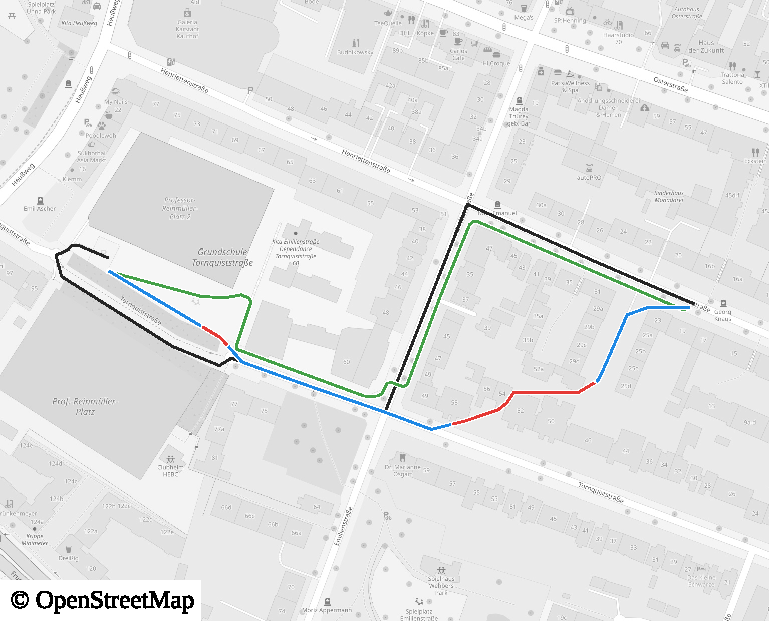
\includegraphics[width=0.65\textwidth]{../thesis/images/qgis-routing-city-routing-6.pdf}
				\end{figcenter}
				\caption{Expected (green), graph-based (black) and actual (blue) routes. Faulty passages marked in red.}
			\end{figure}
		\end{frame}
		
		\begin{frame}{Route quality analysis -- Example (OSM city)}
			\begin{figure}
				\begin{figcenter}
					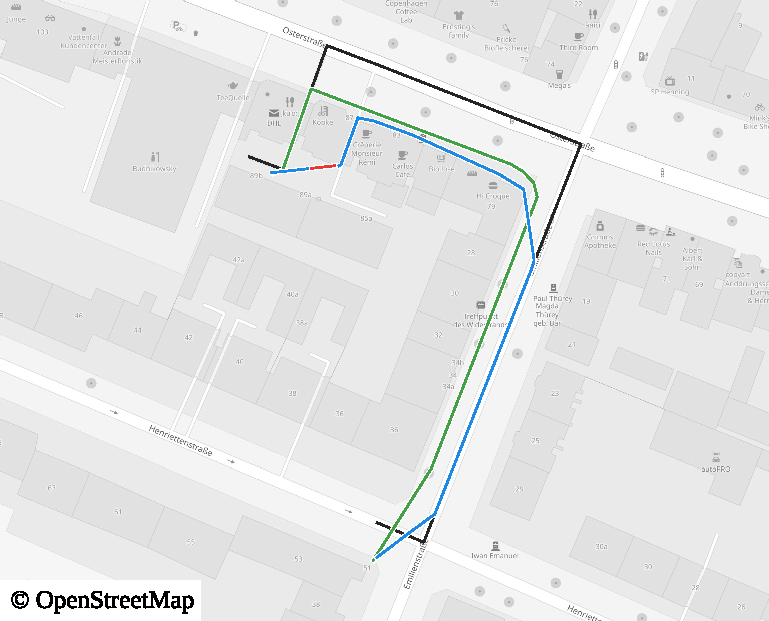
\includegraphics[width=0.65\textwidth]{../thesis/images/qgis-routing-city-routing-1.pdf}
				\end{figcenter}
				\caption{Expected (green), graph-based (black) and actual (blue) routes. Faulty passages marked in red.}
			\end{figure}
		\end{frame}
		
		\begin{frame}{Route quality analysis -- Example (OSM city)}
		\begin{figure}
			\begin{figcenter}
				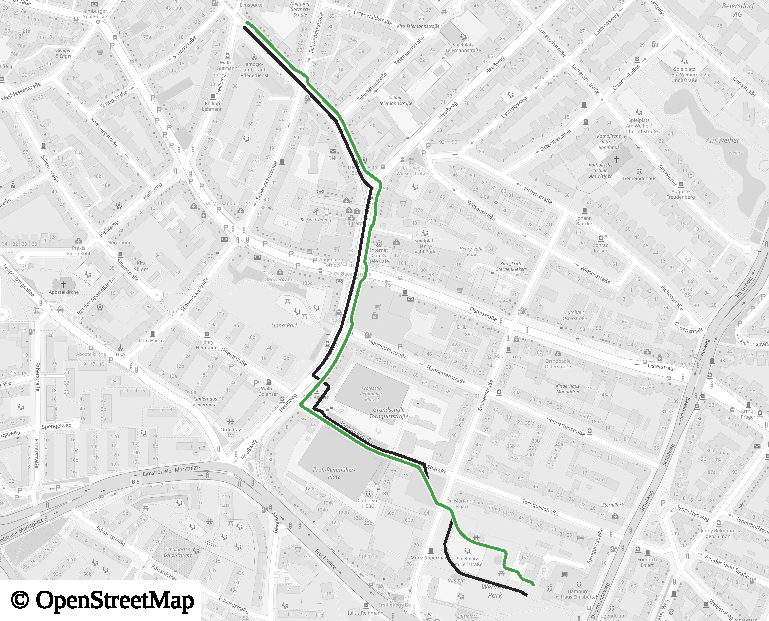
\includegraphics[width=0.65\textwidth]{images/qgis-routing-similar.pdf}
			\end{figcenter}
			\caption{Urban graph-based route (red) is already similar to expected route (green).}
		\end{figure}
		\end{frame}
		
		\begin{frame}{Route quality analysis -- Example (OSM rural)}
			\begin{figure}
				\begin{figcenter}
					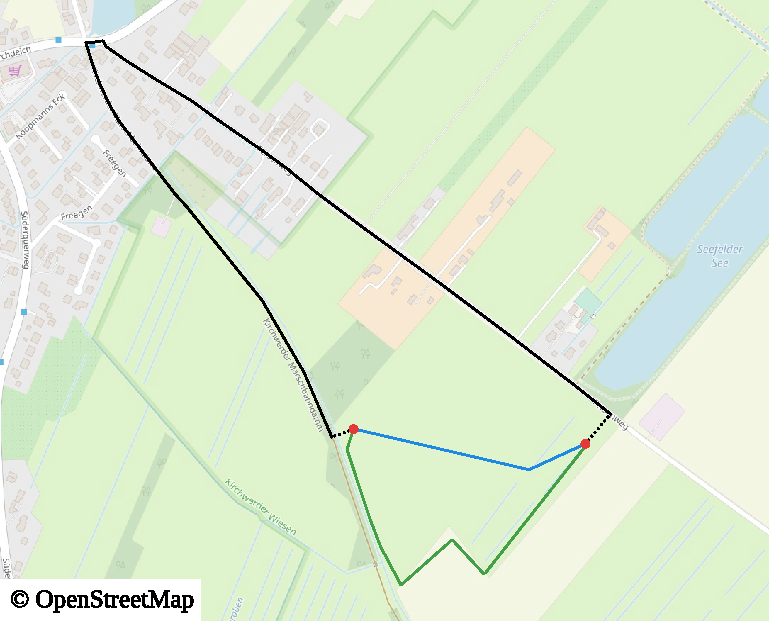
\includegraphics[width=0.65\textwidth]{images/qgis-routing-rural-routing-6-graph-based.pdf}
				\end{figcenter}
				\caption{Expected (green), graph-based (red) and actual (blue) routes.\newline\ }
			\end{figure}
		\end{frame}
		
		\begin{frame}{Hausdorff distances of routes}
			\begin{figure}
				\begin{figcenter}
					\scalebox{0.66}
					{
						%% Creator: Matplotlib, PGF backend
%%
%% To include the figure in your LaTeX document, write
%%   \input{<filename>.pgf}
%%
%% Make sure the required packages are loaded in your preamble
%%   \usepackage{pgf}
%%
%% Also ensure that all the required font packages are loaded; for instance,
%% the lmodern package is sometimes necessary when using math font.
%%   \usepackage{lmodern}
%%
%% Figures using additional raster images can only be included by \input if
%% they are in the same directory as the main LaTeX file. For loading figures
%% from other directories you can use the `import` package
%%   \usepackage{import}
%%
%% and then include the figures with
%%   \import{<path to file>}{<filename>.pgf}
%%
%% Matplotlib used the following preamble
%%   
%%   \usepackage{fontspec}
%%   \setmainfont{DejaVuSerif.ttf}[Path=\detokenize{/home/hauke/.local/lib/python3.11/site-packages/matplotlib/mpl-data/fonts/ttf/}]
%%   \setsansfont{DroidSans.ttf}[Path=\detokenize{/usr/share/fonts/droid/}]
%%   \setmonofont{DejaVuSansMono.ttf}[Path=\detokenize{/home/hauke/.local/lib/python3.11/site-packages/matplotlib/mpl-data/fonts/ttf/}]
%%   \makeatletter\@ifpackageloaded{underscore}{}{\usepackage[strings]{underscore}}\makeatother
%%
\begingroup%
\makeatletter%
\begin{pgfpicture}%
\pgfpathrectangle{\pgfpointorigin}{\pgfqpoint{6.084564in}{1.715788in}}%
\pgfusepath{use as bounding box, clip}%
\begin{pgfscope}%
\pgfsetbuttcap%
\pgfsetmiterjoin%
\definecolor{currentfill}{rgb}{1.000000,1.000000,1.000000}%
\pgfsetfillcolor{currentfill}%
\pgfsetlinewidth{0.000000pt}%
\definecolor{currentstroke}{rgb}{1.000000,1.000000,1.000000}%
\pgfsetstrokecolor{currentstroke}%
\pgfsetdash{}{0pt}%
\pgfpathmoveto{\pgfqpoint{0.000000in}{0.000000in}}%
\pgfpathlineto{\pgfqpoint{6.084564in}{0.000000in}}%
\pgfpathlineto{\pgfqpoint{6.084564in}{1.715788in}}%
\pgfpathlineto{\pgfqpoint{0.000000in}{1.715788in}}%
\pgfpathlineto{\pgfqpoint{0.000000in}{0.000000in}}%
\pgfpathclose%
\pgfusepath{fill}%
\end{pgfscope}%
\begin{pgfscope}%
\pgfsetbuttcap%
\pgfsetmiterjoin%
\definecolor{currentfill}{rgb}{1.000000,1.000000,1.000000}%
\pgfsetfillcolor{currentfill}%
\pgfsetlinewidth{0.000000pt}%
\definecolor{currentstroke}{rgb}{0.000000,0.000000,0.000000}%
\pgfsetstrokecolor{currentstroke}%
\pgfsetstrokeopacity{0.000000}%
\pgfsetdash{}{0pt}%
\pgfpathmoveto{\pgfqpoint{0.532932in}{0.451389in}}%
\pgfpathlineto{\pgfqpoint{4.916693in}{0.451389in}}%
\pgfpathlineto{\pgfqpoint{4.916693in}{1.715788in}}%
\pgfpathlineto{\pgfqpoint{0.532932in}{1.715788in}}%
\pgfpathlineto{\pgfqpoint{0.532932in}{0.451389in}}%
\pgfpathclose%
\pgfusepath{fill}%
\end{pgfscope}%
\begin{pgfscope}%
\definecolor{textcolor}{rgb}{0.150000,0.150000,0.150000}%
\pgfsetstrokecolor{textcolor}%
\pgfsetfillcolor{textcolor}%
\pgftext[x=0.732194in,y=0.319444in,,top]{\color{textcolor}\sffamily\fontsize{9.000000}{10.800000}\selectfont 1}%
\end{pgfscope}%
\begin{pgfscope}%
\definecolor{textcolor}{rgb}{0.150000,0.150000,0.150000}%
\pgfsetstrokecolor{textcolor}%
\pgfsetfillcolor{textcolor}%
\pgftext[x=1.130717in,y=0.319444in,,top]{\color{textcolor}\sffamily\fontsize{9.000000}{10.800000}\selectfont 2}%
\end{pgfscope}%
\begin{pgfscope}%
\definecolor{textcolor}{rgb}{0.150000,0.150000,0.150000}%
\pgfsetstrokecolor{textcolor}%
\pgfsetfillcolor{textcolor}%
\pgftext[x=1.529241in,y=0.319444in,,top]{\color{textcolor}\sffamily\fontsize{9.000000}{10.800000}\selectfont 3}%
\end{pgfscope}%
\begin{pgfscope}%
\definecolor{textcolor}{rgb}{0.150000,0.150000,0.150000}%
\pgfsetstrokecolor{textcolor}%
\pgfsetfillcolor{textcolor}%
\pgftext[x=1.927765in,y=0.319444in,,top]{\color{textcolor}\sffamily\fontsize{9.000000}{10.800000}\selectfont 4}%
\end{pgfscope}%
\begin{pgfscope}%
\definecolor{textcolor}{rgb}{0.150000,0.150000,0.150000}%
\pgfsetstrokecolor{textcolor}%
\pgfsetfillcolor{textcolor}%
\pgftext[x=2.326289in,y=0.319444in,,top]{\color{textcolor}\sffamily\fontsize{9.000000}{10.800000}\selectfont 5}%
\end{pgfscope}%
\begin{pgfscope}%
\definecolor{textcolor}{rgb}{0.150000,0.150000,0.150000}%
\pgfsetstrokecolor{textcolor}%
\pgfsetfillcolor{textcolor}%
\pgftext[x=2.724813in,y=0.319444in,,top]{\color{textcolor}\sffamily\fontsize{9.000000}{10.800000}\selectfont 6}%
\end{pgfscope}%
\begin{pgfscope}%
\definecolor{textcolor}{rgb}{0.150000,0.150000,0.150000}%
\pgfsetstrokecolor{textcolor}%
\pgfsetfillcolor{textcolor}%
\pgftext[x=3.123336in,y=0.319444in,,top]{\color{textcolor}\sffamily\fontsize{9.000000}{10.800000}\selectfont 7}%
\end{pgfscope}%
\begin{pgfscope}%
\definecolor{textcolor}{rgb}{0.150000,0.150000,0.150000}%
\pgfsetstrokecolor{textcolor}%
\pgfsetfillcolor{textcolor}%
\pgftext[x=3.521860in,y=0.319444in,,top]{\color{textcolor}\sffamily\fontsize{9.000000}{10.800000}\selectfont 8}%
\end{pgfscope}%
\begin{pgfscope}%
\definecolor{textcolor}{rgb}{0.150000,0.150000,0.150000}%
\pgfsetstrokecolor{textcolor}%
\pgfsetfillcolor{textcolor}%
\pgftext[x=3.920384in,y=0.319444in,,top]{\color{textcolor}\sffamily\fontsize{9.000000}{10.800000}\selectfont 9}%
\end{pgfscope}%
\begin{pgfscope}%
\definecolor{textcolor}{rgb}{0.150000,0.150000,0.150000}%
\pgfsetstrokecolor{textcolor}%
\pgfsetfillcolor{textcolor}%
\pgftext[x=4.318908in,y=0.319444in,,top]{\color{textcolor}\sffamily\fontsize{9.000000}{10.800000}\selectfont 10}%
\end{pgfscope}%
\begin{pgfscope}%
\definecolor{textcolor}{rgb}{0.150000,0.150000,0.150000}%
\pgfsetstrokecolor{textcolor}%
\pgfsetfillcolor{textcolor}%
\pgftext[x=4.717432in,y=0.319444in,,top]{\color{textcolor}\sffamily\fontsize{9.000000}{10.800000}\selectfont mean}%
\end{pgfscope}%
\begin{pgfscope}%
\definecolor{textcolor}{rgb}{0.150000,0.150000,0.150000}%
\pgfsetstrokecolor{textcolor}%
\pgfsetfillcolor{textcolor}%
\pgftext[x=2.724813in,y=0.125000in,,top]{\color{textcolor}\sffamily\fontsize{9.000000}{10.800000}\selectfont Routing request}%
\end{pgfscope}%
\begin{pgfscope}%
\pgfpathrectangle{\pgfqpoint{0.532932in}{0.451389in}}{\pgfqpoint{4.383762in}{1.264399in}}%
\pgfusepath{clip}%
\pgfsetroundcap%
\pgfsetroundjoin%
\pgfsetlinewidth{1.003750pt}%
\definecolor{currentstroke}{rgb}{0.800000,0.800000,0.800000}%
\pgfsetstrokecolor{currentstroke}%
\pgfsetdash{}{0pt}%
\pgfpathmoveto{\pgfqpoint{0.532932in}{0.451389in}}%
\pgfpathlineto{\pgfqpoint{4.916693in}{0.451389in}}%
\pgfusepath{stroke}%
\end{pgfscope}%
\begin{pgfscope}%
\definecolor{textcolor}{rgb}{0.150000,0.150000,0.150000}%
\pgfsetstrokecolor{textcolor}%
\pgfsetfillcolor{textcolor}%
\pgftext[x=0.332140in, y=0.403903in, left, base]{\color{textcolor}\sffamily\fontsize{9.000000}{10.800000}\selectfont 0}%
\end{pgfscope}%
\begin{pgfscope}%
\pgfpathrectangle{\pgfqpoint{0.532932in}{0.451389in}}{\pgfqpoint{4.383762in}{1.264399in}}%
\pgfusepath{clip}%
\pgfsetroundcap%
\pgfsetroundjoin%
\pgfsetlinewidth{1.003750pt}%
\definecolor{currentstroke}{rgb}{0.800000,0.800000,0.800000}%
\pgfsetstrokecolor{currentstroke}%
\pgfsetdash{}{0pt}%
\pgfpathmoveto{\pgfqpoint{0.532932in}{0.884223in}}%
\pgfpathlineto{\pgfqpoint{4.916693in}{0.884223in}}%
\pgfusepath{stroke}%
\end{pgfscope}%
\begin{pgfscope}%
\definecolor{textcolor}{rgb}{0.150000,0.150000,0.150000}%
\pgfsetstrokecolor{textcolor}%
\pgfsetfillcolor{textcolor}%
\pgftext[x=0.194444in, y=0.836738in, left, base]{\color{textcolor}\sffamily\fontsize{9.000000}{10.800000}\selectfont 100}%
\end{pgfscope}%
\begin{pgfscope}%
\pgfpathrectangle{\pgfqpoint{0.532932in}{0.451389in}}{\pgfqpoint{4.383762in}{1.264399in}}%
\pgfusepath{clip}%
\pgfsetroundcap%
\pgfsetroundjoin%
\pgfsetlinewidth{1.003750pt}%
\definecolor{currentstroke}{rgb}{0.800000,0.800000,0.800000}%
\pgfsetstrokecolor{currentstroke}%
\pgfsetdash{}{0pt}%
\pgfpathmoveto{\pgfqpoint{0.532932in}{1.317058in}}%
\pgfpathlineto{\pgfqpoint{4.916693in}{1.317058in}}%
\pgfusepath{stroke}%
\end{pgfscope}%
\begin{pgfscope}%
\definecolor{textcolor}{rgb}{0.150000,0.150000,0.150000}%
\pgfsetstrokecolor{textcolor}%
\pgfsetfillcolor{textcolor}%
\pgftext[x=0.194444in, y=1.269573in, left, base]{\color{textcolor}\sffamily\fontsize{9.000000}{10.800000}\selectfont 200}%
\end{pgfscope}%
\begin{pgfscope}%
\definecolor{textcolor}{rgb}{0.150000,0.150000,0.150000}%
\pgfsetstrokecolor{textcolor}%
\pgfsetfillcolor{textcolor}%
\pgftext[x=0.125000in,y=1.083588in,,bottom,rotate=90.000000]{\color{textcolor}\sffamily\fontsize{9.000000}{10.800000}\selectfont Hausdorff distance}%
\end{pgfscope}%
\begin{pgfscope}%
\pgfpathrectangle{\pgfqpoint{0.532932in}{0.451389in}}{\pgfqpoint{4.383762in}{1.264399in}}%
\pgfusepath{clip}%
\pgfsetbuttcap%
\pgfsetmiterjoin%
\definecolor{currentfill}{rgb}{0.349020,0.490196,0.749020}%
\pgfsetfillcolor{currentfill}%
\pgfsetlinewidth{1.003750pt}%
\definecolor{currentstroke}{rgb}{1.000000,1.000000,1.000000}%
\pgfsetstrokecolor{currentstroke}%
\pgfsetdash{}{0pt}%
\pgfpathmoveto{\pgfqpoint{0.572784in}{0.451389in}}%
\pgfpathlineto{\pgfqpoint{0.732194in}{0.451389in}}%
\pgfpathlineto{\pgfqpoint{0.732194in}{0.511243in}}%
\pgfpathlineto{\pgfqpoint{0.572784in}{0.511243in}}%
\pgfpathlineto{\pgfqpoint{0.572784in}{0.451389in}}%
\pgfpathclose%
\pgfusepath{stroke,fill}%
\end{pgfscope}%
\begin{pgfscope}%
\pgfpathrectangle{\pgfqpoint{0.532932in}{0.451389in}}{\pgfqpoint{4.383762in}{1.264399in}}%
\pgfusepath{clip}%
\pgfsetbuttcap%
\pgfsetmiterjoin%
\definecolor{currentfill}{rgb}{0.349020,0.490196,0.749020}%
\pgfsetfillcolor{currentfill}%
\pgfsetlinewidth{1.003750pt}%
\definecolor{currentstroke}{rgb}{1.000000,1.000000,1.000000}%
\pgfsetstrokecolor{currentstroke}%
\pgfsetdash{}{0pt}%
\pgfpathmoveto{\pgfqpoint{0.971308in}{0.451389in}}%
\pgfpathlineto{\pgfqpoint{1.130717in}{0.451389in}}%
\pgfpathlineto{\pgfqpoint{1.130717in}{0.520923in}}%
\pgfpathlineto{\pgfqpoint{0.971308in}{0.520923in}}%
\pgfpathlineto{\pgfqpoint{0.971308in}{0.451389in}}%
\pgfpathclose%
\pgfusepath{stroke,fill}%
\end{pgfscope}%
\begin{pgfscope}%
\pgfpathrectangle{\pgfqpoint{0.532932in}{0.451389in}}{\pgfqpoint{4.383762in}{1.264399in}}%
\pgfusepath{clip}%
\pgfsetbuttcap%
\pgfsetmiterjoin%
\definecolor{currentfill}{rgb}{0.349020,0.490196,0.749020}%
\pgfsetfillcolor{currentfill}%
\pgfsetlinewidth{1.003750pt}%
\definecolor{currentstroke}{rgb}{1.000000,1.000000,1.000000}%
\pgfsetstrokecolor{currentstroke}%
\pgfsetdash{}{0pt}%
\pgfpathmoveto{\pgfqpoint{1.369832in}{0.451389in}}%
\pgfpathlineto{\pgfqpoint{1.529241in}{0.451389in}}%
\pgfpathlineto{\pgfqpoint{1.529241in}{0.720067in}}%
\pgfpathlineto{\pgfqpoint{1.369832in}{0.720067in}}%
\pgfpathlineto{\pgfqpoint{1.369832in}{0.451389in}}%
\pgfpathclose%
\pgfusepath{stroke,fill}%
\end{pgfscope}%
\begin{pgfscope}%
\pgfpathrectangle{\pgfqpoint{0.532932in}{0.451389in}}{\pgfqpoint{4.383762in}{1.264399in}}%
\pgfusepath{clip}%
\pgfsetbuttcap%
\pgfsetmiterjoin%
\definecolor{currentfill}{rgb}{0.349020,0.490196,0.749020}%
\pgfsetfillcolor{currentfill}%
\pgfsetlinewidth{1.003750pt}%
\definecolor{currentstroke}{rgb}{1.000000,1.000000,1.000000}%
\pgfsetstrokecolor{currentstroke}%
\pgfsetdash{}{0pt}%
\pgfpathmoveto{\pgfqpoint{1.768356in}{0.451389in}}%
\pgfpathlineto{\pgfqpoint{1.927765in}{0.451389in}}%
\pgfpathlineto{\pgfqpoint{1.927765in}{0.495508in}}%
\pgfpathlineto{\pgfqpoint{1.768356in}{0.495508in}}%
\pgfpathlineto{\pgfqpoint{1.768356in}{0.451389in}}%
\pgfpathclose%
\pgfusepath{stroke,fill}%
\end{pgfscope}%
\begin{pgfscope}%
\pgfpathrectangle{\pgfqpoint{0.532932in}{0.451389in}}{\pgfqpoint{4.383762in}{1.264399in}}%
\pgfusepath{clip}%
\pgfsetbuttcap%
\pgfsetmiterjoin%
\definecolor{currentfill}{rgb}{0.349020,0.490196,0.749020}%
\pgfsetfillcolor{currentfill}%
\pgfsetlinewidth{1.003750pt}%
\definecolor{currentstroke}{rgb}{1.000000,1.000000,1.000000}%
\pgfsetstrokecolor{currentstroke}%
\pgfsetdash{}{0pt}%
\pgfpathmoveto{\pgfqpoint{2.166879in}{0.451389in}}%
\pgfpathlineto{\pgfqpoint{2.326289in}{0.451389in}}%
\pgfpathlineto{\pgfqpoint{2.326289in}{0.995589in}}%
\pgfpathlineto{\pgfqpoint{2.166879in}{0.995589in}}%
\pgfpathlineto{\pgfqpoint{2.166879in}{0.451389in}}%
\pgfpathclose%
\pgfusepath{stroke,fill}%
\end{pgfscope}%
\begin{pgfscope}%
\pgfpathrectangle{\pgfqpoint{0.532932in}{0.451389in}}{\pgfqpoint{4.383762in}{1.264399in}}%
\pgfusepath{clip}%
\pgfsetbuttcap%
\pgfsetmiterjoin%
\definecolor{currentfill}{rgb}{0.349020,0.490196,0.749020}%
\pgfsetfillcolor{currentfill}%
\pgfsetlinewidth{1.003750pt}%
\definecolor{currentstroke}{rgb}{1.000000,1.000000,1.000000}%
\pgfsetstrokecolor{currentstroke}%
\pgfsetdash{}{0pt}%
\pgfpathmoveto{\pgfqpoint{2.565403in}{0.451389in}}%
\pgfpathlineto{\pgfqpoint{2.724813in}{0.451389in}}%
\pgfpathlineto{\pgfqpoint{2.724813in}{0.908684in}}%
\pgfpathlineto{\pgfqpoint{2.565403in}{0.908684in}}%
\pgfpathlineto{\pgfqpoint{2.565403in}{0.451389in}}%
\pgfpathclose%
\pgfusepath{stroke,fill}%
\end{pgfscope}%
\begin{pgfscope}%
\pgfpathrectangle{\pgfqpoint{0.532932in}{0.451389in}}{\pgfqpoint{4.383762in}{1.264399in}}%
\pgfusepath{clip}%
\pgfsetbuttcap%
\pgfsetmiterjoin%
\definecolor{currentfill}{rgb}{0.349020,0.490196,0.749020}%
\pgfsetfillcolor{currentfill}%
\pgfsetlinewidth{1.003750pt}%
\definecolor{currentstroke}{rgb}{1.000000,1.000000,1.000000}%
\pgfsetstrokecolor{currentstroke}%
\pgfsetdash{}{0pt}%
\pgfpathmoveto{\pgfqpoint{2.963927in}{0.451389in}}%
\pgfpathlineto{\pgfqpoint{3.123336in}{0.451389in}}%
\pgfpathlineto{\pgfqpoint{3.123336in}{0.578894in}}%
\pgfpathlineto{\pgfqpoint{2.963927in}{0.578894in}}%
\pgfpathlineto{\pgfqpoint{2.963927in}{0.451389in}}%
\pgfpathclose%
\pgfusepath{stroke,fill}%
\end{pgfscope}%
\begin{pgfscope}%
\pgfpathrectangle{\pgfqpoint{0.532932in}{0.451389in}}{\pgfqpoint{4.383762in}{1.264399in}}%
\pgfusepath{clip}%
\pgfsetbuttcap%
\pgfsetmiterjoin%
\definecolor{currentfill}{rgb}{0.349020,0.490196,0.749020}%
\pgfsetfillcolor{currentfill}%
\pgfsetlinewidth{1.003750pt}%
\definecolor{currentstroke}{rgb}{1.000000,1.000000,1.000000}%
\pgfsetstrokecolor{currentstroke}%
\pgfsetdash{}{0pt}%
\pgfpathmoveto{\pgfqpoint{3.362451in}{0.451389in}}%
\pgfpathlineto{\pgfqpoint{3.521860in}{0.451389in}}%
\pgfpathlineto{\pgfqpoint{3.521860in}{0.916688in}}%
\pgfpathlineto{\pgfqpoint{3.362451in}{0.916688in}}%
\pgfpathlineto{\pgfqpoint{3.362451in}{0.451389in}}%
\pgfpathclose%
\pgfusepath{stroke,fill}%
\end{pgfscope}%
\begin{pgfscope}%
\pgfpathrectangle{\pgfqpoint{0.532932in}{0.451389in}}{\pgfqpoint{4.383762in}{1.264399in}}%
\pgfusepath{clip}%
\pgfsetbuttcap%
\pgfsetmiterjoin%
\definecolor{currentfill}{rgb}{0.349020,0.490196,0.749020}%
\pgfsetfillcolor{currentfill}%
\pgfsetlinewidth{1.003750pt}%
\definecolor{currentstroke}{rgb}{1.000000,1.000000,1.000000}%
\pgfsetstrokecolor{currentstroke}%
\pgfsetdash{}{0pt}%
\pgfpathmoveto{\pgfqpoint{3.760974in}{0.451389in}}%
\pgfpathlineto{\pgfqpoint{3.920384in}{0.451389in}}%
\pgfpathlineto{\pgfqpoint{3.920384in}{0.646408in}}%
\pgfpathlineto{\pgfqpoint{3.760974in}{0.646408in}}%
\pgfpathlineto{\pgfqpoint{3.760974in}{0.451389in}}%
\pgfpathclose%
\pgfusepath{stroke,fill}%
\end{pgfscope}%
\begin{pgfscope}%
\pgfpathrectangle{\pgfqpoint{0.532932in}{0.451389in}}{\pgfqpoint{4.383762in}{1.264399in}}%
\pgfusepath{clip}%
\pgfsetbuttcap%
\pgfsetmiterjoin%
\definecolor{currentfill}{rgb}{0.349020,0.490196,0.749020}%
\pgfsetfillcolor{currentfill}%
\pgfsetlinewidth{1.003750pt}%
\definecolor{currentstroke}{rgb}{1.000000,1.000000,1.000000}%
\pgfsetstrokecolor{currentstroke}%
\pgfsetdash{}{0pt}%
\pgfpathmoveto{\pgfqpoint{4.159498in}{0.451389in}}%
\pgfpathlineto{\pgfqpoint{4.318908in}{0.451389in}}%
\pgfpathlineto{\pgfqpoint{4.318908in}{1.148726in}}%
\pgfpathlineto{\pgfqpoint{4.159498in}{1.148726in}}%
\pgfpathlineto{\pgfqpoint{4.159498in}{0.451389in}}%
\pgfpathclose%
\pgfusepath{stroke,fill}%
\end{pgfscope}%
\begin{pgfscope}%
\pgfpathrectangle{\pgfqpoint{0.532932in}{0.451389in}}{\pgfqpoint{4.383762in}{1.264399in}}%
\pgfusepath{clip}%
\pgfsetbuttcap%
\pgfsetmiterjoin%
\definecolor{currentfill}{rgb}{0.349020,0.490196,0.749020}%
\pgfsetfillcolor{currentfill}%
\pgfsetlinewidth{1.003750pt}%
\definecolor{currentstroke}{rgb}{1.000000,1.000000,1.000000}%
\pgfsetstrokecolor{currentstroke}%
\pgfsetdash{}{0pt}%
\pgfpathmoveto{\pgfqpoint{4.558022in}{0.451389in}}%
\pgfpathlineto{\pgfqpoint{4.717432in}{0.451389in}}%
\pgfpathlineto{\pgfqpoint{4.717432in}{0.744273in}}%
\pgfpathlineto{\pgfqpoint{4.558022in}{0.744273in}}%
\pgfpathlineto{\pgfqpoint{4.558022in}{0.451389in}}%
\pgfpathclose%
\pgfusepath{stroke,fill}%
\end{pgfscope}%
\begin{pgfscope}%
\pgfpathrectangle{\pgfqpoint{0.532932in}{0.451389in}}{\pgfqpoint{4.383762in}{1.264399in}}%
\pgfusepath{clip}%
\pgfsetbuttcap%
\pgfsetmiterjoin%
\definecolor{currentfill}{rgb}{0.852941,0.544118,0.370588}%
\pgfsetfillcolor{currentfill}%
\pgfsetlinewidth{1.003750pt}%
\definecolor{currentstroke}{rgb}{1.000000,1.000000,1.000000}%
\pgfsetstrokecolor{currentstroke}%
\pgfsetdash{}{0pt}%
\pgfpathmoveto{\pgfqpoint{0.732194in}{0.451389in}}%
\pgfpathlineto{\pgfqpoint{0.891603in}{0.451389in}}%
\pgfpathlineto{\pgfqpoint{0.891603in}{0.517848in}}%
\pgfpathlineto{\pgfqpoint{0.732194in}{0.517848in}}%
\pgfpathlineto{\pgfqpoint{0.732194in}{0.451389in}}%
\pgfpathclose%
\pgfusepath{stroke,fill}%
\end{pgfscope}%
\begin{pgfscope}%
\pgfpathrectangle{\pgfqpoint{0.532932in}{0.451389in}}{\pgfqpoint{4.383762in}{1.264399in}}%
\pgfusepath{clip}%
\pgfsetbuttcap%
\pgfsetmiterjoin%
\definecolor{currentfill}{rgb}{0.852941,0.544118,0.370588}%
\pgfsetfillcolor{currentfill}%
\pgfsetlinewidth{1.003750pt}%
\definecolor{currentstroke}{rgb}{1.000000,1.000000,1.000000}%
\pgfsetstrokecolor{currentstroke}%
\pgfsetdash{}{0pt}%
\pgfpathmoveto{\pgfqpoint{1.130717in}{0.451389in}}%
\pgfpathlineto{\pgfqpoint{1.290127in}{0.451389in}}%
\pgfpathlineto{\pgfqpoint{1.290127in}{0.570385in}}%
\pgfpathlineto{\pgfqpoint{1.130717in}{0.570385in}}%
\pgfpathlineto{\pgfqpoint{1.130717in}{0.451389in}}%
\pgfpathclose%
\pgfusepath{stroke,fill}%
\end{pgfscope}%
\begin{pgfscope}%
\pgfpathrectangle{\pgfqpoint{0.532932in}{0.451389in}}{\pgfqpoint{4.383762in}{1.264399in}}%
\pgfusepath{clip}%
\pgfsetbuttcap%
\pgfsetmiterjoin%
\definecolor{currentfill}{rgb}{0.852941,0.544118,0.370588}%
\pgfsetfillcolor{currentfill}%
\pgfsetlinewidth{1.003750pt}%
\definecolor{currentstroke}{rgb}{1.000000,1.000000,1.000000}%
\pgfsetstrokecolor{currentstroke}%
\pgfsetdash{}{0pt}%
\pgfpathmoveto{\pgfqpoint{1.529241in}{0.451389in}}%
\pgfpathlineto{\pgfqpoint{1.688651in}{0.451389in}}%
\pgfpathlineto{\pgfqpoint{1.688651in}{0.544182in}}%
\pgfpathlineto{\pgfqpoint{1.529241in}{0.544182in}}%
\pgfpathlineto{\pgfqpoint{1.529241in}{0.451389in}}%
\pgfpathclose%
\pgfusepath{stroke,fill}%
\end{pgfscope}%
\begin{pgfscope}%
\pgfpathrectangle{\pgfqpoint{0.532932in}{0.451389in}}{\pgfqpoint{4.383762in}{1.264399in}}%
\pgfusepath{clip}%
\pgfsetbuttcap%
\pgfsetmiterjoin%
\definecolor{currentfill}{rgb}{0.852941,0.544118,0.370588}%
\pgfsetfillcolor{currentfill}%
\pgfsetlinewidth{1.003750pt}%
\definecolor{currentstroke}{rgb}{1.000000,1.000000,1.000000}%
\pgfsetstrokecolor{currentstroke}%
\pgfsetdash{}{0pt}%
\pgfpathmoveto{\pgfqpoint{1.927765in}{0.451389in}}%
\pgfpathlineto{\pgfqpoint{2.087175in}{0.451389in}}%
\pgfpathlineto{\pgfqpoint{2.087175in}{0.498410in}}%
\pgfpathlineto{\pgfqpoint{1.927765in}{0.498410in}}%
\pgfpathlineto{\pgfqpoint{1.927765in}{0.451389in}}%
\pgfpathclose%
\pgfusepath{stroke,fill}%
\end{pgfscope}%
\begin{pgfscope}%
\pgfpathrectangle{\pgfqpoint{0.532932in}{0.451389in}}{\pgfqpoint{4.383762in}{1.264399in}}%
\pgfusepath{clip}%
\pgfsetbuttcap%
\pgfsetmiterjoin%
\definecolor{currentfill}{rgb}{0.852941,0.544118,0.370588}%
\pgfsetfillcolor{currentfill}%
\pgfsetlinewidth{1.003750pt}%
\definecolor{currentstroke}{rgb}{1.000000,1.000000,1.000000}%
\pgfsetstrokecolor{currentstroke}%
\pgfsetdash{}{0pt}%
\pgfpathmoveto{\pgfqpoint{2.326289in}{0.451389in}}%
\pgfpathlineto{\pgfqpoint{2.485698in}{0.451389in}}%
\pgfpathlineto{\pgfqpoint{2.485698in}{1.369560in}}%
\pgfpathlineto{\pgfqpoint{2.326289in}{1.369560in}}%
\pgfpathlineto{\pgfqpoint{2.326289in}{0.451389in}}%
\pgfpathclose%
\pgfusepath{stroke,fill}%
\end{pgfscope}%
\begin{pgfscope}%
\pgfpathrectangle{\pgfqpoint{0.532932in}{0.451389in}}{\pgfqpoint{4.383762in}{1.264399in}}%
\pgfusepath{clip}%
\pgfsetbuttcap%
\pgfsetmiterjoin%
\definecolor{currentfill}{rgb}{0.852941,0.544118,0.370588}%
\pgfsetfillcolor{currentfill}%
\pgfsetlinewidth{1.003750pt}%
\definecolor{currentstroke}{rgb}{1.000000,1.000000,1.000000}%
\pgfsetstrokecolor{currentstroke}%
\pgfsetdash{}{0pt}%
\pgfpathmoveto{\pgfqpoint{2.724813in}{0.451389in}}%
\pgfpathlineto{\pgfqpoint{2.884222in}{0.451389in}}%
\pgfpathlineto{\pgfqpoint{2.884222in}{0.619132in}}%
\pgfpathlineto{\pgfqpoint{2.724813in}{0.619132in}}%
\pgfpathlineto{\pgfqpoint{2.724813in}{0.451389in}}%
\pgfpathclose%
\pgfusepath{stroke,fill}%
\end{pgfscope}%
\begin{pgfscope}%
\pgfpathrectangle{\pgfqpoint{0.532932in}{0.451389in}}{\pgfqpoint{4.383762in}{1.264399in}}%
\pgfusepath{clip}%
\pgfsetbuttcap%
\pgfsetmiterjoin%
\definecolor{currentfill}{rgb}{0.852941,0.544118,0.370588}%
\pgfsetfillcolor{currentfill}%
\pgfsetlinewidth{1.003750pt}%
\definecolor{currentstroke}{rgb}{1.000000,1.000000,1.000000}%
\pgfsetstrokecolor{currentstroke}%
\pgfsetdash{}{0pt}%
\pgfpathmoveto{\pgfqpoint{3.123336in}{0.451389in}}%
\pgfpathlineto{\pgfqpoint{3.282746in}{0.451389in}}%
\pgfpathlineto{\pgfqpoint{3.282746in}{0.619132in}}%
\pgfpathlineto{\pgfqpoint{3.123336in}{0.619132in}}%
\pgfpathlineto{\pgfqpoint{3.123336in}{0.451389in}}%
\pgfpathclose%
\pgfusepath{stroke,fill}%
\end{pgfscope}%
\begin{pgfscope}%
\pgfpathrectangle{\pgfqpoint{0.532932in}{0.451389in}}{\pgfqpoint{4.383762in}{1.264399in}}%
\pgfusepath{clip}%
\pgfsetbuttcap%
\pgfsetmiterjoin%
\definecolor{currentfill}{rgb}{0.852941,0.544118,0.370588}%
\pgfsetfillcolor{currentfill}%
\pgfsetlinewidth{1.003750pt}%
\definecolor{currentstroke}{rgb}{1.000000,1.000000,1.000000}%
\pgfsetstrokecolor{currentstroke}%
\pgfsetdash{}{0pt}%
\pgfpathmoveto{\pgfqpoint{3.521860in}{0.451389in}}%
\pgfpathlineto{\pgfqpoint{3.681270in}{0.451389in}}%
\pgfpathlineto{\pgfqpoint{3.681270in}{1.140506in}}%
\pgfpathlineto{\pgfqpoint{3.521860in}{1.140506in}}%
\pgfpathlineto{\pgfqpoint{3.521860in}{0.451389in}}%
\pgfpathclose%
\pgfusepath{stroke,fill}%
\end{pgfscope}%
\begin{pgfscope}%
\pgfpathrectangle{\pgfqpoint{0.532932in}{0.451389in}}{\pgfqpoint{4.383762in}{1.264399in}}%
\pgfusepath{clip}%
\pgfsetbuttcap%
\pgfsetmiterjoin%
\definecolor{currentfill}{rgb}{0.852941,0.544118,0.370588}%
\pgfsetfillcolor{currentfill}%
\pgfsetlinewidth{1.003750pt}%
\definecolor{currentstroke}{rgb}{1.000000,1.000000,1.000000}%
\pgfsetstrokecolor{currentstroke}%
\pgfsetdash{}{0pt}%
\pgfpathmoveto{\pgfqpoint{3.920384in}{0.451389in}}%
\pgfpathlineto{\pgfqpoint{4.079794in}{0.451389in}}%
\pgfpathlineto{\pgfqpoint{4.079794in}{0.564899in}}%
\pgfpathlineto{\pgfqpoint{3.920384in}{0.564899in}}%
\pgfpathlineto{\pgfqpoint{3.920384in}{0.451389in}}%
\pgfpathclose%
\pgfusepath{stroke,fill}%
\end{pgfscope}%
\begin{pgfscope}%
\pgfpathrectangle{\pgfqpoint{0.532932in}{0.451389in}}{\pgfqpoint{4.383762in}{1.264399in}}%
\pgfusepath{clip}%
\pgfsetbuttcap%
\pgfsetmiterjoin%
\definecolor{currentfill}{rgb}{0.852941,0.544118,0.370588}%
\pgfsetfillcolor{currentfill}%
\pgfsetlinewidth{1.003750pt}%
\definecolor{currentstroke}{rgb}{1.000000,1.000000,1.000000}%
\pgfsetstrokecolor{currentstroke}%
\pgfsetdash{}{0pt}%
\pgfpathmoveto{\pgfqpoint{4.318908in}{0.451389in}}%
\pgfpathlineto{\pgfqpoint{4.478317in}{0.451389in}}%
\pgfpathlineto{\pgfqpoint{4.478317in}{1.655578in}}%
\pgfpathlineto{\pgfqpoint{4.318908in}{1.655578in}}%
\pgfpathlineto{\pgfqpoint{4.318908in}{0.451389in}}%
\pgfpathclose%
\pgfusepath{stroke,fill}%
\end{pgfscope}%
\begin{pgfscope}%
\pgfpathrectangle{\pgfqpoint{0.532932in}{0.451389in}}{\pgfqpoint{4.383762in}{1.264399in}}%
\pgfusepath{clip}%
\pgfsetbuttcap%
\pgfsetmiterjoin%
\definecolor{currentfill}{rgb}{0.852941,0.544118,0.370588}%
\pgfsetfillcolor{currentfill}%
\pgfsetlinewidth{1.003750pt}%
\definecolor{currentstroke}{rgb}{1.000000,1.000000,1.000000}%
\pgfsetstrokecolor{currentstroke}%
\pgfsetdash{}{0pt}%
\pgfpathmoveto{\pgfqpoint{4.717432in}{0.451389in}}%
\pgfpathlineto{\pgfqpoint{4.876841in}{0.451389in}}%
\pgfpathlineto{\pgfqpoint{4.876841in}{0.809963in}}%
\pgfpathlineto{\pgfqpoint{4.717432in}{0.809963in}}%
\pgfpathlineto{\pgfqpoint{4.717432in}{0.451389in}}%
\pgfpathclose%
\pgfusepath{stroke,fill}%
\end{pgfscope}%
\begin{pgfscope}%
\pgfsetrectcap%
\pgfsetmiterjoin%
\pgfsetlinewidth{1.254687pt}%
\definecolor{currentstroke}{rgb}{0.800000,0.800000,0.800000}%
\pgfsetstrokecolor{currentstroke}%
\pgfsetdash{}{0pt}%
\pgfpathmoveto{\pgfqpoint{0.532932in}{0.451389in}}%
\pgfpathlineto{\pgfqpoint{0.532932in}{1.715788in}}%
\pgfusepath{stroke}%
\end{pgfscope}%
\begin{pgfscope}%
\pgfsetrectcap%
\pgfsetmiterjoin%
\pgfsetlinewidth{1.254687pt}%
\definecolor{currentstroke}{rgb}{0.800000,0.800000,0.800000}%
\pgfsetstrokecolor{currentstroke}%
\pgfsetdash{}{0pt}%
\pgfpathmoveto{\pgfqpoint{4.916693in}{0.451389in}}%
\pgfpathlineto{\pgfqpoint{4.916693in}{1.715788in}}%
\pgfusepath{stroke}%
\end{pgfscope}%
\begin{pgfscope}%
\pgfsetrectcap%
\pgfsetmiterjoin%
\pgfsetlinewidth{1.254687pt}%
\definecolor{currentstroke}{rgb}{0.800000,0.800000,0.800000}%
\pgfsetstrokecolor{currentstroke}%
\pgfsetdash{}{0pt}%
\pgfpathmoveto{\pgfqpoint{0.532932in}{0.451389in}}%
\pgfpathlineto{\pgfqpoint{4.916693in}{0.451389in}}%
\pgfusepath{stroke}%
\end{pgfscope}%
\begin{pgfscope}%
\pgfsetrectcap%
\pgfsetmiterjoin%
\pgfsetlinewidth{1.254687pt}%
\definecolor{currentstroke}{rgb}{0.800000,0.800000,0.800000}%
\pgfsetstrokecolor{currentstroke}%
\pgfsetdash{}{0pt}%
\pgfpathmoveto{\pgfqpoint{0.532932in}{1.715788in}}%
\pgfpathlineto{\pgfqpoint{4.916693in}{1.715788in}}%
\pgfusepath{stroke}%
\end{pgfscope}%
\begin{pgfscope}%
\pgfsetbuttcap%
\pgfsetmiterjoin%
\definecolor{currentfill}{rgb}{1.000000,1.000000,1.000000}%
\pgfsetfillcolor{currentfill}%
\pgfsetfillopacity{0.800000}%
\pgfsetlinewidth{1.003750pt}%
\definecolor{currentstroke}{rgb}{0.800000,0.800000,0.800000}%
\pgfsetstrokecolor{currentstroke}%
\pgfsetstrokeopacity{0.800000}%
\pgfsetdash{}{0pt}%
\pgfpathmoveto{\pgfqpoint{5.113788in}{0.589350in}}%
\pgfpathlineto{\pgfqpoint{6.059564in}{0.589350in}}%
\pgfpathquadraticcurveto{\pgfqpoint{6.084564in}{0.589350in}}{\pgfqpoint{6.084564in}{0.614350in}}%
\pgfpathlineto{\pgfqpoint{6.084564in}{1.552826in}}%
\pgfpathquadraticcurveto{\pgfqpoint{6.084564in}{1.577826in}}{\pgfqpoint{6.059564in}{1.577826in}}%
\pgfpathlineto{\pgfqpoint{5.113788in}{1.577826in}}%
\pgfpathquadraticcurveto{\pgfqpoint{5.088788in}{1.577826in}}{\pgfqpoint{5.088788in}{1.552826in}}%
\pgfpathlineto{\pgfqpoint{5.088788in}{0.614350in}}%
\pgfpathquadraticcurveto{\pgfqpoint{5.088788in}{0.589350in}}{\pgfqpoint{5.113788in}{0.589350in}}%
\pgfpathlineto{\pgfqpoint{5.113788in}{0.589350in}}%
\pgfpathclose%
\pgfusepath{stroke,fill}%
\end{pgfscope}%
\begin{pgfscope}%
\pgfsetbuttcap%
\pgfsetmiterjoin%
\definecolor{currentfill}{rgb}{0.349020,0.490196,0.749020}%
\pgfsetfillcolor{currentfill}%
\pgfsetlinewidth{1.003750pt}%
\definecolor{currentstroke}{rgb}{1.000000,1.000000,1.000000}%
\pgfsetstrokecolor{currentstroke}%
\pgfsetdash{}{0pt}%
\pgfpathmoveto{\pgfqpoint{5.138788in}{1.273847in}}%
\pgfpathlineto{\pgfqpoint{5.388788in}{1.273847in}}%
\pgfpathlineto{\pgfqpoint{5.388788in}{1.361347in}}%
\pgfpathlineto{\pgfqpoint{5.138788in}{1.361347in}}%
\pgfpathlineto{\pgfqpoint{5.138788in}{1.273847in}}%
\pgfpathclose%
\pgfusepath{stroke,fill}%
\end{pgfscope}%
\begin{pgfscope}%
\definecolor{textcolor}{rgb}{0.150000,0.150000,0.150000}%
\pgfsetstrokecolor{textcolor}%
\pgfsetfillcolor{textcolor}%
\pgftext[x=5.488788in, y=1.432855in, left, base]{\color{textcolor}\sffamily\fontsize{9.000000}{10.800000}\selectfont Hybrid}%
\end{pgfscope}%
\begin{pgfscope}%
\definecolor{textcolor}{rgb}{0.150000,0.150000,0.150000}%
\pgfsetstrokecolor{textcolor}%
\pgfsetfillcolor{textcolor}%
\pgftext[x=5.488788in, y=1.288861in, left, base]{\color{textcolor}\sffamily\fontsize{9.000000}{10.800000}\selectfont routing}%
\end{pgfscope}%
\begin{pgfscope}%
\definecolor{textcolor}{rgb}{0.150000,0.150000,0.150000}%
\pgfsetstrokecolor{textcolor}%
\pgfsetfillcolor{textcolor}%
\pgftext[x=5.488788in, y=1.144867in, left, base]{\color{textcolor}\sffamily\fontsize{9.000000}{10.800000}\selectfont algorithm}%
\end{pgfscope}%
\begin{pgfscope}%
\pgfsetbuttcap%
\pgfsetmiterjoin%
\definecolor{currentfill}{rgb}{0.852941,0.544118,0.370588}%
\pgfsetfillcolor{currentfill}%
\pgfsetlinewidth{1.003750pt}%
\definecolor{currentstroke}{rgb}{1.000000,1.000000,1.000000}%
\pgfsetstrokecolor{currentstroke}%
\pgfsetdash{}{0pt}%
\pgfpathmoveto{\pgfqpoint{5.138788in}{0.798359in}}%
\pgfpathlineto{\pgfqpoint{5.388788in}{0.798359in}}%
\pgfpathlineto{\pgfqpoint{5.388788in}{0.885859in}}%
\pgfpathlineto{\pgfqpoint{5.138788in}{0.885859in}}%
\pgfpathlineto{\pgfqpoint{5.138788in}{0.798359in}}%
\pgfpathclose%
\pgfusepath{stroke,fill}%
\end{pgfscope}%
\begin{pgfscope}%
\definecolor{textcolor}{rgb}{0.150000,0.150000,0.150000}%
\pgfsetstrokecolor{textcolor}%
\pgfsetfillcolor{textcolor}%
\pgftext[x=5.488788in, y=0.957367in, left, base]{\color{textcolor}\sffamily\fontsize{9.000000}{10.800000}\selectfont Graph-}%
\end{pgfscope}%
\begin{pgfscope}%
\definecolor{textcolor}{rgb}{0.150000,0.150000,0.150000}%
\pgfsetstrokecolor{textcolor}%
\pgfsetfillcolor{textcolor}%
\pgftext[x=5.488788in, y=0.813373in, left, base]{\color{textcolor}\sffamily\fontsize{9.000000}{10.800000}\selectfont based}%
\end{pgfscope}%
\begin{pgfscope}%
\definecolor{textcolor}{rgb}{0.150000,0.150000,0.150000}%
\pgfsetstrokecolor{textcolor}%
\pgfsetfillcolor{textcolor}%
\pgftext[x=5.488788in, y=0.669379in, left, base]{\color{textcolor}\sffamily\fontsize{9.000000}{10.800000}\selectfont routing}%
\end{pgfscope}%
\end{pgfpicture}%
\makeatother%
\endgroup%

					}
					\scalebox{0.66}
					{
						%% Creator: Matplotlib, PGF backend
%%
%% To include the figure in your LaTeX document, write
%%   \input{<filename>.pgf}
%%
%% Make sure the required packages are loaded in your preamble
%%   \usepackage{pgf}
%%
%% Also ensure that all the required font packages are loaded; for instance,
%% the lmodern package is sometimes necessary when using math font.
%%   \usepackage{lmodern}
%%
%% Figures using additional raster images can only be included by \input if
%% they are in the same directory as the main LaTeX file. For loading figures
%% from other directories you can use the `import` package
%%   \usepackage{import}
%%
%% and then include the figures with
%%   \import{<path to file>}{<filename>.pgf}
%%
%% Matplotlib used the following preamble
%%   
%%   \usepackage{fontspec}
%%   \setmainfont{DejaVuSerif.ttf}[Path=\detokenize{/home/hauke/.local/lib/python3.11/site-packages/matplotlib/mpl-data/fonts/ttf/}]
%%   \setsansfont{DroidSans.ttf}[Path=\detokenize{/usr/share/fonts/droid/}]
%%   \setmonofont{DejaVuSansMono.ttf}[Path=\detokenize{/home/hauke/.local/lib/python3.11/site-packages/matplotlib/mpl-data/fonts/ttf/}]
%%   \makeatletter\@ifpackageloaded{underscore}{}{\usepackage[strings]{underscore}}\makeatother
%%
\begingroup%
\makeatletter%
\begin{pgfpicture}%
\pgfpathrectangle{\pgfpointorigin}{\pgfqpoint{6.083523in}{1.715788in}}%
\pgfusepath{use as bounding box, clip}%
\begin{pgfscope}%
\pgfsetbuttcap%
\pgfsetmiterjoin%
\definecolor{currentfill}{rgb}{1.000000,1.000000,1.000000}%
\pgfsetfillcolor{currentfill}%
\pgfsetlinewidth{0.000000pt}%
\definecolor{currentstroke}{rgb}{1.000000,1.000000,1.000000}%
\pgfsetstrokecolor{currentstroke}%
\pgfsetdash{}{0pt}%
\pgfpathmoveto{\pgfqpoint{0.000000in}{0.000000in}}%
\pgfpathlineto{\pgfqpoint{6.083523in}{0.000000in}}%
\pgfpathlineto{\pgfqpoint{6.083523in}{1.715788in}}%
\pgfpathlineto{\pgfqpoint{0.000000in}{1.715788in}}%
\pgfpathlineto{\pgfqpoint{0.000000in}{0.000000in}}%
\pgfpathclose%
\pgfusepath{fill}%
\end{pgfscope}%
\begin{pgfscope}%
\pgfsetbuttcap%
\pgfsetmiterjoin%
\definecolor{currentfill}{rgb}{1.000000,1.000000,1.000000}%
\pgfsetfillcolor{currentfill}%
\pgfsetlinewidth{0.000000pt}%
\definecolor{currentstroke}{rgb}{0.000000,0.000000,0.000000}%
\pgfsetstrokecolor{currentstroke}%
\pgfsetstrokeopacity{0.000000}%
\pgfsetdash{}{0pt}%
\pgfpathmoveto{\pgfqpoint{0.532932in}{0.451389in}}%
\pgfpathlineto{\pgfqpoint{4.915678in}{0.451389in}}%
\pgfpathlineto{\pgfqpoint{4.915678in}{1.715788in}}%
\pgfpathlineto{\pgfqpoint{0.532932in}{1.715788in}}%
\pgfpathlineto{\pgfqpoint{0.532932in}{0.451389in}}%
\pgfpathclose%
\pgfusepath{fill}%
\end{pgfscope}%
\begin{pgfscope}%
\definecolor{textcolor}{rgb}{0.150000,0.150000,0.150000}%
\pgfsetstrokecolor{textcolor}%
\pgfsetfillcolor{textcolor}%
\pgftext[x=0.732148in,y=0.319444in,,top]{\color{textcolor}\sffamily\fontsize{9.000000}{10.800000}\selectfont 1}%
\end{pgfscope}%
\begin{pgfscope}%
\definecolor{textcolor}{rgb}{0.150000,0.150000,0.150000}%
\pgfsetstrokecolor{textcolor}%
\pgfsetfillcolor{textcolor}%
\pgftext[x=1.130579in,y=0.319444in,,top]{\color{textcolor}\sffamily\fontsize{9.000000}{10.800000}\selectfont 2}%
\end{pgfscope}%
\begin{pgfscope}%
\definecolor{textcolor}{rgb}{0.150000,0.150000,0.150000}%
\pgfsetstrokecolor{textcolor}%
\pgfsetfillcolor{textcolor}%
\pgftext[x=1.529010in,y=0.319444in,,top]{\color{textcolor}\sffamily\fontsize{9.000000}{10.800000}\selectfont 3}%
\end{pgfscope}%
\begin{pgfscope}%
\definecolor{textcolor}{rgb}{0.150000,0.150000,0.150000}%
\pgfsetstrokecolor{textcolor}%
\pgfsetfillcolor{textcolor}%
\pgftext[x=1.927442in,y=0.319444in,,top]{\color{textcolor}\sffamily\fontsize{9.000000}{10.800000}\selectfont 4}%
\end{pgfscope}%
\begin{pgfscope}%
\definecolor{textcolor}{rgb}{0.150000,0.150000,0.150000}%
\pgfsetstrokecolor{textcolor}%
\pgfsetfillcolor{textcolor}%
\pgftext[x=2.325873in,y=0.319444in,,top]{\color{textcolor}\sffamily\fontsize{9.000000}{10.800000}\selectfont 5}%
\end{pgfscope}%
\begin{pgfscope}%
\definecolor{textcolor}{rgb}{0.150000,0.150000,0.150000}%
\pgfsetstrokecolor{textcolor}%
\pgfsetfillcolor{textcolor}%
\pgftext[x=2.724305in,y=0.319444in,,top]{\color{textcolor}\sffamily\fontsize{9.000000}{10.800000}\selectfont 6}%
\end{pgfscope}%
\begin{pgfscope}%
\definecolor{textcolor}{rgb}{0.150000,0.150000,0.150000}%
\pgfsetstrokecolor{textcolor}%
\pgfsetfillcolor{textcolor}%
\pgftext[x=3.122736in,y=0.319444in,,top]{\color{textcolor}\sffamily\fontsize{9.000000}{10.800000}\selectfont 7}%
\end{pgfscope}%
\begin{pgfscope}%
\definecolor{textcolor}{rgb}{0.150000,0.150000,0.150000}%
\pgfsetstrokecolor{textcolor}%
\pgfsetfillcolor{textcolor}%
\pgftext[x=3.521168in,y=0.319444in,,top]{\color{textcolor}\sffamily\fontsize{9.000000}{10.800000}\selectfont 8}%
\end{pgfscope}%
\begin{pgfscope}%
\definecolor{textcolor}{rgb}{0.150000,0.150000,0.150000}%
\pgfsetstrokecolor{textcolor}%
\pgfsetfillcolor{textcolor}%
\pgftext[x=3.919599in,y=0.319444in,,top]{\color{textcolor}\sffamily\fontsize{9.000000}{10.800000}\selectfont 9}%
\end{pgfscope}%
\begin{pgfscope}%
\definecolor{textcolor}{rgb}{0.150000,0.150000,0.150000}%
\pgfsetstrokecolor{textcolor}%
\pgfsetfillcolor{textcolor}%
\pgftext[x=4.318031in,y=0.319444in,,top]{\color{textcolor}\sffamily\fontsize{9.000000}{10.800000}\selectfont 10}%
\end{pgfscope}%
\begin{pgfscope}%
\definecolor{textcolor}{rgb}{0.150000,0.150000,0.150000}%
\pgfsetstrokecolor{textcolor}%
\pgfsetfillcolor{textcolor}%
\pgftext[x=4.716462in,y=0.319444in,,top]{\color{textcolor}\sffamily\fontsize{9.000000}{10.800000}\selectfont mean}%
\end{pgfscope}%
\begin{pgfscope}%
\definecolor{textcolor}{rgb}{0.150000,0.150000,0.150000}%
\pgfsetstrokecolor{textcolor}%
\pgfsetfillcolor{textcolor}%
\pgftext[x=2.724305in,y=0.125000in,,top]{\color{textcolor}\sffamily\fontsize{9.000000}{10.800000}\selectfont Routing request}%
\end{pgfscope}%
\begin{pgfscope}%
\pgfpathrectangle{\pgfqpoint{0.532932in}{0.451389in}}{\pgfqpoint{4.382746in}{1.264399in}}%
\pgfusepath{clip}%
\pgfsetroundcap%
\pgfsetroundjoin%
\pgfsetlinewidth{1.003750pt}%
\definecolor{currentstroke}{rgb}{0.800000,0.800000,0.800000}%
\pgfsetstrokecolor{currentstroke}%
\pgfsetdash{}{0pt}%
\pgfpathmoveto{\pgfqpoint{0.532932in}{0.451389in}}%
\pgfpathlineto{\pgfqpoint{4.915678in}{0.451389in}}%
\pgfusepath{stroke}%
\end{pgfscope}%
\begin{pgfscope}%
\definecolor{textcolor}{rgb}{0.150000,0.150000,0.150000}%
\pgfsetstrokecolor{textcolor}%
\pgfsetfillcolor{textcolor}%
\pgftext[x=0.332140in, y=0.403903in, left, base]{\color{textcolor}\sffamily\fontsize{9.000000}{10.800000}\selectfont 0}%
\end{pgfscope}%
\begin{pgfscope}%
\pgfpathrectangle{\pgfqpoint{0.532932in}{0.451389in}}{\pgfqpoint{4.382746in}{1.264399in}}%
\pgfusepath{clip}%
\pgfsetroundcap%
\pgfsetroundjoin%
\pgfsetlinewidth{1.003750pt}%
\definecolor{currentstroke}{rgb}{0.800000,0.800000,0.800000}%
\pgfsetstrokecolor{currentstroke}%
\pgfsetdash{}{0pt}%
\pgfpathmoveto{\pgfqpoint{0.532932in}{0.789476in}}%
\pgfpathlineto{\pgfqpoint{4.915678in}{0.789476in}}%
\pgfusepath{stroke}%
\end{pgfscope}%
\begin{pgfscope}%
\definecolor{textcolor}{rgb}{0.150000,0.150000,0.150000}%
\pgfsetstrokecolor{textcolor}%
\pgfsetfillcolor{textcolor}%
\pgftext[x=0.194444in, y=0.741991in, left, base]{\color{textcolor}\sffamily\fontsize{9.000000}{10.800000}\selectfont 200}%
\end{pgfscope}%
\begin{pgfscope}%
\pgfpathrectangle{\pgfqpoint{0.532932in}{0.451389in}}{\pgfqpoint{4.382746in}{1.264399in}}%
\pgfusepath{clip}%
\pgfsetroundcap%
\pgfsetroundjoin%
\pgfsetlinewidth{1.003750pt}%
\definecolor{currentstroke}{rgb}{0.800000,0.800000,0.800000}%
\pgfsetstrokecolor{currentstroke}%
\pgfsetdash{}{0pt}%
\pgfpathmoveto{\pgfqpoint{0.532932in}{1.127564in}}%
\pgfpathlineto{\pgfqpoint{4.915678in}{1.127564in}}%
\pgfusepath{stroke}%
\end{pgfscope}%
\begin{pgfscope}%
\definecolor{textcolor}{rgb}{0.150000,0.150000,0.150000}%
\pgfsetstrokecolor{textcolor}%
\pgfsetfillcolor{textcolor}%
\pgftext[x=0.194444in, y=1.080078in, left, base]{\color{textcolor}\sffamily\fontsize{9.000000}{10.800000}\selectfont 400}%
\end{pgfscope}%
\begin{pgfscope}%
\pgfpathrectangle{\pgfqpoint{0.532932in}{0.451389in}}{\pgfqpoint{4.382746in}{1.264399in}}%
\pgfusepath{clip}%
\pgfsetroundcap%
\pgfsetroundjoin%
\pgfsetlinewidth{1.003750pt}%
\definecolor{currentstroke}{rgb}{0.800000,0.800000,0.800000}%
\pgfsetstrokecolor{currentstroke}%
\pgfsetdash{}{0pt}%
\pgfpathmoveto{\pgfqpoint{0.532932in}{1.465651in}}%
\pgfpathlineto{\pgfqpoint{4.915678in}{1.465651in}}%
\pgfusepath{stroke}%
\end{pgfscope}%
\begin{pgfscope}%
\definecolor{textcolor}{rgb}{0.150000,0.150000,0.150000}%
\pgfsetstrokecolor{textcolor}%
\pgfsetfillcolor{textcolor}%
\pgftext[x=0.194444in, y=1.418166in, left, base]{\color{textcolor}\sffamily\fontsize{9.000000}{10.800000}\selectfont 600}%
\end{pgfscope}%
\begin{pgfscope}%
\definecolor{textcolor}{rgb}{0.150000,0.150000,0.150000}%
\pgfsetstrokecolor{textcolor}%
\pgfsetfillcolor{textcolor}%
\pgftext[x=0.125000in,y=1.083588in,,bottom,rotate=90.000000]{\color{textcolor}\sffamily\fontsize{9.000000}{10.800000}\selectfont Hausdorff distance}%
\end{pgfscope}%
\begin{pgfscope}%
\pgfpathrectangle{\pgfqpoint{0.532932in}{0.451389in}}{\pgfqpoint{4.382746in}{1.264399in}}%
\pgfusepath{clip}%
\pgfsetbuttcap%
\pgfsetmiterjoin%
\definecolor{currentfill}{rgb}{0.349020,0.490196,0.749020}%
\pgfsetfillcolor{currentfill}%
\pgfsetlinewidth{1.003750pt}%
\definecolor{currentstroke}{rgb}{1.000000,1.000000,1.000000}%
\pgfsetstrokecolor{currentstroke}%
\pgfsetdash{}{0pt}%
\pgfpathmoveto{\pgfqpoint{0.572775in}{0.451389in}}%
\pgfpathlineto{\pgfqpoint{0.732148in}{0.451389in}}%
\pgfpathlineto{\pgfqpoint{0.732148in}{0.604791in}}%
\pgfpathlineto{\pgfqpoint{0.572775in}{0.604791in}}%
\pgfpathlineto{\pgfqpoint{0.572775in}{0.451389in}}%
\pgfpathclose%
\pgfusepath{stroke,fill}%
\end{pgfscope}%
\begin{pgfscope}%
\pgfpathrectangle{\pgfqpoint{0.532932in}{0.451389in}}{\pgfqpoint{4.382746in}{1.264399in}}%
\pgfusepath{clip}%
\pgfsetbuttcap%
\pgfsetmiterjoin%
\definecolor{currentfill}{rgb}{0.349020,0.490196,0.749020}%
\pgfsetfillcolor{currentfill}%
\pgfsetlinewidth{1.003750pt}%
\definecolor{currentstroke}{rgb}{1.000000,1.000000,1.000000}%
\pgfsetstrokecolor{currentstroke}%
\pgfsetdash{}{0pt}%
\pgfpathmoveto{\pgfqpoint{0.971206in}{0.451389in}}%
\pgfpathlineto{\pgfqpoint{1.130579in}{0.451389in}}%
\pgfpathlineto{\pgfqpoint{1.130579in}{0.519757in}}%
\pgfpathlineto{\pgfqpoint{0.971206in}{0.519757in}}%
\pgfpathlineto{\pgfqpoint{0.971206in}{0.451389in}}%
\pgfpathclose%
\pgfusepath{stroke,fill}%
\end{pgfscope}%
\begin{pgfscope}%
\pgfpathrectangle{\pgfqpoint{0.532932in}{0.451389in}}{\pgfqpoint{4.382746in}{1.264399in}}%
\pgfusepath{clip}%
\pgfsetbuttcap%
\pgfsetmiterjoin%
\definecolor{currentfill}{rgb}{0.349020,0.490196,0.749020}%
\pgfsetfillcolor{currentfill}%
\pgfsetlinewidth{1.003750pt}%
\definecolor{currentstroke}{rgb}{1.000000,1.000000,1.000000}%
\pgfsetstrokecolor{currentstroke}%
\pgfsetdash{}{0pt}%
\pgfpathmoveto{\pgfqpoint{1.369638in}{0.451389in}}%
\pgfpathlineto{\pgfqpoint{1.529010in}{0.451389in}}%
\pgfpathlineto{\pgfqpoint{1.529010in}{0.510907in}}%
\pgfpathlineto{\pgfqpoint{1.369638in}{0.510907in}}%
\pgfpathlineto{\pgfqpoint{1.369638in}{0.451389in}}%
\pgfpathclose%
\pgfusepath{stroke,fill}%
\end{pgfscope}%
\begin{pgfscope}%
\pgfpathrectangle{\pgfqpoint{0.532932in}{0.451389in}}{\pgfqpoint{4.382746in}{1.264399in}}%
\pgfusepath{clip}%
\pgfsetbuttcap%
\pgfsetmiterjoin%
\definecolor{currentfill}{rgb}{0.349020,0.490196,0.749020}%
\pgfsetfillcolor{currentfill}%
\pgfsetlinewidth{1.003750pt}%
\definecolor{currentstroke}{rgb}{1.000000,1.000000,1.000000}%
\pgfsetstrokecolor{currentstroke}%
\pgfsetdash{}{0pt}%
\pgfpathmoveto{\pgfqpoint{1.768069in}{0.451389in}}%
\pgfpathlineto{\pgfqpoint{1.927442in}{0.451389in}}%
\pgfpathlineto{\pgfqpoint{1.927442in}{0.795808in}}%
\pgfpathlineto{\pgfqpoint{1.768069in}{0.795808in}}%
\pgfpathlineto{\pgfqpoint{1.768069in}{0.451389in}}%
\pgfpathclose%
\pgfusepath{stroke,fill}%
\end{pgfscope}%
\begin{pgfscope}%
\pgfpathrectangle{\pgfqpoint{0.532932in}{0.451389in}}{\pgfqpoint{4.382746in}{1.264399in}}%
\pgfusepath{clip}%
\pgfsetbuttcap%
\pgfsetmiterjoin%
\definecolor{currentfill}{rgb}{0.349020,0.490196,0.749020}%
\pgfsetfillcolor{currentfill}%
\pgfsetlinewidth{1.003750pt}%
\definecolor{currentstroke}{rgb}{1.000000,1.000000,1.000000}%
\pgfsetstrokecolor{currentstroke}%
\pgfsetdash{}{0pt}%
\pgfpathmoveto{\pgfqpoint{2.166501in}{0.451389in}}%
\pgfpathlineto{\pgfqpoint{2.325873in}{0.451389in}}%
\pgfpathlineto{\pgfqpoint{2.325873in}{0.543244in}}%
\pgfpathlineto{\pgfqpoint{2.166501in}{0.543244in}}%
\pgfpathlineto{\pgfqpoint{2.166501in}{0.451389in}}%
\pgfpathclose%
\pgfusepath{stroke,fill}%
\end{pgfscope}%
\begin{pgfscope}%
\pgfpathrectangle{\pgfqpoint{0.532932in}{0.451389in}}{\pgfqpoint{4.382746in}{1.264399in}}%
\pgfusepath{clip}%
\pgfsetbuttcap%
\pgfsetmiterjoin%
\definecolor{currentfill}{rgb}{0.349020,0.490196,0.749020}%
\pgfsetfillcolor{currentfill}%
\pgfsetlinewidth{1.003750pt}%
\definecolor{currentstroke}{rgb}{1.000000,1.000000,1.000000}%
\pgfsetstrokecolor{currentstroke}%
\pgfsetdash{}{0pt}%
\pgfpathmoveto{\pgfqpoint{2.564932in}{0.451389in}}%
\pgfpathlineto{\pgfqpoint{2.724305in}{0.451389in}}%
\pgfpathlineto{\pgfqpoint{2.724305in}{0.811798in}}%
\pgfpathlineto{\pgfqpoint{2.564932in}{0.811798in}}%
\pgfpathlineto{\pgfqpoint{2.564932in}{0.451389in}}%
\pgfpathclose%
\pgfusepath{stroke,fill}%
\end{pgfscope}%
\begin{pgfscope}%
\pgfpathrectangle{\pgfqpoint{0.532932in}{0.451389in}}{\pgfqpoint{4.382746in}{1.264399in}}%
\pgfusepath{clip}%
\pgfsetbuttcap%
\pgfsetmiterjoin%
\definecolor{currentfill}{rgb}{0.349020,0.490196,0.749020}%
\pgfsetfillcolor{currentfill}%
\pgfsetlinewidth{1.003750pt}%
\definecolor{currentstroke}{rgb}{1.000000,1.000000,1.000000}%
\pgfsetstrokecolor{currentstroke}%
\pgfsetdash{}{0pt}%
\pgfpathmoveto{\pgfqpoint{2.963364in}{0.451389in}}%
\pgfpathlineto{\pgfqpoint{3.122736in}{0.451389in}}%
\pgfpathlineto{\pgfqpoint{3.122736in}{0.508062in}}%
\pgfpathlineto{\pgfqpoint{2.963364in}{0.508062in}}%
\pgfpathlineto{\pgfqpoint{2.963364in}{0.451389in}}%
\pgfpathclose%
\pgfusepath{stroke,fill}%
\end{pgfscope}%
\begin{pgfscope}%
\pgfpathrectangle{\pgfqpoint{0.532932in}{0.451389in}}{\pgfqpoint{4.382746in}{1.264399in}}%
\pgfusepath{clip}%
\pgfsetbuttcap%
\pgfsetmiterjoin%
\definecolor{currentfill}{rgb}{0.349020,0.490196,0.749020}%
\pgfsetfillcolor{currentfill}%
\pgfsetlinewidth{1.003750pt}%
\definecolor{currentstroke}{rgb}{1.000000,1.000000,1.000000}%
\pgfsetstrokecolor{currentstroke}%
\pgfsetdash{}{0pt}%
\pgfpathmoveto{\pgfqpoint{3.361795in}{0.451389in}}%
\pgfpathlineto{\pgfqpoint{3.521168in}{0.451389in}}%
\pgfpathlineto{\pgfqpoint{3.521168in}{0.586595in}}%
\pgfpathlineto{\pgfqpoint{3.361795in}{0.586595in}}%
\pgfpathlineto{\pgfqpoint{3.361795in}{0.451389in}}%
\pgfpathclose%
\pgfusepath{stroke,fill}%
\end{pgfscope}%
\begin{pgfscope}%
\pgfpathrectangle{\pgfqpoint{0.532932in}{0.451389in}}{\pgfqpoint{4.382746in}{1.264399in}}%
\pgfusepath{clip}%
\pgfsetbuttcap%
\pgfsetmiterjoin%
\definecolor{currentfill}{rgb}{0.349020,0.490196,0.749020}%
\pgfsetfillcolor{currentfill}%
\pgfsetlinewidth{1.003750pt}%
\definecolor{currentstroke}{rgb}{1.000000,1.000000,1.000000}%
\pgfsetstrokecolor{currentstroke}%
\pgfsetdash{}{0pt}%
\pgfpathmoveto{\pgfqpoint{3.760227in}{0.451389in}}%
\pgfpathlineto{\pgfqpoint{3.919599in}{0.451389in}}%
\pgfpathlineto{\pgfqpoint{3.919599in}{0.586037in}}%
\pgfpathlineto{\pgfqpoint{3.760227in}{0.586037in}}%
\pgfpathlineto{\pgfqpoint{3.760227in}{0.451389in}}%
\pgfpathclose%
\pgfusepath{stroke,fill}%
\end{pgfscope}%
\begin{pgfscope}%
\pgfpathrectangle{\pgfqpoint{0.532932in}{0.451389in}}{\pgfqpoint{4.382746in}{1.264399in}}%
\pgfusepath{clip}%
\pgfsetbuttcap%
\pgfsetmiterjoin%
\definecolor{currentfill}{rgb}{0.349020,0.490196,0.749020}%
\pgfsetfillcolor{currentfill}%
\pgfsetlinewidth{1.003750pt}%
\definecolor{currentstroke}{rgb}{1.000000,1.000000,1.000000}%
\pgfsetstrokecolor{currentstroke}%
\pgfsetdash{}{0pt}%
\pgfpathmoveto{\pgfqpoint{4.158658in}{0.451389in}}%
\pgfpathlineto{\pgfqpoint{4.318031in}{0.451389in}}%
\pgfpathlineto{\pgfqpoint{4.318031in}{0.683841in}}%
\pgfpathlineto{\pgfqpoint{4.158658in}{0.683841in}}%
\pgfpathlineto{\pgfqpoint{4.158658in}{0.451389in}}%
\pgfpathclose%
\pgfusepath{stroke,fill}%
\end{pgfscope}%
\begin{pgfscope}%
\pgfpathrectangle{\pgfqpoint{0.532932in}{0.451389in}}{\pgfqpoint{4.382746in}{1.264399in}}%
\pgfusepath{clip}%
\pgfsetbuttcap%
\pgfsetmiterjoin%
\definecolor{currentfill}{rgb}{0.349020,0.490196,0.749020}%
\pgfsetfillcolor{currentfill}%
\pgfsetlinewidth{1.003750pt}%
\definecolor{currentstroke}{rgb}{1.000000,1.000000,1.000000}%
\pgfsetstrokecolor{currentstroke}%
\pgfsetdash{}{0pt}%
\pgfpathmoveto{\pgfqpoint{4.557090in}{0.451389in}}%
\pgfpathlineto{\pgfqpoint{4.716462in}{0.451389in}}%
\pgfpathlineto{\pgfqpoint{4.716462in}{0.615084in}}%
\pgfpathlineto{\pgfqpoint{4.557090in}{0.615084in}}%
\pgfpathlineto{\pgfqpoint{4.557090in}{0.451389in}}%
\pgfpathclose%
\pgfusepath{stroke,fill}%
\end{pgfscope}%
\begin{pgfscope}%
\pgfpathrectangle{\pgfqpoint{0.532932in}{0.451389in}}{\pgfqpoint{4.382746in}{1.264399in}}%
\pgfusepath{clip}%
\pgfsetbuttcap%
\pgfsetmiterjoin%
\definecolor{currentfill}{rgb}{0.852941,0.544118,0.370588}%
\pgfsetfillcolor{currentfill}%
\pgfsetlinewidth{1.003750pt}%
\definecolor{currentstroke}{rgb}{1.000000,1.000000,1.000000}%
\pgfsetstrokecolor{currentstroke}%
\pgfsetdash{}{0pt}%
\pgfpathmoveto{\pgfqpoint{0.732148in}{0.451389in}}%
\pgfpathlineto{\pgfqpoint{0.891520in}{0.451389in}}%
\pgfpathlineto{\pgfqpoint{0.891520in}{0.504906in}}%
\pgfpathlineto{\pgfqpoint{0.732148in}{0.504906in}}%
\pgfpathlineto{\pgfqpoint{0.732148in}{0.451389in}}%
\pgfpathclose%
\pgfusepath{stroke,fill}%
\end{pgfscope}%
\begin{pgfscope}%
\pgfpathrectangle{\pgfqpoint{0.532932in}{0.451389in}}{\pgfqpoint{4.382746in}{1.264399in}}%
\pgfusepath{clip}%
\pgfsetbuttcap%
\pgfsetmiterjoin%
\definecolor{currentfill}{rgb}{0.852941,0.544118,0.370588}%
\pgfsetfillcolor{currentfill}%
\pgfsetlinewidth{1.003750pt}%
\definecolor{currentstroke}{rgb}{1.000000,1.000000,1.000000}%
\pgfsetstrokecolor{currentstroke}%
\pgfsetdash{}{0pt}%
\pgfpathmoveto{\pgfqpoint{1.130579in}{0.451389in}}%
\pgfpathlineto{\pgfqpoint{1.289952in}{0.451389in}}%
\pgfpathlineto{\pgfqpoint{1.289952in}{0.491528in}}%
\pgfpathlineto{\pgfqpoint{1.130579in}{0.491528in}}%
\pgfpathlineto{\pgfqpoint{1.130579in}{0.451389in}}%
\pgfpathclose%
\pgfusepath{stroke,fill}%
\end{pgfscope}%
\begin{pgfscope}%
\pgfpathrectangle{\pgfqpoint{0.532932in}{0.451389in}}{\pgfqpoint{4.382746in}{1.264399in}}%
\pgfusepath{clip}%
\pgfsetbuttcap%
\pgfsetmiterjoin%
\definecolor{currentfill}{rgb}{0.852941,0.544118,0.370588}%
\pgfsetfillcolor{currentfill}%
\pgfsetlinewidth{1.003750pt}%
\definecolor{currentstroke}{rgb}{1.000000,1.000000,1.000000}%
\pgfsetstrokecolor{currentstroke}%
\pgfsetdash{}{0pt}%
\pgfpathmoveto{\pgfqpoint{1.529010in}{0.451389in}}%
\pgfpathlineto{\pgfqpoint{1.688383in}{0.451389in}}%
\pgfpathlineto{\pgfqpoint{1.688383in}{0.551684in}}%
\pgfpathlineto{\pgfqpoint{1.529010in}{0.551684in}}%
\pgfpathlineto{\pgfqpoint{1.529010in}{0.451389in}}%
\pgfpathclose%
\pgfusepath{stroke,fill}%
\end{pgfscope}%
\begin{pgfscope}%
\pgfpathrectangle{\pgfqpoint{0.532932in}{0.451389in}}{\pgfqpoint{4.382746in}{1.264399in}}%
\pgfusepath{clip}%
\pgfsetbuttcap%
\pgfsetmiterjoin%
\definecolor{currentfill}{rgb}{0.852941,0.544118,0.370588}%
\pgfsetfillcolor{currentfill}%
\pgfsetlinewidth{1.003750pt}%
\definecolor{currentstroke}{rgb}{1.000000,1.000000,1.000000}%
\pgfsetstrokecolor{currentstroke}%
\pgfsetdash{}{0pt}%
\pgfpathmoveto{\pgfqpoint{1.927442in}{0.451389in}}%
\pgfpathlineto{\pgfqpoint{2.086814in}{0.451389in}}%
\pgfpathlineto{\pgfqpoint{2.086814in}{0.586282in}}%
\pgfpathlineto{\pgfqpoint{1.927442in}{0.586282in}}%
\pgfpathlineto{\pgfqpoint{1.927442in}{0.451389in}}%
\pgfpathclose%
\pgfusepath{stroke,fill}%
\end{pgfscope}%
\begin{pgfscope}%
\pgfpathrectangle{\pgfqpoint{0.532932in}{0.451389in}}{\pgfqpoint{4.382746in}{1.264399in}}%
\pgfusepath{clip}%
\pgfsetbuttcap%
\pgfsetmiterjoin%
\definecolor{currentfill}{rgb}{0.852941,0.544118,0.370588}%
\pgfsetfillcolor{currentfill}%
\pgfsetlinewidth{1.003750pt}%
\definecolor{currentstroke}{rgb}{1.000000,1.000000,1.000000}%
\pgfsetstrokecolor{currentstroke}%
\pgfsetdash{}{0pt}%
\pgfpathmoveto{\pgfqpoint{2.325873in}{0.451389in}}%
\pgfpathlineto{\pgfqpoint{2.485246in}{0.451389in}}%
\pgfpathlineto{\pgfqpoint{2.485246in}{0.586282in}}%
\pgfpathlineto{\pgfqpoint{2.325873in}{0.586282in}}%
\pgfpathlineto{\pgfqpoint{2.325873in}{0.451389in}}%
\pgfpathclose%
\pgfusepath{stroke,fill}%
\end{pgfscope}%
\begin{pgfscope}%
\pgfpathrectangle{\pgfqpoint{0.532932in}{0.451389in}}{\pgfqpoint{4.382746in}{1.264399in}}%
\pgfusepath{clip}%
\pgfsetbuttcap%
\pgfsetmiterjoin%
\definecolor{currentfill}{rgb}{0.852941,0.544118,0.370588}%
\pgfsetfillcolor{currentfill}%
\pgfsetlinewidth{1.003750pt}%
\definecolor{currentstroke}{rgb}{1.000000,1.000000,1.000000}%
\pgfsetstrokecolor{currentstroke}%
\pgfsetdash{}{0pt}%
\pgfpathmoveto{\pgfqpoint{2.724305in}{0.451389in}}%
\pgfpathlineto{\pgfqpoint{2.883677in}{0.451389in}}%
\pgfpathlineto{\pgfqpoint{2.883677in}{1.655578in}}%
\pgfpathlineto{\pgfqpoint{2.724305in}{1.655578in}}%
\pgfpathlineto{\pgfqpoint{2.724305in}{0.451389in}}%
\pgfpathclose%
\pgfusepath{stroke,fill}%
\end{pgfscope}%
\begin{pgfscope}%
\pgfpathrectangle{\pgfqpoint{0.532932in}{0.451389in}}{\pgfqpoint{4.382746in}{1.264399in}}%
\pgfusepath{clip}%
\pgfsetbuttcap%
\pgfsetmiterjoin%
\definecolor{currentfill}{rgb}{0.852941,0.544118,0.370588}%
\pgfsetfillcolor{currentfill}%
\pgfsetlinewidth{1.003750pt}%
\definecolor{currentstroke}{rgb}{1.000000,1.000000,1.000000}%
\pgfsetstrokecolor{currentstroke}%
\pgfsetdash{}{0pt}%
\pgfpathmoveto{\pgfqpoint{3.122736in}{0.451389in}}%
\pgfpathlineto{\pgfqpoint{3.282109in}{0.451389in}}%
\pgfpathlineto{\pgfqpoint{3.282109in}{1.626475in}}%
\pgfpathlineto{\pgfqpoint{3.122736in}{1.626475in}}%
\pgfpathlineto{\pgfqpoint{3.122736in}{0.451389in}}%
\pgfpathclose%
\pgfusepath{stroke,fill}%
\end{pgfscope}%
\begin{pgfscope}%
\pgfpathrectangle{\pgfqpoint{0.532932in}{0.451389in}}{\pgfqpoint{4.382746in}{1.264399in}}%
\pgfusepath{clip}%
\pgfsetbuttcap%
\pgfsetmiterjoin%
\definecolor{currentfill}{rgb}{0.852941,0.544118,0.370588}%
\pgfsetfillcolor{currentfill}%
\pgfsetlinewidth{1.003750pt}%
\definecolor{currentstroke}{rgb}{1.000000,1.000000,1.000000}%
\pgfsetstrokecolor{currentstroke}%
\pgfsetdash{}{0pt}%
\pgfpathmoveto{\pgfqpoint{3.521168in}{0.451389in}}%
\pgfpathlineto{\pgfqpoint{3.680540in}{0.451389in}}%
\pgfpathlineto{\pgfqpoint{3.680540in}{0.517567in}}%
\pgfpathlineto{\pgfqpoint{3.521168in}{0.517567in}}%
\pgfpathlineto{\pgfqpoint{3.521168in}{0.451389in}}%
\pgfpathclose%
\pgfusepath{stroke,fill}%
\end{pgfscope}%
\begin{pgfscope}%
\pgfpathrectangle{\pgfqpoint{0.532932in}{0.451389in}}{\pgfqpoint{4.382746in}{1.264399in}}%
\pgfusepath{clip}%
\pgfsetbuttcap%
\pgfsetmiterjoin%
\definecolor{currentfill}{rgb}{0.852941,0.544118,0.370588}%
\pgfsetfillcolor{currentfill}%
\pgfsetlinewidth{1.003750pt}%
\definecolor{currentstroke}{rgb}{1.000000,1.000000,1.000000}%
\pgfsetstrokecolor{currentstroke}%
\pgfsetdash{}{0pt}%
\pgfpathmoveto{\pgfqpoint{3.919599in}{0.451389in}}%
\pgfpathlineto{\pgfqpoint{4.078972in}{0.451389in}}%
\pgfpathlineto{\pgfqpoint{4.078972in}{0.480472in}}%
\pgfpathlineto{\pgfqpoint{3.919599in}{0.480472in}}%
\pgfpathlineto{\pgfqpoint{3.919599in}{0.451389in}}%
\pgfpathclose%
\pgfusepath{stroke,fill}%
\end{pgfscope}%
\begin{pgfscope}%
\pgfpathrectangle{\pgfqpoint{0.532932in}{0.451389in}}{\pgfqpoint{4.382746in}{1.264399in}}%
\pgfusepath{clip}%
\pgfsetbuttcap%
\pgfsetmiterjoin%
\definecolor{currentfill}{rgb}{0.852941,0.544118,0.370588}%
\pgfsetfillcolor{currentfill}%
\pgfsetlinewidth{1.003750pt}%
\definecolor{currentstroke}{rgb}{1.000000,1.000000,1.000000}%
\pgfsetstrokecolor{currentstroke}%
\pgfsetdash{}{0pt}%
\pgfpathmoveto{\pgfqpoint{4.318031in}{0.451389in}}%
\pgfpathlineto{\pgfqpoint{4.477403in}{0.451389in}}%
\pgfpathlineto{\pgfqpoint{4.477403in}{0.569799in}}%
\pgfpathlineto{\pgfqpoint{4.318031in}{0.569799in}}%
\pgfpathlineto{\pgfqpoint{4.318031in}{0.451389in}}%
\pgfpathclose%
\pgfusepath{stroke,fill}%
\end{pgfscope}%
\begin{pgfscope}%
\pgfpathrectangle{\pgfqpoint{0.532932in}{0.451389in}}{\pgfqpoint{4.382746in}{1.264399in}}%
\pgfusepath{clip}%
\pgfsetbuttcap%
\pgfsetmiterjoin%
\definecolor{currentfill}{rgb}{0.852941,0.544118,0.370588}%
\pgfsetfillcolor{currentfill}%
\pgfsetlinewidth{1.003750pt}%
\definecolor{currentstroke}{rgb}{1.000000,1.000000,1.000000}%
\pgfsetstrokecolor{currentstroke}%
\pgfsetdash{}{0pt}%
\pgfpathmoveto{\pgfqpoint{4.716462in}{0.451389in}}%
\pgfpathlineto{\pgfqpoint{4.875835in}{0.451389in}}%
\pgfpathlineto{\pgfqpoint{4.875835in}{0.757057in}}%
\pgfpathlineto{\pgfqpoint{4.716462in}{0.757057in}}%
\pgfpathlineto{\pgfqpoint{4.716462in}{0.451389in}}%
\pgfpathclose%
\pgfusepath{stroke,fill}%
\end{pgfscope}%
\begin{pgfscope}%
\pgfsetrectcap%
\pgfsetmiterjoin%
\pgfsetlinewidth{1.254687pt}%
\definecolor{currentstroke}{rgb}{0.800000,0.800000,0.800000}%
\pgfsetstrokecolor{currentstroke}%
\pgfsetdash{}{0pt}%
\pgfpathmoveto{\pgfqpoint{0.532932in}{0.451389in}}%
\pgfpathlineto{\pgfqpoint{0.532932in}{1.715788in}}%
\pgfusepath{stroke}%
\end{pgfscope}%
\begin{pgfscope}%
\pgfsetrectcap%
\pgfsetmiterjoin%
\pgfsetlinewidth{1.254687pt}%
\definecolor{currentstroke}{rgb}{0.800000,0.800000,0.800000}%
\pgfsetstrokecolor{currentstroke}%
\pgfsetdash{}{0pt}%
\pgfpathmoveto{\pgfqpoint{4.915678in}{0.451389in}}%
\pgfpathlineto{\pgfqpoint{4.915678in}{1.715788in}}%
\pgfusepath{stroke}%
\end{pgfscope}%
\begin{pgfscope}%
\pgfsetrectcap%
\pgfsetmiterjoin%
\pgfsetlinewidth{1.254687pt}%
\definecolor{currentstroke}{rgb}{0.800000,0.800000,0.800000}%
\pgfsetstrokecolor{currentstroke}%
\pgfsetdash{}{0pt}%
\pgfpathmoveto{\pgfqpoint{0.532932in}{0.451389in}}%
\pgfpathlineto{\pgfqpoint{4.915678in}{0.451389in}}%
\pgfusepath{stroke}%
\end{pgfscope}%
\begin{pgfscope}%
\pgfsetrectcap%
\pgfsetmiterjoin%
\pgfsetlinewidth{1.254687pt}%
\definecolor{currentstroke}{rgb}{0.800000,0.800000,0.800000}%
\pgfsetstrokecolor{currentstroke}%
\pgfsetdash{}{0pt}%
\pgfpathmoveto{\pgfqpoint{0.532932in}{1.715788in}}%
\pgfpathlineto{\pgfqpoint{4.915678in}{1.715788in}}%
\pgfusepath{stroke}%
\end{pgfscope}%
\begin{pgfscope}%
\pgfsetbuttcap%
\pgfsetmiterjoin%
\definecolor{currentfill}{rgb}{1.000000,1.000000,1.000000}%
\pgfsetfillcolor{currentfill}%
\pgfsetfillopacity{0.800000}%
\pgfsetlinewidth{1.003750pt}%
\definecolor{currentstroke}{rgb}{0.800000,0.800000,0.800000}%
\pgfsetstrokecolor{currentstroke}%
\pgfsetstrokeopacity{0.800000}%
\pgfsetdash{}{0pt}%
\pgfpathmoveto{\pgfqpoint{5.112746in}{0.589350in}}%
\pgfpathlineto{\pgfqpoint{6.058523in}{0.589350in}}%
\pgfpathquadraticcurveto{\pgfqpoint{6.083523in}{0.589350in}}{\pgfqpoint{6.083523in}{0.614350in}}%
\pgfpathlineto{\pgfqpoint{6.083523in}{1.552826in}}%
\pgfpathquadraticcurveto{\pgfqpoint{6.083523in}{1.577826in}}{\pgfqpoint{6.058523in}{1.577826in}}%
\pgfpathlineto{\pgfqpoint{5.112746in}{1.577826in}}%
\pgfpathquadraticcurveto{\pgfqpoint{5.087746in}{1.577826in}}{\pgfqpoint{5.087746in}{1.552826in}}%
\pgfpathlineto{\pgfqpoint{5.087746in}{0.614350in}}%
\pgfpathquadraticcurveto{\pgfqpoint{5.087746in}{0.589350in}}{\pgfqpoint{5.112746in}{0.589350in}}%
\pgfpathlineto{\pgfqpoint{5.112746in}{0.589350in}}%
\pgfpathclose%
\pgfusepath{stroke,fill}%
\end{pgfscope}%
\begin{pgfscope}%
\pgfsetbuttcap%
\pgfsetmiterjoin%
\definecolor{currentfill}{rgb}{0.349020,0.490196,0.749020}%
\pgfsetfillcolor{currentfill}%
\pgfsetlinewidth{1.003750pt}%
\definecolor{currentstroke}{rgb}{1.000000,1.000000,1.000000}%
\pgfsetstrokecolor{currentstroke}%
\pgfsetdash{}{0pt}%
\pgfpathmoveto{\pgfqpoint{5.137746in}{1.273847in}}%
\pgfpathlineto{\pgfqpoint{5.387746in}{1.273847in}}%
\pgfpathlineto{\pgfqpoint{5.387746in}{1.361347in}}%
\pgfpathlineto{\pgfqpoint{5.137746in}{1.361347in}}%
\pgfpathlineto{\pgfqpoint{5.137746in}{1.273847in}}%
\pgfpathclose%
\pgfusepath{stroke,fill}%
\end{pgfscope}%
\begin{pgfscope}%
\definecolor{textcolor}{rgb}{0.150000,0.150000,0.150000}%
\pgfsetstrokecolor{textcolor}%
\pgfsetfillcolor{textcolor}%
\pgftext[x=5.487746in, y=1.432855in, left, base]{\color{textcolor}\sffamily\fontsize{9.000000}{10.800000}\selectfont Hybrid}%
\end{pgfscope}%
\begin{pgfscope}%
\definecolor{textcolor}{rgb}{0.150000,0.150000,0.150000}%
\pgfsetstrokecolor{textcolor}%
\pgfsetfillcolor{textcolor}%
\pgftext[x=5.487746in, y=1.288861in, left, base]{\color{textcolor}\sffamily\fontsize{9.000000}{10.800000}\selectfont routing}%
\end{pgfscope}%
\begin{pgfscope}%
\definecolor{textcolor}{rgb}{0.150000,0.150000,0.150000}%
\pgfsetstrokecolor{textcolor}%
\pgfsetfillcolor{textcolor}%
\pgftext[x=5.487746in, y=1.144867in, left, base]{\color{textcolor}\sffamily\fontsize{9.000000}{10.800000}\selectfont algorithm}%
\end{pgfscope}%
\begin{pgfscope}%
\pgfsetbuttcap%
\pgfsetmiterjoin%
\definecolor{currentfill}{rgb}{0.852941,0.544118,0.370588}%
\pgfsetfillcolor{currentfill}%
\pgfsetlinewidth{1.003750pt}%
\definecolor{currentstroke}{rgb}{1.000000,1.000000,1.000000}%
\pgfsetstrokecolor{currentstroke}%
\pgfsetdash{}{0pt}%
\pgfpathmoveto{\pgfqpoint{5.137746in}{0.798359in}}%
\pgfpathlineto{\pgfqpoint{5.387746in}{0.798359in}}%
\pgfpathlineto{\pgfqpoint{5.387746in}{0.885859in}}%
\pgfpathlineto{\pgfqpoint{5.137746in}{0.885859in}}%
\pgfpathlineto{\pgfqpoint{5.137746in}{0.798359in}}%
\pgfpathclose%
\pgfusepath{stroke,fill}%
\end{pgfscope}%
\begin{pgfscope}%
\definecolor{textcolor}{rgb}{0.150000,0.150000,0.150000}%
\pgfsetstrokecolor{textcolor}%
\pgfsetfillcolor{textcolor}%
\pgftext[x=5.487746in, y=0.957367in, left, base]{\color{textcolor}\sffamily\fontsize{9.000000}{10.800000}\selectfont Graph-}%
\end{pgfscope}%
\begin{pgfscope}%
\definecolor{textcolor}{rgb}{0.150000,0.150000,0.150000}%
\pgfsetstrokecolor{textcolor}%
\pgfsetfillcolor{textcolor}%
\pgftext[x=5.487746in, y=0.813373in, left, base]{\color{textcolor}\sffamily\fontsize{9.000000}{10.800000}\selectfont based}%
\end{pgfscope}%
\begin{pgfscope}%
\definecolor{textcolor}{rgb}{0.150000,0.150000,0.150000}%
\pgfsetstrokecolor{textcolor}%
\pgfsetfillcolor{textcolor}%
\pgftext[x=5.487746in, y=0.669379in, left, base]{\color{textcolor}\sffamily\fontsize{9.000000}{10.800000}\selectfont routing}%
\end{pgfscope}%
\end{pgfpicture}%
\makeatother%
\endgroup%

					}
				\end{figcenter}
				\caption{Hausdorff distances between calculated and expected routes using the \enquote{OSM city} (above) and \enquote{OSM rural} (below) datasets.}
			\end{figure}
		\end{frame}
	
	\section{Conclusion}
	
		\begin{frame}{Future work}
			\begin{itemize}
				\item routing and graph generation problems
				\item performance enhancements
				\item additional functionalities:
				\begin{itemize}
					\item respect road attributes and size
					\item infer attributes for visibility edges
					\item support for third dimension
%					\item store graph to disk
					\item support for parallel routing queries
					\item dynamic graph changes
				\end{itemize}
			\end{itemize}
		\end{frame}

		\begin{frame}{Conclusion}
			\begin{itemize}
				\item potential for performance enhancements
				\begin{itemize}
					\item currently: quadratic runtime complexity
				\end{itemize}
				\item urban graph-based routes already close to expected routes
				\item data quality important for route quality
				\item hybrid routing algorithm able to yield high quality paths
				\begin{itemize}
					\item visibility edges enable paths through open spaces
					\item road edges are walkable and contain useful information
					\item arbitrary positions reachable
				\end{itemize}
			\end{itemize}
		\end{frame}		
	
	\startBackupSlides
	
	\begin{frame}{Alternative approaches}
		Alternatives to visibility graph generation:\n
		\begin{itemize}
			\item routing with continuous Dijkstra
			\item merging multiple routes in postprocessing step
			\item other graph-generation methods
			\begin{itemize}
				\item Voronoi diagrams, skeletonization
				\item ad-hoc generation (e.g. by using continuous Dijkstra)
			\end{itemize}
		\end{itemize}
	\end{frame}
	
	\begin{frame}{Answering routing queries}
		\begin{enumerate}
			\item add vertices for source \& destination to graph
			\item create and add their visibility edges
			\begin{itemize}
				\item[\textrightarrow] same algorithm used for graph generation
			\end{itemize}
			\item use A* to determine shortest path
			\item remove previously created vertices and edges
		\end{enumerate}
	\end{frame}
	
	\begin{frame}{Performance optimizations -- kNN search}
		Only consider $k = k_b \cdot k_n$ many visibility neighbors:
		\begin{itemize}
			\item $k_b$ bins, each covering $360 / k_b$ degree
			\item $k_n$ neighbors per bin
			\item bins ensure that neighbors exist in all directions
		\end{itemize}
	\end{frame}
	
	\begin{frame}{Performance optimizations -- Valid angle areas}
		Only consider potential visibility neighbors at certain angles:\n
		\begin{itemize}
			\item consider shortest path $p$\ \textrightarrow\ no edges can be relaxed
			\item only vertices at certain angles are valid neighbors\ \textrightarrow\ valid angle area
		\end{itemize}
		\begin{figure}[b]
			\begin{figcenter}
				\scalebox{0.7}
				{
					\begin{tikzpicture}
	\coordinate (c00) at (0,0.4);
	\draw (c00)
	-- ++(2.75,-0.2) coordinate (c01)
	-- ++(0.8,0.4) coordinate (c02)
	-- ++(0.1,0.8) coordinate (c03)
	-- ++(-2,0) coordinate (c04)
	-- ++(-1.4,-0.35) coordinate (c05)
	-- (c00);
	\node[above right = 0.15 and 1.6 of c00] {$o_1$};
	
	\coordinate (c10) at (2.5,3.85);
	\draw (c10)
	-- ++(-0.4,-0.4) coordinate (c11)
	-- ++(0.1,-0.6) coordinate (c12)
	-- ++(2.8,0) coordinate (c13)
	-- ++(-0.4,1.2) coordinate (c14)
	-- (c10);
	\node[below right = 0.25 and 0.75 of c10] {$o_2$};
	
	\def\d{1.5\pgflinewidth}
	\filldraw[line width=0,Green4!35!white]
	($(c03)+(0,\d)$) --
	+(180:0.35) arc [start angle=180, delta angle=-97.126, radius=0.35];
	\draw[thin,Green4] (c03) -- (intersection of c03--[shift=(c03)]82.874:3 and c12--c13);
	\draw[thin,Green4] ($(c03)+(0,\d)$) -- +(180:4);
	
	\filldraw[line width=0,DodgerBlue3!35!white]
	($(c12)+(0,-\d)$) --
	+(279.462:0.4) arc [start angle=279.462, delta angle=80.538, radius=0.4];
	\draw[thin,DodgerBlue3] (c12) -- (intersection of c12--[shift=(c12)]279.462:1 and c03--c04);
	\draw[thin,DodgerBlue3] ($(c12)+(0,-\d)$) -- +(0:4);
	
	\tikzDot[label={right:$s$}]{(c01)}{s}
	\tikzDot[label={right:$v_0$}]{(c02)}{v0}
	\tikzDot[label={right:$v_1$}]{(c03)}{v1}
	\tikzDot[label={left:$v_2$}]{(c12)}{v2}
	\tikzDot[label={below:$v_3$}]{(c13)}{v3}
	\tikzDot[label={above:$v_4$}]{(c04)}{v4}
	\tikzDot[label={left:$t$}]{(c10)}{t}
	
	\draw[->,Red2,thick] (s) -- (v0);
	\draw[->,Red2,thick] (v0) -- (v1);
	\draw[->,Red2,thick] (v1) -- (v2);
	\draw[->,Red2,thick] (v2) -- (c11);
	\draw[->,Red2,thick] (c11) -- (t);
\end{tikzpicture}

				}
			\end{figcenter}
			\caption{Valid angle areas (blue and green).}
		\end{figure}
	\end{frame}
	
	\begin{frame}{Performance optimizations -- Convex hull filtering}
		Only consider vertices on a convex hull:\n
		\begin{itemize}
			\item convex hull is shortest path around polygon
			\item[\textrightarrow\hspace{-0.1cm}] vertex not on any convex hull will never be part of any shortest path
		\end{itemize}
	\end{frame}
	
	\begin{frame}{Performance optimizations -- BinIndex data structure}
		Interval data structure for shadow areas:\n
		\begin{itemize}
			\item bin-based: each bin covers certain angle interval
			\item constant-time bin access
		\end{itemize}
		\begin{figure}[b]
			\begin{figcenter}
				\scalebox{0.7}
				{
					
\begin{tikzpicture}
	\def\l{0.5}
	\def\countX{9} % One more is added due to start at x=0
	\def\countY{1} % One more is added due to start at x=0
	
	\def\itemBStartX{1.6}
	\def\itemBIndexStart{1}
	\def\itemBLength{4.1}
	
	\def\itemAStartX{4}
	\def\itemAIndexStart{4}
	\def\itemALength{7.8}
	
	% Item A: Bins 1-5
	\draw[dotted,gray] (\itemBStartX*\l, \countY+4*\l) -- +(0, -\countY-4*\l);
	\draw[dotted,gray] (\itemBStartX*\l+\itemBLength*\l, \countY+4*\l) -- +(0, -\countY-4*\l);
	\filldraw[preaction={fill, white},pattern=north west lines,pattern color=Red2] (\itemBStartX*\l,\countY+4*\l) rectangle node[above right=0.125 and -1.3]{Item B: \itemBStartX\ - 5.7} ++(\itemBLength*\l,0.5*\l);
	
	% Item B: Bins 4-11(2)
	\draw[dotted,gray] (\itemAStartX*\l, \countY+3*\l) -- +(0, -\countY-3*\l);
	\draw[dotted,gray] (\itemAStartX*\l+\itemALength*\l, \countY+3*\l) -- +(0, -\countY-3*\l);
	\filldraw[preaction={fill, white},pattern=crosshatch dots,pattern color=DodgerBlue3] (\itemAStartX*\l,\countY+3*\l) rectangle node[above right=0.125 and -0.5]{Item A: \itemAStartX\ - 10.8} ++(\itemALength*\l,0.5*\l);
	
	\draw[->] (\itemAStartX*\l+1.85,\countY+2.75*\l) -- node[right] {1.} +(0,-1.5*\l);
	\draw[->] (\itemBStartX*\l+0.5,\countY+3.75*\l) -- node[right] {2.} +(0,-2.5*\l);
	
	% Draw pattern to bins
	\fill[preaction={fill, white},pattern=north west lines,pattern color=Red2] (\itemBIndexStart*\l,1.5*\l) rectangle ++(\l,\l);
	\fill[preaction={fill, white},pattern=north west lines,pattern color=Red2] (\itemBIndexStart*\l+1*\l,0) rectangle ++(2*\l,\l);
	\fill[preaction={fill, white},pattern=north west lines,pattern color=Red2] (\itemBIndexStart*\l+3*\l,1.5*\l) rectangle ++(\l,\l);
	\fill[preaction={fill, white},pattern=north west lines,pattern color=Red2] (\itemBIndexStart*\l+4*\l,1.5*\l) rectangle ++(\l,\l);
	
	\fill[preaction={fill, white},pattern=crosshatch dots,pattern color=DodgerBlue3] (\itemAIndexStart*\l,0) rectangle ++(6*\l,\l);
	\fill[preaction={fill, white},pattern=crosshatch dots,pattern color=DodgerBlue3] (0,0) rectangle ++(2*\l,\l);
	
	% Draw gray versions of filled bins
	\fill[preaction={fill, white},pattern=north west lines,pattern color=lightgray] (\l*\countX+\l+\itemBIndexStart*\l+1*\l,0) rectangle ++(\l,\l);
	\fill[preaction={fill, white},pattern=crosshatch dots,pattern color=lightgray] (\l*\countX+\l,0) rectangle ++(2*\l,\l);
	
	% Draw outlines of repeating gray bins
	\foreach \x in {0,...,2}
	{
		\draw[lightgray] (\l*\countX+\l+\l*\x,0) rectangle ++(\l,\l);
		\node[lightgray] at (\l*\countX+\l+\l*\x+0.5*\l,-0.35) {$\x$};
	}
	
	% Draw outlines of bins
	\foreach \x in {0,...,\countX}
	{
		\draw (\l*\x,0) rectangle ++(\l,\l);
		\node at (\l*\x+0.5*\l,-0.35) {$\x$};
	}
	
	\draw (\itemBIndexStart*\l,1.5*\l) rectangle ++(\l,\l);
	\draw[->] (\itemBIndexStart*\l+0.5*\l,\l) -- ++(0,0.5*\l);
	
	\draw (\itemBIndexStart*\l+3*\l,1.5*\l) rectangle ++(\l,\l);
	\draw[->] (\itemBIndexStart*\l+3.5*\l,\l) -- ++(0,0.5*\l);
	
	\draw (\itemBIndexStart*\l+4*\l,1.5*\l) rectangle ++(\l,\l);
	\draw[->] (\itemBIndexStart*\l+4.5*\l,\l) -- ++(0,0.5*\l);
	
	\node at (0.5*\countX*\l,-0.875) {bins};
	\node[align=right] at (-1.25,0.5*\countY*\l+0.5*\l) {Linked lists\\of bins};
\end{tikzpicture}
				}
			\end{figcenter}
			\caption{BinIndex data structure storing two overlapping intervals.}
		\end{figure}
	\end{frame}
	
	\begin{frame}{Value of graph data: Road edge preference}
		\begin{figure}[t]
			\begin{figcenter}
				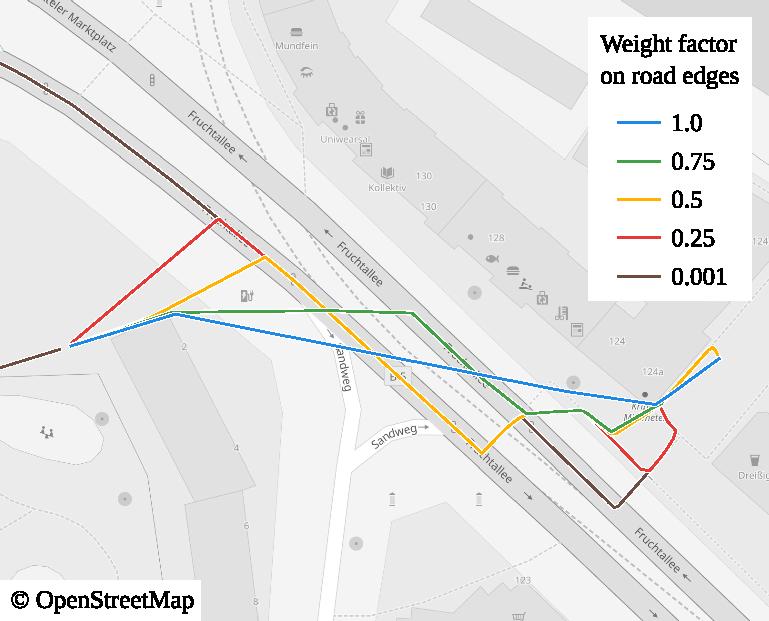
\includegraphics[width=0.65\textwidth]{images/qgis-routing-city-weights.pdf}
			\end{figcenter}
			\caption{Different preferences on edges. High factor prefers visibility edges, low factor prefers road edges.}
		\end{figure}
	\end{frame}
	
	\begin{frame}{Graph generation task performance}
		\begin{table}
			\begin{tabularx}{\textwidth}{p{2.925cm}>{\raggedleft\arraybackslash}p{2.075cm}R>{\raggedleft\arraybackslash}p{2.2cm}}
\toprule
\textbf{Operation}	& \textbf{Normal}	& \textbf{No roads}	& \textbf{No obstacles}	\\
\midrule
kNN search			&  5,957.97 ms		& 5,924.27 ms		&  0.01 ms				\\
Create graph		&    191.68 ms		&   210.40 ms		&  0.01 ms				\\
Get obstacles		&     42.53 ms		&    40.76 ms		&  0.78 ms				\\
Merge road edges	&  6,599.78 ms		&     5.67 ms		& 32.79 ms				\\
Add POI attributes	&      4.83 ms		&     1.53 ms		&  0.42 ms				\\
\midrule
Total time			& 12,853.51 ms		& 6,201.96 ms		& 37.19 ms				\\
\bottomrule
			\end{tabularx}
			\caption{Time of graph generation tasks on different variants of the 4 km\textsuperscript{2} \enquote{OSM city} dataset.}
		\end{table}
	\end{frame}
	
	\begin{frame}{Route quality analysis -- Examples (OSM city)}
		\begin{figure}
			\begin{figcenter}
				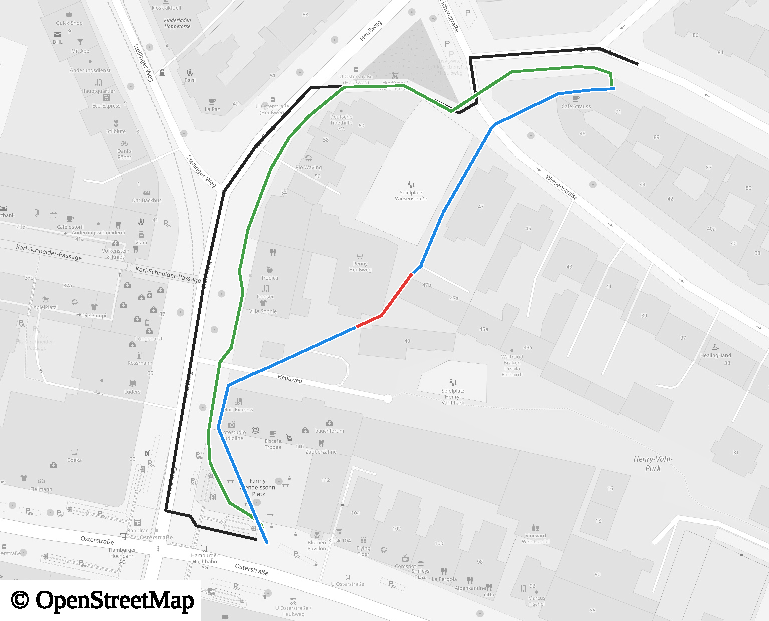
\includegraphics[width=0.65\textwidth]{../thesis/images/qgis-routing-city-routing-3.pdf}
			\end{figcenter}
			\caption{Expected (green), graph-based (black) and actual (blue) routes. Faulty passages marked in red.}
		\end{figure}
	\end{frame}
	
	\begin{frame}{Route quality analysis -- Examples (OSM rural)}
		\begin{figure}
			\begin{figcenter}
				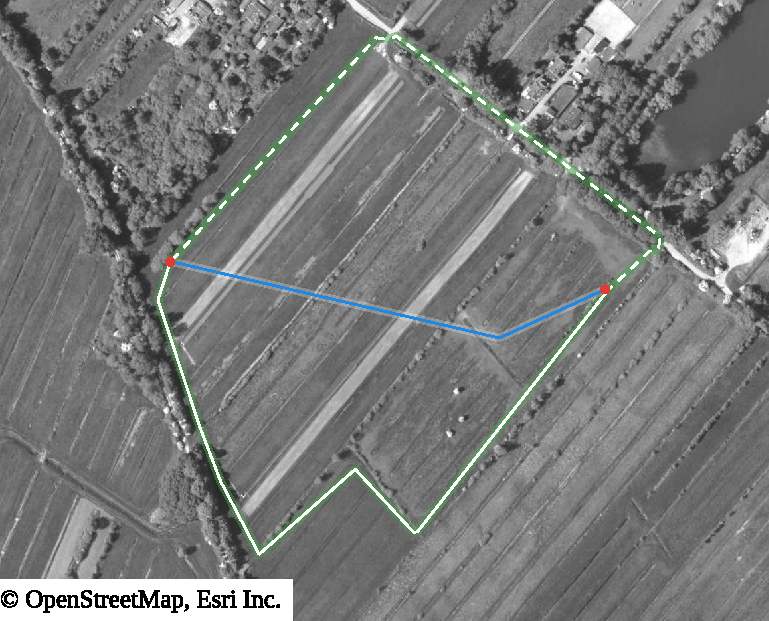
\includegraphics[width=0.65\textwidth]{../thesis/images/qgis-routing-rural-routing-6-aerial.pdf}
			\end{figcenter}
			\caption{Comparison of routes to aerial imagery.}
		\end{figure}
	\end{frame}
	
	\begin{frame}{Route quality analysis -- Examples (OSM rural)}
		\begin{figure}
			\begin{figcenter}
				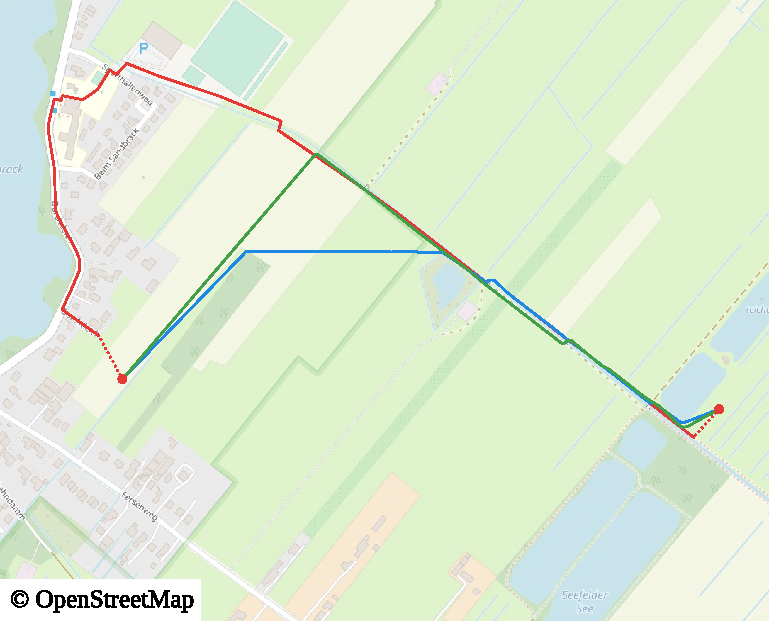
\includegraphics[width=0.65\textwidth]{../thesis/images/qgis-routing-rural-routing-17-graph-based.pdf}
			\end{figcenter}
			\caption{Expected (green), graph-based (red) and actual (blue) routes.}
		\end{figure}
	\end{frame}
	
	\begin{frame}{Routing performance}
		\begin{figure}
			\begin{figcenter}
				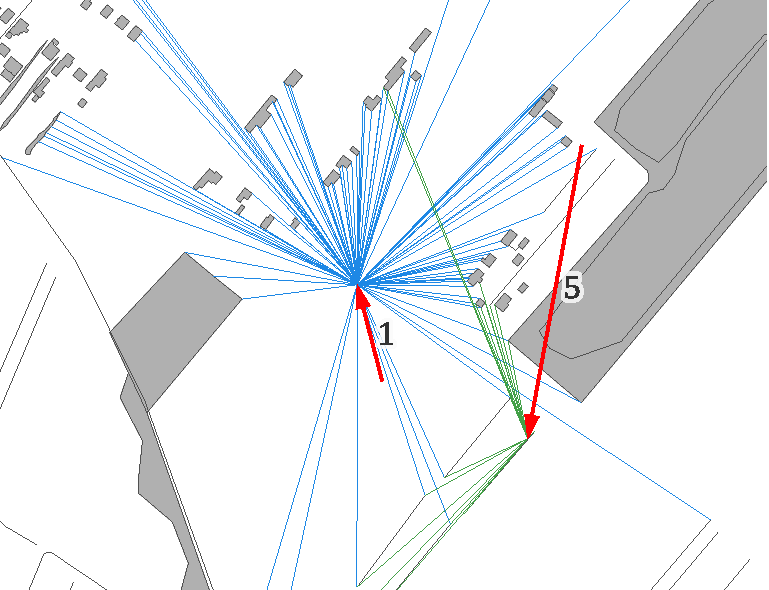
\includegraphics[width=0.65\textwidth]{../thesis/images/qgis-osm-rural.pdf}
			\end{figcenter}
			\caption{Edges creates for two routing requests in the \enquote{OSM rural} dataset.}
		\end{figure}
	\end{frame}
	
	\begin{frame}{Graph generation task performance}
		\begin{figure}
			\begin{figcenter}
				\hspace*{-0.35cm}
				\scalebox{0.7}
				{
					\begingroup%
\makeatletter%
\begin{pgfpicture}%
\pgfpathrectangle{\pgfpointorigin}{\pgfqpoint{6.035668in}{2.407638in}}%
\pgfusepath{use as bounding box}%
\begin{pgfscope}%
\pgfsetbuttcap%
\pgfsetmiterjoin%
\definecolor{currentfill}{rgb}{1.000000,1.000000,1.000000}%
\pgfsetfillcolor{currentfill}%
\pgfsetlinewidth{0.000000pt}%
\definecolor{currentstroke}{rgb}{1.000000,1.000000,1.000000}%
\pgfsetstrokecolor{currentstroke}%
\pgfsetdash{}{0pt}%
\pgfpathmoveto{\pgfqpoint{0.000000in}{0.000000in}}%
\pgfpathlineto{\pgfqpoint{6.035668in}{0.000000in}}%
\pgfpathlineto{\pgfqpoint{6.035668in}{2.407638in}}%
\pgfpathlineto{\pgfqpoint{0.000000in}{2.407638in}}%
\pgfpathlineto{\pgfqpoint{0.000000in}{0.000000in}}%
\pgfpathclose%
\pgfusepath{fill}%
\end{pgfscope}%
\begin{pgfscope}%
\pgfsetbuttcap%
\pgfsetmiterjoin%
\definecolor{currentfill}{rgb}{1.000000,1.000000,1.000000}%
\pgfsetfillcolor{currentfill}%
\pgfsetlinewidth{0.000000pt}%
\definecolor{currentstroke}{rgb}{0.000000,0.000000,0.000000}%
\pgfsetstrokecolor{currentstroke}%
\pgfsetstrokeopacity{0.000000}%
\pgfsetdash{}{0pt}%
\pgfpathmoveto{\pgfqpoint{0.497592in}{0.451389in}}%
\pgfpathlineto{\pgfqpoint{4.625417in}{0.451389in}}%
\pgfpathlineto{\pgfqpoint{4.625417in}{2.407638in}}%
\pgfpathlineto{\pgfqpoint{0.497592in}{2.407638in}}%
\pgfpathlineto{\pgfqpoint{0.497592in}{0.451389in}}%
\pgfpathclose%
\pgfusepath{fill}%
\end{pgfscope}%
\begin{pgfscope}%
\pgfpathrectangle{\pgfqpoint{0.497592in}{0.451389in}}{\pgfqpoint{4.127824in}{1.956249in}}%
\pgfusepath{clip}%
\pgfsetroundcap%
\pgfsetroundjoin%
\pgfsetlinewidth{1.003750pt}%
\definecolor{currentstroke}{rgb}{0.800000,0.800000,0.800000}%
\pgfsetstrokecolor{currentstroke}%
\pgfsetdash{}{0pt}%
\pgfpathmoveto{\pgfqpoint{0.497592in}{0.451389in}}%
\pgfpathlineto{\pgfqpoint{0.497592in}{2.407638in}}%
\pgfusepath{stroke}%
\end{pgfscope}%
\begin{pgfscope}%
\definecolor{textcolor}{rgb}{0.150000,0.150000,0.150000}%
\pgfsetstrokecolor{textcolor}%
\pgfsetfillcolor{textcolor}%
\pgftext[x=0.497592in,y=0.319444in,,top]{\color{textcolor}\sffamily\fontsize{9.000000}{10.800000}\selectfont 0}%
\end{pgfscope}%
\begin{pgfscope}%
\pgfpathrectangle{\pgfqpoint{0.497592in}{0.451389in}}{\pgfqpoint{4.127824in}{1.956249in}}%
\pgfusepath{clip}%
\pgfsetroundcap%
\pgfsetroundjoin%
\pgfsetlinewidth{1.003750pt}%
\definecolor{currentstroke}{rgb}{0.800000,0.800000,0.800000}%
\pgfsetstrokecolor{currentstroke}%
\pgfsetdash{}{0pt}%
\pgfpathmoveto{\pgfqpoint{1.377461in}{0.451389in}}%
\pgfpathlineto{\pgfqpoint{1.377461in}{2.407638in}}%
\pgfusepath{stroke}%
\end{pgfscope}%
\begin{pgfscope}%
\definecolor{textcolor}{rgb}{0.150000,0.150000,0.150000}%
\pgfsetstrokecolor{textcolor}%
\pgfsetfillcolor{textcolor}%
\pgftext[x=1.377461in,y=0.319444in,,top]{\color{textcolor}\sffamily\fontsize{9.000000}{10.800000}\selectfont 10000}%
\end{pgfscope}%
\begin{pgfscope}%
\pgfpathrectangle{\pgfqpoint{0.497592in}{0.451389in}}{\pgfqpoint{4.127824in}{1.956249in}}%
\pgfusepath{clip}%
\pgfsetroundcap%
\pgfsetroundjoin%
\pgfsetlinewidth{1.003750pt}%
\definecolor{currentstroke}{rgb}{0.800000,0.800000,0.800000}%
\pgfsetstrokecolor{currentstroke}%
\pgfsetdash{}{0pt}%
\pgfpathmoveto{\pgfqpoint{2.257329in}{0.451389in}}%
\pgfpathlineto{\pgfqpoint{2.257329in}{2.407638in}}%
\pgfusepath{stroke}%
\end{pgfscope}%
\begin{pgfscope}%
\definecolor{textcolor}{rgb}{0.150000,0.150000,0.150000}%
\pgfsetstrokecolor{textcolor}%
\pgfsetfillcolor{textcolor}%
\pgftext[x=2.257329in,y=0.319444in,,top]{\color{textcolor}\sffamily\fontsize{9.000000}{10.800000}\selectfont 20000}%
\end{pgfscope}%
\begin{pgfscope}%
\pgfpathrectangle{\pgfqpoint{0.497592in}{0.451389in}}{\pgfqpoint{4.127824in}{1.956249in}}%
\pgfusepath{clip}%
\pgfsetroundcap%
\pgfsetroundjoin%
\pgfsetlinewidth{1.003750pt}%
\definecolor{currentstroke}{rgb}{0.800000,0.800000,0.800000}%
\pgfsetstrokecolor{currentstroke}%
\pgfsetdash{}{0pt}%
\pgfpathmoveto{\pgfqpoint{3.137198in}{0.451389in}}%
\pgfpathlineto{\pgfqpoint{3.137198in}{2.407638in}}%
\pgfusepath{stroke}%
\end{pgfscope}%
\begin{pgfscope}%
\definecolor{textcolor}{rgb}{0.150000,0.150000,0.150000}%
\pgfsetstrokecolor{textcolor}%
\pgfsetfillcolor{textcolor}%
\pgftext[x=3.137198in,y=0.319444in,,top]{\color{textcolor}\sffamily\fontsize{9.000000}{10.800000}\selectfont 30000}%
\end{pgfscope}%
\begin{pgfscope}%
\pgfpathrectangle{\pgfqpoint{0.497592in}{0.451389in}}{\pgfqpoint{4.127824in}{1.956249in}}%
\pgfusepath{clip}%
\pgfsetroundcap%
\pgfsetroundjoin%
\pgfsetlinewidth{1.003750pt}%
\definecolor{currentstroke}{rgb}{0.800000,0.800000,0.800000}%
\pgfsetstrokecolor{currentstroke}%
\pgfsetdash{}{0pt}%
\pgfpathmoveto{\pgfqpoint{4.017067in}{0.451389in}}%
\pgfpathlineto{\pgfqpoint{4.017067in}{2.407638in}}%
\pgfusepath{stroke}%
\end{pgfscope}%
\begin{pgfscope}%
\definecolor{textcolor}{rgb}{0.150000,0.150000,0.150000}%
\pgfsetstrokecolor{textcolor}%
\pgfsetfillcolor{textcolor}%
\pgftext[x=4.017067in,y=0.319444in,,top]{\color{textcolor}\sffamily\fontsize{9.000000}{10.800000}\selectfont 40000}%
\end{pgfscope}%
\begin{pgfscope}%
\definecolor{textcolor}{rgb}{0.150000,0.150000,0.150000}%
\pgfsetstrokecolor{textcolor}%
\pgfsetfillcolor{textcolor}%
\pgftext[x=2.561504in,y=0.125000in,,top]{\color{textcolor}\sffamily\fontsize{9.000000}{10.800000}\selectfont Input obstacle vertices}%
\end{pgfscope}%
\begin{pgfscope}%
\pgfpathrectangle{\pgfqpoint{0.497592in}{0.451389in}}{\pgfqpoint{4.127824in}{1.956249in}}%
\pgfusepath{clip}%
\pgfsetroundcap%
\pgfsetroundjoin%
\pgfsetlinewidth{1.003750pt}%
\definecolor{currentstroke}{rgb}{0.800000,0.800000,0.800000}%
\pgfsetstrokecolor{currentstroke}%
\pgfsetdash{}{0pt}%
\pgfpathmoveto{\pgfqpoint{0.497592in}{0.451389in}}%
\pgfpathlineto{\pgfqpoint{4.625417in}{0.451389in}}%
\pgfusepath{stroke}%
\end{pgfscope}%
\begin{pgfscope}%
\definecolor{textcolor}{rgb}{0.150000,0.150000,0.150000}%
\pgfsetstrokecolor{textcolor}%
\pgfsetfillcolor{textcolor}%
\pgftext[x=0.194444in, y=0.403903in, left, base]{\color{textcolor}\sffamily\fontsize{9.000000}{10.800000}\selectfont 0.0}%
\end{pgfscope}%
\begin{pgfscope}%
\pgfpathrectangle{\pgfqpoint{0.497592in}{0.451389in}}{\pgfqpoint{4.127824in}{1.956249in}}%
\pgfusepath{clip}%
\pgfsetroundcap%
\pgfsetroundjoin%
\pgfsetlinewidth{1.003750pt}%
\definecolor{currentstroke}{rgb}{0.800000,0.800000,0.800000}%
\pgfsetstrokecolor{currentstroke}%
\pgfsetdash{}{0pt}%
\pgfpathmoveto{\pgfqpoint{0.497592in}{0.824009in}}%
\pgfpathlineto{\pgfqpoint{4.625417in}{0.824009in}}%
\pgfusepath{stroke}%
\end{pgfscope}%
\begin{pgfscope}%
\definecolor{textcolor}{rgb}{0.150000,0.150000,0.150000}%
\pgfsetstrokecolor{textcolor}%
\pgfsetfillcolor{textcolor}%
\pgftext[x=0.194444in, y=0.776524in, left, base]{\color{textcolor}\sffamily\fontsize{9.000000}{10.800000}\selectfont 0.2}%
\end{pgfscope}%
\begin{pgfscope}%
\pgfpathrectangle{\pgfqpoint{0.497592in}{0.451389in}}{\pgfqpoint{4.127824in}{1.956249in}}%
\pgfusepath{clip}%
\pgfsetroundcap%
\pgfsetroundjoin%
\pgfsetlinewidth{1.003750pt}%
\definecolor{currentstroke}{rgb}{0.800000,0.800000,0.800000}%
\pgfsetstrokecolor{currentstroke}%
\pgfsetdash{}{0pt}%
\pgfpathmoveto{\pgfqpoint{0.497592in}{1.196629in}}%
\pgfpathlineto{\pgfqpoint{4.625417in}{1.196629in}}%
\pgfusepath{stroke}%
\end{pgfscope}%
\begin{pgfscope}%
\definecolor{textcolor}{rgb}{0.150000,0.150000,0.150000}%
\pgfsetstrokecolor{textcolor}%
\pgfsetfillcolor{textcolor}%
\pgftext[x=0.194444in, y=1.149144in, left, base]{\color{textcolor}\sffamily\fontsize{9.000000}{10.800000}\selectfont 0.4}%
\end{pgfscope}%
\begin{pgfscope}%
\pgfpathrectangle{\pgfqpoint{0.497592in}{0.451389in}}{\pgfqpoint{4.127824in}{1.956249in}}%
\pgfusepath{clip}%
\pgfsetroundcap%
\pgfsetroundjoin%
\pgfsetlinewidth{1.003750pt}%
\definecolor{currentstroke}{rgb}{0.800000,0.800000,0.800000}%
\pgfsetstrokecolor{currentstroke}%
\pgfsetdash{}{0pt}%
\pgfpathmoveto{\pgfqpoint{0.497592in}{1.569250in}}%
\pgfpathlineto{\pgfqpoint{4.625417in}{1.569250in}}%
\pgfusepath{stroke}%
\end{pgfscope}%
\begin{pgfscope}%
\definecolor{textcolor}{rgb}{0.150000,0.150000,0.150000}%
\pgfsetstrokecolor{textcolor}%
\pgfsetfillcolor{textcolor}%
\pgftext[x=0.194444in, y=1.521764in, left, base]{\color{textcolor}\sffamily\fontsize{9.000000}{10.800000}\selectfont 0.6}%
\end{pgfscope}%
\begin{pgfscope}%
\pgfpathrectangle{\pgfqpoint{0.497592in}{0.451389in}}{\pgfqpoint{4.127824in}{1.956249in}}%
\pgfusepath{clip}%
\pgfsetroundcap%
\pgfsetroundjoin%
\pgfsetlinewidth{1.003750pt}%
\definecolor{currentstroke}{rgb}{0.800000,0.800000,0.800000}%
\pgfsetstrokecolor{currentstroke}%
\pgfsetdash{}{0pt}%
\pgfpathmoveto{\pgfqpoint{0.497592in}{1.941870in}}%
\pgfpathlineto{\pgfqpoint{4.625417in}{1.941870in}}%
\pgfusepath{stroke}%
\end{pgfscope}%
\begin{pgfscope}%
\definecolor{textcolor}{rgb}{0.150000,0.150000,0.150000}%
\pgfsetstrokecolor{textcolor}%
\pgfsetfillcolor{textcolor}%
\pgftext[x=0.194444in, y=1.894385in, left, base]{\color{textcolor}\sffamily\fontsize{9.000000}{10.800000}\selectfont 0.8}%
\end{pgfscope}%
\begin{pgfscope}%
\pgfpathrectangle{\pgfqpoint{0.497592in}{0.451389in}}{\pgfqpoint{4.127824in}{1.956249in}}%
\pgfusepath{clip}%
\pgfsetroundcap%
\pgfsetroundjoin%
\pgfsetlinewidth{1.003750pt}%
\definecolor{currentstroke}{rgb}{0.800000,0.800000,0.800000}%
\pgfsetstrokecolor{currentstroke}%
\pgfsetdash{}{0pt}%
\pgfpathmoveto{\pgfqpoint{0.497592in}{2.314490in}}%
\pgfpathlineto{\pgfqpoint{4.625417in}{2.314490in}}%
\pgfusepath{stroke}%
\end{pgfscope}%
\begin{pgfscope}%
\definecolor{textcolor}{rgb}{0.150000,0.150000,0.150000}%
\pgfsetstrokecolor{textcolor}%
\pgfsetfillcolor{textcolor}%
\pgftext[x=0.194444in, y=2.267005in, left, base]{\color{textcolor}\sffamily\fontsize{9.000000}{10.800000}\selectfont 1.0}%
\end{pgfscope}%
\begin{pgfscope}%
\definecolor{textcolor}{rgb}{0.150000,0.150000,0.150000}%
\pgfsetstrokecolor{textcolor}%
\pgfsetfillcolor{textcolor}%
\pgftext[x=0.125000in,y=1.429513in,,bottom,rotate=90.000000]{\color{textcolor}\sffamily\fontsize{9.000000}{10.800000}\selectfont Share of total time}%
\end{pgfscope}%
\begin{pgfscope}%
\pgfpathrectangle{\pgfqpoint{0.497592in}{0.451389in}}{\pgfqpoint{4.127824in}{1.956249in}}%
\pgfusepath{clip}%
\pgfsetbuttcap%
\pgfsetroundjoin%
\definecolor{currentfill}{rgb}{0.003922,0.450980,0.698039}%
\pgfsetfillcolor{currentfill}%
\pgfsetfillopacity{0.200000}%
\pgfsetlinewidth{1.003750pt}%
\definecolor{currentstroke}{rgb}{0.003922,0.450980,0.698039}%
\pgfsetstrokecolor{currentstroke}%
\pgfsetstrokeopacity{0.200000}%
\pgfsetdash{}{0pt}%
\pgfsys@defobject{currentmarker}{\pgfqpoint{1.121947in}{2.314490in}}{\pgfqpoint{4.458585in}{2.314490in}}{%
\pgfpathmoveto{\pgfqpoint{1.121947in}{2.314490in}}%
\pgfpathlineto{\pgfqpoint{1.121947in}{2.314490in}}%
\pgfpathlineto{\pgfqpoint{1.628927in}{2.314490in}}%
\pgfpathlineto{\pgfqpoint{2.072029in}{2.314490in}}%
\pgfpathlineto{\pgfqpoint{2.503781in}{2.314490in}}%
\pgfpathlineto{\pgfqpoint{3.507975in}{2.314490in}}%
\pgfpathlineto{\pgfqpoint{4.458585in}{2.314490in}}%
\pgfpathlineto{\pgfqpoint{4.458585in}{2.314490in}}%
\pgfpathlineto{\pgfqpoint{4.458585in}{2.314490in}}%
\pgfpathlineto{\pgfqpoint{3.507975in}{2.314490in}}%
\pgfpathlineto{\pgfqpoint{2.503781in}{2.314490in}}%
\pgfpathlineto{\pgfqpoint{2.072029in}{2.314490in}}%
\pgfpathlineto{\pgfqpoint{1.628927in}{2.314490in}}%
\pgfpathlineto{\pgfqpoint{1.121947in}{2.314490in}}%
\pgfpathlineto{\pgfqpoint{1.121947in}{2.314490in}}%
\pgfpathclose%
\pgfusepath{stroke,fill}%
}%
\begin{pgfscope}%
\pgfsys@transformshift{0.000000in}{0.000000in}%
\pgfsys@useobject{currentmarker}{}%
\end{pgfscope}%
\end{pgfscope}%
\begin{pgfscope}%
\pgfpathrectangle{\pgfqpoint{0.497592in}{0.451389in}}{\pgfqpoint{4.127824in}{1.956249in}}%
\pgfusepath{clip}%
\pgfsetbuttcap%
\pgfsetroundjoin%
\definecolor{currentfill}{rgb}{0.870588,0.560784,0.019608}%
\pgfsetfillcolor{currentfill}%
\pgfsetfillopacity{0.200000}%
\pgfsetlinewidth{1.003750pt}%
\definecolor{currentstroke}{rgb}{0.870588,0.560784,0.019608}%
\pgfsetstrokecolor{currentstroke}%
\pgfsetstrokeopacity{0.200000}%
\pgfsetdash{}{0pt}%
\pgfsys@defobject{currentmarker}{\pgfqpoint{1.121947in}{1.604424in}}{\pgfqpoint{4.458585in}{1.805244in}}{%
\pgfpathmoveto{\pgfqpoint{1.121947in}{1.654451in}}%
\pgfpathlineto{\pgfqpoint{1.121947in}{1.621510in}}%
\pgfpathlineto{\pgfqpoint{1.628927in}{1.633094in}}%
\pgfpathlineto{\pgfqpoint{2.072029in}{1.604424in}}%
\pgfpathlineto{\pgfqpoint{2.503781in}{1.607552in}}%
\pgfpathlineto{\pgfqpoint{3.507975in}{1.692166in}}%
\pgfpathlineto{\pgfqpoint{4.458585in}{1.786127in}}%
\pgfpathlineto{\pgfqpoint{4.458585in}{1.805244in}}%
\pgfpathlineto{\pgfqpoint{4.458585in}{1.805244in}}%
\pgfpathlineto{\pgfqpoint{3.507975in}{1.703495in}}%
\pgfpathlineto{\pgfqpoint{2.503781in}{1.624051in}}%
\pgfpathlineto{\pgfqpoint{2.072029in}{1.623827in}}%
\pgfpathlineto{\pgfqpoint{1.628927in}{1.639324in}}%
\pgfpathlineto{\pgfqpoint{1.121947in}{1.654451in}}%
\pgfpathlineto{\pgfqpoint{1.121947in}{1.654451in}}%
\pgfpathclose%
\pgfusepath{stroke,fill}%
}%
\begin{pgfscope}%
\pgfsys@transformshift{0.000000in}{0.000000in}%
\pgfsys@useobject{currentmarker}{}%
\end{pgfscope}%
\end{pgfscope}%
\begin{pgfscope}%
\pgfpathrectangle{\pgfqpoint{0.497592in}{0.451389in}}{\pgfqpoint{4.127824in}{1.956249in}}%
\pgfusepath{clip}%
\pgfsetbuttcap%
\pgfsetroundjoin%
\definecolor{currentfill}{rgb}{0.007843,0.619608,0.450980}%
\pgfsetfillcolor{currentfill}%
\pgfsetfillopacity{0.200000}%
\pgfsetlinewidth{1.003750pt}%
\definecolor{currentstroke}{rgb}{0.007843,0.619608,0.450980}%
\pgfsetstrokecolor{currentstroke}%
\pgfsetstrokeopacity{0.200000}%
\pgfsetdash{}{0pt}%
\pgfsys@defobject{currentmarker}{\pgfqpoint{1.121947in}{0.454227in}}{\pgfqpoint{4.458585in}{0.468429in}}{%
\pgfpathmoveto{\pgfqpoint{1.121947in}{0.468429in}}%
\pgfpathlineto{\pgfqpoint{1.121947in}{0.466842in}}%
\pgfpathlineto{\pgfqpoint{1.628927in}{0.462249in}}%
\pgfpathlineto{\pgfqpoint{2.072029in}{0.459512in}}%
\pgfpathlineto{\pgfqpoint{2.503781in}{0.457824in}}%
\pgfpathlineto{\pgfqpoint{3.507975in}{0.455694in}}%
\pgfpathlineto{\pgfqpoint{4.458585in}{0.454227in}}%
\pgfpathlineto{\pgfqpoint{4.458585in}{0.454424in}}%
\pgfpathlineto{\pgfqpoint{4.458585in}{0.454424in}}%
\pgfpathlineto{\pgfqpoint{3.507975in}{0.455824in}}%
\pgfpathlineto{\pgfqpoint{2.503781in}{0.461259in}}%
\pgfpathlineto{\pgfqpoint{2.072029in}{0.459760in}}%
\pgfpathlineto{\pgfqpoint{1.628927in}{0.462461in}}%
\pgfpathlineto{\pgfqpoint{1.121947in}{0.468429in}}%
\pgfpathlineto{\pgfqpoint{1.121947in}{0.468429in}}%
\pgfpathclose%
\pgfusepath{stroke,fill}%
}%
\begin{pgfscope}%
\pgfsys@transformshift{0.000000in}{0.000000in}%
\pgfsys@useobject{currentmarker}{}%
\end{pgfscope}%
\end{pgfscope}%
\begin{pgfscope}%
\pgfpathrectangle{\pgfqpoint{0.497592in}{0.451389in}}{\pgfqpoint{4.127824in}{1.956249in}}%
\pgfusepath{clip}%
\pgfsetbuttcap%
\pgfsetroundjoin%
\definecolor{currentfill}{rgb}{0.835294,0.368627,0.000000}%
\pgfsetfillcolor{currentfill}%
\pgfsetfillopacity{0.200000}%
\pgfsetlinewidth{1.003750pt}%
\definecolor{currentstroke}{rgb}{0.835294,0.368627,0.000000}%
\pgfsetstrokecolor{currentstroke}%
\pgfsetstrokeopacity{0.200000}%
\pgfsetdash{}{0pt}%
\pgfsys@defobject{currentmarker}{\pgfqpoint{1.121947in}{0.452609in}}{\pgfqpoint{4.458585in}{0.464052in}}{%
\pgfpathmoveto{\pgfqpoint{1.121947in}{0.464052in}}%
\pgfpathlineto{\pgfqpoint{1.121947in}{0.459896in}}%
\pgfpathlineto{\pgfqpoint{1.628927in}{0.456498in}}%
\pgfpathlineto{\pgfqpoint{2.072029in}{0.455315in}}%
\pgfpathlineto{\pgfqpoint{2.503781in}{0.454348in}}%
\pgfpathlineto{\pgfqpoint{3.507975in}{0.453264in}}%
\pgfpathlineto{\pgfqpoint{4.458585in}{0.452609in}}%
\pgfpathlineto{\pgfqpoint{4.458585in}{0.452750in}}%
\pgfpathlineto{\pgfqpoint{4.458585in}{0.452750in}}%
\pgfpathlineto{\pgfqpoint{3.507975in}{0.453418in}}%
\pgfpathlineto{\pgfqpoint{2.503781in}{0.454588in}}%
\pgfpathlineto{\pgfqpoint{2.072029in}{0.455746in}}%
\pgfpathlineto{\pgfqpoint{1.628927in}{0.457501in}}%
\pgfpathlineto{\pgfqpoint{1.121947in}{0.464052in}}%
\pgfpathlineto{\pgfqpoint{1.121947in}{0.464052in}}%
\pgfpathclose%
\pgfusepath{stroke,fill}%
}%
\begin{pgfscope}%
\pgfsys@transformshift{0.000000in}{0.000000in}%
\pgfsys@useobject{currentmarker}{}%
\end{pgfscope}%
\end{pgfscope}%
\begin{pgfscope}%
\pgfpathrectangle{\pgfqpoint{0.497592in}{0.451389in}}{\pgfqpoint{4.127824in}{1.956249in}}%
\pgfusepath{clip}%
\pgfsetbuttcap%
\pgfsetroundjoin%
\definecolor{currentfill}{rgb}{0.800000,0.470588,0.737255}%
\pgfsetfillcolor{currentfill}%
\pgfsetfillopacity{0.200000}%
\pgfsetlinewidth{1.003750pt}%
\definecolor{currentstroke}{rgb}{0.800000,0.470588,0.737255}%
\pgfsetstrokecolor{currentstroke}%
\pgfsetstrokeopacity{0.200000}%
\pgfsetdash{}{0pt}%
\pgfsys@defobject{currentmarker}{\pgfqpoint{1.121947in}{0.954945in}}{\pgfqpoint{4.458585in}{1.144078in}}{%
\pgfpathmoveto{\pgfqpoint{1.121947in}{1.107867in}}%
\pgfpathlineto{\pgfqpoint{1.121947in}{1.077066in}}%
\pgfpathlineto{\pgfqpoint{1.628927in}{1.104104in}}%
\pgfpathlineto{\pgfqpoint{2.072029in}{1.124854in}}%
\pgfpathlineto{\pgfqpoint{2.503781in}{1.127704in}}%
\pgfpathlineto{\pgfqpoint{3.507975in}{1.053898in}}%
\pgfpathlineto{\pgfqpoint{4.458585in}{0.954945in}}%
\pgfpathlineto{\pgfqpoint{4.458585in}{0.973668in}}%
\pgfpathlineto{\pgfqpoint{4.458585in}{0.973668in}}%
\pgfpathlineto{\pgfqpoint{3.507975in}{1.065148in}}%
\pgfpathlineto{\pgfqpoint{2.503781in}{1.142337in}}%
\pgfpathlineto{\pgfqpoint{2.072029in}{1.144078in}}%
\pgfpathlineto{\pgfqpoint{1.628927in}{1.110633in}}%
\pgfpathlineto{\pgfqpoint{1.121947in}{1.107867in}}%
\pgfpathlineto{\pgfqpoint{1.121947in}{1.107867in}}%
\pgfpathclose%
\pgfusepath{stroke,fill}%
}%
\begin{pgfscope}%
\pgfsys@transformshift{0.000000in}{0.000000in}%
\pgfsys@useobject{currentmarker}{}%
\end{pgfscope}%
\end{pgfscope}%
\begin{pgfscope}%
\pgfpathrectangle{\pgfqpoint{0.497592in}{0.451389in}}{\pgfqpoint{4.127824in}{1.956249in}}%
\pgfusepath{clip}%
\pgfsetbuttcap%
\pgfsetroundjoin%
\definecolor{currentfill}{rgb}{0.792157,0.568627,0.380392}%
\pgfsetfillcolor{currentfill}%
\pgfsetfillopacity{0.200000}%
\pgfsetlinewidth{1.003750pt}%
\definecolor{currentstroke}{rgb}{0.792157,0.568627,0.380392}%
\pgfsetstrokecolor{currentstroke}%
\pgfsetstrokeopacity{0.200000}%
\pgfsetdash{}{0pt}%
\pgfsys@defobject{currentmarker}{\pgfqpoint{1.121947in}{0.451545in}}{\pgfqpoint{4.458585in}{0.452461in}}{%
\pgfpathmoveto{\pgfqpoint{1.121947in}{0.452461in}}%
\pgfpathlineto{\pgfqpoint{1.121947in}{0.452336in}}%
\pgfpathlineto{\pgfqpoint{1.628927in}{0.452066in}}%
\pgfpathlineto{\pgfqpoint{2.072029in}{0.451992in}}%
\pgfpathlineto{\pgfqpoint{2.503781in}{0.451814in}}%
\pgfpathlineto{\pgfqpoint{3.507975in}{0.451620in}}%
\pgfpathlineto{\pgfqpoint{4.458585in}{0.451545in}}%
\pgfpathlineto{\pgfqpoint{4.458585in}{0.451655in}}%
\pgfpathlineto{\pgfqpoint{4.458585in}{0.451655in}}%
\pgfpathlineto{\pgfqpoint{3.507975in}{0.451632in}}%
\pgfpathlineto{\pgfqpoint{2.503781in}{0.451879in}}%
\pgfpathlineto{\pgfqpoint{2.072029in}{0.452091in}}%
\pgfpathlineto{\pgfqpoint{1.628927in}{0.452292in}}%
\pgfpathlineto{\pgfqpoint{1.121947in}{0.452461in}}%
\pgfpathlineto{\pgfqpoint{1.121947in}{0.452461in}}%
\pgfpathclose%
\pgfusepath{stroke,fill}%
}%
\begin{pgfscope}%
\pgfsys@transformshift{0.000000in}{0.000000in}%
\pgfsys@useobject{currentmarker}{}%
\end{pgfscope}%
\end{pgfscope}%
\begin{pgfscope}%
\pgfsetrectcap%
\pgfsetmiterjoin%
\pgfsetlinewidth{1.254687pt}%
\definecolor{currentstroke}{rgb}{0.800000,0.800000,0.800000}%
\pgfsetstrokecolor{currentstroke}%
\pgfsetdash{}{0pt}%
\pgfpathmoveto{\pgfqpoint{0.497592in}{0.451389in}}%
\pgfpathlineto{\pgfqpoint{0.497592in}{2.407638in}}%
\pgfusepath{stroke}%
\end{pgfscope}%
\begin{pgfscope}%
\pgfsetrectcap%
\pgfsetmiterjoin%
\pgfsetlinewidth{1.254687pt}%
\definecolor{currentstroke}{rgb}{0.800000,0.800000,0.800000}%
\pgfsetstrokecolor{currentstroke}%
\pgfsetdash{}{0pt}%
\pgfpathmoveto{\pgfqpoint{4.625417in}{0.451389in}}%
\pgfpathlineto{\pgfqpoint{4.625417in}{2.407638in}}%
\pgfusepath{stroke}%
\end{pgfscope}%
\begin{pgfscope}%
\pgfsetrectcap%
\pgfsetmiterjoin%
\pgfsetlinewidth{1.254687pt}%
\definecolor{currentstroke}{rgb}{0.800000,0.800000,0.800000}%
\pgfsetstrokecolor{currentstroke}%
\pgfsetdash{}{0pt}%
\pgfpathmoveto{\pgfqpoint{0.497592in}{0.451389in}}%
\pgfpathlineto{\pgfqpoint{4.625417in}{0.451389in}}%
\pgfusepath{stroke}%
\end{pgfscope}%
\begin{pgfscope}%
\pgfsetrectcap%
\pgfsetmiterjoin%
\pgfsetlinewidth{1.254687pt}%
\definecolor{currentstroke}{rgb}{0.800000,0.800000,0.800000}%
\pgfsetstrokecolor{currentstroke}%
\pgfsetdash{}{0pt}%
\pgfpathmoveto{\pgfqpoint{0.497592in}{2.407638in}}%
\pgfpathlineto{\pgfqpoint{4.625417in}{2.407638in}}%
\pgfusepath{stroke}%
\end{pgfscope}%
\begin{pgfscope}%
\pgfsetbuttcap%
\pgfsetmiterjoin%
\definecolor{currentfill}{rgb}{1.000000,1.000000,1.000000}%
\pgfsetfillcolor{currentfill}%
\pgfsetfillopacity{0.800000}%
\pgfsetlinewidth{1.003750pt}%
\definecolor{currentstroke}{rgb}{0.800000,0.800000,0.800000}%
\pgfsetstrokecolor{currentstroke}%
\pgfsetstrokeopacity{0.800000}%
\pgfsetdash{}{0pt}%
\pgfpathmoveto{\pgfqpoint{4.816112in}{0.538523in}}%
\pgfpathlineto{\pgfqpoint{6.010668in}{0.538523in}}%
\pgfpathquadraticcurveto{\pgfqpoint{6.035668in}{0.538523in}}{\pgfqpoint{6.035668in}{0.563523in}}%
\pgfpathlineto{\pgfqpoint{6.035668in}{2.295504in}}%
\pgfpathquadraticcurveto{\pgfqpoint{6.035668in}{2.320504in}}{\pgfqpoint{6.010668in}{2.320504in}}%
\pgfpathlineto{\pgfqpoint{4.816112in}{2.320504in}}%
\pgfpathquadraticcurveto{\pgfqpoint{4.791112in}{2.320504in}}{\pgfqpoint{4.791112in}{2.295504in}}%
\pgfpathlineto{\pgfqpoint{4.791112in}{0.563523in}}%
\pgfpathquadraticcurveto{\pgfqpoint{4.791112in}{0.538523in}}{\pgfqpoint{4.816112in}{0.538523in}}%
\pgfpathlineto{\pgfqpoint{4.816112in}{0.538523in}}%
\pgfpathclose%
\pgfusepath{stroke,fill}%
\end{pgfscope}%
\begin{pgfscope}%
\definecolor{textcolor}{rgb}{0.150000,0.150000,0.150000}%
\pgfsetstrokecolor{textcolor}%
\pgfsetfillcolor{textcolor}%
\pgftext[x=5.209990in,y=2.175533in,left,base]{\color{textcolor}\sffamily\fontsize{9.000000}{10.800000}\selectfont Legend}%
\end{pgfscope}%
\begin{pgfscope}%
\pgfsetroundcap%
\pgfsetroundjoin%
\pgfsetlinewidth{1.505625pt}%
\definecolor{currentstroke}{rgb}{0.003922,0.450980,0.698039}%
\pgfsetstrokecolor{currentstroke}%
\pgfsetdash{}{0pt}%
\pgfpathmoveto{\pgfqpoint{4.841112in}{2.031783in}}%
\pgfpathlineto{\pgfqpoint{4.966112in}{2.031783in}}%
\pgfpathlineto{\pgfqpoint{5.091112in}{2.031783in}}%
\pgfusepath{stroke}%
\end{pgfscope}%
\begin{pgfscope}%
\definecolor{textcolor}{rgb}{0.150000,0.150000,0.150000}%
\pgfsetstrokecolor{textcolor}%
\pgfsetfillcolor{textcolor}%
\pgftext[x=5.191112in,y=1.988033in,left,base]{\color{textcolor}\sffamily\fontsize{9.000000}{10.800000}\selectfont Total time}%
\end{pgfscope}%
\begin{pgfscope}%
\pgfsetroundcap%
\pgfsetroundjoin%
\pgfsetlinewidth{1.505625pt}%
\definecolor{currentstroke}{rgb}{0.870588,0.560784,0.019608}%
\pgfsetstrokecolor{currentstroke}%
\pgfsetdash{}{0pt}%
\pgfpathmoveto{\pgfqpoint{4.841112in}{1.844283in}}%
\pgfpathlineto{\pgfqpoint{4.966112in}{1.844283in}}%
\pgfpathlineto{\pgfqpoint{5.091112in}{1.844283in}}%
\pgfusepath{stroke}%
\end{pgfscope}%
\begin{pgfscope}%
\definecolor{textcolor}{rgb}{0.150000,0.150000,0.150000}%
\pgfsetstrokecolor{textcolor}%
\pgfsetfillcolor{textcolor}%
\pgftext[x=5.191112in,y=1.800533in,left,base]{\color{textcolor}\sffamily\fontsize{9.000000}{10.800000}\selectfont kNN search}%
\end{pgfscope}%
\begin{pgfscope}%
\pgfsetroundcap%
\pgfsetroundjoin%
\pgfsetlinewidth{1.505625pt}%
\definecolor{currentstroke}{rgb}{0.007843,0.619608,0.450980}%
\pgfsetstrokecolor{currentstroke}%
\pgfsetdash{}{0pt}%
\pgfpathmoveto{\pgfqpoint{4.841112in}{1.656783in}}%
\pgfpathlineto{\pgfqpoint{4.966112in}{1.656783in}}%
\pgfpathlineto{\pgfqpoint{5.091112in}{1.656783in}}%
\pgfusepath{stroke}%
\end{pgfscope}%
\begin{pgfscope}%
\definecolor{textcolor}{rgb}{0.150000,0.150000,0.150000}%
\pgfsetstrokecolor{textcolor}%
\pgfsetfillcolor{textcolor}%
\pgftext[x=5.191112in,y=1.613033in,left,base]{\color{textcolor}\sffamily\fontsize{9.000000}{10.800000}\selectfont Create graph}%
\end{pgfscope}%
\begin{pgfscope}%
\pgfsetroundcap%
\pgfsetroundjoin%
\pgfsetlinewidth{1.505625pt}%
\definecolor{currentstroke}{rgb}{0.835294,0.368627,0.000000}%
\pgfsetstrokecolor{currentstroke}%
\pgfsetdash{}{0pt}%
\pgfpathmoveto{\pgfqpoint{4.841112in}{1.382272in}}%
\pgfpathlineto{\pgfqpoint{4.966112in}{1.382272in}}%
\pgfpathlineto{\pgfqpoint{5.091112in}{1.382272in}}%
\pgfusepath{stroke}%
\end{pgfscope}%
\begin{pgfscope}%
\definecolor{textcolor}{rgb}{0.150000,0.150000,0.150000}%
\pgfsetstrokecolor{textcolor}%
\pgfsetfillcolor{textcolor}%
\pgftext[x=5.191112in, y=1.425534in, left, base]{\color{textcolor}\sffamily\fontsize{9.000000}{10.800000}\selectfont Get \& prepare}%
\end{pgfscope}%
\begin{pgfscope}%
\definecolor{textcolor}{rgb}{0.150000,0.150000,0.150000}%
\pgfsetstrokecolor{textcolor}%
\pgfsetfillcolor{textcolor}%
\pgftext[x=5.191112in, y=1.281540in, left, base]{\color{textcolor}\sffamily\fontsize{9.000000}{10.800000}\selectfont obstacles}%
\end{pgfscope}%
\begin{pgfscope}%
\pgfsetroundcap%
\pgfsetroundjoin%
\pgfsetlinewidth{1.505625pt}%
\definecolor{currentstroke}{rgb}{0.800000,0.470588,0.737255}%
\pgfsetstrokecolor{currentstroke}%
\pgfsetdash{}{0pt}%
\pgfpathmoveto{\pgfqpoint{4.841112in}{1.050778in}}%
\pgfpathlineto{\pgfqpoint{4.966112in}{1.050778in}}%
\pgfpathlineto{\pgfqpoint{5.091112in}{1.050778in}}%
\pgfusepath{stroke}%
\end{pgfscope}%
\begin{pgfscope}%
\definecolor{textcolor}{rgb}{0.150000,0.150000,0.150000}%
\pgfsetstrokecolor{textcolor}%
\pgfsetfillcolor{textcolor}%
\pgftext[x=5.191112in, y=1.094040in, left, base]{\color{textcolor}\sffamily\fontsize{9.000000}{10.800000}\selectfont Merge road}%
\end{pgfscope}%
\begin{pgfscope}%
\definecolor{textcolor}{rgb}{0.150000,0.150000,0.150000}%
\pgfsetstrokecolor{textcolor}%
\pgfsetfillcolor{textcolor}%
\pgftext[x=5.191112in, y=0.950046in, left, base]{\color{textcolor}\sffamily\fontsize{9.000000}{10.800000}\selectfont edges}%
\end{pgfscope}%
\begin{pgfscope}%
\pgfsetroundcap%
\pgfsetroundjoin%
\pgfsetlinewidth{1.505625pt}%
\definecolor{currentstroke}{rgb}{0.792157,0.568627,0.380392}%
\pgfsetstrokecolor{currentstroke}%
\pgfsetdash{}{0pt}%
\pgfpathmoveto{\pgfqpoint{4.841112in}{0.719284in}}%
\pgfpathlineto{\pgfqpoint{4.966112in}{0.719284in}}%
\pgfpathlineto{\pgfqpoint{5.091112in}{0.719284in}}%
\pgfusepath{stroke}%
\end{pgfscope}%
\begin{pgfscope}%
\definecolor{textcolor}{rgb}{0.150000,0.150000,0.150000}%
\pgfsetstrokecolor{textcolor}%
\pgfsetfillcolor{textcolor}%
\pgftext[x=5.191112in, y=0.762546in, left, base]{\color{textcolor}\sffamily\fontsize{9.000000}{10.800000}\selectfont Add POI}%
\end{pgfscope}%
\begin{pgfscope}%
\definecolor{textcolor}{rgb}{0.150000,0.150000,0.150000}%
\pgfsetstrokecolor{textcolor}%
\pgfsetfillcolor{textcolor}%
\pgftext[x=5.191112in, y=0.618552in, left, base]{\color{textcolor}\sffamily\fontsize{9.000000}{10.800000}\selectfont attributes}%
\end{pgfscope}%
\begin{pgfscope}%
\pgfsetroundcap%
\pgfsetroundjoin%
\pgfsetlinewidth{1.003750pt}%
\definecolor{currentstroke}{rgb}{0.003922,0.450980,0.698039}%
\pgfsetstrokecolor{currentstroke}%
\pgfsetdash{}{0pt}%
\pgfpathmoveto{\pgfqpoint{1.121947in}{2.314490in}}%
\pgfpathlineto{\pgfqpoint{1.628927in}{2.314490in}}%
\pgfpathlineto{\pgfqpoint{2.072029in}{2.314490in}}%
\pgfpathlineto{\pgfqpoint{2.503781in}{2.314490in}}%
\pgfpathlineto{\pgfqpoint{3.507975in}{2.314490in}}%
\pgfpathlineto{\pgfqpoint{4.458585in}{2.314490in}}%
\pgfusepath{stroke}%
\end{pgfscope}%
\begin{pgfscope}%
\pgfsetbuttcap%
\pgfsetroundjoin%
\definecolor{currentfill}{rgb}{0.003922,0.450980,0.698039}%
\pgfsetfillcolor{currentfill}%
\pgfsetlinewidth{0.752812pt}%
\definecolor{currentstroke}{rgb}{1.000000,1.000000,1.000000}%
\pgfsetstrokecolor{currentstroke}%
\pgfsetdash{}{0pt}%
\pgfsys@defobject{currentmarker}{\pgfqpoint{-0.034722in}{-0.034722in}}{\pgfqpoint{0.034722in}{0.034722in}}{%
\pgfpathmoveto{\pgfqpoint{0.000000in}{-0.034722in}}%
\pgfpathcurveto{\pgfqpoint{0.009208in}{-0.034722in}}{\pgfqpoint{0.018041in}{-0.031064in}}{\pgfqpoint{0.024552in}{-0.024552in}}%
\pgfpathcurveto{\pgfqpoint{0.031064in}{-0.018041in}}{\pgfqpoint{0.034722in}{-0.009208in}}{\pgfqpoint{0.034722in}{0.000000in}}%
\pgfpathcurveto{\pgfqpoint{0.034722in}{0.009208in}}{\pgfqpoint{0.031064in}{0.018041in}}{\pgfqpoint{0.024552in}{0.024552in}}%
\pgfpathcurveto{\pgfqpoint{0.018041in}{0.031064in}}{\pgfqpoint{0.009208in}{0.034722in}}{\pgfqpoint{0.000000in}{0.034722in}}%
\pgfpathcurveto{\pgfqpoint{-0.009208in}{0.034722in}}{\pgfqpoint{-0.018041in}{0.031064in}}{\pgfqpoint{-0.024552in}{0.024552in}}%
\pgfpathcurveto{\pgfqpoint{-0.031064in}{0.018041in}}{\pgfqpoint{-0.034722in}{0.009208in}}{\pgfqpoint{-0.034722in}{0.000000in}}%
\pgfpathcurveto{\pgfqpoint{-0.034722in}{-0.009208in}}{\pgfqpoint{-0.031064in}{-0.018041in}}{\pgfqpoint{-0.024552in}{-0.024552in}}%
\pgfpathcurveto{\pgfqpoint{-0.018041in}{-0.031064in}}{\pgfqpoint{-0.009208in}{-0.034722in}}{\pgfqpoint{0.000000in}{-0.034722in}}%
\pgfpathlineto{\pgfqpoint{0.000000in}{-0.034722in}}%
\pgfpathclose%
\pgfusepath{stroke,fill}%
}%
\begin{pgfscope}%
\pgfsys@transformshift{1.121947in}{2.314490in}%
\pgfsys@useobject{currentmarker}{}%
\end{pgfscope}%
\begin{pgfscope}%
\pgfsys@transformshift{1.628927in}{2.314490in}%
\pgfsys@useobject{currentmarker}{}%
\end{pgfscope}%
\begin{pgfscope}%
\pgfsys@transformshift{2.072029in}{2.314490in}%
\pgfsys@useobject{currentmarker}{}%
\end{pgfscope}%
\begin{pgfscope}%
\pgfsys@transformshift{2.503781in}{2.314490in}%
\pgfsys@useobject{currentmarker}{}%
\end{pgfscope}%
\begin{pgfscope}%
\pgfsys@transformshift{3.507975in}{2.314490in}%
\pgfsys@useobject{currentmarker}{}%
\end{pgfscope}%
\begin{pgfscope}%
\pgfsys@transformshift{4.458585in}{2.314490in}%
\pgfsys@useobject{currentmarker}{}%
\end{pgfscope}%
\end{pgfscope}%
\begin{pgfscope}%
\pgfsetroundcap%
\pgfsetroundjoin%
\pgfsetlinewidth{1.003750pt}%
\definecolor{currentstroke}{rgb}{0.870588,0.560784,0.019608}%
\pgfsetstrokecolor{currentstroke}%
\pgfsetdash{}{0pt}%
\pgfpathmoveto{\pgfqpoint{1.121947in}{1.642567in}}%
\pgfpathlineto{\pgfqpoint{1.628927in}{1.635909in}}%
\pgfpathlineto{\pgfqpoint{2.072029in}{1.616443in}}%
\pgfpathlineto{\pgfqpoint{2.503781in}{1.616960in}}%
\pgfpathlineto{\pgfqpoint{3.507975in}{1.698309in}}%
\pgfpathlineto{\pgfqpoint{4.458585in}{1.796804in}}%
\pgfusepath{stroke}%
\end{pgfscope}%
\begin{pgfscope}%
\pgfsetbuttcap%
\pgfsetroundjoin%
\definecolor{currentfill}{rgb}{0.870588,0.560784,0.019608}%
\pgfsetfillcolor{currentfill}%
\pgfsetlinewidth{0.752812pt}%
\definecolor{currentstroke}{rgb}{1.000000,1.000000,1.000000}%
\pgfsetstrokecolor{currentstroke}%
\pgfsetdash{}{0pt}%
\pgfsys@defobject{currentmarker}{\pgfqpoint{-0.034722in}{-0.034722in}}{\pgfqpoint{0.034722in}{0.034722in}}{%
\pgfpathmoveto{\pgfqpoint{0.000000in}{-0.034722in}}%
\pgfpathcurveto{\pgfqpoint{0.009208in}{-0.034722in}}{\pgfqpoint{0.018041in}{-0.031064in}}{\pgfqpoint{0.024552in}{-0.024552in}}%
\pgfpathcurveto{\pgfqpoint{0.031064in}{-0.018041in}}{\pgfqpoint{0.034722in}{-0.009208in}}{\pgfqpoint{0.034722in}{0.000000in}}%
\pgfpathcurveto{\pgfqpoint{0.034722in}{0.009208in}}{\pgfqpoint{0.031064in}{0.018041in}}{\pgfqpoint{0.024552in}{0.024552in}}%
\pgfpathcurveto{\pgfqpoint{0.018041in}{0.031064in}}{\pgfqpoint{0.009208in}{0.034722in}}{\pgfqpoint{0.000000in}{0.034722in}}%
\pgfpathcurveto{\pgfqpoint{-0.009208in}{0.034722in}}{\pgfqpoint{-0.018041in}{0.031064in}}{\pgfqpoint{-0.024552in}{0.024552in}}%
\pgfpathcurveto{\pgfqpoint{-0.031064in}{0.018041in}}{\pgfqpoint{-0.034722in}{0.009208in}}{\pgfqpoint{-0.034722in}{0.000000in}}%
\pgfpathcurveto{\pgfqpoint{-0.034722in}{-0.009208in}}{\pgfqpoint{-0.031064in}{-0.018041in}}{\pgfqpoint{-0.024552in}{-0.024552in}}%
\pgfpathcurveto{\pgfqpoint{-0.018041in}{-0.031064in}}{\pgfqpoint{-0.009208in}{-0.034722in}}{\pgfqpoint{0.000000in}{-0.034722in}}%
\pgfpathlineto{\pgfqpoint{0.000000in}{-0.034722in}}%
\pgfpathclose%
\pgfusepath{stroke,fill}%
}%
\begin{pgfscope}%
\pgfsys@transformshift{1.121947in}{1.642567in}%
\pgfsys@useobject{currentmarker}{}%
\end{pgfscope}%
\begin{pgfscope}%
\pgfsys@transformshift{1.628927in}{1.635909in}%
\pgfsys@useobject{currentmarker}{}%
\end{pgfscope}%
\begin{pgfscope}%
\pgfsys@transformshift{2.072029in}{1.616443in}%
\pgfsys@useobject{currentmarker}{}%
\end{pgfscope}%
\begin{pgfscope}%
\pgfsys@transformshift{2.503781in}{1.616960in}%
\pgfsys@useobject{currentmarker}{}%
\end{pgfscope}%
\begin{pgfscope}%
\pgfsys@transformshift{3.507975in}{1.698309in}%
\pgfsys@useobject{currentmarker}{}%
\end{pgfscope}%
\begin{pgfscope}%
\pgfsys@transformshift{4.458585in}{1.796804in}%
\pgfsys@useobject{currentmarker}{}%
\end{pgfscope}%
\end{pgfscope}%
\begin{pgfscope}%
\pgfsetroundcap%
\pgfsetroundjoin%
\pgfsetlinewidth{1.003750pt}%
\definecolor{currentstroke}{rgb}{0.007843,0.619608,0.450980}%
\pgfsetstrokecolor{currentstroke}%
\pgfsetdash{}{0pt}%
\pgfpathmoveto{\pgfqpoint{1.121947in}{0.467841in}}%
\pgfpathlineto{\pgfqpoint{1.628927in}{0.462319in}}%
\pgfpathlineto{\pgfqpoint{2.072029in}{0.459637in}}%
\pgfpathlineto{\pgfqpoint{2.503781in}{0.459211in}}%
\pgfpathlineto{\pgfqpoint{3.507975in}{0.455751in}}%
\pgfpathlineto{\pgfqpoint{4.458585in}{0.454317in}}%
\pgfusepath{stroke}%
\end{pgfscope}%
\begin{pgfscope}%
\pgfsetbuttcap%
\pgfsetroundjoin%
\definecolor{currentfill}{rgb}{0.007843,0.619608,0.450980}%
\pgfsetfillcolor{currentfill}%
\pgfsetlinewidth{0.752812pt}%
\definecolor{currentstroke}{rgb}{1.000000,1.000000,1.000000}%
\pgfsetstrokecolor{currentstroke}%
\pgfsetdash{}{0pt}%
\pgfsys@defobject{currentmarker}{\pgfqpoint{-0.034722in}{-0.034722in}}{\pgfqpoint{0.034722in}{0.034722in}}{%
\pgfpathmoveto{\pgfqpoint{0.000000in}{-0.034722in}}%
\pgfpathcurveto{\pgfqpoint{0.009208in}{-0.034722in}}{\pgfqpoint{0.018041in}{-0.031064in}}{\pgfqpoint{0.024552in}{-0.024552in}}%
\pgfpathcurveto{\pgfqpoint{0.031064in}{-0.018041in}}{\pgfqpoint{0.034722in}{-0.009208in}}{\pgfqpoint{0.034722in}{0.000000in}}%
\pgfpathcurveto{\pgfqpoint{0.034722in}{0.009208in}}{\pgfqpoint{0.031064in}{0.018041in}}{\pgfqpoint{0.024552in}{0.024552in}}%
\pgfpathcurveto{\pgfqpoint{0.018041in}{0.031064in}}{\pgfqpoint{0.009208in}{0.034722in}}{\pgfqpoint{0.000000in}{0.034722in}}%
\pgfpathcurveto{\pgfqpoint{-0.009208in}{0.034722in}}{\pgfqpoint{-0.018041in}{0.031064in}}{\pgfqpoint{-0.024552in}{0.024552in}}%
\pgfpathcurveto{\pgfqpoint{-0.031064in}{0.018041in}}{\pgfqpoint{-0.034722in}{0.009208in}}{\pgfqpoint{-0.034722in}{0.000000in}}%
\pgfpathcurveto{\pgfqpoint{-0.034722in}{-0.009208in}}{\pgfqpoint{-0.031064in}{-0.018041in}}{\pgfqpoint{-0.024552in}{-0.024552in}}%
\pgfpathcurveto{\pgfqpoint{-0.018041in}{-0.031064in}}{\pgfqpoint{-0.009208in}{-0.034722in}}{\pgfqpoint{0.000000in}{-0.034722in}}%
\pgfpathlineto{\pgfqpoint{0.000000in}{-0.034722in}}%
\pgfpathclose%
\pgfusepath{stroke,fill}%
}%
\begin{pgfscope}%
\pgfsys@transformshift{1.121947in}{0.467841in}%
\pgfsys@useobject{currentmarker}{}%
\end{pgfscope}%
\begin{pgfscope}%
\pgfsys@transformshift{1.628927in}{0.462319in}%
\pgfsys@useobject{currentmarker}{}%
\end{pgfscope}%
\begin{pgfscope}%
\pgfsys@transformshift{2.072029in}{0.459637in}%
\pgfsys@useobject{currentmarker}{}%
\end{pgfscope}%
\begin{pgfscope}%
\pgfsys@transformshift{2.503781in}{0.459211in}%
\pgfsys@useobject{currentmarker}{}%
\end{pgfscope}%
\begin{pgfscope}%
\pgfsys@transformshift{3.507975in}{0.455751in}%
\pgfsys@useobject{currentmarker}{}%
\end{pgfscope}%
\begin{pgfscope}%
\pgfsys@transformshift{4.458585in}{0.454317in}%
\pgfsys@useobject{currentmarker}{}%
\end{pgfscope}%
\end{pgfscope}%
\begin{pgfscope}%
\pgfsetroundcap%
\pgfsetroundjoin%
\pgfsetlinewidth{1.003750pt}%
\definecolor{currentstroke}{rgb}{0.835294,0.368627,0.000000}%
\pgfsetstrokecolor{currentstroke}%
\pgfsetdash{}{0pt}%
\pgfpathmoveto{\pgfqpoint{1.121947in}{0.461475in}}%
\pgfpathlineto{\pgfqpoint{1.628927in}{0.456815in}}%
\pgfpathlineto{\pgfqpoint{2.072029in}{0.455462in}}%
\pgfpathlineto{\pgfqpoint{2.503781in}{0.454434in}}%
\pgfpathlineto{\pgfqpoint{3.507975in}{0.453333in}}%
\pgfpathlineto{\pgfqpoint{4.458585in}{0.452668in}}%
\pgfusepath{stroke}%
\end{pgfscope}%
\begin{pgfscope}%
\pgfsetbuttcap%
\pgfsetroundjoin%
\definecolor{currentfill}{rgb}{0.835294,0.368627,0.000000}%
\pgfsetfillcolor{currentfill}%
\pgfsetlinewidth{0.752812pt}%
\definecolor{currentstroke}{rgb}{1.000000,1.000000,1.000000}%
\pgfsetstrokecolor{currentstroke}%
\pgfsetdash{}{0pt}%
\pgfsys@defobject{currentmarker}{\pgfqpoint{-0.034722in}{-0.034722in}}{\pgfqpoint{0.034722in}{0.034722in}}{%
\pgfpathmoveto{\pgfqpoint{0.000000in}{-0.034722in}}%
\pgfpathcurveto{\pgfqpoint{0.009208in}{-0.034722in}}{\pgfqpoint{0.018041in}{-0.031064in}}{\pgfqpoint{0.024552in}{-0.024552in}}%
\pgfpathcurveto{\pgfqpoint{0.031064in}{-0.018041in}}{\pgfqpoint{0.034722in}{-0.009208in}}{\pgfqpoint{0.034722in}{0.000000in}}%
\pgfpathcurveto{\pgfqpoint{0.034722in}{0.009208in}}{\pgfqpoint{0.031064in}{0.018041in}}{\pgfqpoint{0.024552in}{0.024552in}}%
\pgfpathcurveto{\pgfqpoint{0.018041in}{0.031064in}}{\pgfqpoint{0.009208in}{0.034722in}}{\pgfqpoint{0.000000in}{0.034722in}}%
\pgfpathcurveto{\pgfqpoint{-0.009208in}{0.034722in}}{\pgfqpoint{-0.018041in}{0.031064in}}{\pgfqpoint{-0.024552in}{0.024552in}}%
\pgfpathcurveto{\pgfqpoint{-0.031064in}{0.018041in}}{\pgfqpoint{-0.034722in}{0.009208in}}{\pgfqpoint{-0.034722in}{0.000000in}}%
\pgfpathcurveto{\pgfqpoint{-0.034722in}{-0.009208in}}{\pgfqpoint{-0.031064in}{-0.018041in}}{\pgfqpoint{-0.024552in}{-0.024552in}}%
\pgfpathcurveto{\pgfqpoint{-0.018041in}{-0.031064in}}{\pgfqpoint{-0.009208in}{-0.034722in}}{\pgfqpoint{0.000000in}{-0.034722in}}%
\pgfpathlineto{\pgfqpoint{0.000000in}{-0.034722in}}%
\pgfpathclose%
\pgfusepath{stroke,fill}%
}%
\begin{pgfscope}%
\pgfsys@transformshift{1.121947in}{0.461475in}%
\pgfsys@useobject{currentmarker}{}%
\end{pgfscope}%
\begin{pgfscope}%
\pgfsys@transformshift{1.628927in}{0.456815in}%
\pgfsys@useobject{currentmarker}{}%
\end{pgfscope}%
\begin{pgfscope}%
\pgfsys@transformshift{2.072029in}{0.455462in}%
\pgfsys@useobject{currentmarker}{}%
\end{pgfscope}%
\begin{pgfscope}%
\pgfsys@transformshift{2.503781in}{0.454434in}%
\pgfsys@useobject{currentmarker}{}%
\end{pgfscope}%
\begin{pgfscope}%
\pgfsys@transformshift{3.507975in}{0.453333in}%
\pgfsys@useobject{currentmarker}{}%
\end{pgfscope}%
\begin{pgfscope}%
\pgfsys@transformshift{4.458585in}{0.452668in}%
\pgfsys@useobject{currentmarker}{}%
\end{pgfscope}%
\end{pgfscope}%
\begin{pgfscope}%
\pgfsetroundcap%
\pgfsetroundjoin%
\pgfsetlinewidth{1.003750pt}%
\definecolor{currentstroke}{rgb}{0.800000,0.470588,0.737255}%
\pgfsetstrokecolor{currentstroke}%
\pgfsetdash{}{0pt}%
\pgfpathmoveto{\pgfqpoint{1.121947in}{1.088475in}}%
\pgfpathlineto{\pgfqpoint{1.628927in}{1.107810in}}%
\pgfpathlineto{\pgfqpoint{2.072029in}{1.132268in}}%
\pgfpathlineto{\pgfqpoint{2.503781in}{1.134285in}}%
\pgfpathlineto{\pgfqpoint{3.507975in}{1.058948in}}%
\pgfpathlineto{\pgfqpoint{4.458585in}{0.963282in}}%
\pgfusepath{stroke}%
\end{pgfscope}%
\begin{pgfscope}%
\pgfsetbuttcap%
\pgfsetroundjoin%
\definecolor{currentfill}{rgb}{0.800000,0.470588,0.737255}%
\pgfsetfillcolor{currentfill}%
\pgfsetlinewidth{0.752812pt}%
\definecolor{currentstroke}{rgb}{1.000000,1.000000,1.000000}%
\pgfsetstrokecolor{currentstroke}%
\pgfsetdash{}{0pt}%
\pgfsys@defobject{currentmarker}{\pgfqpoint{-0.034722in}{-0.034722in}}{\pgfqpoint{0.034722in}{0.034722in}}{%
\pgfpathmoveto{\pgfqpoint{0.000000in}{-0.034722in}}%
\pgfpathcurveto{\pgfqpoint{0.009208in}{-0.034722in}}{\pgfqpoint{0.018041in}{-0.031064in}}{\pgfqpoint{0.024552in}{-0.024552in}}%
\pgfpathcurveto{\pgfqpoint{0.031064in}{-0.018041in}}{\pgfqpoint{0.034722in}{-0.009208in}}{\pgfqpoint{0.034722in}{0.000000in}}%
\pgfpathcurveto{\pgfqpoint{0.034722in}{0.009208in}}{\pgfqpoint{0.031064in}{0.018041in}}{\pgfqpoint{0.024552in}{0.024552in}}%
\pgfpathcurveto{\pgfqpoint{0.018041in}{0.031064in}}{\pgfqpoint{0.009208in}{0.034722in}}{\pgfqpoint{0.000000in}{0.034722in}}%
\pgfpathcurveto{\pgfqpoint{-0.009208in}{0.034722in}}{\pgfqpoint{-0.018041in}{0.031064in}}{\pgfqpoint{-0.024552in}{0.024552in}}%
\pgfpathcurveto{\pgfqpoint{-0.031064in}{0.018041in}}{\pgfqpoint{-0.034722in}{0.009208in}}{\pgfqpoint{-0.034722in}{0.000000in}}%
\pgfpathcurveto{\pgfqpoint{-0.034722in}{-0.009208in}}{\pgfqpoint{-0.031064in}{-0.018041in}}{\pgfqpoint{-0.024552in}{-0.024552in}}%
\pgfpathcurveto{\pgfqpoint{-0.018041in}{-0.031064in}}{\pgfqpoint{-0.009208in}{-0.034722in}}{\pgfqpoint{0.000000in}{-0.034722in}}%
\pgfpathlineto{\pgfqpoint{0.000000in}{-0.034722in}}%
\pgfpathclose%
\pgfusepath{stroke,fill}%
}%
\begin{pgfscope}%
\pgfsys@transformshift{1.121947in}{1.088475in}%
\pgfsys@useobject{currentmarker}{}%
\end{pgfscope}%
\begin{pgfscope}%
\pgfsys@transformshift{1.628927in}{1.107810in}%
\pgfsys@useobject{currentmarker}{}%
\end{pgfscope}%
\begin{pgfscope}%
\pgfsys@transformshift{2.072029in}{1.132268in}%
\pgfsys@useobject{currentmarker}{}%
\end{pgfscope}%
\begin{pgfscope}%
\pgfsys@transformshift{2.503781in}{1.134285in}%
\pgfsys@useobject{currentmarker}{}%
\end{pgfscope}%
\begin{pgfscope}%
\pgfsys@transformshift{3.507975in}{1.058948in}%
\pgfsys@useobject{currentmarker}{}%
\end{pgfscope}%
\begin{pgfscope}%
\pgfsys@transformshift{4.458585in}{0.963282in}%
\pgfsys@useobject{currentmarker}{}%
\end{pgfscope}%
\end{pgfscope}%
\begin{pgfscope}%
\pgfsetroundcap%
\pgfsetroundjoin%
\pgfsetlinewidth{1.003750pt}%
\definecolor{currentstroke}{rgb}{0.792157,0.568627,0.380392}%
\pgfsetstrokecolor{currentstroke}%
\pgfsetdash{}{0pt}%
\pgfpathmoveto{\pgfqpoint{1.121947in}{0.452404in}}%
\pgfpathlineto{\pgfqpoint{1.628927in}{0.452151in}}%
\pgfpathlineto{\pgfqpoint{2.072029in}{0.452033in}}%
\pgfpathlineto{\pgfqpoint{2.503781in}{0.451850in}}%
\pgfpathlineto{\pgfqpoint{3.507975in}{0.451626in}}%
\pgfpathlineto{\pgfqpoint{4.458585in}{0.451620in}}%
\pgfusepath{stroke}%
\end{pgfscope}%
\begin{pgfscope}%
\pgfsetbuttcap%
\pgfsetroundjoin%
\definecolor{currentfill}{rgb}{0.792157,0.568627,0.380392}%
\pgfsetfillcolor{currentfill}%
\pgfsetlinewidth{0.752812pt}%
\definecolor{currentstroke}{rgb}{1.000000,1.000000,1.000000}%
\pgfsetstrokecolor{currentstroke}%
\pgfsetdash{}{0pt}%
\pgfsys@defobject{currentmarker}{\pgfqpoint{-0.034722in}{-0.034722in}}{\pgfqpoint{0.034722in}{0.034722in}}{%
\pgfpathmoveto{\pgfqpoint{0.000000in}{-0.034722in}}%
\pgfpathcurveto{\pgfqpoint{0.009208in}{-0.034722in}}{\pgfqpoint{0.018041in}{-0.031064in}}{\pgfqpoint{0.024552in}{-0.024552in}}%
\pgfpathcurveto{\pgfqpoint{0.031064in}{-0.018041in}}{\pgfqpoint{0.034722in}{-0.009208in}}{\pgfqpoint{0.034722in}{0.000000in}}%
\pgfpathcurveto{\pgfqpoint{0.034722in}{0.009208in}}{\pgfqpoint{0.031064in}{0.018041in}}{\pgfqpoint{0.024552in}{0.024552in}}%
\pgfpathcurveto{\pgfqpoint{0.018041in}{0.031064in}}{\pgfqpoint{0.009208in}{0.034722in}}{\pgfqpoint{0.000000in}{0.034722in}}%
\pgfpathcurveto{\pgfqpoint{-0.009208in}{0.034722in}}{\pgfqpoint{-0.018041in}{0.031064in}}{\pgfqpoint{-0.024552in}{0.024552in}}%
\pgfpathcurveto{\pgfqpoint{-0.031064in}{0.018041in}}{\pgfqpoint{-0.034722in}{0.009208in}}{\pgfqpoint{-0.034722in}{0.000000in}}%
\pgfpathcurveto{\pgfqpoint{-0.034722in}{-0.009208in}}{\pgfqpoint{-0.031064in}{-0.018041in}}{\pgfqpoint{-0.024552in}{-0.024552in}}%
\pgfpathcurveto{\pgfqpoint{-0.018041in}{-0.031064in}}{\pgfqpoint{-0.009208in}{-0.034722in}}{\pgfqpoint{0.000000in}{-0.034722in}}%
\pgfpathlineto{\pgfqpoint{0.000000in}{-0.034722in}}%
\pgfpathclose%
\pgfusepath{stroke,fill}%
}%
\begin{pgfscope}%
\pgfsys@transformshift{1.121947in}{0.452404in}%
\pgfsys@useobject{currentmarker}{}%
\end{pgfscope}%
\begin{pgfscope}%
\pgfsys@transformshift{1.628927in}{0.452151in}%
\pgfsys@useobject{currentmarker}{}%
\end{pgfscope}%
\begin{pgfscope}%
\pgfsys@transformshift{2.072029in}{0.452033in}%
\pgfsys@useobject{currentmarker}{}%
\end{pgfscope}%
\begin{pgfscope}%
\pgfsys@transformshift{2.503781in}{0.451850in}%
\pgfsys@useobject{currentmarker}{}%
\end{pgfscope}%
\begin{pgfscope}%
\pgfsys@transformshift{3.507975in}{0.451626in}%
\pgfsys@useobject{currentmarker}{}%
\end{pgfscope}%
\begin{pgfscope}%
\pgfsys@transformshift{4.458585in}{0.451620in}%
\pgfsys@useobject{currentmarker}{}%
\end{pgfscope}%
\end{pgfscope}%
\end{pgfpicture}%
\makeatother%
\endgroup%

				}
			\end{figcenter}
			\caption{Time of graph generation tasks on all \enquote{OSM rural} datasets.}
		\end{figure}
	\end{frame}
	
	\begin{frame}{Graph generation task performance}
		\begin{figure}
			\begin{figcenter}
				\hspace*{-0.35cm}
				\scalebox{0.7}
				{
					%% Creator: Matplotlib, PGF backend
%%
%% To include the figure in your LaTeX document, write
%%   \input{<filename>.pgf}
%%
%% Make sure the required packages are loaded in your preamble
%%   \usepackage{pgf}
%%
%% Also ensure that all the required font packages are loaded; for instance,
%% the lmodern package is sometimes necessary when using math font.
%%   \usepackage{lmodern}
%%
%% Figures using additional raster images can only be included by \input if
%% they are in the same directory as the main LaTeX file. For loading figures
%% from other directories you can use the `import` package
%%   \usepackage{import}
%%
%% and then include the figures with
%%   \import{<path to file>}{<filename>.pgf}
%%
%% Matplotlib used the following preamble
%%   
%%   \usepackage{fontspec}
%%   \setmainfont{DejaVuSerif.ttf}[Path=\detokenize{/home/hauke/.local/lib/python3.11/site-packages/matplotlib/mpl-data/fonts/ttf/}]
%%   \setsansfont{DroidSans.ttf}[Path=\detokenize{/usr/share/fonts/droid/}]
%%   \setmonofont{DejaVuSansMono.ttf}[Path=\detokenize{/home/hauke/.local/lib/python3.11/site-packages/matplotlib/mpl-data/fonts/ttf/}]
%%   \makeatletter\@ifpackageloaded{underscore}{}{\usepackage[strings]{underscore}}\makeatother
%%
\begingroup%
\makeatletter%
\begin{pgfpicture}%
\pgfpathrectangle{\pgfpointorigin}{\pgfqpoint{6.054721in}{2.407638in}}%
\pgfusepath{use as bounding box, clip}%
\begin{pgfscope}%
\pgfsetbuttcap%
\pgfsetmiterjoin%
\definecolor{currentfill}{rgb}{1.000000,1.000000,1.000000}%
\pgfsetfillcolor{currentfill}%
\pgfsetlinewidth{0.000000pt}%
\definecolor{currentstroke}{rgb}{1.000000,1.000000,1.000000}%
\pgfsetstrokecolor{currentstroke}%
\pgfsetdash{}{0pt}%
\pgfpathmoveto{\pgfqpoint{0.000000in}{0.000000in}}%
\pgfpathlineto{\pgfqpoint{6.054721in}{0.000000in}}%
\pgfpathlineto{\pgfqpoint{6.054721in}{2.407638in}}%
\pgfpathlineto{\pgfqpoint{0.000000in}{2.407638in}}%
\pgfpathlineto{\pgfqpoint{0.000000in}{0.000000in}}%
\pgfpathclose%
\pgfusepath{fill}%
\end{pgfscope}%
\begin{pgfscope}%
\pgfsetbuttcap%
\pgfsetmiterjoin%
\definecolor{currentfill}{rgb}{1.000000,1.000000,1.000000}%
\pgfsetfillcolor{currentfill}%
\pgfsetlinewidth{0.000000pt}%
\definecolor{currentstroke}{rgb}{0.000000,0.000000,0.000000}%
\pgfsetstrokecolor{currentstroke}%
\pgfsetstrokeopacity{0.000000}%
\pgfsetdash{}{0pt}%
\pgfpathmoveto{\pgfqpoint{0.592976in}{0.451389in}}%
\pgfpathlineto{\pgfqpoint{4.646331in}{0.451389in}}%
\pgfpathlineto{\pgfqpoint{4.646331in}{2.407638in}}%
\pgfpathlineto{\pgfqpoint{0.592976in}{2.407638in}}%
\pgfpathlineto{\pgfqpoint{0.592976in}{0.451389in}}%
\pgfpathclose%
\pgfusepath{fill}%
\end{pgfscope}%
\begin{pgfscope}%
\pgfpathrectangle{\pgfqpoint{0.592976in}{0.451389in}}{\pgfqpoint{4.053355in}{1.956249in}}%
\pgfusepath{clip}%
\pgfsetroundcap%
\pgfsetroundjoin%
\pgfsetlinewidth{1.003750pt}%
\definecolor{currentstroke}{rgb}{0.800000,0.800000,0.800000}%
\pgfsetstrokecolor{currentstroke}%
\pgfsetdash{}{0pt}%
\pgfpathmoveto{\pgfqpoint{1.185569in}{0.451389in}}%
\pgfpathlineto{\pgfqpoint{1.185569in}{2.407638in}}%
\pgfusepath{stroke}%
\end{pgfscope}%
\begin{pgfscope}%
\definecolor{textcolor}{rgb}{0.150000,0.150000,0.150000}%
\pgfsetstrokecolor{textcolor}%
\pgfsetfillcolor{textcolor}%
\pgftext[x=1.185569in,y=0.319444in,,top]{\color{textcolor}\sffamily\fontsize{9.000000}{10.800000}\selectfont 1000}%
\end{pgfscope}%
\begin{pgfscope}%
\pgfpathrectangle{\pgfqpoint{0.592976in}{0.451389in}}{\pgfqpoint{4.053355in}{1.956249in}}%
\pgfusepath{clip}%
\pgfsetroundcap%
\pgfsetroundjoin%
\pgfsetlinewidth{1.003750pt}%
\definecolor{currentstroke}{rgb}{0.800000,0.800000,0.800000}%
\pgfsetstrokecolor{currentstroke}%
\pgfsetdash{}{0pt}%
\pgfpathmoveto{\pgfqpoint{1.833743in}{0.451389in}}%
\pgfpathlineto{\pgfqpoint{1.833743in}{2.407638in}}%
\pgfusepath{stroke}%
\end{pgfscope}%
\begin{pgfscope}%
\definecolor{textcolor}{rgb}{0.150000,0.150000,0.150000}%
\pgfsetstrokecolor{textcolor}%
\pgfsetfillcolor{textcolor}%
\pgftext[x=1.833743in,y=0.319444in,,top]{\color{textcolor}\sffamily\fontsize{9.000000}{10.800000}\selectfont 2000}%
\end{pgfscope}%
\begin{pgfscope}%
\pgfpathrectangle{\pgfqpoint{0.592976in}{0.451389in}}{\pgfqpoint{4.053355in}{1.956249in}}%
\pgfusepath{clip}%
\pgfsetroundcap%
\pgfsetroundjoin%
\pgfsetlinewidth{1.003750pt}%
\definecolor{currentstroke}{rgb}{0.800000,0.800000,0.800000}%
\pgfsetstrokecolor{currentstroke}%
\pgfsetdash{}{0pt}%
\pgfpathmoveto{\pgfqpoint{2.481917in}{0.451389in}}%
\pgfpathlineto{\pgfqpoint{2.481917in}{2.407638in}}%
\pgfusepath{stroke}%
\end{pgfscope}%
\begin{pgfscope}%
\definecolor{textcolor}{rgb}{0.150000,0.150000,0.150000}%
\pgfsetstrokecolor{textcolor}%
\pgfsetfillcolor{textcolor}%
\pgftext[x=2.481917in,y=0.319444in,,top]{\color{textcolor}\sffamily\fontsize{9.000000}{10.800000}\selectfont 3000}%
\end{pgfscope}%
\begin{pgfscope}%
\pgfpathrectangle{\pgfqpoint{0.592976in}{0.451389in}}{\pgfqpoint{4.053355in}{1.956249in}}%
\pgfusepath{clip}%
\pgfsetroundcap%
\pgfsetroundjoin%
\pgfsetlinewidth{1.003750pt}%
\definecolor{currentstroke}{rgb}{0.800000,0.800000,0.800000}%
\pgfsetstrokecolor{currentstroke}%
\pgfsetdash{}{0pt}%
\pgfpathmoveto{\pgfqpoint{3.130090in}{0.451389in}}%
\pgfpathlineto{\pgfqpoint{3.130090in}{2.407638in}}%
\pgfusepath{stroke}%
\end{pgfscope}%
\begin{pgfscope}%
\definecolor{textcolor}{rgb}{0.150000,0.150000,0.150000}%
\pgfsetstrokecolor{textcolor}%
\pgfsetfillcolor{textcolor}%
\pgftext[x=3.130090in,y=0.319444in,,top]{\color{textcolor}\sffamily\fontsize{9.000000}{10.800000}\selectfont 4000}%
\end{pgfscope}%
\begin{pgfscope}%
\pgfpathrectangle{\pgfqpoint{0.592976in}{0.451389in}}{\pgfqpoint{4.053355in}{1.956249in}}%
\pgfusepath{clip}%
\pgfsetroundcap%
\pgfsetroundjoin%
\pgfsetlinewidth{1.003750pt}%
\definecolor{currentstroke}{rgb}{0.800000,0.800000,0.800000}%
\pgfsetstrokecolor{currentstroke}%
\pgfsetdash{}{0pt}%
\pgfpathmoveto{\pgfqpoint{3.778264in}{0.451389in}}%
\pgfpathlineto{\pgfqpoint{3.778264in}{2.407638in}}%
\pgfusepath{stroke}%
\end{pgfscope}%
\begin{pgfscope}%
\definecolor{textcolor}{rgb}{0.150000,0.150000,0.150000}%
\pgfsetstrokecolor{textcolor}%
\pgfsetfillcolor{textcolor}%
\pgftext[x=3.778264in,y=0.319444in,,top]{\color{textcolor}\sffamily\fontsize{9.000000}{10.800000}\selectfont 5000}%
\end{pgfscope}%
\begin{pgfscope}%
\pgfpathrectangle{\pgfqpoint{0.592976in}{0.451389in}}{\pgfqpoint{4.053355in}{1.956249in}}%
\pgfusepath{clip}%
\pgfsetroundcap%
\pgfsetroundjoin%
\pgfsetlinewidth{1.003750pt}%
\definecolor{currentstroke}{rgb}{0.800000,0.800000,0.800000}%
\pgfsetstrokecolor{currentstroke}%
\pgfsetdash{}{0pt}%
\pgfpathmoveto{\pgfqpoint{4.426438in}{0.451389in}}%
\pgfpathlineto{\pgfqpoint{4.426438in}{2.407638in}}%
\pgfusepath{stroke}%
\end{pgfscope}%
\begin{pgfscope}%
\definecolor{textcolor}{rgb}{0.150000,0.150000,0.150000}%
\pgfsetstrokecolor{textcolor}%
\pgfsetfillcolor{textcolor}%
\pgftext[x=4.426438in,y=0.319444in,,top]{\color{textcolor}\sffamily\fontsize{9.000000}{10.800000}\selectfont 6000}%
\end{pgfscope}%
\begin{pgfscope}%
\definecolor{textcolor}{rgb}{0.150000,0.150000,0.150000}%
\pgfsetstrokecolor{textcolor}%
\pgfsetfillcolor{textcolor}%
\pgftext[x=2.619654in,y=0.125000in,,top]{\color{textcolor}\sffamily\fontsize{9.000000}{10.800000}\selectfont Input obstacle vertices}%
\end{pgfscope}%
\begin{pgfscope}%
\pgfpathrectangle{\pgfqpoint{0.592976in}{0.451389in}}{\pgfqpoint{4.053355in}{1.956249in}}%
\pgfusepath{clip}%
\pgfsetroundcap%
\pgfsetroundjoin%
\pgfsetlinewidth{1.003750pt}%
\definecolor{currentstroke}{rgb}{0.800000,0.800000,0.800000}%
\pgfsetstrokecolor{currentstroke}%
\pgfsetdash{}{0pt}%
\pgfpathmoveto{\pgfqpoint{0.592976in}{0.481894in}}%
\pgfpathlineto{\pgfqpoint{4.646331in}{0.481894in}}%
\pgfusepath{stroke}%
\end{pgfscope}%
\begin{pgfscope}%
\definecolor{textcolor}{rgb}{0.150000,0.150000,0.150000}%
\pgfsetstrokecolor{textcolor}%
\pgfsetfillcolor{textcolor}%
\pgftext[x=0.194444in, y=0.434408in, left, base]{\color{textcolor}\sffamily\fontsize{9.000000}{10.800000}\selectfont \(\displaystyle {10^{-4}}\)}%
\end{pgfscope}%
\begin{pgfscope}%
\pgfpathrectangle{\pgfqpoint{0.592976in}{0.451389in}}{\pgfqpoint{4.053355in}{1.956249in}}%
\pgfusepath{clip}%
\pgfsetroundcap%
\pgfsetroundjoin%
\pgfsetlinewidth{1.003750pt}%
\definecolor{currentstroke}{rgb}{0.800000,0.800000,0.800000}%
\pgfsetstrokecolor{currentstroke}%
\pgfsetdash{}{0pt}%
\pgfpathmoveto{\pgfqpoint{0.592976in}{0.841231in}}%
\pgfpathlineto{\pgfqpoint{4.646331in}{0.841231in}}%
\pgfusepath{stroke}%
\end{pgfscope}%
\begin{pgfscope}%
\definecolor{textcolor}{rgb}{0.150000,0.150000,0.150000}%
\pgfsetstrokecolor{textcolor}%
\pgfsetfillcolor{textcolor}%
\pgftext[x=0.194444in, y=0.793745in, left, base]{\color{textcolor}\sffamily\fontsize{9.000000}{10.800000}\selectfont \(\displaystyle {10^{-3}}\)}%
\end{pgfscope}%
\begin{pgfscope}%
\pgfpathrectangle{\pgfqpoint{0.592976in}{0.451389in}}{\pgfqpoint{4.053355in}{1.956249in}}%
\pgfusepath{clip}%
\pgfsetroundcap%
\pgfsetroundjoin%
\pgfsetlinewidth{1.003750pt}%
\definecolor{currentstroke}{rgb}{0.800000,0.800000,0.800000}%
\pgfsetstrokecolor{currentstroke}%
\pgfsetdash{}{0pt}%
\pgfpathmoveto{\pgfqpoint{0.592976in}{1.200568in}}%
\pgfpathlineto{\pgfqpoint{4.646331in}{1.200568in}}%
\pgfusepath{stroke}%
\end{pgfscope}%
\begin{pgfscope}%
\definecolor{textcolor}{rgb}{0.150000,0.150000,0.150000}%
\pgfsetstrokecolor{textcolor}%
\pgfsetfillcolor{textcolor}%
\pgftext[x=0.194444in, y=1.153083in, left, base]{\color{textcolor}\sffamily\fontsize{9.000000}{10.800000}\selectfont \(\displaystyle {10^{-2}}\)}%
\end{pgfscope}%
\begin{pgfscope}%
\pgfpathrectangle{\pgfqpoint{0.592976in}{0.451389in}}{\pgfqpoint{4.053355in}{1.956249in}}%
\pgfusepath{clip}%
\pgfsetroundcap%
\pgfsetroundjoin%
\pgfsetlinewidth{1.003750pt}%
\definecolor{currentstroke}{rgb}{0.800000,0.800000,0.800000}%
\pgfsetstrokecolor{currentstroke}%
\pgfsetdash{}{0pt}%
\pgfpathmoveto{\pgfqpoint{0.592976in}{1.559905in}}%
\pgfpathlineto{\pgfqpoint{4.646331in}{1.559905in}}%
\pgfusepath{stroke}%
\end{pgfscope}%
\begin{pgfscope}%
\definecolor{textcolor}{rgb}{0.150000,0.150000,0.150000}%
\pgfsetstrokecolor{textcolor}%
\pgfsetfillcolor{textcolor}%
\pgftext[x=0.194444in, y=1.512420in, left, base]{\color{textcolor}\sffamily\fontsize{9.000000}{10.800000}\selectfont \(\displaystyle {10^{-1}}\)}%
\end{pgfscope}%
\begin{pgfscope}%
\pgfpathrectangle{\pgfqpoint{0.592976in}{0.451389in}}{\pgfqpoint{4.053355in}{1.956249in}}%
\pgfusepath{clip}%
\pgfsetroundcap%
\pgfsetroundjoin%
\pgfsetlinewidth{1.003750pt}%
\definecolor{currentstroke}{rgb}{0.800000,0.800000,0.800000}%
\pgfsetstrokecolor{currentstroke}%
\pgfsetdash{}{0pt}%
\pgfpathmoveto{\pgfqpoint{0.592976in}{1.919242in}}%
\pgfpathlineto{\pgfqpoint{4.646331in}{1.919242in}}%
\pgfusepath{stroke}%
\end{pgfscope}%
\begin{pgfscope}%
\definecolor{textcolor}{rgb}{0.150000,0.150000,0.150000}%
\pgfsetstrokecolor{textcolor}%
\pgfsetfillcolor{textcolor}%
\pgftext[x=0.274690in, y=1.871757in, left, base]{\color{textcolor}\sffamily\fontsize{9.000000}{10.800000}\selectfont \(\displaystyle {10^{0}}\)}%
\end{pgfscope}%
\begin{pgfscope}%
\pgfpathrectangle{\pgfqpoint{0.592976in}{0.451389in}}{\pgfqpoint{4.053355in}{1.956249in}}%
\pgfusepath{clip}%
\pgfsetroundcap%
\pgfsetroundjoin%
\pgfsetlinewidth{1.003750pt}%
\definecolor{currentstroke}{rgb}{0.800000,0.800000,0.800000}%
\pgfsetstrokecolor{currentstroke}%
\pgfsetdash{}{0pt}%
\pgfpathmoveto{\pgfqpoint{0.592976in}{2.278580in}}%
\pgfpathlineto{\pgfqpoint{4.646331in}{2.278580in}}%
\pgfusepath{stroke}%
\end{pgfscope}%
\begin{pgfscope}%
\definecolor{textcolor}{rgb}{0.150000,0.150000,0.150000}%
\pgfsetstrokecolor{textcolor}%
\pgfsetfillcolor{textcolor}%
\pgftext[x=0.274690in, y=2.231094in, left, base]{\color{textcolor}\sffamily\fontsize{9.000000}{10.800000}\selectfont \(\displaystyle {10^{1}}\)}%
\end{pgfscope}%
\begin{pgfscope}%
\definecolor{textcolor}{rgb}{0.150000,0.150000,0.150000}%
\pgfsetstrokecolor{textcolor}%
\pgfsetfillcolor{textcolor}%
\pgftext[x=0.125000in,y=1.429513in,,bottom,rotate=90.000000]{\color{textcolor}\sffamily\fontsize{9.000000}{10.800000}\selectfont Time in s}%
\end{pgfscope}%
\begin{pgfscope}%
\pgfpathrectangle{\pgfqpoint{0.592976in}{0.451389in}}{\pgfqpoint{4.053355in}{1.956249in}}%
\pgfusepath{clip}%
\pgfsetbuttcap%
\pgfsetroundjoin%
\definecolor{currentfill}{rgb}{0.003922,0.450980,0.698039}%
\pgfsetfillcolor{currentfill}%
\pgfsetfillopacity{0.200000}%
\pgfsetlinewidth{1.003750pt}%
\definecolor{currentstroke}{rgb}{0.003922,0.450980,0.698039}%
\pgfsetstrokecolor{currentstroke}%
\pgfsetstrokeopacity{0.200000}%
\pgfsetdash{}{0pt}%
\pgfsys@defobject{currentmarker}{\pgfqpoint{0.777219in}{1.792134in}}{\pgfqpoint{4.462088in}{2.318717in}}{%
\pgfpathmoveto{\pgfqpoint{0.777219in}{1.793760in}}%
\pgfpathlineto{\pgfqpoint{0.777219in}{1.792134in}}%
\pgfpathlineto{\pgfqpoint{1.130474in}{1.968377in}}%
\pgfpathlineto{\pgfqpoint{1.542713in}{2.033810in}}%
\pgfpathlineto{\pgfqpoint{2.005509in}{2.096486in}}%
\pgfpathlineto{\pgfqpoint{3.388064in}{2.246312in}}%
\pgfpathlineto{\pgfqpoint{4.462088in}{2.316705in}}%
\pgfpathlineto{\pgfqpoint{4.462088in}{2.318717in}}%
\pgfpathlineto{\pgfqpoint{4.462088in}{2.318717in}}%
\pgfpathlineto{\pgfqpoint{3.388064in}{2.247211in}}%
\pgfpathlineto{\pgfqpoint{2.005509in}{2.099860in}}%
\pgfpathlineto{\pgfqpoint{1.542713in}{2.038455in}}%
\pgfpathlineto{\pgfqpoint{1.130474in}{1.974029in}}%
\pgfpathlineto{\pgfqpoint{0.777219in}{1.793760in}}%
\pgfpathlineto{\pgfqpoint{0.777219in}{1.793760in}}%
\pgfpathclose%
\pgfusepath{stroke,fill}%
}%
\begin{pgfscope}%
\pgfsys@transformshift{0.000000in}{0.000000in}%
\pgfsys@useobject{currentmarker}{}%
\end{pgfscope}%
\end{pgfscope}%
\begin{pgfscope}%
\pgfpathrectangle{\pgfqpoint{0.592976in}{0.451389in}}{\pgfqpoint{4.053355in}{1.956249in}}%
\pgfusepath{clip}%
\pgfsetbuttcap%
\pgfsetroundjoin%
\definecolor{currentfill}{rgb}{0.870588,0.560784,0.019608}%
\pgfsetfillcolor{currentfill}%
\pgfsetfillopacity{0.200000}%
\pgfsetlinewidth{1.003750pt}%
\definecolor{currentstroke}{rgb}{0.870588,0.560784,0.019608}%
\pgfsetstrokecolor{currentstroke}%
\pgfsetstrokeopacity{0.200000}%
\pgfsetdash{}{0pt}%
\pgfsys@defobject{currentmarker}{\pgfqpoint{0.777219in}{1.455324in}}{\pgfqpoint{4.462088in}{2.198212in}}{%
\pgfpathmoveto{\pgfqpoint{0.777219in}{1.456440in}}%
\pgfpathlineto{\pgfqpoint{0.777219in}{1.455324in}}%
\pgfpathlineto{\pgfqpoint{1.130474in}{1.695107in}}%
\pgfpathlineto{\pgfqpoint{1.542713in}{1.841537in}}%
\pgfpathlineto{\pgfqpoint{2.005509in}{1.930582in}}%
\pgfpathlineto{\pgfqpoint{3.388064in}{2.108464in}}%
\pgfpathlineto{\pgfqpoint{4.462088in}{2.197415in}}%
\pgfpathlineto{\pgfqpoint{4.462088in}{2.198212in}}%
\pgfpathlineto{\pgfqpoint{4.462088in}{2.198212in}}%
\pgfpathlineto{\pgfqpoint{3.388064in}{2.109374in}}%
\pgfpathlineto{\pgfqpoint{2.005509in}{1.933128in}}%
\pgfpathlineto{\pgfqpoint{1.542713in}{1.847219in}}%
\pgfpathlineto{\pgfqpoint{1.130474in}{1.695284in}}%
\pgfpathlineto{\pgfqpoint{0.777219in}{1.456440in}}%
\pgfpathlineto{\pgfqpoint{0.777219in}{1.456440in}}%
\pgfpathclose%
\pgfusepath{stroke,fill}%
}%
\begin{pgfscope}%
\pgfsys@transformshift{0.000000in}{0.000000in}%
\pgfsys@useobject{currentmarker}{}%
\end{pgfscope}%
\end{pgfscope}%
\begin{pgfscope}%
\pgfpathrectangle{\pgfqpoint{0.592976in}{0.451389in}}{\pgfqpoint{4.053355in}{1.956249in}}%
\pgfusepath{clip}%
\pgfsetbuttcap%
\pgfsetroundjoin%
\definecolor{currentfill}{rgb}{0.007843,0.619608,0.450980}%
\pgfsetfillcolor{currentfill}%
\pgfsetfillopacity{0.200000}%
\pgfsetlinewidth{1.003750pt}%
\definecolor{currentstroke}{rgb}{0.007843,0.619608,0.450980}%
\pgfsetstrokecolor{currentstroke}%
\pgfsetstrokeopacity{0.200000}%
\pgfsetdash{}{0pt}%
\pgfsys@defobject{currentmarker}{\pgfqpoint{0.777219in}{1.150145in}}{\pgfqpoint{4.462088in}{1.664030in}}{%
\pgfpathmoveto{\pgfqpoint{0.777219in}{1.159102in}}%
\pgfpathlineto{\pgfqpoint{0.777219in}{1.150145in}}%
\pgfpathlineto{\pgfqpoint{1.130474in}{1.286177in}}%
\pgfpathlineto{\pgfqpoint{1.542713in}{1.432600in}}%
\pgfpathlineto{\pgfqpoint{2.005509in}{1.471283in}}%
\pgfpathlineto{\pgfqpoint{3.388064in}{1.600537in}}%
\pgfpathlineto{\pgfqpoint{4.462088in}{1.659483in}}%
\pgfpathlineto{\pgfqpoint{4.462088in}{1.664030in}}%
\pgfpathlineto{\pgfqpoint{4.462088in}{1.664030in}}%
\pgfpathlineto{\pgfqpoint{3.388064in}{1.602591in}}%
\pgfpathlineto{\pgfqpoint{2.005509in}{1.479272in}}%
\pgfpathlineto{\pgfqpoint{1.542713in}{1.439372in}}%
\pgfpathlineto{\pgfqpoint{1.130474in}{1.289330in}}%
\pgfpathlineto{\pgfqpoint{0.777219in}{1.159102in}}%
\pgfpathlineto{\pgfqpoint{0.777219in}{1.159102in}}%
\pgfpathclose%
\pgfusepath{stroke,fill}%
}%
\begin{pgfscope}%
\pgfsys@transformshift{0.000000in}{0.000000in}%
\pgfsys@useobject{currentmarker}{}%
\end{pgfscope}%
\end{pgfscope}%
\begin{pgfscope}%
\pgfpathrectangle{\pgfqpoint{0.592976in}{0.451389in}}{\pgfqpoint{4.053355in}{1.956249in}}%
\pgfusepath{clip}%
\pgfsetbuttcap%
\pgfsetroundjoin%
\definecolor{currentfill}{rgb}{0.835294,0.368627,0.000000}%
\pgfsetfillcolor{currentfill}%
\pgfsetfillopacity{0.200000}%
\pgfsetlinewidth{1.003750pt}%
\definecolor{currentstroke}{rgb}{0.835294,0.368627,0.000000}%
\pgfsetstrokecolor{currentstroke}%
\pgfsetstrokeopacity{0.200000}%
\pgfsetdash{}{0pt}%
\pgfsys@defobject{currentmarker}{\pgfqpoint{0.777219in}{0.963437in}}{\pgfqpoint{4.462088in}{1.450853in}}{%
\pgfpathmoveto{\pgfqpoint{0.777219in}{0.973128in}}%
\pgfpathlineto{\pgfqpoint{0.777219in}{0.963437in}}%
\pgfpathlineto{\pgfqpoint{1.130474in}{1.073113in}}%
\pgfpathlineto{\pgfqpoint{1.542713in}{1.144128in}}%
\pgfpathlineto{\pgfqpoint{2.005509in}{1.221167in}}%
\pgfpathlineto{\pgfqpoint{3.388064in}{1.330568in}}%
\pgfpathlineto{\pgfqpoint{4.462088in}{1.412755in}}%
\pgfpathlineto{\pgfqpoint{4.462088in}{1.450853in}}%
\pgfpathlineto{\pgfqpoint{4.462088in}{1.450853in}}%
\pgfpathlineto{\pgfqpoint{3.388064in}{1.351180in}}%
\pgfpathlineto{\pgfqpoint{2.005509in}{1.227909in}}%
\pgfpathlineto{\pgfqpoint{1.542713in}{1.230916in}}%
\pgfpathlineto{\pgfqpoint{1.130474in}{1.078049in}}%
\pgfpathlineto{\pgfqpoint{0.777219in}{0.973128in}}%
\pgfpathlineto{\pgfqpoint{0.777219in}{0.973128in}}%
\pgfpathclose%
\pgfusepath{stroke,fill}%
}%
\begin{pgfscope}%
\pgfsys@transformshift{0.000000in}{0.000000in}%
\pgfsys@useobject{currentmarker}{}%
\end{pgfscope}%
\end{pgfscope}%
\begin{pgfscope}%
\pgfpathrectangle{\pgfqpoint{0.592976in}{0.451389in}}{\pgfqpoint{4.053355in}{1.956249in}}%
\pgfusepath{clip}%
\pgfsetbuttcap%
\pgfsetroundjoin%
\definecolor{currentfill}{rgb}{0.800000,0.470588,0.737255}%
\pgfsetfillcolor{currentfill}%
\pgfsetfillopacity{0.200000}%
\pgfsetlinewidth{1.003750pt}%
\definecolor{currentstroke}{rgb}{0.800000,0.470588,0.737255}%
\pgfsetstrokecolor{currentstroke}%
\pgfsetstrokeopacity{0.200000}%
\pgfsetdash{}{0pt}%
\pgfsys@defobject{currentmarker}{\pgfqpoint{0.777219in}{1.766984in}}{\pgfqpoint{4.462088in}{2.215709in}}{%
\pgfpathmoveto{\pgfqpoint{0.777219in}{1.767596in}}%
\pgfpathlineto{\pgfqpoint{0.777219in}{1.766984in}}%
\pgfpathlineto{\pgfqpoint{1.130474in}{1.933604in}}%
\pgfpathlineto{\pgfqpoint{1.542713in}{1.972618in}}%
\pgfpathlineto{\pgfqpoint{2.005509in}{2.022786in}}%
\pgfpathlineto{\pgfqpoint{3.388064in}{2.155977in}}%
\pgfpathlineto{\pgfqpoint{4.462088in}{2.211820in}}%
\pgfpathlineto{\pgfqpoint{4.462088in}{2.215709in}}%
\pgfpathlineto{\pgfqpoint{4.462088in}{2.215709in}}%
\pgfpathlineto{\pgfqpoint{3.388064in}{2.157653in}}%
\pgfpathlineto{\pgfqpoint{2.005509in}{2.026768in}}%
\pgfpathlineto{\pgfqpoint{1.542713in}{1.977084in}}%
\pgfpathlineto{\pgfqpoint{1.130474in}{1.940462in}}%
\pgfpathlineto{\pgfqpoint{0.777219in}{1.767596in}}%
\pgfpathlineto{\pgfqpoint{0.777219in}{1.767596in}}%
\pgfpathclose%
\pgfusepath{stroke,fill}%
}%
\begin{pgfscope}%
\pgfsys@transformshift{0.000000in}{0.000000in}%
\pgfsys@useobject{currentmarker}{}%
\end{pgfscope}%
\end{pgfscope}%
\begin{pgfscope}%
\pgfpathrectangle{\pgfqpoint{0.592976in}{0.451389in}}{\pgfqpoint{4.053355in}{1.956249in}}%
\pgfusepath{clip}%
\pgfsetbuttcap%
\pgfsetroundjoin%
\definecolor{currentfill}{rgb}{0.792157,0.568627,0.380392}%
\pgfsetfillcolor{currentfill}%
\pgfsetfillopacity{0.200000}%
\pgfsetlinewidth{1.003750pt}%
\definecolor{currentstroke}{rgb}{0.792157,0.568627,0.380392}%
\pgfsetstrokecolor{currentstroke}%
\pgfsetstrokeopacity{0.200000}%
\pgfsetdash{}{0pt}%
\pgfsys@defobject{currentmarker}{\pgfqpoint{0.777219in}{0.540309in}}{\pgfqpoint{4.462088in}{1.148764in}}{%
\pgfpathmoveto{\pgfqpoint{0.777219in}{0.558332in}}%
\pgfpathlineto{\pgfqpoint{0.777219in}{0.540309in}}%
\pgfpathlineto{\pgfqpoint{1.130474in}{0.648050in}}%
\pgfpathlineto{\pgfqpoint{1.542713in}{0.725252in}}%
\pgfpathlineto{\pgfqpoint{2.005509in}{0.782234in}}%
\pgfpathlineto{\pgfqpoint{3.388064in}{0.881042in}}%
\pgfpathlineto{\pgfqpoint{4.462088in}{0.937640in}}%
\pgfpathlineto{\pgfqpoint{4.462088in}{1.148764in}}%
\pgfpathlineto{\pgfqpoint{4.462088in}{1.148764in}}%
\pgfpathlineto{\pgfqpoint{3.388064in}{1.001207in}}%
\pgfpathlineto{\pgfqpoint{2.005509in}{1.059774in}}%
\pgfpathlineto{\pgfqpoint{1.542713in}{0.981556in}}%
\pgfpathlineto{\pgfqpoint{1.130474in}{0.674245in}}%
\pgfpathlineto{\pgfqpoint{0.777219in}{0.558332in}}%
\pgfpathlineto{\pgfqpoint{0.777219in}{0.558332in}}%
\pgfpathclose%
\pgfusepath{stroke,fill}%
}%
\begin{pgfscope}%
\pgfsys@transformshift{0.000000in}{0.000000in}%
\pgfsys@useobject{currentmarker}{}%
\end{pgfscope}%
\end{pgfscope}%
\begin{pgfscope}%
\pgfsetrectcap%
\pgfsetmiterjoin%
\pgfsetlinewidth{1.254687pt}%
\definecolor{currentstroke}{rgb}{0.800000,0.800000,0.800000}%
\pgfsetstrokecolor{currentstroke}%
\pgfsetdash{}{0pt}%
\pgfpathmoveto{\pgfqpoint{0.592976in}{0.451389in}}%
\pgfpathlineto{\pgfqpoint{0.592976in}{2.407638in}}%
\pgfusepath{stroke}%
\end{pgfscope}%
\begin{pgfscope}%
\pgfsetrectcap%
\pgfsetmiterjoin%
\pgfsetlinewidth{1.254687pt}%
\definecolor{currentstroke}{rgb}{0.800000,0.800000,0.800000}%
\pgfsetstrokecolor{currentstroke}%
\pgfsetdash{}{0pt}%
\pgfpathmoveto{\pgfqpoint{4.646331in}{0.451389in}}%
\pgfpathlineto{\pgfqpoint{4.646331in}{2.407638in}}%
\pgfusepath{stroke}%
\end{pgfscope}%
\begin{pgfscope}%
\pgfsetrectcap%
\pgfsetmiterjoin%
\pgfsetlinewidth{1.254687pt}%
\definecolor{currentstroke}{rgb}{0.800000,0.800000,0.800000}%
\pgfsetstrokecolor{currentstroke}%
\pgfsetdash{}{0pt}%
\pgfpathmoveto{\pgfqpoint{0.592976in}{0.451389in}}%
\pgfpathlineto{\pgfqpoint{4.646331in}{0.451389in}}%
\pgfusepath{stroke}%
\end{pgfscope}%
\begin{pgfscope}%
\pgfsetrectcap%
\pgfsetmiterjoin%
\pgfsetlinewidth{1.254687pt}%
\definecolor{currentstroke}{rgb}{0.800000,0.800000,0.800000}%
\pgfsetstrokecolor{currentstroke}%
\pgfsetdash{}{0pt}%
\pgfpathmoveto{\pgfqpoint{0.592976in}{2.407638in}}%
\pgfpathlineto{\pgfqpoint{4.646331in}{2.407638in}}%
\pgfusepath{stroke}%
\end{pgfscope}%
\begin{pgfscope}%
\pgfsetbuttcap%
\pgfsetmiterjoin%
\definecolor{currentfill}{rgb}{1.000000,1.000000,1.000000}%
\pgfsetfillcolor{currentfill}%
\pgfsetfillopacity{0.800000}%
\pgfsetlinewidth{1.003750pt}%
\definecolor{currentstroke}{rgb}{0.800000,0.800000,0.800000}%
\pgfsetstrokecolor{currentstroke}%
\pgfsetstrokeopacity{0.800000}%
\pgfsetdash{}{0pt}%
\pgfpathmoveto{\pgfqpoint{4.835165in}{0.538523in}}%
\pgfpathlineto{\pgfqpoint{6.029721in}{0.538523in}}%
\pgfpathquadraticcurveto{\pgfqpoint{6.054721in}{0.538523in}}{\pgfqpoint{6.054721in}{0.563523in}}%
\pgfpathlineto{\pgfqpoint{6.054721in}{2.295504in}}%
\pgfpathquadraticcurveto{\pgfqpoint{6.054721in}{2.320504in}}{\pgfqpoint{6.029721in}{2.320504in}}%
\pgfpathlineto{\pgfqpoint{4.835165in}{2.320504in}}%
\pgfpathquadraticcurveto{\pgfqpoint{4.810165in}{2.320504in}}{\pgfqpoint{4.810165in}{2.295504in}}%
\pgfpathlineto{\pgfqpoint{4.810165in}{0.563523in}}%
\pgfpathquadraticcurveto{\pgfqpoint{4.810165in}{0.538523in}}{\pgfqpoint{4.835165in}{0.538523in}}%
\pgfpathlineto{\pgfqpoint{4.835165in}{0.538523in}}%
\pgfpathclose%
\pgfusepath{stroke,fill}%
\end{pgfscope}%
\begin{pgfscope}%
\definecolor{textcolor}{rgb}{0.150000,0.150000,0.150000}%
\pgfsetstrokecolor{textcolor}%
\pgfsetfillcolor{textcolor}%
\pgftext[x=5.229043in,y=2.175533in,left,base]{\color{textcolor}\sffamily\fontsize{9.000000}{10.800000}\selectfont Legend}%
\end{pgfscope}%
\begin{pgfscope}%
\pgfsetroundcap%
\pgfsetroundjoin%
\pgfsetlinewidth{1.505625pt}%
\definecolor{currentstroke}{rgb}{0.003922,0.450980,0.698039}%
\pgfsetstrokecolor{currentstroke}%
\pgfsetdash{}{0pt}%
\pgfpathmoveto{\pgfqpoint{4.860165in}{2.031783in}}%
\pgfpathlineto{\pgfqpoint{4.985165in}{2.031783in}}%
\pgfpathlineto{\pgfqpoint{5.110165in}{2.031783in}}%
\pgfusepath{stroke}%
\end{pgfscope}%
\begin{pgfscope}%
\definecolor{textcolor}{rgb}{0.150000,0.150000,0.150000}%
\pgfsetstrokecolor{textcolor}%
\pgfsetfillcolor{textcolor}%
\pgftext[x=5.210165in,y=1.988033in,left,base]{\color{textcolor}\sffamily\fontsize{9.000000}{10.800000}\selectfont Total time}%
\end{pgfscope}%
\begin{pgfscope}%
\pgfsetroundcap%
\pgfsetroundjoin%
\pgfsetlinewidth{1.505625pt}%
\definecolor{currentstroke}{rgb}{0.870588,0.560784,0.019608}%
\pgfsetstrokecolor{currentstroke}%
\pgfsetdash{}{0pt}%
\pgfpathmoveto{\pgfqpoint{4.860165in}{1.844283in}}%
\pgfpathlineto{\pgfqpoint{4.985165in}{1.844283in}}%
\pgfpathlineto{\pgfqpoint{5.110165in}{1.844283in}}%
\pgfusepath{stroke}%
\end{pgfscope}%
\begin{pgfscope}%
\definecolor{textcolor}{rgb}{0.150000,0.150000,0.150000}%
\pgfsetstrokecolor{textcolor}%
\pgfsetfillcolor{textcolor}%
\pgftext[x=5.210165in,y=1.800533in,left,base]{\color{textcolor}\sffamily\fontsize{9.000000}{10.800000}\selectfont kNN search}%
\end{pgfscope}%
\begin{pgfscope}%
\pgfsetroundcap%
\pgfsetroundjoin%
\pgfsetlinewidth{1.505625pt}%
\definecolor{currentstroke}{rgb}{0.007843,0.619608,0.450980}%
\pgfsetstrokecolor{currentstroke}%
\pgfsetdash{}{0pt}%
\pgfpathmoveto{\pgfqpoint{4.860165in}{1.656783in}}%
\pgfpathlineto{\pgfqpoint{4.985165in}{1.656783in}}%
\pgfpathlineto{\pgfqpoint{5.110165in}{1.656783in}}%
\pgfusepath{stroke}%
\end{pgfscope}%
\begin{pgfscope}%
\definecolor{textcolor}{rgb}{0.150000,0.150000,0.150000}%
\pgfsetstrokecolor{textcolor}%
\pgfsetfillcolor{textcolor}%
\pgftext[x=5.210165in,y=1.613033in,left,base]{\color{textcolor}\sffamily\fontsize{9.000000}{10.800000}\selectfont Create graph}%
\end{pgfscope}%
\begin{pgfscope}%
\pgfsetroundcap%
\pgfsetroundjoin%
\pgfsetlinewidth{1.505625pt}%
\definecolor{currentstroke}{rgb}{0.835294,0.368627,0.000000}%
\pgfsetstrokecolor{currentstroke}%
\pgfsetdash{}{0pt}%
\pgfpathmoveto{\pgfqpoint{4.860165in}{1.382272in}}%
\pgfpathlineto{\pgfqpoint{4.985165in}{1.382272in}}%
\pgfpathlineto{\pgfqpoint{5.110165in}{1.382272in}}%
\pgfusepath{stroke}%
\end{pgfscope}%
\begin{pgfscope}%
\definecolor{textcolor}{rgb}{0.150000,0.150000,0.150000}%
\pgfsetstrokecolor{textcolor}%
\pgfsetfillcolor{textcolor}%
\pgftext[x=5.210165in, y=1.425534in, left, base]{\color{textcolor}\sffamily\fontsize{9.000000}{10.800000}\selectfont Get \& prepare}%
\end{pgfscope}%
\begin{pgfscope}%
\definecolor{textcolor}{rgb}{0.150000,0.150000,0.150000}%
\pgfsetstrokecolor{textcolor}%
\pgfsetfillcolor{textcolor}%
\pgftext[x=5.210165in, y=1.281540in, left, base]{\color{textcolor}\sffamily\fontsize{9.000000}{10.800000}\selectfont obstacles}%
\end{pgfscope}%
\begin{pgfscope}%
\pgfsetroundcap%
\pgfsetroundjoin%
\pgfsetlinewidth{1.505625pt}%
\definecolor{currentstroke}{rgb}{0.800000,0.470588,0.737255}%
\pgfsetstrokecolor{currentstroke}%
\pgfsetdash{}{0pt}%
\pgfpathmoveto{\pgfqpoint{4.860165in}{1.050778in}}%
\pgfpathlineto{\pgfqpoint{4.985165in}{1.050778in}}%
\pgfpathlineto{\pgfqpoint{5.110165in}{1.050778in}}%
\pgfusepath{stroke}%
\end{pgfscope}%
\begin{pgfscope}%
\definecolor{textcolor}{rgb}{0.150000,0.150000,0.150000}%
\pgfsetstrokecolor{textcolor}%
\pgfsetfillcolor{textcolor}%
\pgftext[x=5.210165in, y=1.094040in, left, base]{\color{textcolor}\sffamily\fontsize{9.000000}{10.800000}\selectfont Merge road}%
\end{pgfscope}%
\begin{pgfscope}%
\definecolor{textcolor}{rgb}{0.150000,0.150000,0.150000}%
\pgfsetstrokecolor{textcolor}%
\pgfsetfillcolor{textcolor}%
\pgftext[x=5.210165in, y=0.950046in, left, base]{\color{textcolor}\sffamily\fontsize{9.000000}{10.800000}\selectfont edges}%
\end{pgfscope}%
\begin{pgfscope}%
\pgfsetroundcap%
\pgfsetroundjoin%
\pgfsetlinewidth{1.505625pt}%
\definecolor{currentstroke}{rgb}{0.792157,0.568627,0.380392}%
\pgfsetstrokecolor{currentstroke}%
\pgfsetdash{}{0pt}%
\pgfpathmoveto{\pgfqpoint{4.860165in}{0.719284in}}%
\pgfpathlineto{\pgfqpoint{4.985165in}{0.719284in}}%
\pgfpathlineto{\pgfqpoint{5.110165in}{0.719284in}}%
\pgfusepath{stroke}%
\end{pgfscope}%
\begin{pgfscope}%
\definecolor{textcolor}{rgb}{0.150000,0.150000,0.150000}%
\pgfsetstrokecolor{textcolor}%
\pgfsetfillcolor{textcolor}%
\pgftext[x=5.210165in, y=0.762546in, left, base]{\color{textcolor}\sffamily\fontsize{9.000000}{10.800000}\selectfont Add POI}%
\end{pgfscope}%
\begin{pgfscope}%
\definecolor{textcolor}{rgb}{0.150000,0.150000,0.150000}%
\pgfsetstrokecolor{textcolor}%
\pgfsetfillcolor{textcolor}%
\pgftext[x=5.210165in, y=0.618552in, left, base]{\color{textcolor}\sffamily\fontsize{9.000000}{10.800000}\selectfont attributes}%
\end{pgfscope}%
\begin{pgfscope}%
\pgfsetroundcap%
\pgfsetroundjoin%
\pgfsetlinewidth{1.003750pt}%
\definecolor{currentstroke}{rgb}{0.003922,0.450980,0.698039}%
\pgfsetstrokecolor{currentstroke}%
\pgfsetdash{}{0pt}%
\pgfpathmoveto{\pgfqpoint{0.777219in}{1.792712in}}%
\pgfpathlineto{\pgfqpoint{1.130474in}{1.971578in}}%
\pgfpathlineto{\pgfqpoint{1.542713in}{2.035974in}}%
\pgfpathlineto{\pgfqpoint{2.005509in}{2.098428in}}%
\pgfpathlineto{\pgfqpoint{3.388064in}{2.246716in}}%
\pgfpathlineto{\pgfqpoint{4.462088in}{2.317755in}}%
\pgfusepath{stroke}%
\end{pgfscope}%
\begin{pgfscope}%
\pgfsetbuttcap%
\pgfsetroundjoin%
\definecolor{currentfill}{rgb}{0.003922,0.450980,0.698039}%
\pgfsetfillcolor{currentfill}%
\pgfsetlinewidth{0.752812pt}%
\definecolor{currentstroke}{rgb}{1.000000,1.000000,1.000000}%
\pgfsetstrokecolor{currentstroke}%
\pgfsetdash{}{0pt}%
\pgfsys@defobject{currentmarker}{\pgfqpoint{-0.034722in}{-0.034722in}}{\pgfqpoint{0.034722in}{0.034722in}}{%
\pgfpathmoveto{\pgfqpoint{0.000000in}{-0.034722in}}%
\pgfpathcurveto{\pgfqpoint{0.009208in}{-0.034722in}}{\pgfqpoint{0.018041in}{-0.031064in}}{\pgfqpoint{0.024552in}{-0.024552in}}%
\pgfpathcurveto{\pgfqpoint{0.031064in}{-0.018041in}}{\pgfqpoint{0.034722in}{-0.009208in}}{\pgfqpoint{0.034722in}{0.000000in}}%
\pgfpathcurveto{\pgfqpoint{0.034722in}{0.009208in}}{\pgfqpoint{0.031064in}{0.018041in}}{\pgfqpoint{0.024552in}{0.024552in}}%
\pgfpathcurveto{\pgfqpoint{0.018041in}{0.031064in}}{\pgfqpoint{0.009208in}{0.034722in}}{\pgfqpoint{0.000000in}{0.034722in}}%
\pgfpathcurveto{\pgfqpoint{-0.009208in}{0.034722in}}{\pgfqpoint{-0.018041in}{0.031064in}}{\pgfqpoint{-0.024552in}{0.024552in}}%
\pgfpathcurveto{\pgfqpoint{-0.031064in}{0.018041in}}{\pgfqpoint{-0.034722in}{0.009208in}}{\pgfqpoint{-0.034722in}{0.000000in}}%
\pgfpathcurveto{\pgfqpoint{-0.034722in}{-0.009208in}}{\pgfqpoint{-0.031064in}{-0.018041in}}{\pgfqpoint{-0.024552in}{-0.024552in}}%
\pgfpathcurveto{\pgfqpoint{-0.018041in}{-0.031064in}}{\pgfqpoint{-0.009208in}{-0.034722in}}{\pgfqpoint{0.000000in}{-0.034722in}}%
\pgfpathlineto{\pgfqpoint{0.000000in}{-0.034722in}}%
\pgfpathclose%
\pgfusepath{stroke,fill}%
}%
\begin{pgfscope}%
\pgfsys@transformshift{0.777219in}{1.792712in}%
\pgfsys@useobject{currentmarker}{}%
\end{pgfscope}%
\begin{pgfscope}%
\pgfsys@transformshift{1.130474in}{1.971578in}%
\pgfsys@useobject{currentmarker}{}%
\end{pgfscope}%
\begin{pgfscope}%
\pgfsys@transformshift{1.542713in}{2.035974in}%
\pgfsys@useobject{currentmarker}{}%
\end{pgfscope}%
\begin{pgfscope}%
\pgfsys@transformshift{2.005509in}{2.098428in}%
\pgfsys@useobject{currentmarker}{}%
\end{pgfscope}%
\begin{pgfscope}%
\pgfsys@transformshift{3.388064in}{2.246716in}%
\pgfsys@useobject{currentmarker}{}%
\end{pgfscope}%
\begin{pgfscope}%
\pgfsys@transformshift{4.462088in}{2.317755in}%
\pgfsys@useobject{currentmarker}{}%
\end{pgfscope}%
\end{pgfscope}%
\begin{pgfscope}%
\pgfsetroundcap%
\pgfsetroundjoin%
\pgfsetlinewidth{1.003750pt}%
\definecolor{currentstroke}{rgb}{0.870588,0.560784,0.019608}%
\pgfsetstrokecolor{currentstroke}%
\pgfsetdash{}{0pt}%
\pgfpathmoveto{\pgfqpoint{0.777219in}{1.455980in}}%
\pgfpathlineto{\pgfqpoint{1.130474in}{1.695187in}}%
\pgfpathlineto{\pgfqpoint{1.542713in}{1.843199in}}%
\pgfpathlineto{\pgfqpoint{2.005509in}{1.932051in}}%
\pgfpathlineto{\pgfqpoint{3.388064in}{2.108907in}}%
\pgfpathlineto{\pgfqpoint{4.462088in}{2.197764in}}%
\pgfusepath{stroke}%
\end{pgfscope}%
\begin{pgfscope}%
\pgfsetbuttcap%
\pgfsetroundjoin%
\definecolor{currentfill}{rgb}{0.870588,0.560784,0.019608}%
\pgfsetfillcolor{currentfill}%
\pgfsetlinewidth{0.752812pt}%
\definecolor{currentstroke}{rgb}{1.000000,1.000000,1.000000}%
\pgfsetstrokecolor{currentstroke}%
\pgfsetdash{}{0pt}%
\pgfsys@defobject{currentmarker}{\pgfqpoint{-0.034722in}{-0.034722in}}{\pgfqpoint{0.034722in}{0.034722in}}{%
\pgfpathmoveto{\pgfqpoint{0.000000in}{-0.034722in}}%
\pgfpathcurveto{\pgfqpoint{0.009208in}{-0.034722in}}{\pgfqpoint{0.018041in}{-0.031064in}}{\pgfqpoint{0.024552in}{-0.024552in}}%
\pgfpathcurveto{\pgfqpoint{0.031064in}{-0.018041in}}{\pgfqpoint{0.034722in}{-0.009208in}}{\pgfqpoint{0.034722in}{0.000000in}}%
\pgfpathcurveto{\pgfqpoint{0.034722in}{0.009208in}}{\pgfqpoint{0.031064in}{0.018041in}}{\pgfqpoint{0.024552in}{0.024552in}}%
\pgfpathcurveto{\pgfqpoint{0.018041in}{0.031064in}}{\pgfqpoint{0.009208in}{0.034722in}}{\pgfqpoint{0.000000in}{0.034722in}}%
\pgfpathcurveto{\pgfqpoint{-0.009208in}{0.034722in}}{\pgfqpoint{-0.018041in}{0.031064in}}{\pgfqpoint{-0.024552in}{0.024552in}}%
\pgfpathcurveto{\pgfqpoint{-0.031064in}{0.018041in}}{\pgfqpoint{-0.034722in}{0.009208in}}{\pgfqpoint{-0.034722in}{0.000000in}}%
\pgfpathcurveto{\pgfqpoint{-0.034722in}{-0.009208in}}{\pgfqpoint{-0.031064in}{-0.018041in}}{\pgfqpoint{-0.024552in}{-0.024552in}}%
\pgfpathcurveto{\pgfqpoint{-0.018041in}{-0.031064in}}{\pgfqpoint{-0.009208in}{-0.034722in}}{\pgfqpoint{0.000000in}{-0.034722in}}%
\pgfpathlineto{\pgfqpoint{0.000000in}{-0.034722in}}%
\pgfpathclose%
\pgfusepath{stroke,fill}%
}%
\begin{pgfscope}%
\pgfsys@transformshift{0.777219in}{1.455980in}%
\pgfsys@useobject{currentmarker}{}%
\end{pgfscope}%
\begin{pgfscope}%
\pgfsys@transformshift{1.130474in}{1.695187in}%
\pgfsys@useobject{currentmarker}{}%
\end{pgfscope}%
\begin{pgfscope}%
\pgfsys@transformshift{1.542713in}{1.843199in}%
\pgfsys@useobject{currentmarker}{}%
\end{pgfscope}%
\begin{pgfscope}%
\pgfsys@transformshift{2.005509in}{1.932051in}%
\pgfsys@useobject{currentmarker}{}%
\end{pgfscope}%
\begin{pgfscope}%
\pgfsys@transformshift{3.388064in}{2.108907in}%
\pgfsys@useobject{currentmarker}{}%
\end{pgfscope}%
\begin{pgfscope}%
\pgfsys@transformshift{4.462088in}{2.197764in}%
\pgfsys@useobject{currentmarker}{}%
\end{pgfscope}%
\end{pgfscope}%
\begin{pgfscope}%
\pgfsetroundcap%
\pgfsetroundjoin%
\pgfsetlinewidth{1.003750pt}%
\definecolor{currentstroke}{rgb}{0.007843,0.619608,0.450980}%
\pgfsetstrokecolor{currentstroke}%
\pgfsetdash{}{0pt}%
\pgfpathmoveto{\pgfqpoint{0.777219in}{1.153418in}}%
\pgfpathlineto{\pgfqpoint{1.130474in}{1.287501in}}%
\pgfpathlineto{\pgfqpoint{1.542713in}{1.435452in}}%
\pgfpathlineto{\pgfqpoint{2.005509in}{1.474889in}}%
\pgfpathlineto{\pgfqpoint{3.388064in}{1.601687in}}%
\pgfpathlineto{\pgfqpoint{4.462088in}{1.661445in}}%
\pgfusepath{stroke}%
\end{pgfscope}%
\begin{pgfscope}%
\pgfsetbuttcap%
\pgfsetroundjoin%
\definecolor{currentfill}{rgb}{0.007843,0.619608,0.450980}%
\pgfsetfillcolor{currentfill}%
\pgfsetlinewidth{0.752812pt}%
\definecolor{currentstroke}{rgb}{1.000000,1.000000,1.000000}%
\pgfsetstrokecolor{currentstroke}%
\pgfsetdash{}{0pt}%
\pgfsys@defobject{currentmarker}{\pgfqpoint{-0.034722in}{-0.034722in}}{\pgfqpoint{0.034722in}{0.034722in}}{%
\pgfpathmoveto{\pgfqpoint{0.000000in}{-0.034722in}}%
\pgfpathcurveto{\pgfqpoint{0.009208in}{-0.034722in}}{\pgfqpoint{0.018041in}{-0.031064in}}{\pgfqpoint{0.024552in}{-0.024552in}}%
\pgfpathcurveto{\pgfqpoint{0.031064in}{-0.018041in}}{\pgfqpoint{0.034722in}{-0.009208in}}{\pgfqpoint{0.034722in}{0.000000in}}%
\pgfpathcurveto{\pgfqpoint{0.034722in}{0.009208in}}{\pgfqpoint{0.031064in}{0.018041in}}{\pgfqpoint{0.024552in}{0.024552in}}%
\pgfpathcurveto{\pgfqpoint{0.018041in}{0.031064in}}{\pgfqpoint{0.009208in}{0.034722in}}{\pgfqpoint{0.000000in}{0.034722in}}%
\pgfpathcurveto{\pgfqpoint{-0.009208in}{0.034722in}}{\pgfqpoint{-0.018041in}{0.031064in}}{\pgfqpoint{-0.024552in}{0.024552in}}%
\pgfpathcurveto{\pgfqpoint{-0.031064in}{0.018041in}}{\pgfqpoint{-0.034722in}{0.009208in}}{\pgfqpoint{-0.034722in}{0.000000in}}%
\pgfpathcurveto{\pgfqpoint{-0.034722in}{-0.009208in}}{\pgfqpoint{-0.031064in}{-0.018041in}}{\pgfqpoint{-0.024552in}{-0.024552in}}%
\pgfpathcurveto{\pgfqpoint{-0.018041in}{-0.031064in}}{\pgfqpoint{-0.009208in}{-0.034722in}}{\pgfqpoint{0.000000in}{-0.034722in}}%
\pgfpathlineto{\pgfqpoint{0.000000in}{-0.034722in}}%
\pgfpathclose%
\pgfusepath{stroke,fill}%
}%
\begin{pgfscope}%
\pgfsys@transformshift{0.777219in}{1.153418in}%
\pgfsys@useobject{currentmarker}{}%
\end{pgfscope}%
\begin{pgfscope}%
\pgfsys@transformshift{1.130474in}{1.287501in}%
\pgfsys@useobject{currentmarker}{}%
\end{pgfscope}%
\begin{pgfscope}%
\pgfsys@transformshift{1.542713in}{1.435452in}%
\pgfsys@useobject{currentmarker}{}%
\end{pgfscope}%
\begin{pgfscope}%
\pgfsys@transformshift{2.005509in}{1.474889in}%
\pgfsys@useobject{currentmarker}{}%
\end{pgfscope}%
\begin{pgfscope}%
\pgfsys@transformshift{3.388064in}{1.601687in}%
\pgfsys@useobject{currentmarker}{}%
\end{pgfscope}%
\begin{pgfscope}%
\pgfsys@transformshift{4.462088in}{1.661445in}%
\pgfsys@useobject{currentmarker}{}%
\end{pgfscope}%
\end{pgfscope}%
\begin{pgfscope}%
\pgfsetroundcap%
\pgfsetroundjoin%
\pgfsetlinewidth{1.003750pt}%
\definecolor{currentstroke}{rgb}{0.835294,0.368627,0.000000}%
\pgfsetstrokecolor{currentstroke}%
\pgfsetdash{}{0pt}%
\pgfpathmoveto{\pgfqpoint{0.777219in}{0.967255in}}%
\pgfpathlineto{\pgfqpoint{1.130474in}{1.075252in}}%
\pgfpathlineto{\pgfqpoint{1.542713in}{1.173882in}}%
\pgfpathlineto{\pgfqpoint{2.005509in}{1.224241in}}%
\pgfpathlineto{\pgfqpoint{3.388064in}{1.338598in}}%
\pgfpathlineto{\pgfqpoint{4.462088in}{1.426467in}}%
\pgfusepath{stroke}%
\end{pgfscope}%
\begin{pgfscope}%
\pgfsetbuttcap%
\pgfsetroundjoin%
\definecolor{currentfill}{rgb}{0.835294,0.368627,0.000000}%
\pgfsetfillcolor{currentfill}%
\pgfsetlinewidth{0.752812pt}%
\definecolor{currentstroke}{rgb}{1.000000,1.000000,1.000000}%
\pgfsetstrokecolor{currentstroke}%
\pgfsetdash{}{0pt}%
\pgfsys@defobject{currentmarker}{\pgfqpoint{-0.034722in}{-0.034722in}}{\pgfqpoint{0.034722in}{0.034722in}}{%
\pgfpathmoveto{\pgfqpoint{0.000000in}{-0.034722in}}%
\pgfpathcurveto{\pgfqpoint{0.009208in}{-0.034722in}}{\pgfqpoint{0.018041in}{-0.031064in}}{\pgfqpoint{0.024552in}{-0.024552in}}%
\pgfpathcurveto{\pgfqpoint{0.031064in}{-0.018041in}}{\pgfqpoint{0.034722in}{-0.009208in}}{\pgfqpoint{0.034722in}{0.000000in}}%
\pgfpathcurveto{\pgfqpoint{0.034722in}{0.009208in}}{\pgfqpoint{0.031064in}{0.018041in}}{\pgfqpoint{0.024552in}{0.024552in}}%
\pgfpathcurveto{\pgfqpoint{0.018041in}{0.031064in}}{\pgfqpoint{0.009208in}{0.034722in}}{\pgfqpoint{0.000000in}{0.034722in}}%
\pgfpathcurveto{\pgfqpoint{-0.009208in}{0.034722in}}{\pgfqpoint{-0.018041in}{0.031064in}}{\pgfqpoint{-0.024552in}{0.024552in}}%
\pgfpathcurveto{\pgfqpoint{-0.031064in}{0.018041in}}{\pgfqpoint{-0.034722in}{0.009208in}}{\pgfqpoint{-0.034722in}{0.000000in}}%
\pgfpathcurveto{\pgfqpoint{-0.034722in}{-0.009208in}}{\pgfqpoint{-0.031064in}{-0.018041in}}{\pgfqpoint{-0.024552in}{-0.024552in}}%
\pgfpathcurveto{\pgfqpoint{-0.018041in}{-0.031064in}}{\pgfqpoint{-0.009208in}{-0.034722in}}{\pgfqpoint{0.000000in}{-0.034722in}}%
\pgfpathlineto{\pgfqpoint{0.000000in}{-0.034722in}}%
\pgfpathclose%
\pgfusepath{stroke,fill}%
}%
\begin{pgfscope}%
\pgfsys@transformshift{0.777219in}{0.967255in}%
\pgfsys@useobject{currentmarker}{}%
\end{pgfscope}%
\begin{pgfscope}%
\pgfsys@transformshift{1.130474in}{1.075252in}%
\pgfsys@useobject{currentmarker}{}%
\end{pgfscope}%
\begin{pgfscope}%
\pgfsys@transformshift{1.542713in}{1.173882in}%
\pgfsys@useobject{currentmarker}{}%
\end{pgfscope}%
\begin{pgfscope}%
\pgfsys@transformshift{2.005509in}{1.224241in}%
\pgfsys@useobject{currentmarker}{}%
\end{pgfscope}%
\begin{pgfscope}%
\pgfsys@transformshift{3.388064in}{1.338598in}%
\pgfsys@useobject{currentmarker}{}%
\end{pgfscope}%
\begin{pgfscope}%
\pgfsys@transformshift{4.462088in}{1.426467in}%
\pgfsys@useobject{currentmarker}{}%
\end{pgfscope}%
\end{pgfscope}%
\begin{pgfscope}%
\pgfsetroundcap%
\pgfsetroundjoin%
\pgfsetlinewidth{1.003750pt}%
\definecolor{currentstroke}{rgb}{0.800000,0.470588,0.737255}%
\pgfsetstrokecolor{currentstroke}%
\pgfsetdash{}{0pt}%
\pgfpathmoveto{\pgfqpoint{0.777219in}{1.767258in}}%
\pgfpathlineto{\pgfqpoint{1.130474in}{1.937401in}}%
\pgfpathlineto{\pgfqpoint{1.542713in}{1.974717in}}%
\pgfpathlineto{\pgfqpoint{2.005509in}{2.025236in}}%
\pgfpathlineto{\pgfqpoint{3.388064in}{2.156787in}}%
\pgfpathlineto{\pgfqpoint{4.462088in}{2.213730in}}%
\pgfusepath{stroke}%
\end{pgfscope}%
\begin{pgfscope}%
\pgfsetbuttcap%
\pgfsetroundjoin%
\definecolor{currentfill}{rgb}{0.800000,0.470588,0.737255}%
\pgfsetfillcolor{currentfill}%
\pgfsetlinewidth{0.752812pt}%
\definecolor{currentstroke}{rgb}{1.000000,1.000000,1.000000}%
\pgfsetstrokecolor{currentstroke}%
\pgfsetdash{}{0pt}%
\pgfsys@defobject{currentmarker}{\pgfqpoint{-0.034722in}{-0.034722in}}{\pgfqpoint{0.034722in}{0.034722in}}{%
\pgfpathmoveto{\pgfqpoint{0.000000in}{-0.034722in}}%
\pgfpathcurveto{\pgfqpoint{0.009208in}{-0.034722in}}{\pgfqpoint{0.018041in}{-0.031064in}}{\pgfqpoint{0.024552in}{-0.024552in}}%
\pgfpathcurveto{\pgfqpoint{0.031064in}{-0.018041in}}{\pgfqpoint{0.034722in}{-0.009208in}}{\pgfqpoint{0.034722in}{0.000000in}}%
\pgfpathcurveto{\pgfqpoint{0.034722in}{0.009208in}}{\pgfqpoint{0.031064in}{0.018041in}}{\pgfqpoint{0.024552in}{0.024552in}}%
\pgfpathcurveto{\pgfqpoint{0.018041in}{0.031064in}}{\pgfqpoint{0.009208in}{0.034722in}}{\pgfqpoint{0.000000in}{0.034722in}}%
\pgfpathcurveto{\pgfqpoint{-0.009208in}{0.034722in}}{\pgfqpoint{-0.018041in}{0.031064in}}{\pgfqpoint{-0.024552in}{0.024552in}}%
\pgfpathcurveto{\pgfqpoint{-0.031064in}{0.018041in}}{\pgfqpoint{-0.034722in}{0.009208in}}{\pgfqpoint{-0.034722in}{0.000000in}}%
\pgfpathcurveto{\pgfqpoint{-0.034722in}{-0.009208in}}{\pgfqpoint{-0.031064in}{-0.018041in}}{\pgfqpoint{-0.024552in}{-0.024552in}}%
\pgfpathcurveto{\pgfqpoint{-0.018041in}{-0.031064in}}{\pgfqpoint{-0.009208in}{-0.034722in}}{\pgfqpoint{0.000000in}{-0.034722in}}%
\pgfpathlineto{\pgfqpoint{0.000000in}{-0.034722in}}%
\pgfpathclose%
\pgfusepath{stroke,fill}%
}%
\begin{pgfscope}%
\pgfsys@transformshift{0.777219in}{1.767258in}%
\pgfsys@useobject{currentmarker}{}%
\end{pgfscope}%
\begin{pgfscope}%
\pgfsys@transformshift{1.130474in}{1.937401in}%
\pgfsys@useobject{currentmarker}{}%
\end{pgfscope}%
\begin{pgfscope}%
\pgfsys@transformshift{1.542713in}{1.974717in}%
\pgfsys@useobject{currentmarker}{}%
\end{pgfscope}%
\begin{pgfscope}%
\pgfsys@transformshift{2.005509in}{2.025236in}%
\pgfsys@useobject{currentmarker}{}%
\end{pgfscope}%
\begin{pgfscope}%
\pgfsys@transformshift{3.388064in}{2.156787in}%
\pgfsys@useobject{currentmarker}{}%
\end{pgfscope}%
\begin{pgfscope}%
\pgfsys@transformshift{4.462088in}{2.213730in}%
\pgfsys@useobject{currentmarker}{}%
\end{pgfscope}%
\end{pgfscope}%
\begin{pgfscope}%
\pgfsetroundcap%
\pgfsetroundjoin%
\pgfsetlinewidth{1.003750pt}%
\definecolor{currentstroke}{rgb}{0.792157,0.568627,0.380392}%
\pgfsetstrokecolor{currentstroke}%
\pgfsetdash{}{0pt}%
\pgfpathmoveto{\pgfqpoint{0.777219in}{0.548056in}}%
\pgfpathlineto{\pgfqpoint{1.130474in}{0.660757in}}%
\pgfpathlineto{\pgfqpoint{1.542713in}{0.847472in}}%
\pgfpathlineto{\pgfqpoint{2.005509in}{0.910908in}}%
\pgfpathlineto{\pgfqpoint{3.388064in}{0.941693in}}%
\pgfpathlineto{\pgfqpoint{4.462088in}{1.086947in}}%
\pgfusepath{stroke}%
\end{pgfscope}%
\begin{pgfscope}%
\pgfsetbuttcap%
\pgfsetroundjoin%
\definecolor{currentfill}{rgb}{0.792157,0.568627,0.380392}%
\pgfsetfillcolor{currentfill}%
\pgfsetlinewidth{0.752812pt}%
\definecolor{currentstroke}{rgb}{1.000000,1.000000,1.000000}%
\pgfsetstrokecolor{currentstroke}%
\pgfsetdash{}{0pt}%
\pgfsys@defobject{currentmarker}{\pgfqpoint{-0.034722in}{-0.034722in}}{\pgfqpoint{0.034722in}{0.034722in}}{%
\pgfpathmoveto{\pgfqpoint{0.000000in}{-0.034722in}}%
\pgfpathcurveto{\pgfqpoint{0.009208in}{-0.034722in}}{\pgfqpoint{0.018041in}{-0.031064in}}{\pgfqpoint{0.024552in}{-0.024552in}}%
\pgfpathcurveto{\pgfqpoint{0.031064in}{-0.018041in}}{\pgfqpoint{0.034722in}{-0.009208in}}{\pgfqpoint{0.034722in}{0.000000in}}%
\pgfpathcurveto{\pgfqpoint{0.034722in}{0.009208in}}{\pgfqpoint{0.031064in}{0.018041in}}{\pgfqpoint{0.024552in}{0.024552in}}%
\pgfpathcurveto{\pgfqpoint{0.018041in}{0.031064in}}{\pgfqpoint{0.009208in}{0.034722in}}{\pgfqpoint{0.000000in}{0.034722in}}%
\pgfpathcurveto{\pgfqpoint{-0.009208in}{0.034722in}}{\pgfqpoint{-0.018041in}{0.031064in}}{\pgfqpoint{-0.024552in}{0.024552in}}%
\pgfpathcurveto{\pgfqpoint{-0.031064in}{0.018041in}}{\pgfqpoint{-0.034722in}{0.009208in}}{\pgfqpoint{-0.034722in}{0.000000in}}%
\pgfpathcurveto{\pgfqpoint{-0.034722in}{-0.009208in}}{\pgfqpoint{-0.031064in}{-0.018041in}}{\pgfqpoint{-0.024552in}{-0.024552in}}%
\pgfpathcurveto{\pgfqpoint{-0.018041in}{-0.031064in}}{\pgfqpoint{-0.009208in}{-0.034722in}}{\pgfqpoint{0.000000in}{-0.034722in}}%
\pgfpathlineto{\pgfqpoint{0.000000in}{-0.034722in}}%
\pgfpathclose%
\pgfusepath{stroke,fill}%
}%
\begin{pgfscope}%
\pgfsys@transformshift{0.777219in}{0.548056in}%
\pgfsys@useobject{currentmarker}{}%
\end{pgfscope}%
\begin{pgfscope}%
\pgfsys@transformshift{1.130474in}{0.660757in}%
\pgfsys@useobject{currentmarker}{}%
\end{pgfscope}%
\begin{pgfscope}%
\pgfsys@transformshift{1.542713in}{0.847472in}%
\pgfsys@useobject{currentmarker}{}%
\end{pgfscope}%
\begin{pgfscope}%
\pgfsys@transformshift{2.005509in}{0.910908in}%
\pgfsys@useobject{currentmarker}{}%
\end{pgfscope}%
\begin{pgfscope}%
\pgfsys@transformshift{3.388064in}{0.941693in}%
\pgfsys@useobject{currentmarker}{}%
\end{pgfscope}%
\begin{pgfscope}%
\pgfsys@transformshift{4.462088in}{1.086947in}%
\pgfsys@useobject{currentmarker}{}%
\end{pgfscope}%
\end{pgfscope}%
\end{pgfpicture}%
\makeatother%
\endgroup%

				}
			\end{figcenter}
			\caption{Time of graph generation tasks on all \enquote{OSM rural} datasets.}
		\end{figure}
	\end{frame}
	
	\begin{frame}{Graph generation task performance}
		\begin{figure}
			\begin{figcenter}
				\hspace*{-0.35cm}
				\scalebox{0.7}
				{
					%% Creator: Matplotlib, PGF backend
%%
%% To include the figure in your LaTeX document, write
%%   \input{<filename>.pgf}
%%
%% Make sure the required packages are loaded in your preamble
%%   \usepackage{pgf}
%%
%% Also ensure that all the required font packages are loaded; for instance,
%% the lmodern package is sometimes necessary when using math font.
%%   \usepackage{lmodern}
%%
%% Figures using additional raster images can only be included by \input if
%% they are in the same directory as the main LaTeX file. For loading figures
%% from other directories you can use the `import` package
%%   \usepackage{import}
%%
%% and then include the figures with
%%   \import{<path to file>}{<filename>.pgf}
%%
%% Matplotlib used the following preamble
%%   
%%   \usepackage{fontspec}
%%   \setmainfont{DejaVuSerif.ttf}[Path=\detokenize{/home/hauke/.local/lib/python3.11/site-packages/matplotlib/mpl-data/fonts/ttf/}]
%%   \setsansfont{DroidSans.ttf}[Path=\detokenize{/usr/share/fonts/droid/}]
%%   \setmonofont{DejaVuSansMono.ttf}[Path=\detokenize{/home/hauke/.local/lib/python3.11/site-packages/matplotlib/mpl-data/fonts/ttf/}]
%%   \makeatletter\@ifpackageloaded{underscore}{}{\usepackage[strings]{underscore}}\makeatother
%%
\begingroup%
\makeatletter%
\begin{pgfpicture}%
\pgfpathrectangle{\pgfpointorigin}{\pgfqpoint{6.035668in}{2.407638in}}%
\pgfusepath{use as bounding box, clip}%
\begin{pgfscope}%
\pgfsetbuttcap%
\pgfsetmiterjoin%
\definecolor{currentfill}{rgb}{1.000000,1.000000,1.000000}%
\pgfsetfillcolor{currentfill}%
\pgfsetlinewidth{0.000000pt}%
\definecolor{currentstroke}{rgb}{1.000000,1.000000,1.000000}%
\pgfsetstrokecolor{currentstroke}%
\pgfsetdash{}{0pt}%
\pgfpathmoveto{\pgfqpoint{0.000000in}{0.000000in}}%
\pgfpathlineto{\pgfqpoint{6.035668in}{0.000000in}}%
\pgfpathlineto{\pgfqpoint{6.035668in}{2.407638in}}%
\pgfpathlineto{\pgfqpoint{0.000000in}{2.407638in}}%
\pgfpathlineto{\pgfqpoint{0.000000in}{0.000000in}}%
\pgfpathclose%
\pgfusepath{fill}%
\end{pgfscope}%
\begin{pgfscope}%
\pgfsetbuttcap%
\pgfsetmiterjoin%
\definecolor{currentfill}{rgb}{1.000000,1.000000,1.000000}%
\pgfsetfillcolor{currentfill}%
\pgfsetlinewidth{0.000000pt}%
\definecolor{currentstroke}{rgb}{0.000000,0.000000,0.000000}%
\pgfsetstrokecolor{currentstroke}%
\pgfsetstrokeopacity{0.000000}%
\pgfsetdash{}{0pt}%
\pgfpathmoveto{\pgfqpoint{0.497592in}{0.451389in}}%
\pgfpathlineto{\pgfqpoint{4.625417in}{0.451389in}}%
\pgfpathlineto{\pgfqpoint{4.625417in}{2.407638in}}%
\pgfpathlineto{\pgfqpoint{0.497592in}{2.407638in}}%
\pgfpathlineto{\pgfqpoint{0.497592in}{0.451389in}}%
\pgfpathclose%
\pgfusepath{fill}%
\end{pgfscope}%
\begin{pgfscope}%
\pgfpathrectangle{\pgfqpoint{0.497592in}{0.451389in}}{\pgfqpoint{4.127824in}{1.956249in}}%
\pgfusepath{clip}%
\pgfsetroundcap%
\pgfsetroundjoin%
\pgfsetlinewidth{1.003750pt}%
\definecolor{currentstroke}{rgb}{0.800000,0.800000,0.800000}%
\pgfsetstrokecolor{currentstroke}%
\pgfsetdash{}{0pt}%
\pgfpathmoveto{\pgfqpoint{0.497592in}{0.451389in}}%
\pgfpathlineto{\pgfqpoint{0.497592in}{2.407638in}}%
\pgfusepath{stroke}%
\end{pgfscope}%
\begin{pgfscope}%
\definecolor{textcolor}{rgb}{0.150000,0.150000,0.150000}%
\pgfsetstrokecolor{textcolor}%
\pgfsetfillcolor{textcolor}%
\pgftext[x=0.497592in,y=0.319444in,,top]{\color{textcolor}\sffamily\fontsize{9.000000}{10.800000}\selectfont 0}%
\end{pgfscope}%
\begin{pgfscope}%
\pgfpathrectangle{\pgfqpoint{0.497592in}{0.451389in}}{\pgfqpoint{4.127824in}{1.956249in}}%
\pgfusepath{clip}%
\pgfsetroundcap%
\pgfsetroundjoin%
\pgfsetlinewidth{1.003750pt}%
\definecolor{currentstroke}{rgb}{0.800000,0.800000,0.800000}%
\pgfsetstrokecolor{currentstroke}%
\pgfsetdash{}{0pt}%
\pgfpathmoveto{\pgfqpoint{1.148746in}{0.451389in}}%
\pgfpathlineto{\pgfqpoint{1.148746in}{2.407638in}}%
\pgfusepath{stroke}%
\end{pgfscope}%
\begin{pgfscope}%
\definecolor{textcolor}{rgb}{0.150000,0.150000,0.150000}%
\pgfsetstrokecolor{textcolor}%
\pgfsetfillcolor{textcolor}%
\pgftext[x=1.148746in,y=0.319444in,,top]{\color{textcolor}\sffamily\fontsize{9.000000}{10.800000}\selectfont 1000}%
\end{pgfscope}%
\begin{pgfscope}%
\pgfpathrectangle{\pgfqpoint{0.497592in}{0.451389in}}{\pgfqpoint{4.127824in}{1.956249in}}%
\pgfusepath{clip}%
\pgfsetroundcap%
\pgfsetroundjoin%
\pgfsetlinewidth{1.003750pt}%
\definecolor{currentstroke}{rgb}{0.800000,0.800000,0.800000}%
\pgfsetstrokecolor{currentstroke}%
\pgfsetdash{}{0pt}%
\pgfpathmoveto{\pgfqpoint{1.799899in}{0.451389in}}%
\pgfpathlineto{\pgfqpoint{1.799899in}{2.407638in}}%
\pgfusepath{stroke}%
\end{pgfscope}%
\begin{pgfscope}%
\definecolor{textcolor}{rgb}{0.150000,0.150000,0.150000}%
\pgfsetstrokecolor{textcolor}%
\pgfsetfillcolor{textcolor}%
\pgftext[x=1.799899in,y=0.319444in,,top]{\color{textcolor}\sffamily\fontsize{9.000000}{10.800000}\selectfont 2000}%
\end{pgfscope}%
\begin{pgfscope}%
\pgfpathrectangle{\pgfqpoint{0.497592in}{0.451389in}}{\pgfqpoint{4.127824in}{1.956249in}}%
\pgfusepath{clip}%
\pgfsetroundcap%
\pgfsetroundjoin%
\pgfsetlinewidth{1.003750pt}%
\definecolor{currentstroke}{rgb}{0.800000,0.800000,0.800000}%
\pgfsetstrokecolor{currentstroke}%
\pgfsetdash{}{0pt}%
\pgfpathmoveto{\pgfqpoint{2.451053in}{0.451389in}}%
\pgfpathlineto{\pgfqpoint{2.451053in}{2.407638in}}%
\pgfusepath{stroke}%
\end{pgfscope}%
\begin{pgfscope}%
\definecolor{textcolor}{rgb}{0.150000,0.150000,0.150000}%
\pgfsetstrokecolor{textcolor}%
\pgfsetfillcolor{textcolor}%
\pgftext[x=2.451053in,y=0.319444in,,top]{\color{textcolor}\sffamily\fontsize{9.000000}{10.800000}\selectfont 3000}%
\end{pgfscope}%
\begin{pgfscope}%
\pgfpathrectangle{\pgfqpoint{0.497592in}{0.451389in}}{\pgfqpoint{4.127824in}{1.956249in}}%
\pgfusepath{clip}%
\pgfsetroundcap%
\pgfsetroundjoin%
\pgfsetlinewidth{1.003750pt}%
\definecolor{currentstroke}{rgb}{0.800000,0.800000,0.800000}%
\pgfsetstrokecolor{currentstroke}%
\pgfsetdash{}{0pt}%
\pgfpathmoveto{\pgfqpoint{3.102206in}{0.451389in}}%
\pgfpathlineto{\pgfqpoint{3.102206in}{2.407638in}}%
\pgfusepath{stroke}%
\end{pgfscope}%
\begin{pgfscope}%
\definecolor{textcolor}{rgb}{0.150000,0.150000,0.150000}%
\pgfsetstrokecolor{textcolor}%
\pgfsetfillcolor{textcolor}%
\pgftext[x=3.102206in,y=0.319444in,,top]{\color{textcolor}\sffamily\fontsize{9.000000}{10.800000}\selectfont 4000}%
\end{pgfscope}%
\begin{pgfscope}%
\pgfpathrectangle{\pgfqpoint{0.497592in}{0.451389in}}{\pgfqpoint{4.127824in}{1.956249in}}%
\pgfusepath{clip}%
\pgfsetroundcap%
\pgfsetroundjoin%
\pgfsetlinewidth{1.003750pt}%
\definecolor{currentstroke}{rgb}{0.800000,0.800000,0.800000}%
\pgfsetstrokecolor{currentstroke}%
\pgfsetdash{}{0pt}%
\pgfpathmoveto{\pgfqpoint{3.753359in}{0.451389in}}%
\pgfpathlineto{\pgfqpoint{3.753359in}{2.407638in}}%
\pgfusepath{stroke}%
\end{pgfscope}%
\begin{pgfscope}%
\definecolor{textcolor}{rgb}{0.150000,0.150000,0.150000}%
\pgfsetstrokecolor{textcolor}%
\pgfsetfillcolor{textcolor}%
\pgftext[x=3.753359in,y=0.319444in,,top]{\color{textcolor}\sffamily\fontsize{9.000000}{10.800000}\selectfont 5000}%
\end{pgfscope}%
\begin{pgfscope}%
\pgfpathrectangle{\pgfqpoint{0.497592in}{0.451389in}}{\pgfqpoint{4.127824in}{1.956249in}}%
\pgfusepath{clip}%
\pgfsetroundcap%
\pgfsetroundjoin%
\pgfsetlinewidth{1.003750pt}%
\definecolor{currentstroke}{rgb}{0.800000,0.800000,0.800000}%
\pgfsetstrokecolor{currentstroke}%
\pgfsetdash{}{0pt}%
\pgfpathmoveto{\pgfqpoint{4.404513in}{0.451389in}}%
\pgfpathlineto{\pgfqpoint{4.404513in}{2.407638in}}%
\pgfusepath{stroke}%
\end{pgfscope}%
\begin{pgfscope}%
\definecolor{textcolor}{rgb}{0.150000,0.150000,0.150000}%
\pgfsetstrokecolor{textcolor}%
\pgfsetfillcolor{textcolor}%
\pgftext[x=4.404513in,y=0.319444in,,top]{\color{textcolor}\sffamily\fontsize{9.000000}{10.800000}\selectfont 6000}%
\end{pgfscope}%
\begin{pgfscope}%
\definecolor{textcolor}{rgb}{0.150000,0.150000,0.150000}%
\pgfsetstrokecolor{textcolor}%
\pgfsetfillcolor{textcolor}%
\pgftext[x=2.561504in,y=0.125000in,,top]{\color{textcolor}\sffamily\fontsize{9.000000}{10.800000}\selectfont Input obstacle vertices}%
\end{pgfscope}%
\begin{pgfscope}%
\pgfpathrectangle{\pgfqpoint{0.497592in}{0.451389in}}{\pgfqpoint{4.127824in}{1.956249in}}%
\pgfusepath{clip}%
\pgfsetroundcap%
\pgfsetroundjoin%
\pgfsetlinewidth{1.003750pt}%
\definecolor{currentstroke}{rgb}{0.800000,0.800000,0.800000}%
\pgfsetstrokecolor{currentstroke}%
\pgfsetdash{}{0pt}%
\pgfpathmoveto{\pgfqpoint{0.497592in}{0.451389in}}%
\pgfpathlineto{\pgfqpoint{4.625417in}{0.451389in}}%
\pgfusepath{stroke}%
\end{pgfscope}%
\begin{pgfscope}%
\definecolor{textcolor}{rgb}{0.150000,0.150000,0.150000}%
\pgfsetstrokecolor{textcolor}%
\pgfsetfillcolor{textcolor}%
\pgftext[x=0.194444in, y=0.403903in, left, base]{\color{textcolor}\sffamily\fontsize{9.000000}{10.800000}\selectfont 0.0}%
\end{pgfscope}%
\begin{pgfscope}%
\pgfpathrectangle{\pgfqpoint{0.497592in}{0.451389in}}{\pgfqpoint{4.127824in}{1.956249in}}%
\pgfusepath{clip}%
\pgfsetroundcap%
\pgfsetroundjoin%
\pgfsetlinewidth{1.003750pt}%
\definecolor{currentstroke}{rgb}{0.800000,0.800000,0.800000}%
\pgfsetstrokecolor{currentstroke}%
\pgfsetdash{}{0pt}%
\pgfpathmoveto{\pgfqpoint{0.497592in}{0.824010in}}%
\pgfpathlineto{\pgfqpoint{4.625417in}{0.824010in}}%
\pgfusepath{stroke}%
\end{pgfscope}%
\begin{pgfscope}%
\definecolor{textcolor}{rgb}{0.150000,0.150000,0.150000}%
\pgfsetstrokecolor{textcolor}%
\pgfsetfillcolor{textcolor}%
\pgftext[x=0.194444in, y=0.776525in, left, base]{\color{textcolor}\sffamily\fontsize{9.000000}{10.800000}\selectfont 0.2}%
\end{pgfscope}%
\begin{pgfscope}%
\pgfpathrectangle{\pgfqpoint{0.497592in}{0.451389in}}{\pgfqpoint{4.127824in}{1.956249in}}%
\pgfusepath{clip}%
\pgfsetroundcap%
\pgfsetroundjoin%
\pgfsetlinewidth{1.003750pt}%
\definecolor{currentstroke}{rgb}{0.800000,0.800000,0.800000}%
\pgfsetstrokecolor{currentstroke}%
\pgfsetdash{}{0pt}%
\pgfpathmoveto{\pgfqpoint{0.497592in}{1.196632in}}%
\pgfpathlineto{\pgfqpoint{4.625417in}{1.196632in}}%
\pgfusepath{stroke}%
\end{pgfscope}%
\begin{pgfscope}%
\definecolor{textcolor}{rgb}{0.150000,0.150000,0.150000}%
\pgfsetstrokecolor{textcolor}%
\pgfsetfillcolor{textcolor}%
\pgftext[x=0.194444in, y=1.149146in, left, base]{\color{textcolor}\sffamily\fontsize{9.000000}{10.800000}\selectfont 0.4}%
\end{pgfscope}%
\begin{pgfscope}%
\pgfpathrectangle{\pgfqpoint{0.497592in}{0.451389in}}{\pgfqpoint{4.127824in}{1.956249in}}%
\pgfusepath{clip}%
\pgfsetroundcap%
\pgfsetroundjoin%
\pgfsetlinewidth{1.003750pt}%
\definecolor{currentstroke}{rgb}{0.800000,0.800000,0.800000}%
\pgfsetstrokecolor{currentstroke}%
\pgfsetdash{}{0pt}%
\pgfpathmoveto{\pgfqpoint{0.497592in}{1.569253in}}%
\pgfpathlineto{\pgfqpoint{4.625417in}{1.569253in}}%
\pgfusepath{stroke}%
\end{pgfscope}%
\begin{pgfscope}%
\definecolor{textcolor}{rgb}{0.150000,0.150000,0.150000}%
\pgfsetstrokecolor{textcolor}%
\pgfsetfillcolor{textcolor}%
\pgftext[x=0.194444in, y=1.521768in, left, base]{\color{textcolor}\sffamily\fontsize{9.000000}{10.800000}\selectfont 0.6}%
\end{pgfscope}%
\begin{pgfscope}%
\pgfpathrectangle{\pgfqpoint{0.497592in}{0.451389in}}{\pgfqpoint{4.127824in}{1.956249in}}%
\pgfusepath{clip}%
\pgfsetroundcap%
\pgfsetroundjoin%
\pgfsetlinewidth{1.003750pt}%
\definecolor{currentstroke}{rgb}{0.800000,0.800000,0.800000}%
\pgfsetstrokecolor{currentstroke}%
\pgfsetdash{}{0pt}%
\pgfpathmoveto{\pgfqpoint{0.497592in}{1.941874in}}%
\pgfpathlineto{\pgfqpoint{4.625417in}{1.941874in}}%
\pgfusepath{stroke}%
\end{pgfscope}%
\begin{pgfscope}%
\definecolor{textcolor}{rgb}{0.150000,0.150000,0.150000}%
\pgfsetstrokecolor{textcolor}%
\pgfsetfillcolor{textcolor}%
\pgftext[x=0.194444in, y=1.894389in, left, base]{\color{textcolor}\sffamily\fontsize{9.000000}{10.800000}\selectfont 0.8}%
\end{pgfscope}%
\begin{pgfscope}%
\pgfpathrectangle{\pgfqpoint{0.497592in}{0.451389in}}{\pgfqpoint{4.127824in}{1.956249in}}%
\pgfusepath{clip}%
\pgfsetroundcap%
\pgfsetroundjoin%
\pgfsetlinewidth{1.003750pt}%
\definecolor{currentstroke}{rgb}{0.800000,0.800000,0.800000}%
\pgfsetstrokecolor{currentstroke}%
\pgfsetdash{}{0pt}%
\pgfpathmoveto{\pgfqpoint{0.497592in}{2.314496in}}%
\pgfpathlineto{\pgfqpoint{4.625417in}{2.314496in}}%
\pgfusepath{stroke}%
\end{pgfscope}%
\begin{pgfscope}%
\definecolor{textcolor}{rgb}{0.150000,0.150000,0.150000}%
\pgfsetstrokecolor{textcolor}%
\pgfsetfillcolor{textcolor}%
\pgftext[x=0.194444in, y=2.267011in, left, base]{\color{textcolor}\sffamily\fontsize{9.000000}{10.800000}\selectfont 1.0}%
\end{pgfscope}%
\begin{pgfscope}%
\definecolor{textcolor}{rgb}{0.150000,0.150000,0.150000}%
\pgfsetstrokecolor{textcolor}%
\pgfsetfillcolor{textcolor}%
\pgftext[x=0.125000in,y=1.429513in,,bottom,rotate=90.000000]{\color{textcolor}\sffamily\fontsize{9.000000}{10.800000}\selectfont Share of total time}%
\end{pgfscope}%
\begin{pgfscope}%
\pgfpathrectangle{\pgfqpoint{0.497592in}{0.451389in}}{\pgfqpoint{4.127824in}{1.956249in}}%
\pgfusepath{clip}%
\pgfsetbuttcap%
\pgfsetroundjoin%
\definecolor{currentfill}{rgb}{0.003922,0.450980,0.698039}%
\pgfsetfillcolor{currentfill}%
\pgfsetfillopacity{0.200000}%
\pgfsetlinewidth{1.003750pt}%
\definecolor{currentstroke}{rgb}{0.003922,0.450980,0.698039}%
\pgfsetstrokecolor{currentstroke}%
\pgfsetstrokeopacity{0.200000}%
\pgfsetdash{}{0pt}%
\pgfsys@defobject{currentmarker}{\pgfqpoint{0.738519in}{2.314496in}}{\pgfqpoint{4.440326in}{2.314496in}}{%
\pgfpathmoveto{\pgfqpoint{0.738519in}{2.314496in}}%
\pgfpathlineto{\pgfqpoint{0.738519in}{2.314496in}}%
\pgfpathlineto{\pgfqpoint{1.093398in}{2.314496in}}%
\pgfpathlineto{\pgfqpoint{1.507531in}{2.314496in}}%
\pgfpathlineto{\pgfqpoint{1.972455in}{2.314496in}}%
\pgfpathlineto{\pgfqpoint{3.361365in}{2.314496in}}%
\pgfpathlineto{\pgfqpoint{4.440326in}{2.314496in}}%
\pgfpathlineto{\pgfqpoint{4.440326in}{2.314496in}}%
\pgfpathlineto{\pgfqpoint{4.440326in}{2.314496in}}%
\pgfpathlineto{\pgfqpoint{3.361365in}{2.314496in}}%
\pgfpathlineto{\pgfqpoint{1.972455in}{2.314496in}}%
\pgfpathlineto{\pgfqpoint{1.507531in}{2.314496in}}%
\pgfpathlineto{\pgfqpoint{1.093398in}{2.314496in}}%
\pgfpathlineto{\pgfqpoint{0.738519in}{2.314496in}}%
\pgfpathlineto{\pgfqpoint{0.738519in}{2.314496in}}%
\pgfpathclose%
\pgfusepath{stroke,fill}%
}%
\begin{pgfscope}%
\pgfsys@transformshift{0.000000in}{0.000000in}%
\pgfsys@useobject{currentmarker}{}%
\end{pgfscope}%
\end{pgfscope}%
\begin{pgfscope}%
\pgfpathrectangle{\pgfqpoint{0.497592in}{0.451389in}}{\pgfqpoint{4.127824in}{1.956249in}}%
\pgfusepath{clip}%
\pgfsetbuttcap%
\pgfsetroundjoin%
\definecolor{currentfill}{rgb}{0.870588,0.560784,0.019608}%
\pgfsetfillcolor{currentfill}%
\pgfsetfillopacity{0.200000}%
\pgfsetlinewidth{1.003750pt}%
\definecolor{currentstroke}{rgb}{0.870588,0.560784,0.019608}%
\pgfsetstrokecolor{currentstroke}%
\pgfsetstrokeopacity{0.200000}%
\pgfsetdash{}{0pt}%
\pgfsys@defobject{currentmarker}{\pgfqpoint{0.738519in}{0.664794in}}{\pgfqpoint{4.440326in}{1.320378in}}{%
\pgfpathmoveto{\pgfqpoint{0.738519in}{0.667878in}}%
\pgfpathlineto{\pgfqpoint{0.738519in}{0.664794in}}%
\pgfpathlineto{\pgfqpoint{1.093398in}{0.763344in}}%
\pgfpathlineto{\pgfqpoint{1.507531in}{0.984518in}}%
\pgfpathlineto{\pgfqpoint{1.972455in}{1.091253in}}%
\pgfpathlineto{\pgfqpoint{3.361365in}{1.218721in}}%
\pgfpathlineto{\pgfqpoint{4.440326in}{1.307908in}}%
\pgfpathlineto{\pgfqpoint{4.440326in}{1.320378in}}%
\pgfpathlineto{\pgfqpoint{4.440326in}{1.320378in}}%
\pgfpathlineto{\pgfqpoint{3.361365in}{1.226014in}}%
\pgfpathlineto{\pgfqpoint{1.972455in}{1.095129in}}%
\pgfpathlineto{\pgfqpoint{1.507531in}{1.000909in}}%
\pgfpathlineto{\pgfqpoint{1.093398in}{0.774909in}}%
\pgfpathlineto{\pgfqpoint{0.738519in}{0.667878in}}%
\pgfpathlineto{\pgfqpoint{0.738519in}{0.667878in}}%
\pgfpathclose%
\pgfusepath{stroke,fill}%
}%
\begin{pgfscope}%
\pgfsys@transformshift{0.000000in}{0.000000in}%
\pgfsys@useobject{currentmarker}{}%
\end{pgfscope}%
\end{pgfscope}%
\begin{pgfscope}%
\pgfpathrectangle{\pgfqpoint{0.497592in}{0.451389in}}{\pgfqpoint{4.127824in}{1.956249in}}%
\pgfusepath{clip}%
\pgfsetbuttcap%
\pgfsetroundjoin%
\definecolor{currentfill}{rgb}{0.007843,0.619608,0.450980}%
\pgfsetfillcolor{currentfill}%
\pgfsetfillopacity{0.200000}%
\pgfsetlinewidth{1.003750pt}%
\definecolor{currentstroke}{rgb}{0.007843,0.619608,0.450980}%
\pgfsetstrokecolor{currentstroke}%
\pgfsetstrokeopacity{0.200000}%
\pgfsetdash{}{0pt}%
\pgfsys@defobject{currentmarker}{\pgfqpoint{0.738519in}{0.474118in}}{\pgfqpoint{4.440326in}{0.492434in}}{%
\pgfpathmoveto{\pgfqpoint{0.738519in}{0.483307in}}%
\pgfpathlineto{\pgfqpoint{0.738519in}{0.481843in}}%
\pgfpathlineto{\pgfqpoint{1.093398in}{0.474118in}}%
\pgfpathlineto{\pgfqpoint{1.507531in}{0.490280in}}%
\pgfpathlineto{\pgfqpoint{1.972455in}{0.484930in}}%
\pgfpathlineto{\pgfqpoint{3.361365in}{0.481098in}}%
\pgfpathlineto{\pgfqpoint{4.440326in}{0.478886in}}%
\pgfpathlineto{\pgfqpoint{4.440326in}{0.479475in}}%
\pgfpathlineto{\pgfqpoint{4.440326in}{0.479475in}}%
\pgfpathlineto{\pgfqpoint{3.361365in}{0.481451in}}%
\pgfpathlineto{\pgfqpoint{1.972455in}{0.486544in}}%
\pgfpathlineto{\pgfqpoint{1.507531in}{0.492434in}}%
\pgfpathlineto{\pgfqpoint{1.093398in}{0.475151in}}%
\pgfpathlineto{\pgfqpoint{0.738519in}{0.483307in}}%
\pgfpathlineto{\pgfqpoint{0.738519in}{0.483307in}}%
\pgfpathclose%
\pgfusepath{stroke,fill}%
}%
\begin{pgfscope}%
\pgfsys@transformshift{0.000000in}{0.000000in}%
\pgfsys@useobject{currentmarker}{}%
\end{pgfscope}%
\end{pgfscope}%
\begin{pgfscope}%
\pgfpathrectangle{\pgfqpoint{0.497592in}{0.451389in}}{\pgfqpoint{4.127824in}{1.956249in}}%
\pgfusepath{clip}%
\pgfsetbuttcap%
\pgfsetroundjoin%
\definecolor{currentfill}{rgb}{0.835294,0.368627,0.000000}%
\pgfsetfillcolor{currentfill}%
\pgfsetfillopacity{0.200000}%
\pgfsetlinewidth{1.003750pt}%
\definecolor{currentstroke}{rgb}{0.835294,0.368627,0.000000}%
\pgfsetstrokecolor{currentstroke}%
\pgfsetstrokeopacity{0.200000}%
\pgfsetdash{}{0pt}%
\pgfsys@defobject{currentmarker}{\pgfqpoint{0.738519in}{0.456650in}}{\pgfqpoint{4.440326in}{0.461949in}}{%
\pgfpathmoveto{\pgfqpoint{0.738519in}{0.461164in}}%
\pgfpathlineto{\pgfqpoint{0.738519in}{0.460551in}}%
\pgfpathlineto{\pgfqpoint{1.093398in}{0.457235in}}%
\pgfpathlineto{\pgfqpoint{1.507531in}{0.457597in}}%
\pgfpathlineto{\pgfqpoint{1.972455in}{0.458140in}}%
\pgfpathlineto{\pgfqpoint{3.361365in}{0.456650in}}%
\pgfpathlineto{\pgfqpoint{4.440326in}{0.457036in}}%
\pgfpathlineto{\pgfqpoint{4.440326in}{0.458636in}}%
\pgfpathlineto{\pgfqpoint{4.440326in}{0.458636in}}%
\pgfpathlineto{\pgfqpoint{3.361365in}{0.457380in}}%
\pgfpathlineto{\pgfqpoint{1.972455in}{0.458371in}}%
\pgfpathlineto{\pgfqpoint{1.507531in}{0.461949in}}%
\pgfpathlineto{\pgfqpoint{1.093398in}{0.457545in}}%
\pgfpathlineto{\pgfqpoint{0.738519in}{0.461164in}}%
\pgfpathlineto{\pgfqpoint{0.738519in}{0.461164in}}%
\pgfpathclose%
\pgfusepath{stroke,fill}%
}%
\begin{pgfscope}%
\pgfsys@transformshift{0.000000in}{0.000000in}%
\pgfsys@useobject{currentmarker}{}%
\end{pgfscope}%
\end{pgfscope}%
\begin{pgfscope}%
\pgfpathrectangle{\pgfqpoint{0.497592in}{0.451389in}}{\pgfqpoint{4.127824in}{1.956249in}}%
\pgfusepath{clip}%
\pgfsetbuttcap%
\pgfsetroundjoin%
\definecolor{currentfill}{rgb}{0.800000,0.470588,0.737255}%
\pgfsetfillcolor{currentfill}%
\pgfsetfillopacity{0.200000}%
\pgfsetlinewidth{1.003750pt}%
\definecolor{currentstroke}{rgb}{0.800000,0.470588,0.737255}%
\pgfsetstrokecolor{currentstroke}%
\pgfsetstrokeopacity{0.200000}%
\pgfsetdash{}{0pt}%
\pgfsys@defobject{currentmarker}{\pgfqpoint{0.738519in}{1.402763in}}{\pgfqpoint{4.440326in}{2.039208in}}{%
\pgfpathmoveto{\pgfqpoint{0.738519in}{2.039208in}}%
\pgfpathlineto{\pgfqpoint{0.738519in}{2.023709in}}%
\pgfpathlineto{\pgfqpoint{1.093398in}{1.941526in}}%
\pgfpathlineto{\pgfqpoint{1.507531in}{1.699758in}}%
\pgfpathlineto{\pgfqpoint{1.972455in}{1.612846in}}%
\pgfpathlineto{\pgfqpoint{3.361365in}{1.495586in}}%
\pgfpathlineto{\pgfqpoint{4.440326in}{1.402763in}}%
\pgfpathlineto{\pgfqpoint{4.440326in}{1.414276in}}%
\pgfpathlineto{\pgfqpoint{4.440326in}{1.414276in}}%
\pgfpathlineto{\pgfqpoint{3.361365in}{1.501280in}}%
\pgfpathlineto{\pgfqpoint{1.972455in}{1.619106in}}%
\pgfpathlineto{\pgfqpoint{1.507531in}{1.715689in}}%
\pgfpathlineto{\pgfqpoint{1.093398in}{1.954757in}}%
\pgfpathlineto{\pgfqpoint{0.738519in}{2.039208in}}%
\pgfpathlineto{\pgfqpoint{0.738519in}{2.039208in}}%
\pgfpathclose%
\pgfusepath{stroke,fill}%
}%
\begin{pgfscope}%
\pgfsys@transformshift{0.000000in}{0.000000in}%
\pgfsys@useobject{currentmarker}{}%
\end{pgfscope}%
\end{pgfscope}%
\begin{pgfscope}%
\pgfpathrectangle{\pgfqpoint{0.497592in}{0.451389in}}{\pgfqpoint{4.127824in}{1.956249in}}%
\pgfusepath{clip}%
\pgfsetbuttcap%
\pgfsetroundjoin%
\definecolor{currentfill}{rgb}{0.792157,0.568627,0.380392}%
\pgfsetfillcolor{currentfill}%
\pgfsetfillopacity{0.200000}%
\pgfsetlinewidth{1.003750pt}%
\definecolor{currentstroke}{rgb}{0.792157,0.568627,0.380392}%
\pgfsetstrokecolor{currentstroke}%
\pgfsetstrokeopacity{0.200000}%
\pgfsetdash{}{0pt}%
\pgfsys@defobject{currentmarker}{\pgfqpoint{0.738519in}{0.451659in}}{\pgfqpoint{4.440326in}{0.453820in}}{%
\pgfpathmoveto{\pgfqpoint{0.738519in}{0.452068in}}%
\pgfpathlineto{\pgfqpoint{0.738519in}{0.451999in}}%
\pgfpathlineto{\pgfqpoint{1.093398in}{0.451783in}}%
\pgfpathlineto{\pgfqpoint{1.507531in}{0.451814in}}%
\pgfpathlineto{\pgfqpoint{1.972455in}{0.451794in}}%
\pgfpathlineto{\pgfqpoint{3.361365in}{0.451684in}}%
\pgfpathlineto{\pgfqpoint{4.440326in}{0.451659in}}%
\pgfpathlineto{\pgfqpoint{4.440326in}{0.452428in}}%
\pgfpathlineto{\pgfqpoint{4.440326in}{0.452428in}}%
\pgfpathlineto{\pgfqpoint{3.361365in}{0.452024in}}%
\pgfpathlineto{\pgfqpoint{1.972455in}{0.453820in}}%
\pgfpathlineto{\pgfqpoint{1.507531in}{0.453558in}}%
\pgfpathlineto{\pgfqpoint{1.093398in}{0.451838in}}%
\pgfpathlineto{\pgfqpoint{0.738519in}{0.452068in}}%
\pgfpathlineto{\pgfqpoint{0.738519in}{0.452068in}}%
\pgfpathclose%
\pgfusepath{stroke,fill}%
}%
\begin{pgfscope}%
\pgfsys@transformshift{0.000000in}{0.000000in}%
\pgfsys@useobject{currentmarker}{}%
\end{pgfscope}%
\end{pgfscope}%
\begin{pgfscope}%
\pgfsetrectcap%
\pgfsetmiterjoin%
\pgfsetlinewidth{1.254687pt}%
\definecolor{currentstroke}{rgb}{0.800000,0.800000,0.800000}%
\pgfsetstrokecolor{currentstroke}%
\pgfsetdash{}{0pt}%
\pgfpathmoveto{\pgfqpoint{0.497592in}{0.451389in}}%
\pgfpathlineto{\pgfqpoint{0.497592in}{2.407638in}}%
\pgfusepath{stroke}%
\end{pgfscope}%
\begin{pgfscope}%
\pgfsetrectcap%
\pgfsetmiterjoin%
\pgfsetlinewidth{1.254687pt}%
\definecolor{currentstroke}{rgb}{0.800000,0.800000,0.800000}%
\pgfsetstrokecolor{currentstroke}%
\pgfsetdash{}{0pt}%
\pgfpathmoveto{\pgfqpoint{4.625417in}{0.451389in}}%
\pgfpathlineto{\pgfqpoint{4.625417in}{2.407638in}}%
\pgfusepath{stroke}%
\end{pgfscope}%
\begin{pgfscope}%
\pgfsetrectcap%
\pgfsetmiterjoin%
\pgfsetlinewidth{1.254687pt}%
\definecolor{currentstroke}{rgb}{0.800000,0.800000,0.800000}%
\pgfsetstrokecolor{currentstroke}%
\pgfsetdash{}{0pt}%
\pgfpathmoveto{\pgfqpoint{0.497592in}{0.451389in}}%
\pgfpathlineto{\pgfqpoint{4.625417in}{0.451389in}}%
\pgfusepath{stroke}%
\end{pgfscope}%
\begin{pgfscope}%
\pgfsetrectcap%
\pgfsetmiterjoin%
\pgfsetlinewidth{1.254687pt}%
\definecolor{currentstroke}{rgb}{0.800000,0.800000,0.800000}%
\pgfsetstrokecolor{currentstroke}%
\pgfsetdash{}{0pt}%
\pgfpathmoveto{\pgfqpoint{0.497592in}{2.407638in}}%
\pgfpathlineto{\pgfqpoint{4.625417in}{2.407638in}}%
\pgfusepath{stroke}%
\end{pgfscope}%
\begin{pgfscope}%
\pgfsetbuttcap%
\pgfsetmiterjoin%
\definecolor{currentfill}{rgb}{1.000000,1.000000,1.000000}%
\pgfsetfillcolor{currentfill}%
\pgfsetfillopacity{0.800000}%
\pgfsetlinewidth{1.003750pt}%
\definecolor{currentstroke}{rgb}{0.800000,0.800000,0.800000}%
\pgfsetstrokecolor{currentstroke}%
\pgfsetstrokeopacity{0.800000}%
\pgfsetdash{}{0pt}%
\pgfpathmoveto{\pgfqpoint{4.816112in}{0.538523in}}%
\pgfpathlineto{\pgfqpoint{6.010668in}{0.538523in}}%
\pgfpathquadraticcurveto{\pgfqpoint{6.035668in}{0.538523in}}{\pgfqpoint{6.035668in}{0.563523in}}%
\pgfpathlineto{\pgfqpoint{6.035668in}{2.295504in}}%
\pgfpathquadraticcurveto{\pgfqpoint{6.035668in}{2.320504in}}{\pgfqpoint{6.010668in}{2.320504in}}%
\pgfpathlineto{\pgfqpoint{4.816112in}{2.320504in}}%
\pgfpathquadraticcurveto{\pgfqpoint{4.791112in}{2.320504in}}{\pgfqpoint{4.791112in}{2.295504in}}%
\pgfpathlineto{\pgfqpoint{4.791112in}{0.563523in}}%
\pgfpathquadraticcurveto{\pgfqpoint{4.791112in}{0.538523in}}{\pgfqpoint{4.816112in}{0.538523in}}%
\pgfpathlineto{\pgfqpoint{4.816112in}{0.538523in}}%
\pgfpathclose%
\pgfusepath{stroke,fill}%
\end{pgfscope}%
\begin{pgfscope}%
\definecolor{textcolor}{rgb}{0.150000,0.150000,0.150000}%
\pgfsetstrokecolor{textcolor}%
\pgfsetfillcolor{textcolor}%
\pgftext[x=5.209990in,y=2.175533in,left,base]{\color{textcolor}\sffamily\fontsize{9.000000}{10.800000}\selectfont Legend}%
\end{pgfscope}%
\begin{pgfscope}%
\pgfsetroundcap%
\pgfsetroundjoin%
\pgfsetlinewidth{1.505625pt}%
\definecolor{currentstroke}{rgb}{0.003922,0.450980,0.698039}%
\pgfsetstrokecolor{currentstroke}%
\pgfsetdash{}{0pt}%
\pgfpathmoveto{\pgfqpoint{4.841112in}{2.031783in}}%
\pgfpathlineto{\pgfqpoint{4.966112in}{2.031783in}}%
\pgfpathlineto{\pgfqpoint{5.091112in}{2.031783in}}%
\pgfusepath{stroke}%
\end{pgfscope}%
\begin{pgfscope}%
\definecolor{textcolor}{rgb}{0.150000,0.150000,0.150000}%
\pgfsetstrokecolor{textcolor}%
\pgfsetfillcolor{textcolor}%
\pgftext[x=5.191112in,y=1.988033in,left,base]{\color{textcolor}\sffamily\fontsize{9.000000}{10.800000}\selectfont Total time}%
\end{pgfscope}%
\begin{pgfscope}%
\pgfsetroundcap%
\pgfsetroundjoin%
\pgfsetlinewidth{1.505625pt}%
\definecolor{currentstroke}{rgb}{0.870588,0.560784,0.019608}%
\pgfsetstrokecolor{currentstroke}%
\pgfsetdash{}{0pt}%
\pgfpathmoveto{\pgfqpoint{4.841112in}{1.844283in}}%
\pgfpathlineto{\pgfqpoint{4.966112in}{1.844283in}}%
\pgfpathlineto{\pgfqpoint{5.091112in}{1.844283in}}%
\pgfusepath{stroke}%
\end{pgfscope}%
\begin{pgfscope}%
\definecolor{textcolor}{rgb}{0.150000,0.150000,0.150000}%
\pgfsetstrokecolor{textcolor}%
\pgfsetfillcolor{textcolor}%
\pgftext[x=5.191112in,y=1.800533in,left,base]{\color{textcolor}\sffamily\fontsize{9.000000}{10.800000}\selectfont kNN search}%
\end{pgfscope}%
\begin{pgfscope}%
\pgfsetroundcap%
\pgfsetroundjoin%
\pgfsetlinewidth{1.505625pt}%
\definecolor{currentstroke}{rgb}{0.007843,0.619608,0.450980}%
\pgfsetstrokecolor{currentstroke}%
\pgfsetdash{}{0pt}%
\pgfpathmoveto{\pgfqpoint{4.841112in}{1.656783in}}%
\pgfpathlineto{\pgfqpoint{4.966112in}{1.656783in}}%
\pgfpathlineto{\pgfqpoint{5.091112in}{1.656783in}}%
\pgfusepath{stroke}%
\end{pgfscope}%
\begin{pgfscope}%
\definecolor{textcolor}{rgb}{0.150000,0.150000,0.150000}%
\pgfsetstrokecolor{textcolor}%
\pgfsetfillcolor{textcolor}%
\pgftext[x=5.191112in,y=1.613033in,left,base]{\color{textcolor}\sffamily\fontsize{9.000000}{10.800000}\selectfont Create graph}%
\end{pgfscope}%
\begin{pgfscope}%
\pgfsetroundcap%
\pgfsetroundjoin%
\pgfsetlinewidth{1.505625pt}%
\definecolor{currentstroke}{rgb}{0.835294,0.368627,0.000000}%
\pgfsetstrokecolor{currentstroke}%
\pgfsetdash{}{0pt}%
\pgfpathmoveto{\pgfqpoint{4.841112in}{1.382272in}}%
\pgfpathlineto{\pgfqpoint{4.966112in}{1.382272in}}%
\pgfpathlineto{\pgfqpoint{5.091112in}{1.382272in}}%
\pgfusepath{stroke}%
\end{pgfscope}%
\begin{pgfscope}%
\definecolor{textcolor}{rgb}{0.150000,0.150000,0.150000}%
\pgfsetstrokecolor{textcolor}%
\pgfsetfillcolor{textcolor}%
\pgftext[x=5.191112in, y=1.425534in, left, base]{\color{textcolor}\sffamily\fontsize{9.000000}{10.800000}\selectfont Get \& prepare}%
\end{pgfscope}%
\begin{pgfscope}%
\definecolor{textcolor}{rgb}{0.150000,0.150000,0.150000}%
\pgfsetstrokecolor{textcolor}%
\pgfsetfillcolor{textcolor}%
\pgftext[x=5.191112in, y=1.281540in, left, base]{\color{textcolor}\sffamily\fontsize{9.000000}{10.800000}\selectfont obstacles}%
\end{pgfscope}%
\begin{pgfscope}%
\pgfsetroundcap%
\pgfsetroundjoin%
\pgfsetlinewidth{1.505625pt}%
\definecolor{currentstroke}{rgb}{0.800000,0.470588,0.737255}%
\pgfsetstrokecolor{currentstroke}%
\pgfsetdash{}{0pt}%
\pgfpathmoveto{\pgfqpoint{4.841112in}{1.050778in}}%
\pgfpathlineto{\pgfqpoint{4.966112in}{1.050778in}}%
\pgfpathlineto{\pgfqpoint{5.091112in}{1.050778in}}%
\pgfusepath{stroke}%
\end{pgfscope}%
\begin{pgfscope}%
\definecolor{textcolor}{rgb}{0.150000,0.150000,0.150000}%
\pgfsetstrokecolor{textcolor}%
\pgfsetfillcolor{textcolor}%
\pgftext[x=5.191112in, y=1.094040in, left, base]{\color{textcolor}\sffamily\fontsize{9.000000}{10.800000}\selectfont Merge road}%
\end{pgfscope}%
\begin{pgfscope}%
\definecolor{textcolor}{rgb}{0.150000,0.150000,0.150000}%
\pgfsetstrokecolor{textcolor}%
\pgfsetfillcolor{textcolor}%
\pgftext[x=5.191112in, y=0.950046in, left, base]{\color{textcolor}\sffamily\fontsize{9.000000}{10.800000}\selectfont edges}%
\end{pgfscope}%
\begin{pgfscope}%
\pgfsetroundcap%
\pgfsetroundjoin%
\pgfsetlinewidth{1.505625pt}%
\definecolor{currentstroke}{rgb}{0.792157,0.568627,0.380392}%
\pgfsetstrokecolor{currentstroke}%
\pgfsetdash{}{0pt}%
\pgfpathmoveto{\pgfqpoint{4.841112in}{0.719284in}}%
\pgfpathlineto{\pgfqpoint{4.966112in}{0.719284in}}%
\pgfpathlineto{\pgfqpoint{5.091112in}{0.719284in}}%
\pgfusepath{stroke}%
\end{pgfscope}%
\begin{pgfscope}%
\definecolor{textcolor}{rgb}{0.150000,0.150000,0.150000}%
\pgfsetstrokecolor{textcolor}%
\pgfsetfillcolor{textcolor}%
\pgftext[x=5.191112in, y=0.762546in, left, base]{\color{textcolor}\sffamily\fontsize{9.000000}{10.800000}\selectfont Add POI}%
\end{pgfscope}%
\begin{pgfscope}%
\definecolor{textcolor}{rgb}{0.150000,0.150000,0.150000}%
\pgfsetstrokecolor{textcolor}%
\pgfsetfillcolor{textcolor}%
\pgftext[x=5.191112in, y=0.618552in, left, base]{\color{textcolor}\sffamily\fontsize{9.000000}{10.800000}\selectfont attributes}%
\end{pgfscope}%
\begin{pgfscope}%
\pgfsetroundcap%
\pgfsetroundjoin%
\pgfsetlinewidth{1.003750pt}%
\definecolor{currentstroke}{rgb}{0.003922,0.450980,0.698039}%
\pgfsetstrokecolor{currentstroke}%
\pgfsetdash{}{0pt}%
\pgfpathmoveto{\pgfqpoint{0.738519in}{2.314496in}}%
\pgfpathlineto{\pgfqpoint{1.093398in}{2.314496in}}%
\pgfpathlineto{\pgfqpoint{1.507531in}{2.314496in}}%
\pgfpathlineto{\pgfqpoint{1.972455in}{2.314496in}}%
\pgfpathlineto{\pgfqpoint{3.361365in}{2.314496in}}%
\pgfpathlineto{\pgfqpoint{4.440326in}{2.314496in}}%
\pgfusepath{stroke}%
\end{pgfscope}%
\begin{pgfscope}%
\pgfsetbuttcap%
\pgfsetroundjoin%
\definecolor{currentfill}{rgb}{0.003922,0.450980,0.698039}%
\pgfsetfillcolor{currentfill}%
\pgfsetlinewidth{0.752812pt}%
\definecolor{currentstroke}{rgb}{1.000000,1.000000,1.000000}%
\pgfsetstrokecolor{currentstroke}%
\pgfsetdash{}{0pt}%
\pgfsys@defobject{currentmarker}{\pgfqpoint{-0.034722in}{-0.034722in}}{\pgfqpoint{0.034722in}{0.034722in}}{%
\pgfpathmoveto{\pgfqpoint{0.000000in}{-0.034722in}}%
\pgfpathcurveto{\pgfqpoint{0.009208in}{-0.034722in}}{\pgfqpoint{0.018041in}{-0.031064in}}{\pgfqpoint{0.024552in}{-0.024552in}}%
\pgfpathcurveto{\pgfqpoint{0.031064in}{-0.018041in}}{\pgfqpoint{0.034722in}{-0.009208in}}{\pgfqpoint{0.034722in}{0.000000in}}%
\pgfpathcurveto{\pgfqpoint{0.034722in}{0.009208in}}{\pgfqpoint{0.031064in}{0.018041in}}{\pgfqpoint{0.024552in}{0.024552in}}%
\pgfpathcurveto{\pgfqpoint{0.018041in}{0.031064in}}{\pgfqpoint{0.009208in}{0.034722in}}{\pgfqpoint{0.000000in}{0.034722in}}%
\pgfpathcurveto{\pgfqpoint{-0.009208in}{0.034722in}}{\pgfqpoint{-0.018041in}{0.031064in}}{\pgfqpoint{-0.024552in}{0.024552in}}%
\pgfpathcurveto{\pgfqpoint{-0.031064in}{0.018041in}}{\pgfqpoint{-0.034722in}{0.009208in}}{\pgfqpoint{-0.034722in}{0.000000in}}%
\pgfpathcurveto{\pgfqpoint{-0.034722in}{-0.009208in}}{\pgfqpoint{-0.031064in}{-0.018041in}}{\pgfqpoint{-0.024552in}{-0.024552in}}%
\pgfpathcurveto{\pgfqpoint{-0.018041in}{-0.031064in}}{\pgfqpoint{-0.009208in}{-0.034722in}}{\pgfqpoint{0.000000in}{-0.034722in}}%
\pgfpathlineto{\pgfqpoint{0.000000in}{-0.034722in}}%
\pgfpathclose%
\pgfusepath{stroke,fill}%
}%
\begin{pgfscope}%
\pgfsys@transformshift{0.738519in}{2.314496in}%
\pgfsys@useobject{currentmarker}{}%
\end{pgfscope}%
\begin{pgfscope}%
\pgfsys@transformshift{1.093398in}{2.314496in}%
\pgfsys@useobject{currentmarker}{}%
\end{pgfscope}%
\begin{pgfscope}%
\pgfsys@transformshift{1.507531in}{2.314496in}%
\pgfsys@useobject{currentmarker}{}%
\end{pgfscope}%
\begin{pgfscope}%
\pgfsys@transformshift{1.972455in}{2.314496in}%
\pgfsys@useobject{currentmarker}{}%
\end{pgfscope}%
\begin{pgfscope}%
\pgfsys@transformshift{3.361365in}{2.314496in}%
\pgfsys@useobject{currentmarker}{}%
\end{pgfscope}%
\begin{pgfscope}%
\pgfsys@transformshift{4.440326in}{2.314496in}%
\pgfsys@useobject{currentmarker}{}%
\end{pgfscope}%
\end{pgfscope}%
\begin{pgfscope}%
\pgfsetroundcap%
\pgfsetroundjoin%
\pgfsetlinewidth{1.003750pt}%
\definecolor{currentstroke}{rgb}{0.870588,0.560784,0.019608}%
\pgfsetstrokecolor{currentstroke}%
\pgfsetdash{}{0pt}%
\pgfpathmoveto{\pgfqpoint{0.738519in}{0.666745in}}%
\pgfpathlineto{\pgfqpoint{1.093398in}{0.768461in}}%
\pgfpathlineto{\pgfqpoint{1.507531in}{0.993097in}}%
\pgfpathlineto{\pgfqpoint{1.972455in}{1.092945in}}%
\pgfpathlineto{\pgfqpoint{3.361365in}{1.221820in}}%
\pgfpathlineto{\pgfqpoint{4.440326in}{1.315016in}}%
\pgfusepath{stroke}%
\end{pgfscope}%
\begin{pgfscope}%
\pgfsetbuttcap%
\pgfsetroundjoin%
\definecolor{currentfill}{rgb}{0.870588,0.560784,0.019608}%
\pgfsetfillcolor{currentfill}%
\pgfsetlinewidth{0.752812pt}%
\definecolor{currentstroke}{rgb}{1.000000,1.000000,1.000000}%
\pgfsetstrokecolor{currentstroke}%
\pgfsetdash{}{0pt}%
\pgfsys@defobject{currentmarker}{\pgfqpoint{-0.034722in}{-0.034722in}}{\pgfqpoint{0.034722in}{0.034722in}}{%
\pgfpathmoveto{\pgfqpoint{0.000000in}{-0.034722in}}%
\pgfpathcurveto{\pgfqpoint{0.009208in}{-0.034722in}}{\pgfqpoint{0.018041in}{-0.031064in}}{\pgfqpoint{0.024552in}{-0.024552in}}%
\pgfpathcurveto{\pgfqpoint{0.031064in}{-0.018041in}}{\pgfqpoint{0.034722in}{-0.009208in}}{\pgfqpoint{0.034722in}{0.000000in}}%
\pgfpathcurveto{\pgfqpoint{0.034722in}{0.009208in}}{\pgfqpoint{0.031064in}{0.018041in}}{\pgfqpoint{0.024552in}{0.024552in}}%
\pgfpathcurveto{\pgfqpoint{0.018041in}{0.031064in}}{\pgfqpoint{0.009208in}{0.034722in}}{\pgfqpoint{0.000000in}{0.034722in}}%
\pgfpathcurveto{\pgfqpoint{-0.009208in}{0.034722in}}{\pgfqpoint{-0.018041in}{0.031064in}}{\pgfqpoint{-0.024552in}{0.024552in}}%
\pgfpathcurveto{\pgfqpoint{-0.031064in}{0.018041in}}{\pgfqpoint{-0.034722in}{0.009208in}}{\pgfqpoint{-0.034722in}{0.000000in}}%
\pgfpathcurveto{\pgfqpoint{-0.034722in}{-0.009208in}}{\pgfqpoint{-0.031064in}{-0.018041in}}{\pgfqpoint{-0.024552in}{-0.024552in}}%
\pgfpathcurveto{\pgfqpoint{-0.018041in}{-0.031064in}}{\pgfqpoint{-0.009208in}{-0.034722in}}{\pgfqpoint{0.000000in}{-0.034722in}}%
\pgfpathlineto{\pgfqpoint{0.000000in}{-0.034722in}}%
\pgfpathclose%
\pgfusepath{stroke,fill}%
}%
\begin{pgfscope}%
\pgfsys@transformshift{0.738519in}{0.666745in}%
\pgfsys@useobject{currentmarker}{}%
\end{pgfscope}%
\begin{pgfscope}%
\pgfsys@transformshift{1.093398in}{0.768461in}%
\pgfsys@useobject{currentmarker}{}%
\end{pgfscope}%
\begin{pgfscope}%
\pgfsys@transformshift{1.507531in}{0.993097in}%
\pgfsys@useobject{currentmarker}{}%
\end{pgfscope}%
\begin{pgfscope}%
\pgfsys@transformshift{1.972455in}{1.092945in}%
\pgfsys@useobject{currentmarker}{}%
\end{pgfscope}%
\begin{pgfscope}%
\pgfsys@transformshift{3.361365in}{1.221820in}%
\pgfsys@useobject{currentmarker}{}%
\end{pgfscope}%
\begin{pgfscope}%
\pgfsys@transformshift{4.440326in}{1.315016in}%
\pgfsys@useobject{currentmarker}{}%
\end{pgfscope}%
\end{pgfscope}%
\begin{pgfscope}%
\pgfsetroundcap%
\pgfsetroundjoin%
\pgfsetlinewidth{1.003750pt}%
\definecolor{currentstroke}{rgb}{0.007843,0.619608,0.450980}%
\pgfsetstrokecolor{currentstroke}%
\pgfsetdash{}{0pt}%
\pgfpathmoveto{\pgfqpoint{0.738519in}{0.482370in}}%
\pgfpathlineto{\pgfqpoint{1.093398in}{0.474649in}}%
\pgfpathlineto{\pgfqpoint{1.507531in}{0.491119in}}%
\pgfpathlineto{\pgfqpoint{1.972455in}{0.485665in}}%
\pgfpathlineto{\pgfqpoint{3.361365in}{0.481255in}}%
\pgfpathlineto{\pgfqpoint{4.440326in}{0.479172in}}%
\pgfusepath{stroke}%
\end{pgfscope}%
\begin{pgfscope}%
\pgfsetbuttcap%
\pgfsetroundjoin%
\definecolor{currentfill}{rgb}{0.007843,0.619608,0.450980}%
\pgfsetfillcolor{currentfill}%
\pgfsetlinewidth{0.752812pt}%
\definecolor{currentstroke}{rgb}{1.000000,1.000000,1.000000}%
\pgfsetstrokecolor{currentstroke}%
\pgfsetdash{}{0pt}%
\pgfsys@defobject{currentmarker}{\pgfqpoint{-0.034722in}{-0.034722in}}{\pgfqpoint{0.034722in}{0.034722in}}{%
\pgfpathmoveto{\pgfqpoint{0.000000in}{-0.034722in}}%
\pgfpathcurveto{\pgfqpoint{0.009208in}{-0.034722in}}{\pgfqpoint{0.018041in}{-0.031064in}}{\pgfqpoint{0.024552in}{-0.024552in}}%
\pgfpathcurveto{\pgfqpoint{0.031064in}{-0.018041in}}{\pgfqpoint{0.034722in}{-0.009208in}}{\pgfqpoint{0.034722in}{0.000000in}}%
\pgfpathcurveto{\pgfqpoint{0.034722in}{0.009208in}}{\pgfqpoint{0.031064in}{0.018041in}}{\pgfqpoint{0.024552in}{0.024552in}}%
\pgfpathcurveto{\pgfqpoint{0.018041in}{0.031064in}}{\pgfqpoint{0.009208in}{0.034722in}}{\pgfqpoint{0.000000in}{0.034722in}}%
\pgfpathcurveto{\pgfqpoint{-0.009208in}{0.034722in}}{\pgfqpoint{-0.018041in}{0.031064in}}{\pgfqpoint{-0.024552in}{0.024552in}}%
\pgfpathcurveto{\pgfqpoint{-0.031064in}{0.018041in}}{\pgfqpoint{-0.034722in}{0.009208in}}{\pgfqpoint{-0.034722in}{0.000000in}}%
\pgfpathcurveto{\pgfqpoint{-0.034722in}{-0.009208in}}{\pgfqpoint{-0.031064in}{-0.018041in}}{\pgfqpoint{-0.024552in}{-0.024552in}}%
\pgfpathcurveto{\pgfqpoint{-0.018041in}{-0.031064in}}{\pgfqpoint{-0.009208in}{-0.034722in}}{\pgfqpoint{0.000000in}{-0.034722in}}%
\pgfpathlineto{\pgfqpoint{0.000000in}{-0.034722in}}%
\pgfpathclose%
\pgfusepath{stroke,fill}%
}%
\begin{pgfscope}%
\pgfsys@transformshift{0.738519in}{0.482370in}%
\pgfsys@useobject{currentmarker}{}%
\end{pgfscope}%
\begin{pgfscope}%
\pgfsys@transformshift{1.093398in}{0.474649in}%
\pgfsys@useobject{currentmarker}{}%
\end{pgfscope}%
\begin{pgfscope}%
\pgfsys@transformshift{1.507531in}{0.491119in}%
\pgfsys@useobject{currentmarker}{}%
\end{pgfscope}%
\begin{pgfscope}%
\pgfsys@transformshift{1.972455in}{0.485665in}%
\pgfsys@useobject{currentmarker}{}%
\end{pgfscope}%
\begin{pgfscope}%
\pgfsys@transformshift{3.361365in}{0.481255in}%
\pgfsys@useobject{currentmarker}{}%
\end{pgfscope}%
\begin{pgfscope}%
\pgfsys@transformshift{4.440326in}{0.479172in}%
\pgfsys@useobject{currentmarker}{}%
\end{pgfscope}%
\end{pgfscope}%
\begin{pgfscope}%
\pgfsetroundcap%
\pgfsetroundjoin%
\pgfsetlinewidth{1.003750pt}%
\definecolor{currentstroke}{rgb}{0.835294,0.368627,0.000000}%
\pgfsetstrokecolor{currentstroke}%
\pgfsetdash{}{0pt}%
\pgfpathmoveto{\pgfqpoint{0.738519in}{0.460788in}}%
\pgfpathlineto{\pgfqpoint{1.093398in}{0.457359in}}%
\pgfpathlineto{\pgfqpoint{1.507531in}{0.458803in}}%
\pgfpathlineto{\pgfqpoint{1.972455in}{0.458267in}}%
\pgfpathlineto{\pgfqpoint{3.361365in}{0.456922in}}%
\pgfpathlineto{\pgfqpoint{4.440326in}{0.457555in}}%
\pgfusepath{stroke}%
\end{pgfscope}%
\begin{pgfscope}%
\pgfsetbuttcap%
\pgfsetroundjoin%
\definecolor{currentfill}{rgb}{0.835294,0.368627,0.000000}%
\pgfsetfillcolor{currentfill}%
\pgfsetlinewidth{0.752812pt}%
\definecolor{currentstroke}{rgb}{1.000000,1.000000,1.000000}%
\pgfsetstrokecolor{currentstroke}%
\pgfsetdash{}{0pt}%
\pgfsys@defobject{currentmarker}{\pgfqpoint{-0.034722in}{-0.034722in}}{\pgfqpoint{0.034722in}{0.034722in}}{%
\pgfpathmoveto{\pgfqpoint{0.000000in}{-0.034722in}}%
\pgfpathcurveto{\pgfqpoint{0.009208in}{-0.034722in}}{\pgfqpoint{0.018041in}{-0.031064in}}{\pgfqpoint{0.024552in}{-0.024552in}}%
\pgfpathcurveto{\pgfqpoint{0.031064in}{-0.018041in}}{\pgfqpoint{0.034722in}{-0.009208in}}{\pgfqpoint{0.034722in}{0.000000in}}%
\pgfpathcurveto{\pgfqpoint{0.034722in}{0.009208in}}{\pgfqpoint{0.031064in}{0.018041in}}{\pgfqpoint{0.024552in}{0.024552in}}%
\pgfpathcurveto{\pgfqpoint{0.018041in}{0.031064in}}{\pgfqpoint{0.009208in}{0.034722in}}{\pgfqpoint{0.000000in}{0.034722in}}%
\pgfpathcurveto{\pgfqpoint{-0.009208in}{0.034722in}}{\pgfqpoint{-0.018041in}{0.031064in}}{\pgfqpoint{-0.024552in}{0.024552in}}%
\pgfpathcurveto{\pgfqpoint{-0.031064in}{0.018041in}}{\pgfqpoint{-0.034722in}{0.009208in}}{\pgfqpoint{-0.034722in}{0.000000in}}%
\pgfpathcurveto{\pgfqpoint{-0.034722in}{-0.009208in}}{\pgfqpoint{-0.031064in}{-0.018041in}}{\pgfqpoint{-0.024552in}{-0.024552in}}%
\pgfpathcurveto{\pgfqpoint{-0.018041in}{-0.031064in}}{\pgfqpoint{-0.009208in}{-0.034722in}}{\pgfqpoint{0.000000in}{-0.034722in}}%
\pgfpathlineto{\pgfqpoint{0.000000in}{-0.034722in}}%
\pgfpathclose%
\pgfusepath{stroke,fill}%
}%
\begin{pgfscope}%
\pgfsys@transformshift{0.738519in}{0.460788in}%
\pgfsys@useobject{currentmarker}{}%
\end{pgfscope}%
\begin{pgfscope}%
\pgfsys@transformshift{1.093398in}{0.457359in}%
\pgfsys@useobject{currentmarker}{}%
\end{pgfscope}%
\begin{pgfscope}%
\pgfsys@transformshift{1.507531in}{0.458803in}%
\pgfsys@useobject{currentmarker}{}%
\end{pgfscope}%
\begin{pgfscope}%
\pgfsys@transformshift{1.972455in}{0.458267in}%
\pgfsys@useobject{currentmarker}{}%
\end{pgfscope}%
\begin{pgfscope}%
\pgfsys@transformshift{3.361365in}{0.456922in}%
\pgfsys@useobject{currentmarker}{}%
\end{pgfscope}%
\begin{pgfscope}%
\pgfsys@transformshift{4.440326in}{0.457555in}%
\pgfsys@useobject{currentmarker}{}%
\end{pgfscope}%
\end{pgfscope}%
\begin{pgfscope}%
\pgfsetroundcap%
\pgfsetroundjoin%
\pgfsetlinewidth{1.003750pt}%
\definecolor{currentstroke}{rgb}{0.800000,0.470588,0.737255}%
\pgfsetstrokecolor{currentstroke}%
\pgfsetdash{}{0pt}%
\pgfpathmoveto{\pgfqpoint{0.738519in}{2.034129in}}%
\pgfpathlineto{\pgfqpoint{1.093398in}{1.947995in}}%
\pgfpathlineto{\pgfqpoint{1.507531in}{1.709660in}}%
\pgfpathlineto{\pgfqpoint{1.972455in}{1.616976in}}%
\pgfpathlineto{\pgfqpoint{3.361365in}{1.498456in}}%
\pgfpathlineto{\pgfqpoint{4.440326in}{1.408000in}}%
\pgfusepath{stroke}%
\end{pgfscope}%
\begin{pgfscope}%
\pgfsetbuttcap%
\pgfsetroundjoin%
\definecolor{currentfill}{rgb}{0.800000,0.470588,0.737255}%
\pgfsetfillcolor{currentfill}%
\pgfsetlinewidth{0.752812pt}%
\definecolor{currentstroke}{rgb}{1.000000,1.000000,1.000000}%
\pgfsetstrokecolor{currentstroke}%
\pgfsetdash{}{0pt}%
\pgfsys@defobject{currentmarker}{\pgfqpoint{-0.034722in}{-0.034722in}}{\pgfqpoint{0.034722in}{0.034722in}}{%
\pgfpathmoveto{\pgfqpoint{0.000000in}{-0.034722in}}%
\pgfpathcurveto{\pgfqpoint{0.009208in}{-0.034722in}}{\pgfqpoint{0.018041in}{-0.031064in}}{\pgfqpoint{0.024552in}{-0.024552in}}%
\pgfpathcurveto{\pgfqpoint{0.031064in}{-0.018041in}}{\pgfqpoint{0.034722in}{-0.009208in}}{\pgfqpoint{0.034722in}{0.000000in}}%
\pgfpathcurveto{\pgfqpoint{0.034722in}{0.009208in}}{\pgfqpoint{0.031064in}{0.018041in}}{\pgfqpoint{0.024552in}{0.024552in}}%
\pgfpathcurveto{\pgfqpoint{0.018041in}{0.031064in}}{\pgfqpoint{0.009208in}{0.034722in}}{\pgfqpoint{0.000000in}{0.034722in}}%
\pgfpathcurveto{\pgfqpoint{-0.009208in}{0.034722in}}{\pgfqpoint{-0.018041in}{0.031064in}}{\pgfqpoint{-0.024552in}{0.024552in}}%
\pgfpathcurveto{\pgfqpoint{-0.031064in}{0.018041in}}{\pgfqpoint{-0.034722in}{0.009208in}}{\pgfqpoint{-0.034722in}{0.000000in}}%
\pgfpathcurveto{\pgfqpoint{-0.034722in}{-0.009208in}}{\pgfqpoint{-0.031064in}{-0.018041in}}{\pgfqpoint{-0.024552in}{-0.024552in}}%
\pgfpathcurveto{\pgfqpoint{-0.018041in}{-0.031064in}}{\pgfqpoint{-0.009208in}{-0.034722in}}{\pgfqpoint{0.000000in}{-0.034722in}}%
\pgfpathlineto{\pgfqpoint{0.000000in}{-0.034722in}}%
\pgfpathclose%
\pgfusepath{stroke,fill}%
}%
\begin{pgfscope}%
\pgfsys@transformshift{0.738519in}{2.034129in}%
\pgfsys@useobject{currentmarker}{}%
\end{pgfscope}%
\begin{pgfscope}%
\pgfsys@transformshift{1.093398in}{1.947995in}%
\pgfsys@useobject{currentmarker}{}%
\end{pgfscope}%
\begin{pgfscope}%
\pgfsys@transformshift{1.507531in}{1.709660in}%
\pgfsys@useobject{currentmarker}{}%
\end{pgfscope}%
\begin{pgfscope}%
\pgfsys@transformshift{1.972455in}{1.616976in}%
\pgfsys@useobject{currentmarker}{}%
\end{pgfscope}%
\begin{pgfscope}%
\pgfsys@transformshift{3.361365in}{1.498456in}%
\pgfsys@useobject{currentmarker}{}%
\end{pgfscope}%
\begin{pgfscope}%
\pgfsys@transformshift{4.440326in}{1.408000in}%
\pgfsys@useobject{currentmarker}{}%
\end{pgfscope}%
\end{pgfscope}%
\begin{pgfscope}%
\pgfsetroundcap%
\pgfsetroundjoin%
\pgfsetlinewidth{1.003750pt}%
\definecolor{currentstroke}{rgb}{0.792157,0.568627,0.380392}%
\pgfsetstrokecolor{currentstroke}%
\pgfsetdash{}{0pt}%
\pgfpathmoveto{\pgfqpoint{0.738519in}{0.452029in}}%
\pgfpathlineto{\pgfqpoint{1.093398in}{0.451807in}}%
\pgfpathlineto{\pgfqpoint{1.507531in}{0.452306in}}%
\pgfpathlineto{\pgfqpoint{1.972455in}{0.452320in}}%
\pgfpathlineto{\pgfqpoint{3.361365in}{0.451823in}}%
\pgfpathlineto{\pgfqpoint{4.440326in}{0.452087in}}%
\pgfusepath{stroke}%
\end{pgfscope}%
\begin{pgfscope}%
\pgfsetbuttcap%
\pgfsetroundjoin%
\definecolor{currentfill}{rgb}{0.792157,0.568627,0.380392}%
\pgfsetfillcolor{currentfill}%
\pgfsetlinewidth{0.752812pt}%
\definecolor{currentstroke}{rgb}{1.000000,1.000000,1.000000}%
\pgfsetstrokecolor{currentstroke}%
\pgfsetdash{}{0pt}%
\pgfsys@defobject{currentmarker}{\pgfqpoint{-0.034722in}{-0.034722in}}{\pgfqpoint{0.034722in}{0.034722in}}{%
\pgfpathmoveto{\pgfqpoint{0.000000in}{-0.034722in}}%
\pgfpathcurveto{\pgfqpoint{0.009208in}{-0.034722in}}{\pgfqpoint{0.018041in}{-0.031064in}}{\pgfqpoint{0.024552in}{-0.024552in}}%
\pgfpathcurveto{\pgfqpoint{0.031064in}{-0.018041in}}{\pgfqpoint{0.034722in}{-0.009208in}}{\pgfqpoint{0.034722in}{0.000000in}}%
\pgfpathcurveto{\pgfqpoint{0.034722in}{0.009208in}}{\pgfqpoint{0.031064in}{0.018041in}}{\pgfqpoint{0.024552in}{0.024552in}}%
\pgfpathcurveto{\pgfqpoint{0.018041in}{0.031064in}}{\pgfqpoint{0.009208in}{0.034722in}}{\pgfqpoint{0.000000in}{0.034722in}}%
\pgfpathcurveto{\pgfqpoint{-0.009208in}{0.034722in}}{\pgfqpoint{-0.018041in}{0.031064in}}{\pgfqpoint{-0.024552in}{0.024552in}}%
\pgfpathcurveto{\pgfqpoint{-0.031064in}{0.018041in}}{\pgfqpoint{-0.034722in}{0.009208in}}{\pgfqpoint{-0.034722in}{0.000000in}}%
\pgfpathcurveto{\pgfqpoint{-0.034722in}{-0.009208in}}{\pgfqpoint{-0.031064in}{-0.018041in}}{\pgfqpoint{-0.024552in}{-0.024552in}}%
\pgfpathcurveto{\pgfqpoint{-0.018041in}{-0.031064in}}{\pgfqpoint{-0.009208in}{-0.034722in}}{\pgfqpoint{0.000000in}{-0.034722in}}%
\pgfpathlineto{\pgfqpoint{0.000000in}{-0.034722in}}%
\pgfpathclose%
\pgfusepath{stroke,fill}%
}%
\begin{pgfscope}%
\pgfsys@transformshift{0.738519in}{0.452029in}%
\pgfsys@useobject{currentmarker}{}%
\end{pgfscope}%
\begin{pgfscope}%
\pgfsys@transformshift{1.093398in}{0.451807in}%
\pgfsys@useobject{currentmarker}{}%
\end{pgfscope}%
\begin{pgfscope}%
\pgfsys@transformshift{1.507531in}{0.452306in}%
\pgfsys@useobject{currentmarker}{}%
\end{pgfscope}%
\begin{pgfscope}%
\pgfsys@transformshift{1.972455in}{0.452320in}%
\pgfsys@useobject{currentmarker}{}%
\end{pgfscope}%
\begin{pgfscope}%
\pgfsys@transformshift{3.361365in}{0.451823in}%
\pgfsys@useobject{currentmarker}{}%
\end{pgfscope}%
\begin{pgfscope}%
\pgfsys@transformshift{4.440326in}{0.452087in}%
\pgfsys@useobject{currentmarker}{}%
\end{pgfscope}%
\end{pgfscope}%
\end{pgfpicture}%
\makeatother%
\endgroup%

				}
			\end{figcenter}
			\caption{Time of graph generation tasks on all \enquote{OSM rural} datasets.}
		\end{figure}
	\end{frame}
\end{document}